%%%%%%%%%%%%%%%%%%%%%%%%%%%%%%%%%%%%%%%%%%%%%%%%%%%%%%%%%%%%%%%
%% OXFORD THESIS TEMPLATE

% Use this template to produce a standard thesis that meets the Oxford University requirements for DPhil submission
%
% Originally by Keith A. Gillow (gillow@maths.ox.ac.uk), 1997
% Modified by Sam Evans (sam@samuelevansresearch.org), 2007
% Modified by John McManigle (john@oxfordechoes.com), 2015
%
% This version Copyright (c) 2015-2017 John McManigle
%
% Broad permissions are granted to use, modify, and distribute this software
% as specified in the MIT License included in this distribution's LICENSE file.
%

% I've (John) tried to comment this file extensively, so read through it to see how to use the various options.  Remember
% that in LaTeX, any line starting with a % is NOT executed.  Several places below, you have a choice of which line to use
% out of multiple options (eg draft vs final, for PDF vs for binding, etc.)  When you pick one, add a % to the beginning of
% the lines you don't want.


%%%%% CHOOSE PAGE LAYOUT
% The most common choices should be below.  You can also do other things, like replacing "a4paper" with "letterpaper", etc.

% This one will format for two-sided binding (ie left and right pages have mirror margins; blank pages inserted where needed):
% \documentclass[a4paper,twoside]{ociamthesis}

% This one will format for one-sided binding (ie left margin > right margin; no extra blank pages):
\documentclass[a4paper]{ociamthesis}
% This one will format for PDF output (ie equal margins, no extra blank pages):
% \documentclass[a4paper,nobind]{ociamthesis} 



%%%%% SELECT YOUR DRAFT OPTIONS
% Three options going on here; use in any combination.  But remember to turn the first two off before
% generating a PDF to send to the printer!

% This adds a "DRAFT" footer to every normal page.  (The first page of each chapter is not a "normal" page.)
%\fancyfoot[C]{\emph{DRAFT Printed on \today}}  

% This highlights (in blue) corrections marked with (for words) \mccorrect{blah} or (for whole
% paragraphs) \begin{mccorrection} . . . \end{mccorrection}.  This can be useful for sending a PDF of
% your corrected thesis to your examiners for review.  Turn it off, and the blue disappears.
%\correctionstrue


%%%%% BIBLIOGRAPHY SETUP
% Note that your bibliography will require some tweaking depending on your department, preferred format, etc.
% The options included below are just very basic "sciencey" and "humanitiesey" options to get started.
% If you've not used LaTeX before, I recommend reading a little about biblatex/biber and getting started with it.
% If you're already a LaTeX pro and are used to natbib or something, modify as necessary.
% Either way, you'll have to choose and configure an appropriate bibliography format...

% The science-type option: numerical in-text citation with references in order of appearance.
\usepackage[style=ieee,maxcitenames=3,maxbibnames=3]{biblatex}
% \usepackage{cite}
\usepackage{physics}
\usepackage{amsmath}
\usepackage{subcaption}
\usepackage{pdfpages}
\usepackage{caption}
\usepackage[mathlines]{lineno}
\usepackage{siunitx}
\usepackage[permil]{overpic}
\usepackage{url}
% \linenumbers

\newcommand*{\bibtitle}{References}
% The humanities-type option: author-year in-text citation with an alphabetical works cited.
%\usepackage[style=authoryear, sorting=nyt, backend=biber, maxcitenames=2, useprefix, doi=false, isbn=false]{biblatex}
%\newcommand*{\bibtitle}{Works Cited}

% This makes the bibliography left-aligned (not 'justified') and slightly smaller font.
\renewcommand*{\bibfont}{\raggedright\small}

% Change this to the name of your .bib file (usually exported from a citation manager like Zotero or EndNote).
\addbibresource{references.bib}


% Uncomment this if you want equation numbers per section (2.3.12), instead of per chapter (2.18):
%\numberwithin{equation}{subsection}



%%%%% THESIS / TITLE PAGE INFORMATION
% Everybody needs to complete the following:
\title{Search for a low-energy excess of electron neutrinos in MicroBooNE}
\author{Stefano Roberto Soleti}
\college{St Catherine's College}

% Master's candidates who require the alternate title page (with candidate number and word count)
% must also un-comment and complete the following three lines:
%\masterssubmissiontrue
%\candidateno{933516}
%\wordcount{28,815}

% Uncomment the following line if your degree also includes exams (eg most masters):
\renewcommand{\submittedtext}{A thesis submitted for the degree of}
% Your full degree name.  (But remember that DPhils aren't "in" anything.  They're just DPhils.)
\degree{Doctor of Philosophy}
% Term and year of submission, or date if your board requires (eg most masters)
\degreedate{Hilary 2019}


%%%%% YOUR OWN PERSONAL MACROS
% This is a good place to dump your own LaTeX macros as they come up.

% To make text superscripts shortcuts
	\renewcommand{\th}{\textsuperscript{th}} % ex: I won 4\th place
	\newcommand{\nd}{\textsuperscript{nd}}
	\renewcommand{\st}{\textsuperscript{st}}
	\newcommand{\rd}{\textsuperscript{rd}}

\let\oldequation\equation
\let\oldendequation\endequation

\let\oldalign\align
\let\oldendalign\endalign

\renewenvironment{equation}
  {\linenomathNonumbers\oldequation}
  {\oldendequation\endlinenomath}


\renewenvironment{align}
  {\linenomathNonumbers\oldalign}
  {\oldendalign\endlinenomath}
%%%%% THE ACTUAL DOCUMENT STARTS HERE
\begin{document}
\newcommand\barparen[1]{\overset{(-)}{#1}}


%%%%% CHOOSE YOUR LINE SPACING HERE
% This is the official option.  Use it for your submission copy and library copy:
\setlength{\textbaselineskip}{22pt plus2pt}
% This is closer spacing (about 1.5-spaced) that you might prefer for your personal copies:
%\setlength{\textbaselineskip}{18pt plus2pt minus1pt}

% You can set the spacing here for the roman-numbered pages (acknowledgements, table of contents, etc.)
\setlength{\frontmatterbaselineskip}{17pt plus1pt minus1pt}

% Leave this line alone; it gets things started for the real document.
\setlength{\baselineskip}{\textbaselineskip}


%%%%% CHOOSE YOUR SECTION NUMBERING DEPTH HERE
% You have two choices.  First, how far down are sections numbered?  (Below that, they're named but
% don't get numbers.)  Second, what level of section appears in the table of contents?  These don't have
% to match: you can have numbered sections that don't show up in the ToC, or unnumbered sections that
% do.  Throughout, 0 = chapter; 1 = section; 2 = subsection; 3 = subsubsection, 4 = paragraph...

% The level that gets a number:
\setcounter{secnumdepth}{2}
% The level that shows up in the ToC:
\setcounter{tocdepth}{2}


%%%%% ABSTRACT SEPARATE
% This is used to create the separate, one-page abstract that you are required to hand into the Exam Schools.  You can comment it out to generate a PDF for printing or whatnot.
\begin{abstractseparate}
	The Micro Booster Neutrino Experiment (MicroBooNE) is a Liquid Argon Time Projection Chamber (LArTPC) designed for short-baseline neutrino physics at the Fermi National Accelerator Laboratory. The main physics goal of MicroBooNE is to address the low-energy excess of electron-like events observed by the MiniBooNE experiment and, if confirmed, clarify its nature.
The MiniBooNE experiment is a Cherenkov detector and this technology does not allow to distinguish between electrons and single photons in the final state. 
LArTPC detectors, instead, offer excellent granularity and powerful separation between electrons and photons. For this reason, they represent an ideal technology for the detection of electron neutrino interactions.
This thesis presents the first fully-automated electron neutrino selection in a LArTPC. The selection looks for charged-current electron neutrino interactions with no pions and at least one proton in the final state. It is applied on a sub-sample of the data acquired by the detector in the Booster Neutrino Beam, corresponding to $4.34\times10^{19}$~protons-on-target. A validation of the analysis is performed on two orthogonal side-bands, enriched with neutral-current and charged-current muon neutrino interactions, respectively. The uncertainties on the neutrino cross sections, flux, and detector simulation are evaluated.
The MicroBooNE detector is placed off-axis with the Neutrinos at the Main Injector (NuMI) beam. An independent dataset of events acquired by triggering on the NuMI beam is employed to measure the significance of the detection of electron neutrinos in the beam using the selection presented here. 
The sensitivity of the MicroBooNE experiment to the MiniBooNE low-energy excess of electron-like events is evaluated. The efficiency and background-rejection power necessary to achieve $5\sigma$ sensitivity are also quantified. % Create an abstract.tex file in the 'text' folder for your abstract.
\end{abstractseparate}


% JEM: Pages are roman numbered from here, though page numbers are invisible until ToC.  This is in
% keeping with most typesetting conventions.
\begin{romanpages}

% Title page is created here
\maketitle

\begin{originality}
 	This is to certify that to the best of my knowledge, the content of this thesis is my own work. This thesis has not been submitted for any degree or other purposes.
I certify that the intellectual content of this thesis is the product of my own work and that all the assistance received in preparing this thesis and sources have been acknowledged. Results and figures from published works by others have been clearly attributed.

Chapters \ref{ch:1-intro} and \ref{ch:2-neutrinophysics} contain a theoretical introduction to the state of the art in the field. Chapter \ref{ch:3-anomalies} shows the previous results on the same topic and the motivations of the study presented here. Chapter \ref{ch:4-microboone} gives a brief overview of the MicroBooNE detector, whose data was used to produce the results of this thesis. 
Chapter \ref{sec:eventreco} describes the reconstruction techniques used to allow a high-level analysis of the data. The analysis is thoroughly described in Chapters \ref{ch:6-analysis}, \ref{sec:systematics}, \ref{sec:sensitivity}, and, where not specified otherwise, is entirely my own work.

I am the corresponding author of the paper in Appendix \ref{sec:mucs}, published in \emph{Journal of Instrumentation}. I produced all the results and plots shown there.
\end{originality}
%%%%% DEDICATION -- If you'd like one, un-comment the following.
%\begin{dedication}
%This thesis is dedicated to\\
%someone\\
%for some special reason\\
%\end{dedication}

%%%%% ACKNOWLEDGEMENTS -- Nothing to do here except comment out if you don't want it.
\begin{acknowledgements}
 	
This is where you thank your advisor, colleagues, and family and friends.

Lorem ipsum dolor sit amet, consectetur adipiscing elit. Vestibulum feugiat et est at accumsan. Praesent sed elit mattis, congue mi sed, porta ipsum. In non ullamcorper lacus. Quisque volutpat tempus ligula ac ultricies. Nam sed erat feugiat, elementum dolor sed, elementum neque. Aliquam eu iaculis est, a sollicitudin augue. Cras id lorem vel purus posuere tempor. Proin tincidunt, sapien non dictum aliquam, ex odio ornare mauris, ultrices viverra nisi magna in lacus. Fusce aliquet molestie massa, ut fringilla purus rutrum consectetur. Nam non nunc tincidunt, rutrum dui sit amet, ornare nunc. Donec cursus tortor vel odio molestie dignissim. Vivamus id mi erat. Duis porttitor diam tempor rutrum porttitor. Lorem ipsum dolor sit amet, consectetur adipiscing elit. Sed condimentum venenatis consectetur. Lorem ipsum dolor sit amet, consectetur adipiscing elit.

\end{acknowledgements}

%%%%% ABSTRACT -- Nothing to do here except comment out if you don't want it.
\begin{abstract}
	The Micro Booster Neutrino Experiment (MicroBooNE) is a Liquid Argon Time Projection Chamber (LArTPC) designed for short-baseline neutrino physics at the Fermi National Accelerator Laboratory. The main physics goal of MicroBooNE is to address the low-energy excess of electron-like events observed by the MiniBooNE experiment and, if confirmed, clarify its nature.
The MiniBooNE experiment is a Cherenkov detector and this technology does not allow to distinguish between electrons and single photons in the final state. 
LArTPC detectors, instead, offer excellent granularity and powerful separation between electrons and photons. For this reason, they represent an ideal technology for the detection of electron neutrino interactions.
This thesis presents the first fully-automated electron neutrino selection in a LArTPC. The selection looks for charged-current electron neutrino interactions with no pions and at least one proton in the final state. It is applied on a sub-sample of the data acquired by the detector in the Booster Neutrino Beam, corresponding to $4.34\times10^{19}$~protons-on-target. A validation of the analysis is performed on two orthogonal side-bands, enriched with neutral-current and charged-current muon neutrino interactions, respectively. The uncertainties on the neutrino cross sections, flux, and detector simulation are evaluated.
The MicroBooNE detector is placed off-axis with the Neutrinos at the Main Injector (NuMI) beam. An independent dataset of events acquired by triggering on the NuMI beam is employed to measure the significance of the detection of electron neutrinos in the beam using the selection presented here. 
The sensitivity of the MicroBooNE experiment to the MiniBooNE low-energy excess of electron-like events is evaluated. The efficiency and background-rejection power necessary to achieve $5\sigma$ sensitivity are also quantified.
\end{abstract}

%%%%% MINI TABLES
% This lays the groundwork for per-chapter, mini tables of contents.  Comment the following line
% (and remove \minitoc from the chapter files) if you don't want this.  Un-comment either of the
% next two lines if you want a per-chapter list of figures or tables.
\dominitoc % include a mini table of contents
%\dominilof  % include a mini list of figures
%\dominilot  % include a mini list of tables

% This aligns the bottom of the text of each page.  It generally makes things look better.
\flushbottom

% This is where the whole-document ToC appears:
\tableofcontents

\listoffigures
	\mtcaddchapter
% \mtcaddchapter is needed when adding a non-chapter (but chapter-like) entity to avoid confusing minitoc

% Uncomment to generate a list of tables:
\listoftables
	\mtcaddchapter

%%%%% LIST OF ABBREVIATIONS
% This example includes a list of abbreviations.  Look at text/abbreviations.tex to see how that file is
% formatted.  The template can handle any kind of list though, so this might be a good place for a
% glossary, etc.
% First parameter can be changed eg to "Glossary" or something.
% Second parameter is the max length of bold terms.
\begin{mclistof}{List of Abbreviations}{3.2cm}

\item[BSM] Beyond the Standard Model of particle physics
\item[V-A] Vector - Axial current in the electroweak interaction
\item[PMNS] Pontecorvo–Maki–Nakagawa–Sakata mixing matrix of the neutrino sector
\item[MSW] Mikheyev-Smirnov-Wolfenstein effect, also called \emph{matter effect}
\item[LSND] Liquid Scintillator Neutrino Detector, neutrino detection experiment at Los Alamos
\item[LEP] Large Electron-Positron Collider at CERN
\item[GUT] Grand Unification Theory
\item[BNB] Booster Neutrino Beam at Fermilab
\item[PMT] Photomultiplier Tube
\item[FSI] Final State Interactions 
\item[CCQE] Charged-Current Quasi-Elastic interaction
\item[CCRES] Charged-Current Resonant interaction
\item[CCDIS] Charged-Current Deep Inelastic Scattering
\item[DAR] Decay-at-rest
\item[DIF] Decay-in-flight
\item[MiniBooNE] Mini Booster Neutrino Experiment
\item[KARMEN] Karlsruhe Rutherford Medium Energy Neutrino experiment
\item[MicroBooNE] Micro Booster Neutrino Experiment
\item[OPERA] Oscillation Project with Emulsion-Tracking Apparatus experiment
\item[LArTPC] Liquid Argon Time Projection Chamber
\item[NC] Neutral Current interaction
\item[CC] Charged Current interaction
\item[SciBooNE] SciBar Booster Neutrino Experiment
\item[DUNE] Deep Underground Neutrino Experiment
\item[CNGS] CERN Neutrinos to Gran Sasso
\item[ArgoNeuT] Argon Neutrino Test
\item[ICARUS] Imaging Cosmic And Rare Underground Signal
\item[SNEWS] SuperNova Early Warning System
\end{mclistof} 


% The Roman pages, like the Roman Empire, must come to its inevitable close.
\end{romanpages}


%%%%% CHAPTERS
% Add or remove any chapters you'd like here, by file name (excluding '.tex'):
\flushbottom
\begin{savequote}[8cm]
 Secondo la proposta di Pauli si può, ad esempio, ammettere l'esistenza di una nuova particella, il così detto neutrino avente carica elettrica nulla e massa dell'ordine di grandezza di quella dell'elettrone o minore.
 \qauthor{--- Enrico Fermi \cite{Fermi:1933jpa}}
\end{savequote}

\chapter{\label{ch:1-intro}Introduction} 

This thesis describes the first fully-automated electron neutrino search in a Liquid Argon Time Projection Chamber (LArTPC) and the work towards the search for a low-energy excess of electron neutrinos at MicroBooNE.

The history of neutrinos begins with an anomaly: the continuous energy spectrum of the nuclear beta decay could not be explained with a two-body decay. It took more than 25 years to experimentally confirm their existence, but neutrinos continued to puzzle experimentalists until the early 2000, when the existence of neutrino oscillations was finally settled. 
However, in the last two decades, several experiments collected results not fully agreement with a 3-generation scenario.
In particular, LSND first, and MiniBooNE later, found an excess of electron neutrinos compatible with the existence of a fourth, non weakly-interacting, neutrino. The goal of the MicroBooNE experiment is to definitely clarify the nature of the excess.

In \textbf{Chapter \ref{ch:2-neutrinophysics}} we will provide a brief theoretical introduction to the theory of neutrino oscillations and to the main experimental techniques employed to detected them.
In \textbf{Chapter \ref{ch:3-anomalies}}, the LSND and MiniBooNE experiment will be described. A brief overview of other anomalous results and their possible theoretical interpretations will also be provided.
The MicroBooNE experiment will be described in \textbf{Chapter \ref{ch:4-microboone}}. We will enumerate the physics goals of the experiment and explain the main features of the detector, with an overview of the artificial neutrino beams at Fermilab.
The techniques employed to reconstruct the signals coming from the detector will be described in \textbf{Chapter \ref{sec:eventreco}}. The pattern recognition is performed by the Pandora framework, which will be briefly outlined.
\textbf{Chapter \ref{ch:6-analysis}} will thoroughly describe the fully automated electron-neutrino selection and its validation, performed with a study on side-bands and on an independent data sample. The systematic uncertainties in the selection will be estimated in \textbf{Chapter \ref{sec:systematics}}.
In \textbf{Chapter \ref{sec:sensitivity}} the sensitivity to the low-energy excess of the MiniBooNE experiment in the electron hypothesis will be evaluated. The performances required to reach a $5\sigma$ sensitivity will also be estimated.
The thesis ends in \textbf{Chapter \ref{ch:7-conclusions}} with a summary of the results and an overview of the future prospects for MicroBooNE and for the sterile neutrino searches in general. 

\vspace{1em}

\textbf{Appendix \ref{sec:mucs}} contains a publication, whose corresponding author is the author of this thesis, with the first measurement of the cosmic-ray reconstruction efficiency in a LArTPC.
% \begin{savequote}[8cm]
% Alles Gescheite ist schon gedacht worden.\\
% Man muss nur versuchen, es noch einmal zu denken.

% All intelligent thoughts have already been thought;\\
% what is necessary is only to try to think them again.
%   \qauthor{--- Johann Wolfgang von Goethe \cite{von_goethe_wilhelm_1829}}
% \end{savequote}

\chapter{\label{ch:2-neutrinophysics}Neutrino physics}

\minitoc

This chapter includes a brief historical overview and a review of the introductory theoretical background of neutrino physics. In particular, the mechanism of neutrino oscillations will be described and several neutrino experimental anomalies will be reviewed. The constraints and the hints for additional, non-weakly interacting neutrino states from neutrino experiments, will also be presented.

\section{Introduction}

Neutrino physics represents one of the most exciting areas of active research in particle physics. The history of the early days of particle physics shows that neutrinos have challenged physicists since the famous Pauli's letter to his fellow \emph{Radioactive Ladies and Gentlemen} \cite{Pauli:1930pc}, where he postulated the existence of a new neutral particle to explain the continuous spectrum of the nuclear $\beta$-decay.  Fermi hypothesised the neutrino to be emitted in the three-body process:
\begin{equation}
    n\rightarrow p + e^{-} + \bar{\nu}_{e},
\end{equation}
and mediated by a four-fermion interaction in the form of:
\begin{equation}
    \frac{G_{F}}{\sqrt{2}}(\bar{n}\Gamma_{N}p)(\bar{\nu}_{e}\Gamma_{L}e),
\end{equation}
where, in modern terms, $G_{F}$ is the Fermi constant and $\Gamma_{N,L}$ are a linear combination of the \emph{gamma matrices}. The Feynman diagram of the four-fermion approximation of $\beta$-decay is shown in Figure \ref{fig:fermibeta}.

\begin{figure}
    \centering
    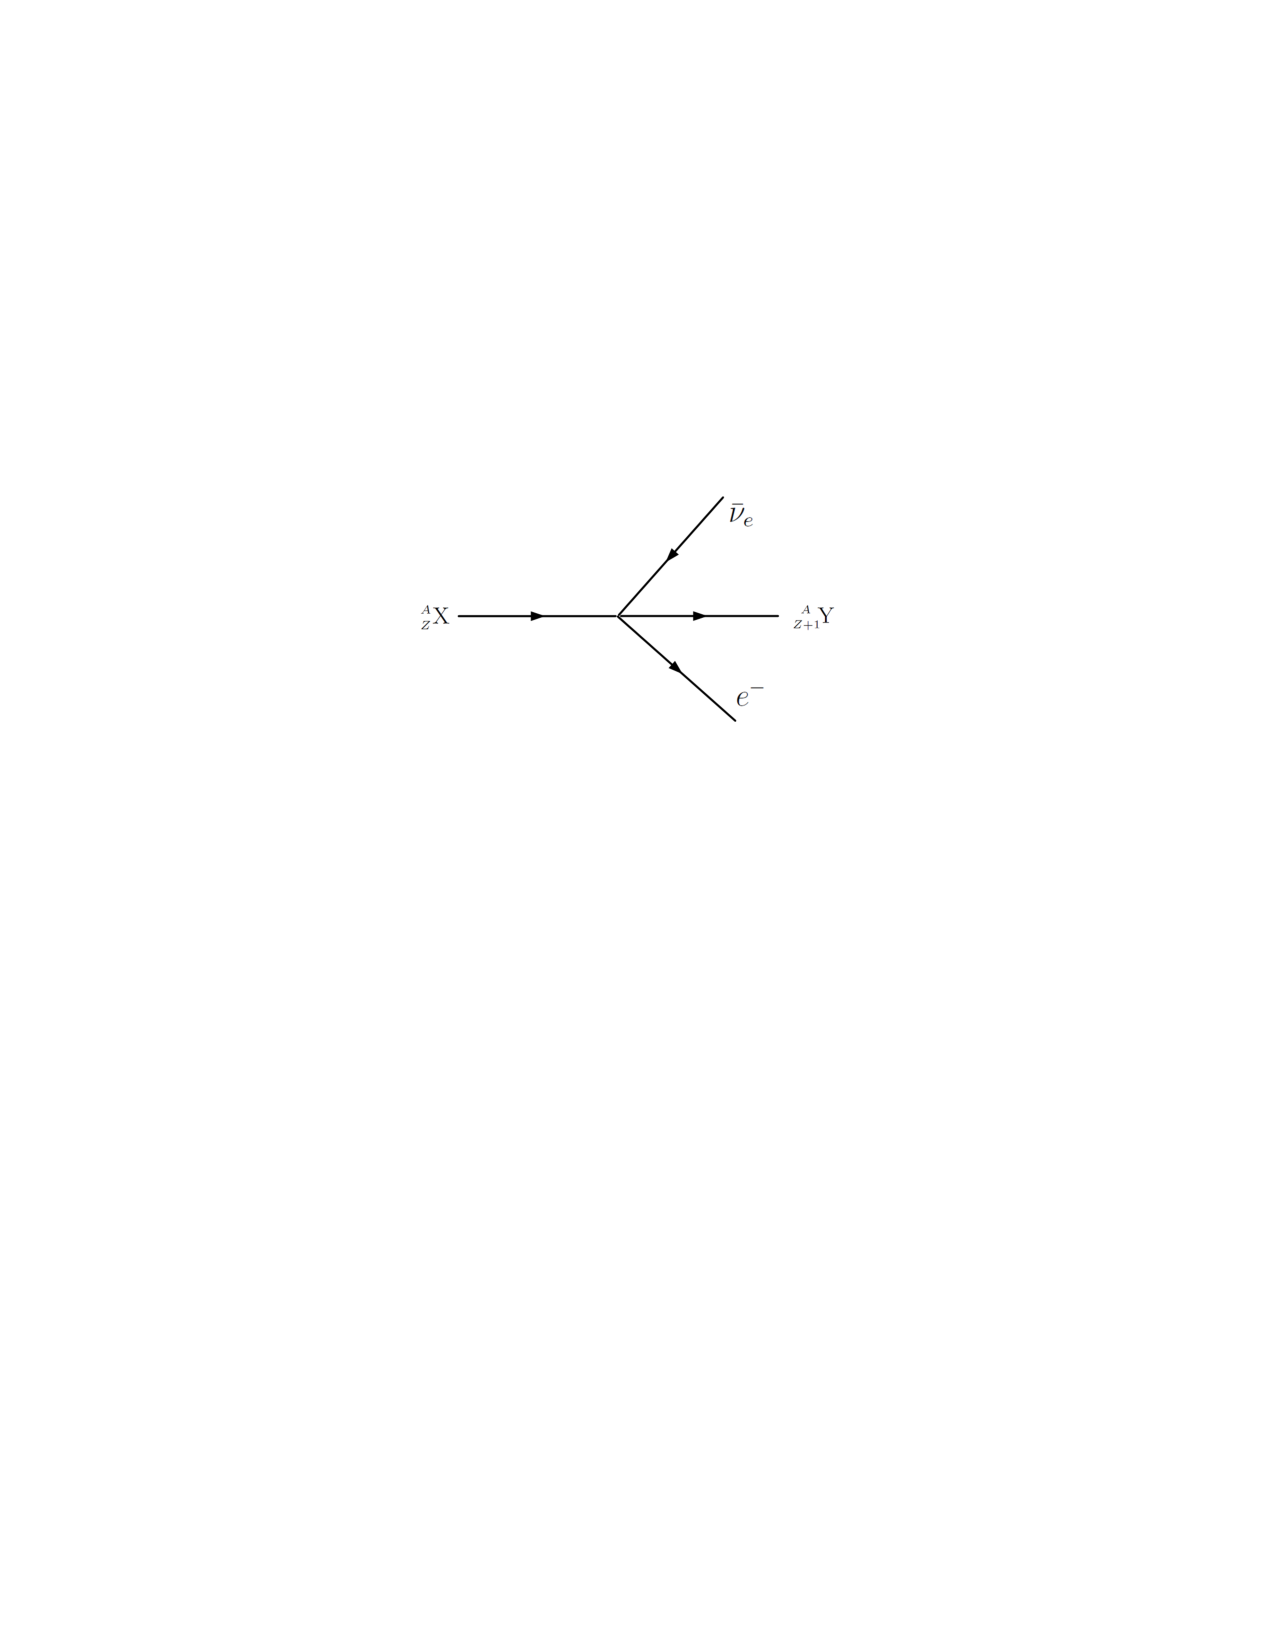
\includegraphics[width=0.7\linewidth]{figures/fermidecay.pdf}
    \caption{Feynman diagram of the $\beta$-decay of a $^{A}_{Z}X$ into a $^{A}_{Z+1}Y$ nucleus in the Fermi approximation.}
    \label{fig:fermibeta}
\end{figure}

This theory paved the way for the first experimental direct detection of neutrinos by Cowan and Reines in 1956 \cite{Cowan:1992xc}, which exploited the inverse $\beta$-decay process:
\begin{equation}
    \bar{\nu}_{e} + p \rightarrow e^{+} + n.
\end{equation}
The key detection technique, still used in modern reactor experiments, employed the detection of the $e^{+}e^{-}\rightarrow 2\gamma$ annihilation and the $\gamma$ emitted by the capture of the recoiling neutron shortly afterwards. 

The leptonic current $\bar{\nu}_{e}\Gamma_{L}e$ was later hypothesised to be left-handed in the form of $\gamma_{\mu}(1-\gamma_{5})$ ($V-A$) by Feynman and Gell-Mann \cite{Feynman:1958ty}.
For massless neutrinos this allows to assign a left-handed (right-handed) helicity to neutrinos (anti-neutrinos), which was experimentally verified by Goldhaber \cite{Goldhaber:1958nb}.

\section{Neutrino Oscillations Theory}
In the modern Standard Model of particle physics there are three flavours of (anti)neutrinos ($\nu_{e}$, $\nu_{\mu}$, $\nu_{\tau}$), each one paired to a charged (anti)lepton ($e$, $\mu$, $\tau$ respectively). 
However, if neutrinos have masses, it is possible to have three (or more) neutrino mass eigenstates ($\nu_{1}$, $\nu_{2}$, $\nu_{3}$, ...) analogues of the charged-lepton mass eigenstates. 
In this case, a neutrino produced as a flavour eigenstate would \emph{oscillate} through its path and change to another flavor eigenstate. This happens because the flavour eigenstate is a mixture of the three (or more) mass eigenstates, which travel with different wavelengths and create interference patterns. 

The oscillation probabilities can be derived in the case of two neutrino generations, which we report here for didactic reasons largely following the approach in \cite{deGouvea:2004gd}. The flavour eigenstates $\nu_{\alpha}, \nu_{\beta}$ can be expressed as a superposition of the two mass eigenstates $\nu_1$ and $\nu_2$ using the nominal rotation matrix $U$:
\begin{equation}
U = \begin{bmatrix}
    \cos\theta & -\sin\theta \\
    \cos\theta & \sin\theta
    \end{bmatrix}.
\end{equation}

The flavour neutrino $\nu_{\alpha}$ will then propagate as: 
\begin{equation}
    \ket{\nu_{\alpha}} = \cos\theta\ket{\nu_{1}}+\sin\theta\ket{\nu_{2}}
\end{equation}

The time evolution of this superposition can be written, in the plane-wave assumption, as:
\begin{equation}
    \ket{\nu(\vec{x},t)} = \cos\theta e^{-ip_{1}x}\ket{\nu_{1}}+\sin\theta e^{-ip_{1}x}\ket{\nu_{2}}.
\end{equation}
If the neutrino is ultra-relativistic the exponential argument becomes:
\begin{equation}
\begin{split}
    p_{i}x & = E_{i}t - \vec{p}_{i}\vec{x} \simeq (E_{i}-p_{z,i})L\\
           & = (E_{i}^2-|\vec{p}|^{2})/(E_{i}-p_{z,i})L\\
           & \simeq m_i^{2}/2E_{i}L \simeq m_i^{2}/2E L,
\end{split}
\end{equation}
and the oscillation probability of the neutrino with flavour $\alpha$ can be written as:
\begin{equation}
\begin{split}
    P_{\alpha\alpha} & = |\bra{\nu_{\alpha}}\ket{\nu(L)}|^2\\
                     & = 1 - \sin^2 2\theta \sin^2\left(\frac{\Delta m^{2}L}{4E}\right),\label{eq:prob}
\end{split}
\end{equation}
where $\Delta m^{2} \equiv m^2_2-m^2_1$ is the mass splitting between the two mass states at play. The probability of observing a neutrino of flavour $\beta$ will be then given by:
\begin{equation}
    P_{\alpha\beta} = 1 - P_{\alpha\alpha} = \sin^2 2\theta \sin^2\left(\frac{\Delta m^{2}L}{4E}\right).\label{eq:prob2}
\end{equation}
Eq. \eqref{eq:prob} and \eqref{eq:prob2} show that the amplitude of the oscillation is regulated by the rotation angle $\theta$, while its frequency depends on the mass splitting, at a fixed $L/E$ ratio. Figure \ref{fig:oscillation} shows as an example the $\nu_e$ survival probability as a function of the neutrino energy for $L=180$~km, $\Delta m^2 = 7.0 \times 10^-5$~ev$^2$ and $\sin^2\theta = 0.84$. 

\begin{figure}
    \centering
    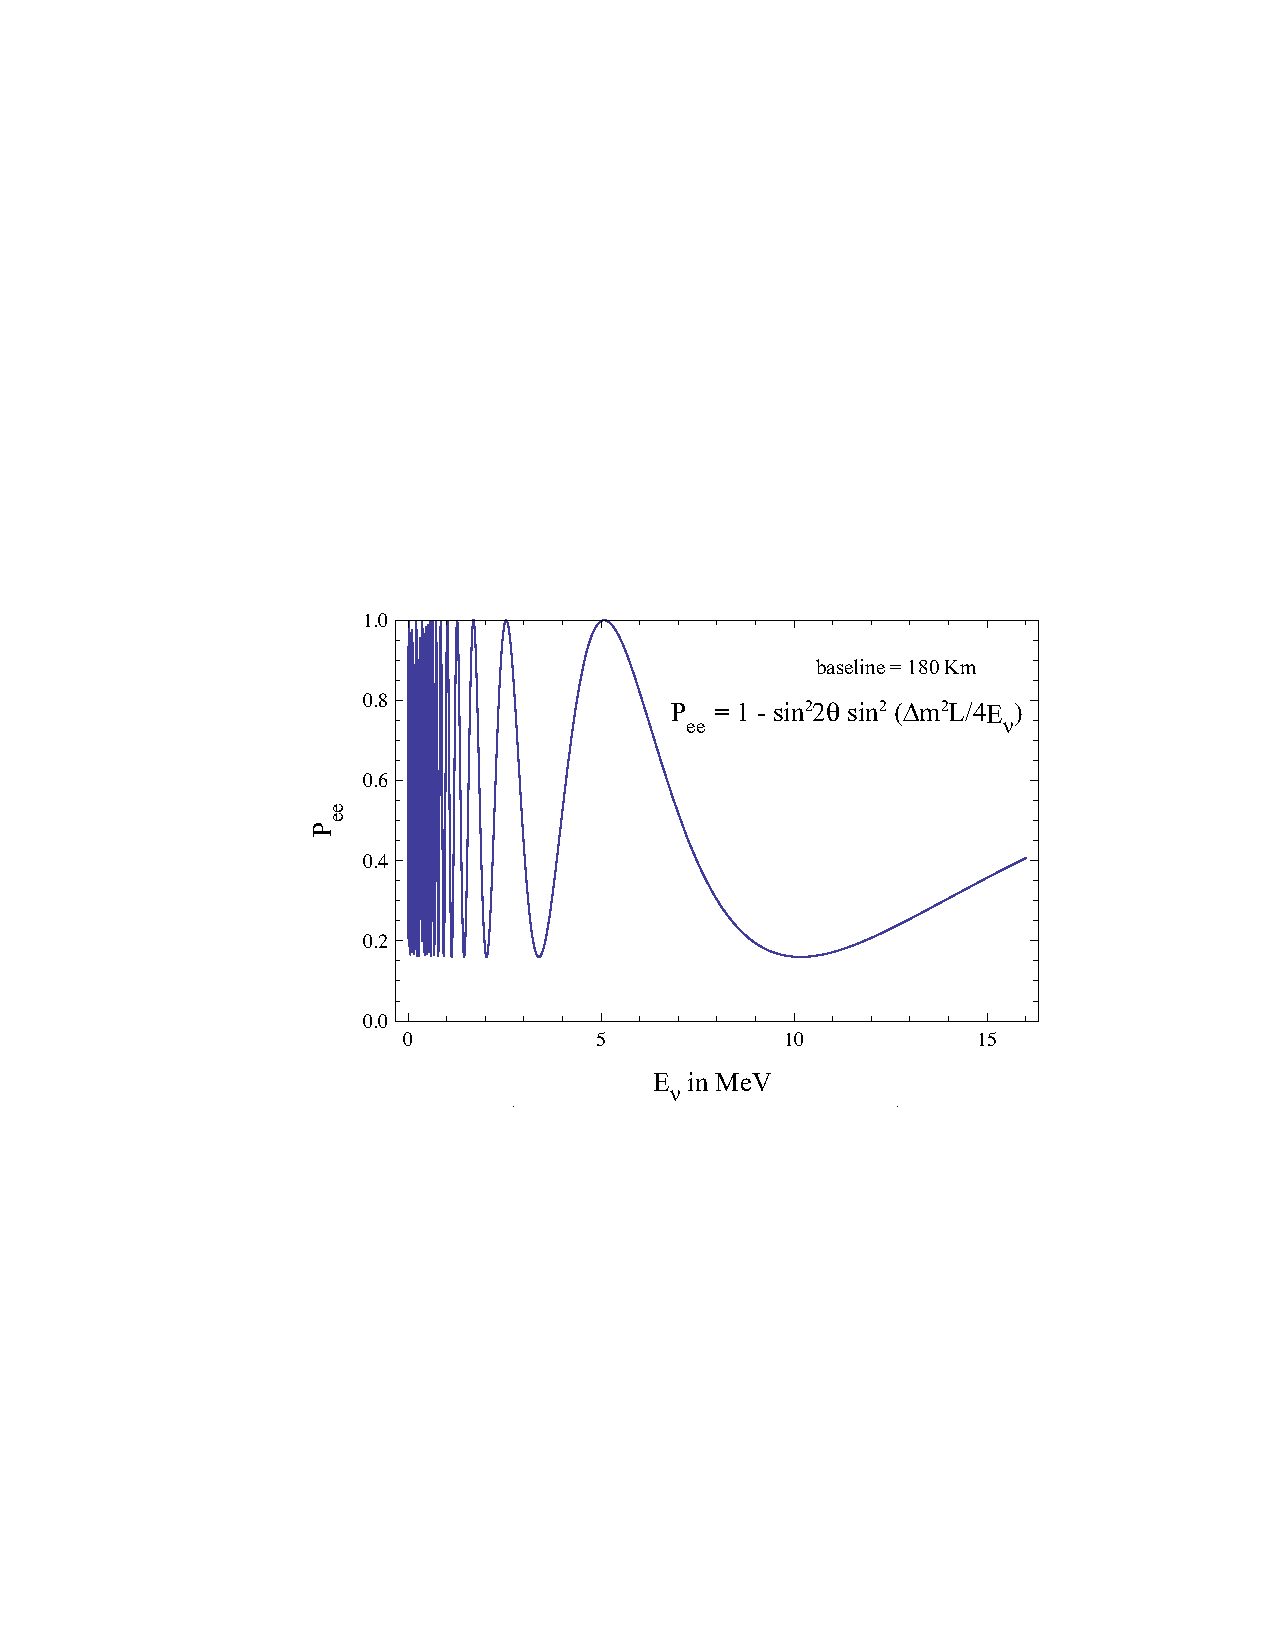
\includegraphics[width=0.7\linewidth]{figures/oscillation.pdf}
    \caption{The $\nu_e$ survival probability $P(\nu_e\rightarrow\nu_e)$ as a function of the neutrino energy for $L=180$~km, $\Delta m^2 = 7.0 \times 10^-5$~ev$^2$ and $\sin^2\theta = 0.84$.}
    \label{fig:oscillation}
\end{figure}

Neutrino oscillations experiments can be divided into two main categories: \emph{disappearance experiments}, which measure the deficit of neutrinos of a certain flavour (measuring $P_{\alpha\alpha}$), and \emph{appearance experiments}, which look for an excess of neutrinos of a certain flavour (measuring $P_{\alpha\beta}$).

The $U$ matrix can be easily extended in the case of the three generations of neutrinos $\nu_{e}$, $\nu_{\mu}$, and $\nu_{\tau}$. In this case, the flavour eigenstates mixing is obtained from:
\begin{equation}
\begin{bmatrix}
\nu_{e}\\
\nu_{\mu}\\
\nu_{\tau}
\end{bmatrix}=
\begin{bmatrix} U_{e 1} & U_{e 2} & U_{e 3} \\ U_{\mu 1} & U_{\mu 2} & U_{\mu 3} \\ U_{\tau 1} & U_{\tau 2} & U_{\tau 3} 
\end{bmatrix} 
\begin{bmatrix} \nu_1 \\ \nu_2 \\ \nu_3 \end{bmatrix},
\end{equation}
where the rotation is given by the so-called Pontecorvo–Maki–Nakagawa–Sakata (PMNS) matrix. It is also possible to parametrise the $U$ matrix in the following useful way:
\begin{align} 
  U_{\mathrm{PMNS}} = \begin{bmatrix} 1 & 0 & 0 \\ 0 & c_{23} & s_{23} \\ 0 & -s_{23} & c_{23} \end{bmatrix}
 \begin{bmatrix} c_{13} & 0 & s_{13}e^{-i\delta_{CP}} \\ 0 & 1 & 0 \\ -s_{13}e^{i\delta_{CP}} & 0 & c_{13} \end{bmatrix}
 \begin{bmatrix} c_{12} & s_{12} & 0 \\ -s_{12} & c_{12} & 0 \\ 0 & 0 & 1 \end{bmatrix},\label{eq:pmns}
\end{align}
where  $s_{ij}$ ($c_{ij}$) is an abbreviation for $\sin\theta_{ij}$ ($\cos\theta_{ij}$) and $\delta^{CP}$ is the CP-violating phase. The mixing angles $\theta_{12}$, $\theta_{13}$, and $\theta_{23}$ are defined by:
\begin{equation}
    \tan^2\theta_{12}\equiv\frac{|U_{e2}|^2}{|U_{e1}|^2},\quad
    \tan^2\theta_{23}\equiv\frac{|U_{\mu3}|^2}{|U_{\tau3}|^2},\quad
    \sin\theta_{13}\equiv U_{e3}e^{i\delta^{CP}}.
\end{equation}

With three neutrino flavours the squared mass-splitting terms are $\Delta m_{12}^2$ and $\Delta m_{13}^2$. This cause a degeneracy in the ordering of three masses: it is possible to have $m_3 > m_2 > m_1$ (\emph{normal hierarchy}) or $m_3 > m_1 > m_2$ (\emph{inverted hierarchy}). Customarily, $\Delta m_{12}^2$ and $\Delta m_{13}^2$ are also called $(\Delta m^2)_{\mathrm{sol}}$ and $(\Delta m^2)_{\mathrm{atm}}$, respectively, since they are usually measured with "solar" and "atmospheric" neutrinos. The situation is illustrated in Figure \ref{fig:masshierarchy}, adapted from \cite{Cahn:2013taa}.

\begin{figure}
    \centering
    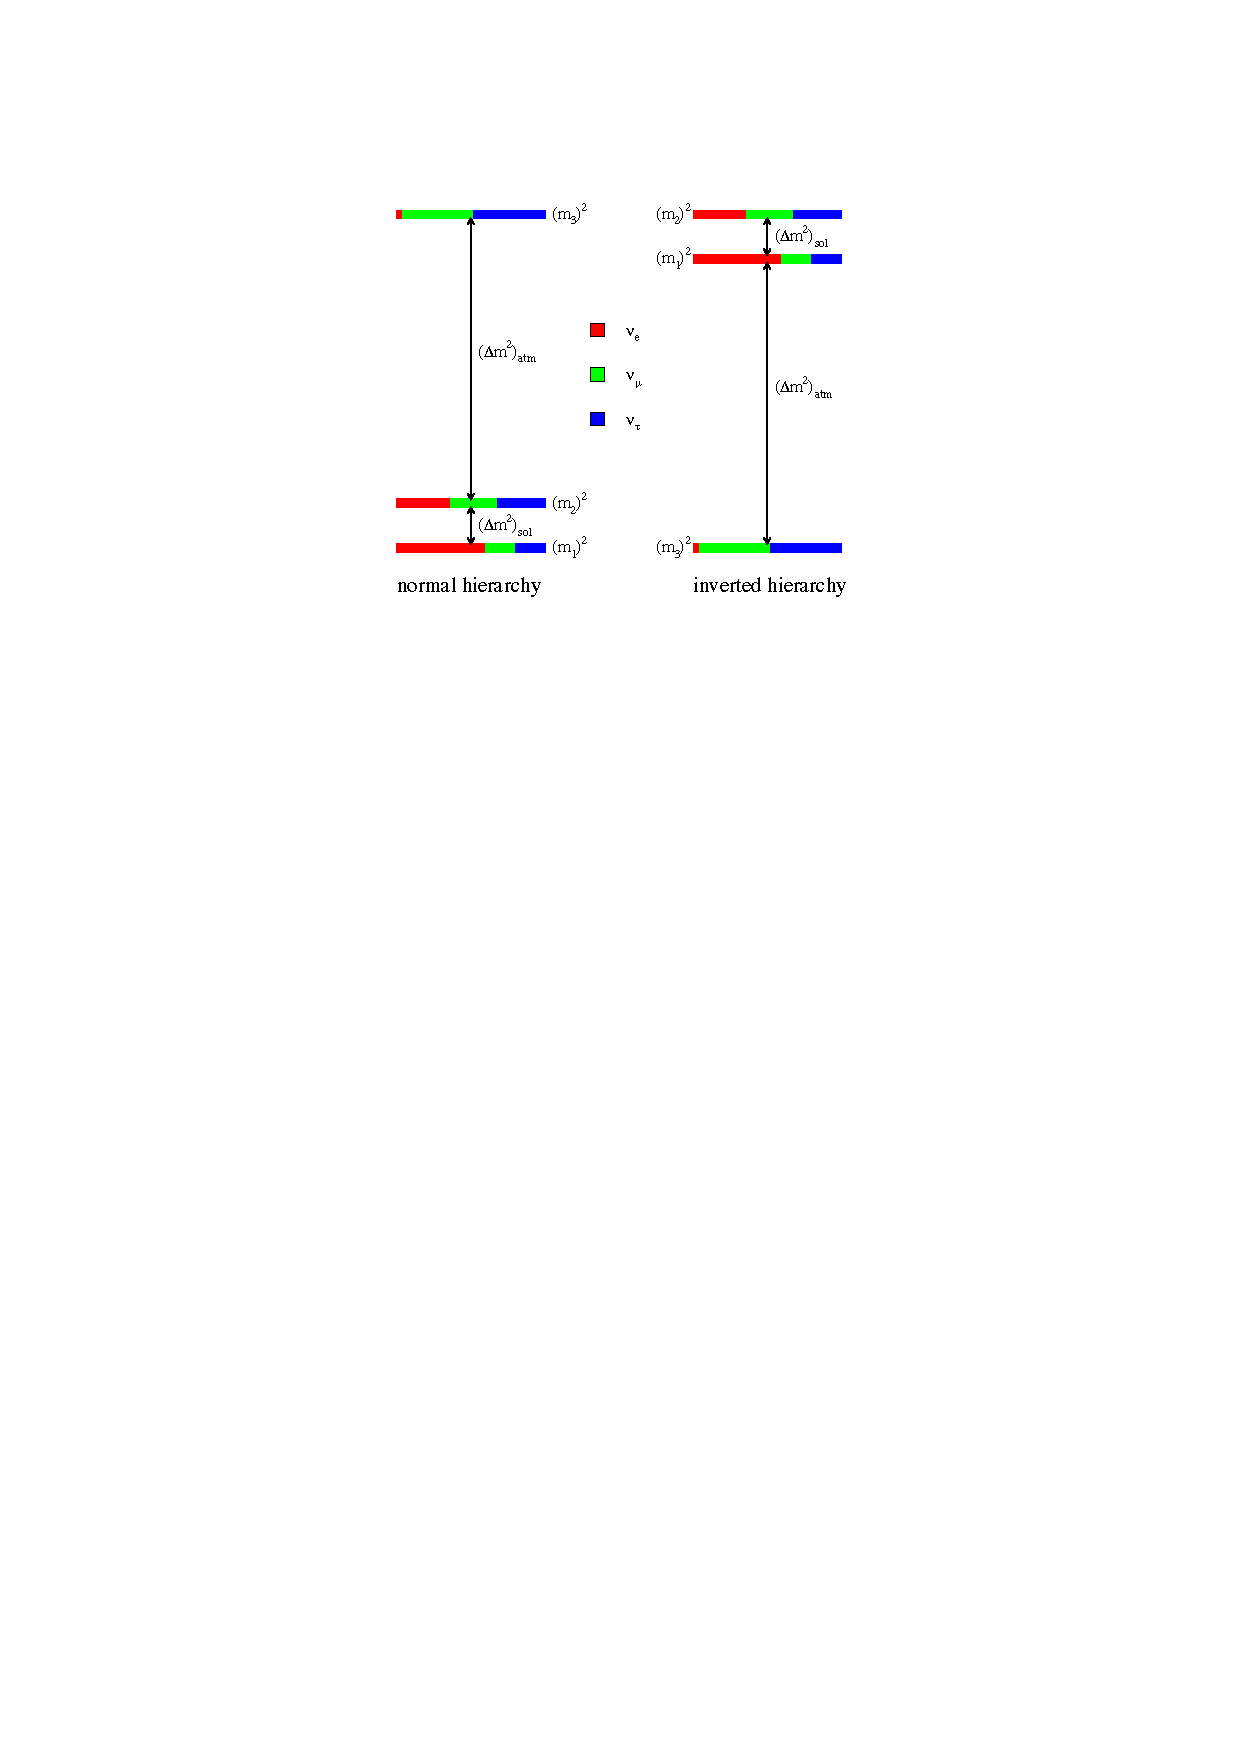
\includegraphics[width=0.75\linewidth]{figures/masshierarchy.pdf}
    \caption{Diagram of the normal and inverted hierarchies. The colours correspond to the fraction of each distinct flavor contained in the mass eigenstate.}
    \label{fig:masshierarchy}
\end{figure}

The mass splittings also determine the $L/E$ ratio at which the oscillation probability is maximised. In the assumption of two-neutrino oscillation, the oscillation frequency in eq. \eqref{eq:prob} becomes:
\begin{equation}
     \frac{\Delta m^{2}L}{4E} = 1.267\left(\frac{L}{\mathrm{km}}\right)\left(\frac{\Delta m^2}{\mathrm{eV}^2}\right)\left(\frac{\mathrm{GeV}}{E}\right),
\end{equation} 
which gives for $\theta_{12}$, $\theta_{13}$, and $\theta_{23}$ a maximum oscillation probability at $\approx 10^4$~km/GeV, $\approx 10^2$~km/GeV, and $\approx 10^2$~km/GeV, respectively. For this reason, $\theta_{12}$, $\theta_{13}$, and $\theta_{23}$ are also known as the \emph{solar}, \emph{reactor}, and \emph{atmospheric} mixing angles. In the parametrisation of the $U_{\mathrm{PMNS}}$ matrix of eq. \eqref{eq:pmns}, the product of the matrices can then be written as:
\begin{equation}
    U_{\mathrm{PMNS}} = U_{\mathrm{atm}} \cdot U_{\mathrm{reactor}} \cdot U_{\mathrm{sol}}.
\end{equation}



\section{Experimental Evidence of Neutrino Oscillation}
After the first direct detection of electron (anti)neutrinos by Cowan and Reines at the Savannah nuclear reactor \cite{Cowan:1992xc}, efforts were made in order to observe the other two neutrino flavours.
In 1962, Lederman and others \cite{PhysRevLett.9.36} first saw evidence of muon neutrinos interacting in the target and producing muons, while the DONUT collaboration finally observed the $\nu_{\tau}$ in 2001 \cite{Kodama:2000mp}.

The number of \emph{light} neutrino species (meaning $m_{\nu} < m_{Z}/2$) weakly interacting was also determined by precision measurements of the $Z$ boson width at LEP and SLD \cite{ALEPH:2005ab} as:
\begin{equation}
   N_{\nu} = \frac{\Gamma_{\mathrm{inv}}}{\Gamma_l}
   \left(\frac{\Gamma_{l}}{\Gamma_{\nu}}\right)_{\mathrm{SM}}=2.984\pm0.008,
\end{equation}
where $\Gamma_{l}$ is the leptonic decay width and $\Gamma_{\mathrm{inv}}$ is the invisible decay width, assumed to be caused by $Z\rightarrow\nu\bar{\nu}$ decays. The lepton universality requires each neutrino flavour to contribute equally. This measurement does not forbid the existence of \emph{heavy} ($m_{\nu} < m_{Z}/2$) or \emph{sterile} (non weakly-interacting) neutrinos.

However, the amount of neutrino interactions observed by several experiments was in disagreement with the one predicted by the theory of three massless neutrinos. In particular, two types of anomalies were identified, one involving the detection of solar neutrinos and one involving the neutrinos produced by cosmic rays in the atmosphere.

\paragraph{Solar neutrino anomaly}
The experiment by Ray Davis and others at Homestake was the first to directly detect the neutrinos produced in the sun \cite{Davis:1968cp} by the $^7$Be and $^8$B decays (Figure \ref{fig:solar}). 

\begin{figure}[htbp]
    \centering
    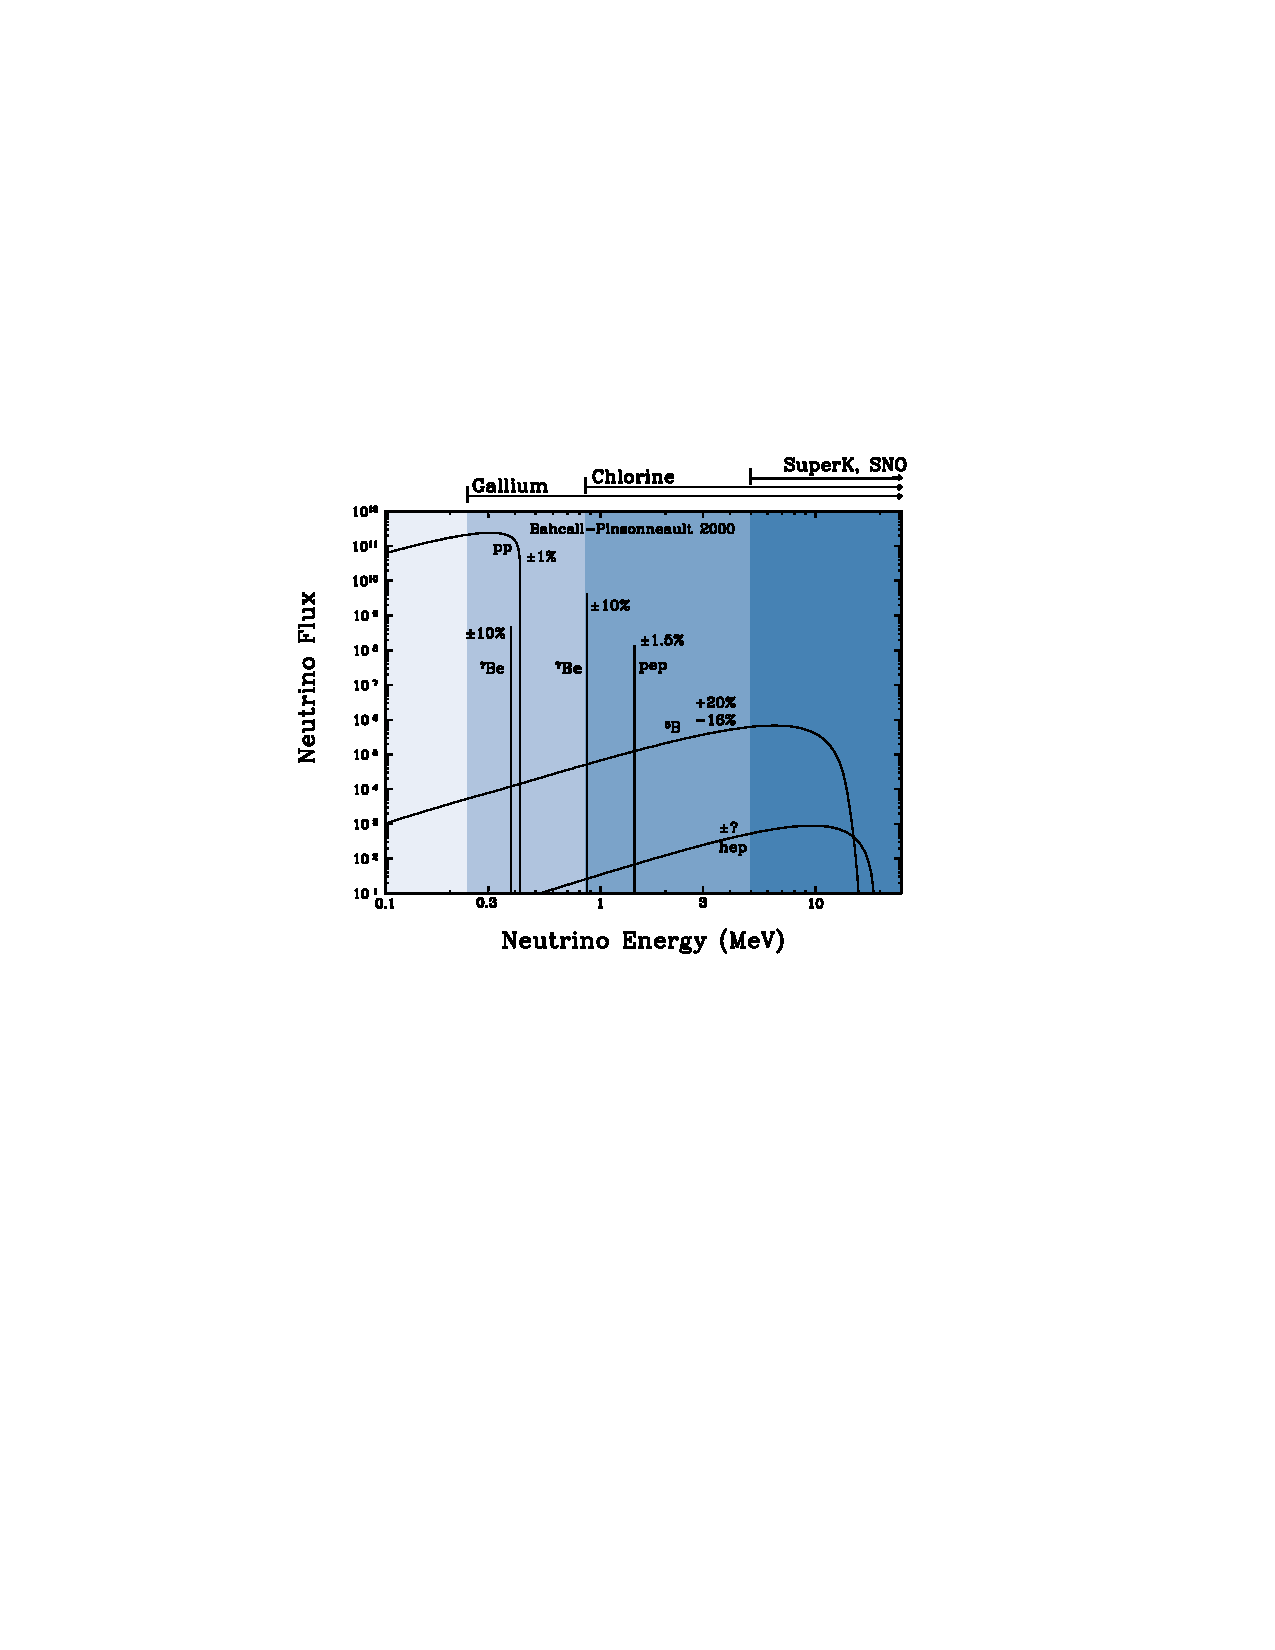
\includegraphics[width=0.75\linewidth]{figures/solar.pdf}
    \caption{The solar neutrino energy spectrum predicted by the solar standard model. Adapted from \cite{Bahcall:2000nu}.}
    \label{fig:solar}
\end{figure}

However, the number of solar neutrino interactions was lower than expected and this deficit was later confirmed by several other experiments, including the Kamioka Observatory in Japan \cite{Hirata:1989zj}, the SAGE experiment in Russia \cite{Abdurashitov:1994bc}, and the GALLEX experiment in Italy \cite{Hampel:1998xg}. The SNO (Sudbury Neutrino Observatory) experiment finally proved in 2001 that the cause of the deficit was the oscillation of the solar neutrinos into a different flavour eigenstate \cite{Ahmad:2002jz}, by measuring both the solar $\nu_{e}$ flux and the total solar neutrino flux, as shown in Figure \ref{fig:sno}. 

\begin{figure}[htbp]
    \centering
    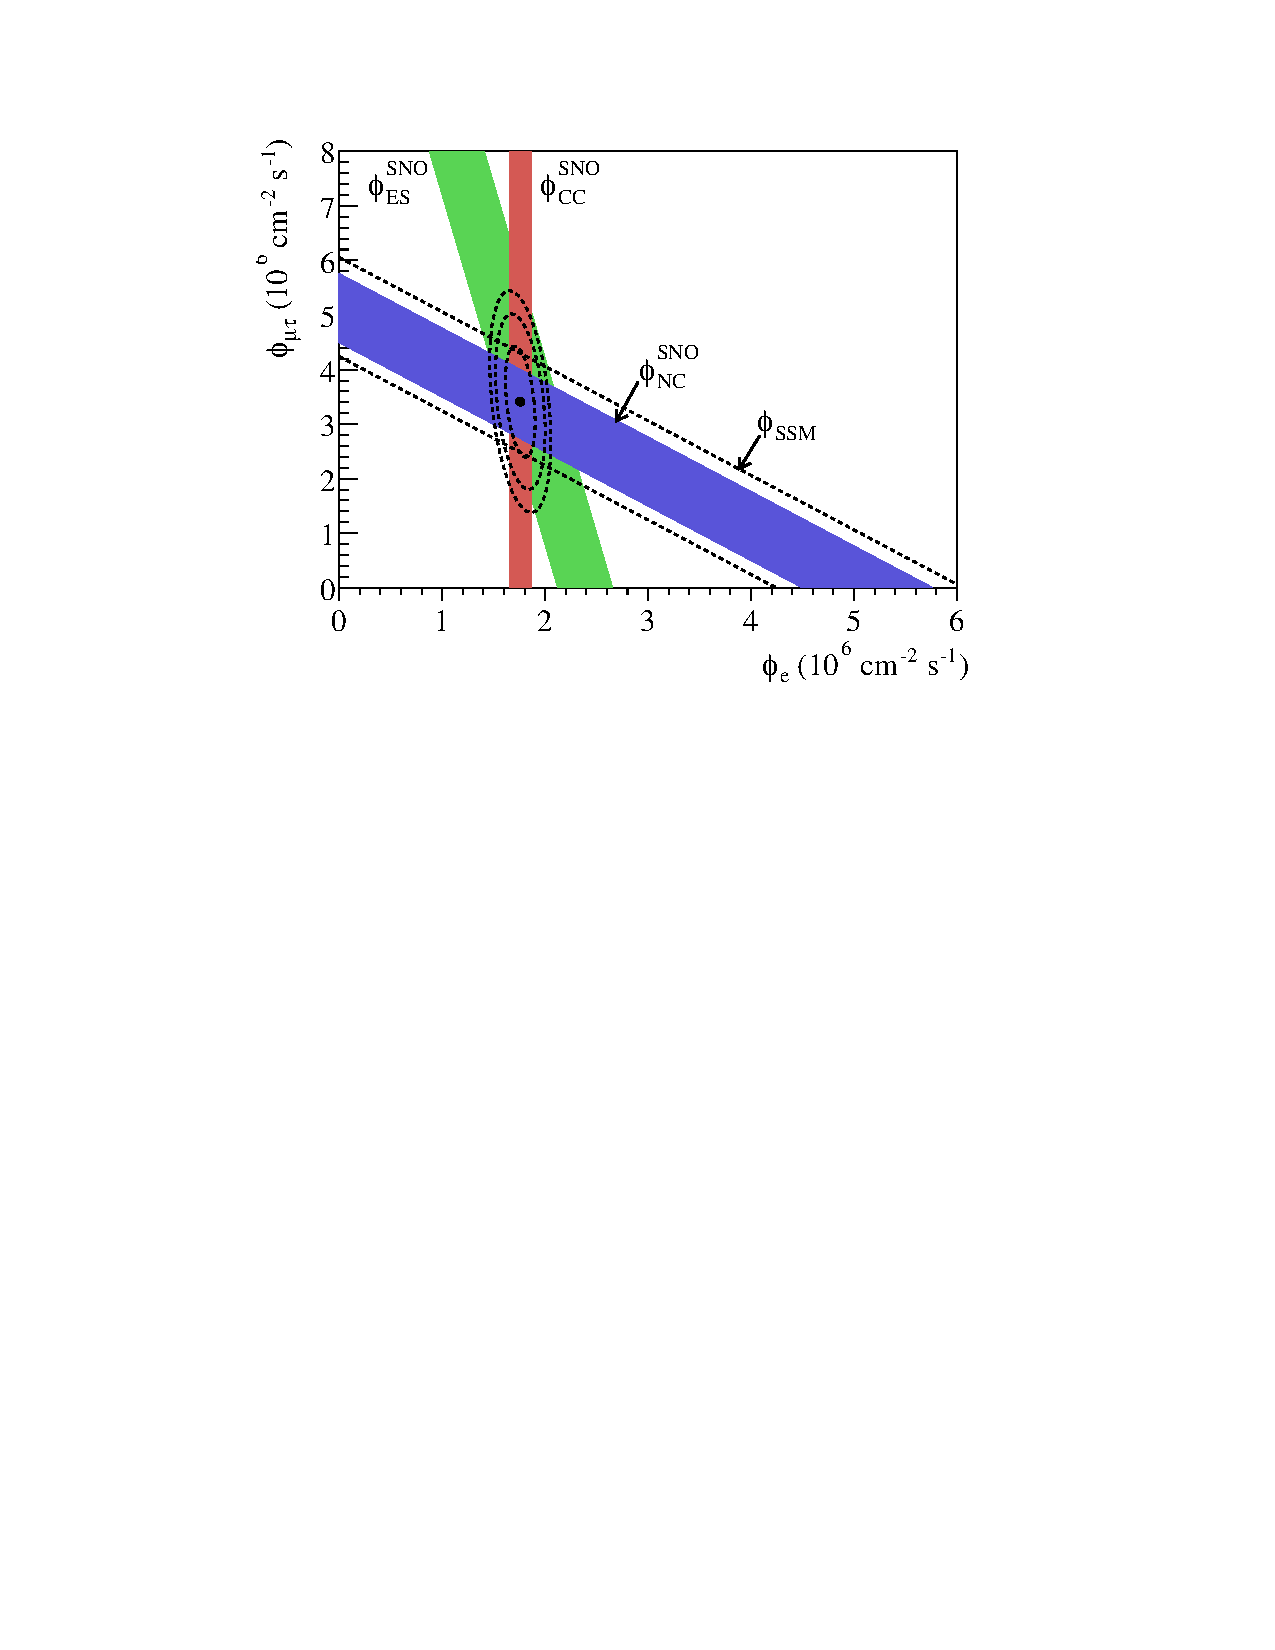
\includegraphics[width=0.7\linewidth]{figures/sno_plot.pdf}
    \caption{SNO measurement of the neutral-current ($\phi_{\mathrm{NC}}$), charged-current ($\phi_{\mathrm{CC}}$), and elastic scattering ($\phi_{\mathrm{ES}}$) fluxes. The CC measurement is sensitive to the $\nu_e$ flavour only, while the NC and ES fluxes depend both on $\nu_e$ and $\nu_{\mu}$/$\nu_{\tau}$ interactions. The neutrino flux predicted by the SSM (Standard Solar Model) is given by $\phi_{\mathrm{SSM}}$.}
    \label{fig:sno}
\end{figure}

The propagation of neutrinos in the matter is determined by the Mikheyev-Smirnov-Wolfenstein (MSW) effect \cite{Wolfenstein:1977ue}: in presence of a high density of electrons, electron neutrinos experience a charged current coherent forward scattering. This cause the electron neutrinos to have a different effective mass when they propagate in a high-density medium, modifying the oscillation pattern. 

The MSW effect is particularly important to explain the solar neutrino flux (Figure \ref{fig:solar}). Assuming a very high electron density in the sun core and an exponentially decreasing abundance (which are both good approximations in the standard solar model), the probability to observe an electron neutrino when it reaches the Earth is $P_{ee} \approx \sin^2\theta$ for neutrinos above 2~MeV (where the matter effect dominates).


\paragraph{Atmospheric neutrino anomaly}
Cosmic muons decaying in the atmosphere produce a broad flux of muon (antineutrinos). The first underground water Cherenkov detectors, the IMB experiment and the Kamioka observatory, observed a discrepancy in the double ratio of muon to electron neutrinos, measured to expected. The evidence that this discrepancy was caused by the disappearance of atmospheric neutrinos was provided by the Super-Kamiokande experiment in 1998 \cite{Fukuda:1998mi}.

Figure \ref{fig:superk} shows the zenith angle distributions of events detected by the Super-Kamiokande experiment: the data points are in disagreement with the no-oscillation model and they can be interpreted as $\nu_{\mu} \leftrightarrow \nu_{\tau}$ oscillation.

In honour of these discoveries, the Nobel Prize in Physics 2015 was awarded to Takaaki Kajita (Super-Kamiokande) and Arthur B. McDonald (SNO). 

\begin{figure}[htbp]
    \centering
    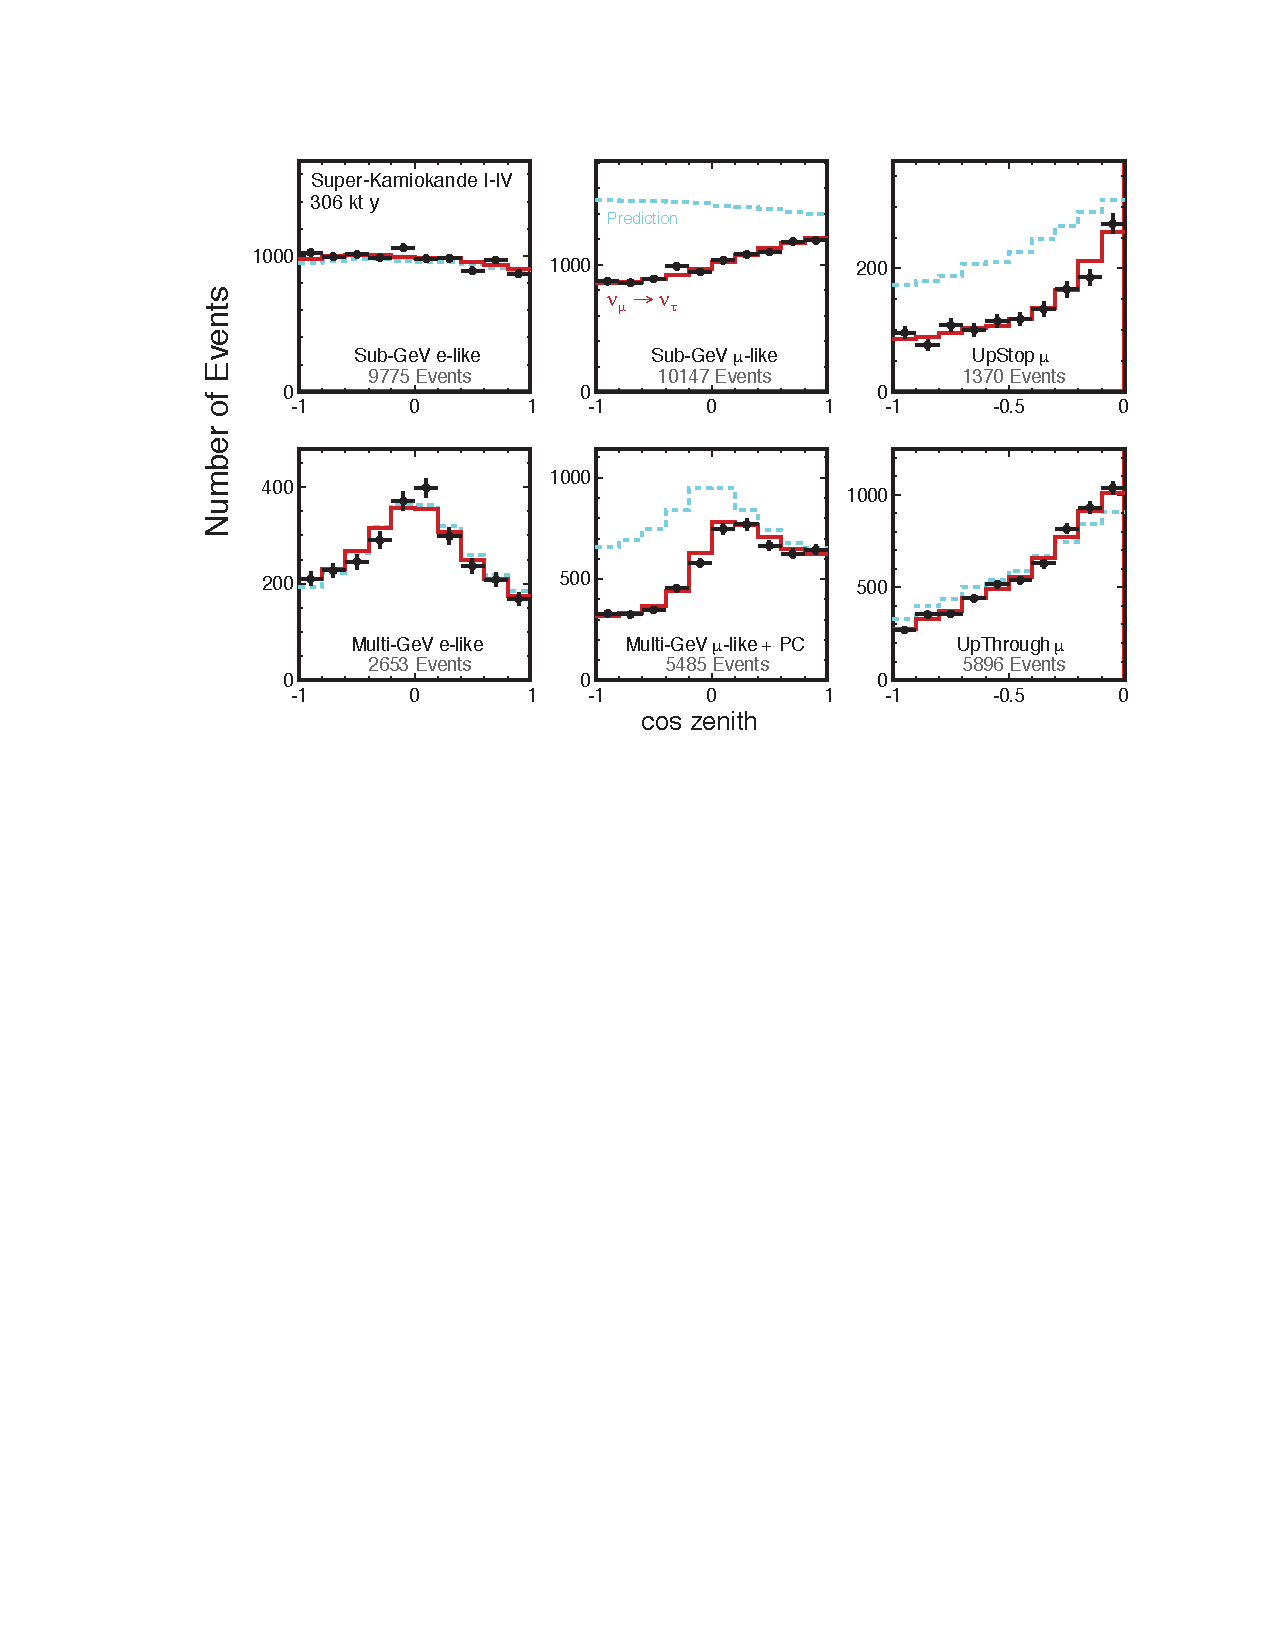
\includegraphics[width=0.9\linewidth]{figures/superk.pdf}
    \caption{Zenith angle distributions of $\mu$-like and e-like events in the sub-GeV and multi-GeV data sets, as collected by the Super-Kamiokande experiment. The dashed blue line corresponds to the no-oscillation model. The red solid line represent the best fit to $\nu_{\mu} \leftrightarrow \nu_{\tau}$ oscillation (from \cite{PhysRevD.98.030001}).}
    \label{fig:superk}
\end{figure}

\vspace{1em}

The KamLAND experiment finally spectacularly proved the oscillation pattern and the MSW model by measuring the reactor electron antineutrinos survival probability as a function of $L/E$, shown in Figure \ref{fig:kamland}. 

\begin{figure}[htbp]
    \centering
    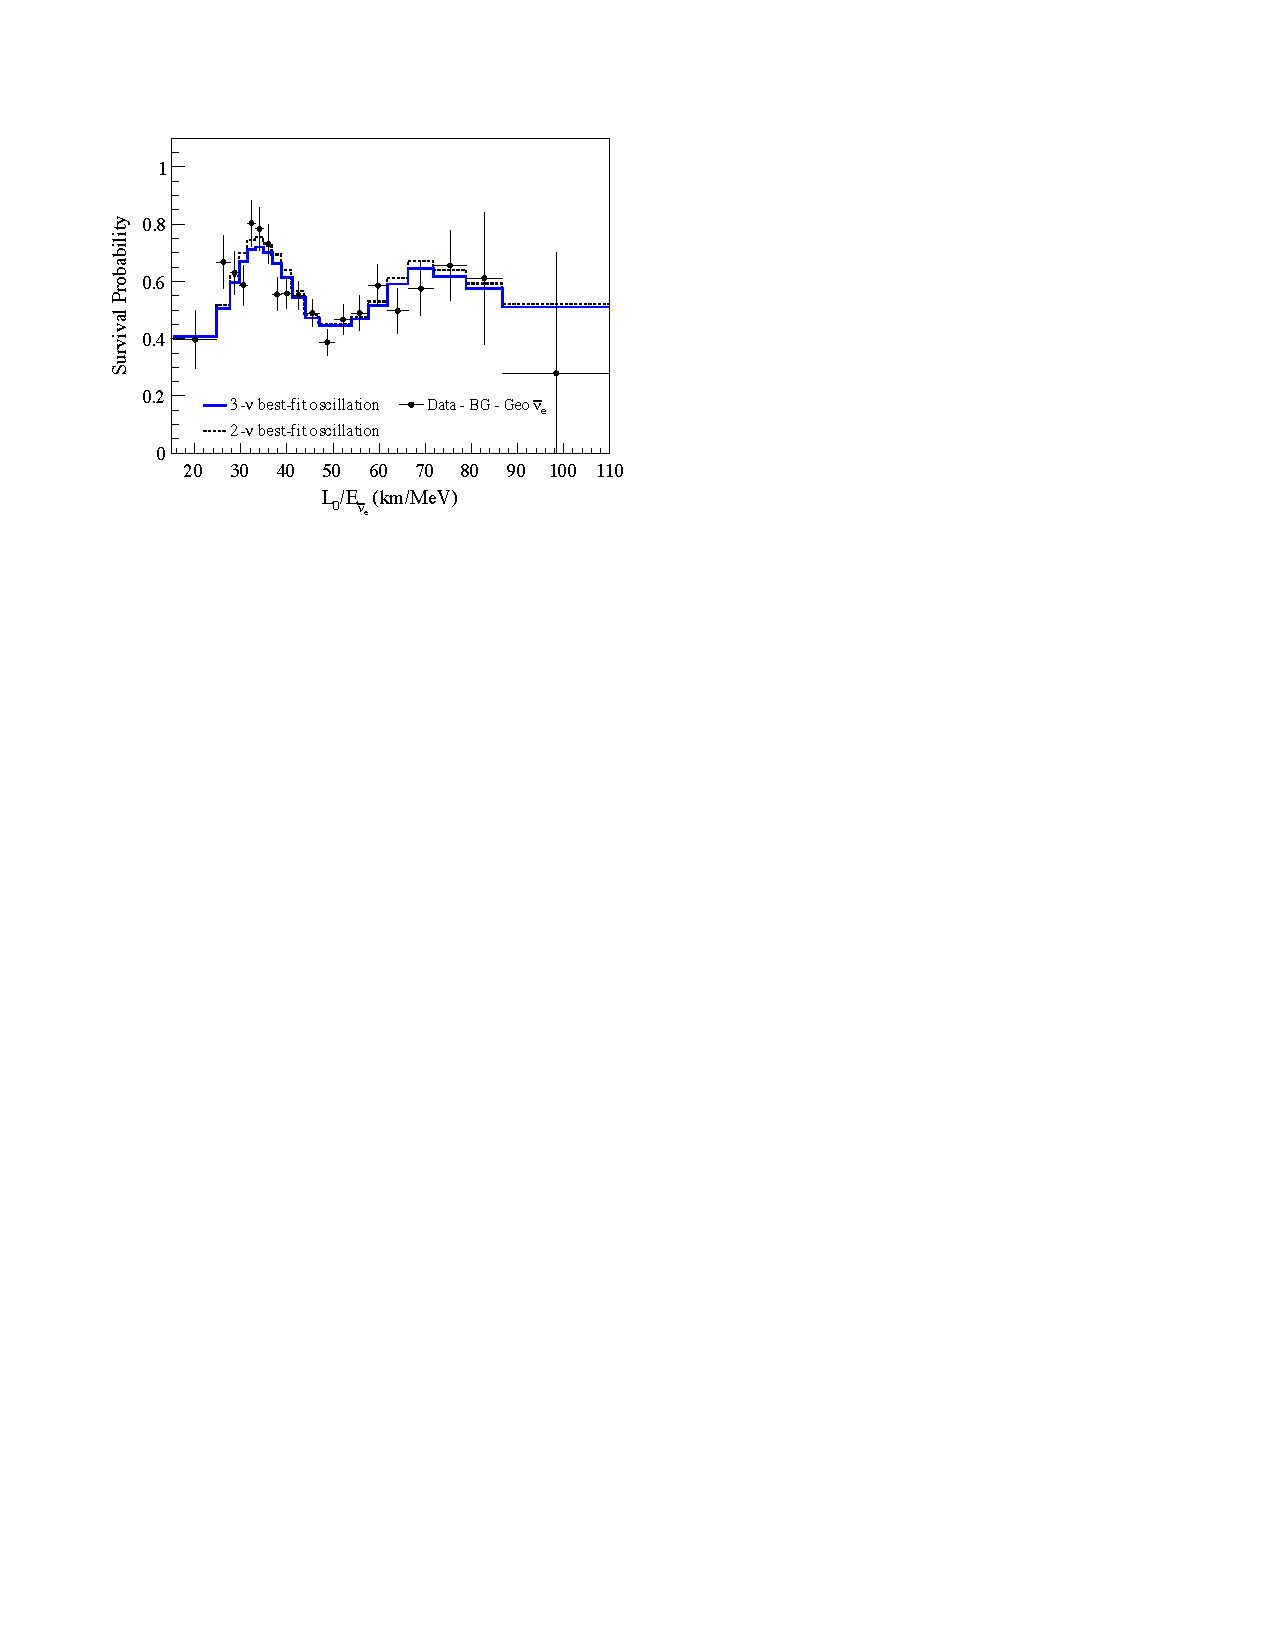
\includegraphics[width=0.75\linewidth]{figures/kamland.pdf}
    \caption{Ratio of the observed $\bar{\nu}_{e}$ spectrum to the expectation for no-oscillation versus $L_{0}/E$ for the KamLAND data. $L_{0} = 180$~km is the flux-weighted average reactor baseline (from \cite{Gando:2010aa}).}
    \label{fig:kamland}
\end{figure}

Less than 20 years after the definitive confirmation of neutrino oscillations, the mixing angles and the mass splittings are all known with a relative uncertainty smaller than 5\%. The least-known parameter in the PMNS matrix is the $\delta_{CP}$ phase, which, if different from $0^{\circ}$ (or from $180^{\circ}$), would imply CP-violation in the leptonic sector. This parameter can be measured only with appearance experiments, where it is possible to verify if
$P(\nu_{\alpha}\rightarrow\nu_{\beta}) \neq P(\bar{\nu}_{\alpha}\rightarrow\bar{\nu}_{\beta})$. Recent results from the T2K and NOVA experiments give a best fit of $\delta_{CP}/^{\circ}=215^{+40}_{-28}$  ($\delta_{CP}/^{\circ}=284^{+27}_{-29}$) at $1\sigma$ in the normal hierarchy (inverted hierarchy) model \cite{Esteban:2018azc}. A definitive measurement of the CP-violating phase would have far-reaching consequences in particle physics and cosmology, since it could explain the matter-antimatter asymmetry, providing an experimental basis for the leptogenesis model \cite{Fukugita:1986hr}.

A precise estimation of the MSW effect is particularly important for a correct measurement of the CP violation. Since the matter contains electrons and not positrons, the electron neutrinos will experience a MSW effect opposite to the one experienced by antineutrinos. This difference will, in turn, modify the appearance probabilities, leading to $P(\nu_{e}\rightarrow\nu_{\mu}) \neq P(\bar{\nu}_{e}\rightarrow\bar{\nu}_{\mu})$. This effect must the be disentangled from the CP-violating effect caused by the complex phases in the PMNS matrix.

The MSW effect is also dependent on the sign of the mass splitting $\Delta m_{31}$, which offers a way to resolve the hierarchy problem \cite{Smirnov:2013cqa}. 
In this document, however, we will focus on short-baseline neutrino experiments, where the MSW effect is negligible.

\section{Massive neutrinos in the Standard Model}
The observation of neutrino oscillations poses a challenge for the SM, since it requires a mechanism able to give mass to the neutrinos.
In the standard formulation of the SM, quarks and leptons can be represented by a four-component Dirac spinor field $\psi_{D}$. This field can be decomposed into left-handed and right-handed two-component spinors with the chirality operators $\chi_{R} = (1+\gamma_5)\psi_D$ and $\chi_{L} = (1-\gamma_5)\psi_D$, respectively. The mass term for these spinors can be generated through the Higgs mechanism, which introduces a Dirac mass term in the Lagrangian:
\begin{equation}
    -\mathcal{L}_D = m_D\bar{\psi}_D\psi_D = m_D(\bar{\nu}_L\nu_R + \bar{\nu}_R\nu_L).
\end{equation}
This term breaks chirality symmetry and makes helicity non-Lorentz-invariant and can be applied also to neutrinos in an extension to the Standard Model. In this case, the neutrino would be a four-component massive Dirac spinor, just as any other fermion, with two components non-interacting.
However, the current upper limit on the sum of the neutrino masses is $\sum m_{\nu} < 0.12$~eV using cosmological constraints \cite{Aghanim:2018eyx} and $\sum m_{\nu} < 2$~eV from $\beta$-decay experiments \cite{Otten:2008zz}. The KATRIN experiment will directly measure the neutrino mass through a precise reconstruction of the tritium $\beta$-decay spectrum, with an expected sensitivity of 0.2~eV \cite{Osipowicz:2001sq}. These results require a Yukawa coupling six orders of magnitude smaller than the electron one, which is not considered natural. 

Most importantly, right-handed (left-handed) neutrinos (antineutrinos) have never been observed. Their existence would be theoretically motivated, since quarks and leptons have right-handed components and they could explain the small neutrino masses, as described in Section \ref{sec:seesaw}. Right-handed neutrinos would interact only gravitationally and for this reason they are usually called \emph{sterile neutrinos}. Even if not weakly-interacting, the eventual sterile neutrino(s) would still mix with the active flavours, affecting the measured oscillation patterns and providing an experimental detection signature.

Another model for the neutrino masses would be the introduction of a Majorana mass term in the Lagrangian:
\begin{equation}
    -\mathcal{L}_M = \frac{1}{2}m_M(\bar{\nu}_L\mathcal{C}\bar{\nu}^{T}_L+\nu_{L}\mathcal{C}\nu^T_L) = \frac{1}{2}m_M(\bar{\nu}_M\nu_M), \label{eq:majorana}
\end{equation}
where the factor $\frac{1}{2}$ accounts for double-counting due to the hermitian conjugate being identical, $\nu_{M} \equiv \nu_L + \nu^c_R$ is the Majorana spinor, and $\mathcal{C}$ is the charge-conjugation operator. Here, the charge-conjugation operator must leave the field unchanged and the particle must then be neutral.

The only fermion that satisfies this requirement is the neutrino. If the neutrino is a Majorana particle, it will be its own antiparticle: in a CC interaction, the left-handed and right-handed components would produce a negative-charged and a positive-charged lepton, respectively.

An experimental evidence of the Majorana nature of the neutrinos would be the observation of the neutrinoless double $\beta$ decay ($0\nu\beta\beta$), where a $\nu_{e}$ is emitted and absorbed in the nucleus, producing two electrons and two protons in the final state. Figure \ref{fig:0vbb} shows the Feynman diagram for a $0\nu\beta\beta$ interaction. 

\begin{figure}[htbp]
    \centering
    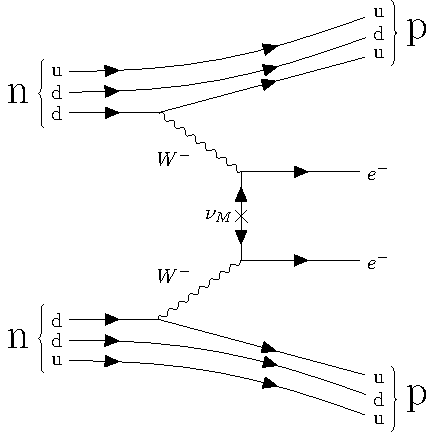
\includegraphics[width=0.55\linewidth]{figures/0vbb.pdf}
    \caption{Feynman diagram for a neutrinoless double beta decay interaction, emitting two electron in the final state and no neutrinos.}
    \label{fig:0vbb}
\end{figure}

This process would also violate the lepton number with $\Delta L = 2$. In this case, the PMNS matrix in eq. \eqref{eq:pmns} acquires two extra Majorana phases in the form:
\begin{equation}
    U_{PMNS}^M = U_{PMNS} \begin{bmatrix}
    e^{i\alpha} & 0 & 0 \\
    0 & e^{i\beta} & 0 \\
    0 & 0 & 1
    \end{bmatrix}.
\end{equation}

Several experiments are actively looking or planning to look for $0\nu\beta\beta$ decays, using $^{130}$Te (CUORE, SNO+), $^{136}$Xe (KamLAND-Zen, EXO, NEXT), or $^{76}$Ge (GERDA). 
The KamLAND-Zen collaboration measured the lower limit for $0\nu\beta\beta$ decay half-life at $T_{\frac{1}{2}} > 1.07\times10^{26}$~years, which corresponds to an effective Majorana mass of 61-165 meV \cite{KamLAND-Zen:2016pfg}.

\subsection{The Seesaw mechanism}\label{sec:seesaw}
A process which could explain the small masses of the neutrinos, compared to the other fermions, is the so-called \emph{seesaw} mechanism, which here we describe using the approach in \cite{Grossman:2003eb}. 
The most general Lagrangian with right-handed neutrinos can be written as:

\begin{align}
    -2\mathcal{L}_{\mathrm{mass}} & = \mathcal{L}^D_L + \mathcal{L}^D_R + \mathcal{L}^M_L + \mathcal{L}^M_R + h.c. \\
    & = m_D \bar{\nu}_R \nu_L + m_D \bar{\nu}^C_L\nu^C_R + m_L\bar{\nu}_L^C\nu_L + m_R \bar{\nu}_R^C\nu_R.
\end{align}
This term can be expressed as a matrix equation 
\begin{equation}
    -2\mathcal{L_\mathrm{mass}} = \begin{bmatrix}
    \bar{\nu}_L^C & \bar{\nu}_R
    \end{bmatrix}\begin{bmatrix}
    m_L & m_D \\
    m_D & m_R
    \end{bmatrix}\begin{bmatrix}
    \nu_L \\ \nu_R^C
    \end{bmatrix},
\end{equation}
where $m_D$ is the Dirac mass term and $m_L$ ($m_R$) is the Majorana mass term for the left-handed (right-handed) component. 

Since the SM forbids the left-handed Majorana term (it is not gauge invariant), it is possible to set $m_L=0$. For large values of $m_R$, the eigenvalues of the mass matrix are:
\begin{align}
    m_1 & = \frac{m_D^2}{m_R} \\
    m_2 & = m_R \left(1+\frac{m_D^2}{m_R^2}\right) \approx m_R
\end{align}. With a value of $m_R$ at the GUT scale, this would \emph{naturally} give a small value for the neutrino masses. 

The existence of heavy Majorana neutrinos is closely related to the \emph{leptogenesis} hypothesis. In this scenario, the heavy Majorana neutrinos present in the early universe would have decayed into leptons (or antileptons) and Higgs bosons. The so-called \emph{sphaleron} processes would then convert the leptons into baryons and the presence of CP violation in this heavy neutrino sector would then explain the matter-antimatter asymmetry in the universe. It is worth mentioning that this model satisfies the Sakharov conditions \cite{Sakharov:1967dj} for baryogenesis, since it presents baryon number violation, CP violation, and out-of-equilibrium interactions \cite{DiBari:2012fz}.


\section{Neutrino interaction modes}\label{sec:modes}
The interaction between the neutrino and the nucleon can have different forms and a good understanding of their phenomenology is of fundamental importance for the success of any neutrino experiment.
Figure \ref{fig:ccqecross} shows the neutrino cross-section for charged-current interactions divided into three main interaction modes: quasi-elastic (QE), resonant (RES), and deep inelastic scattering (DIS). 

\begin{figure}[htbp]
    \centering
    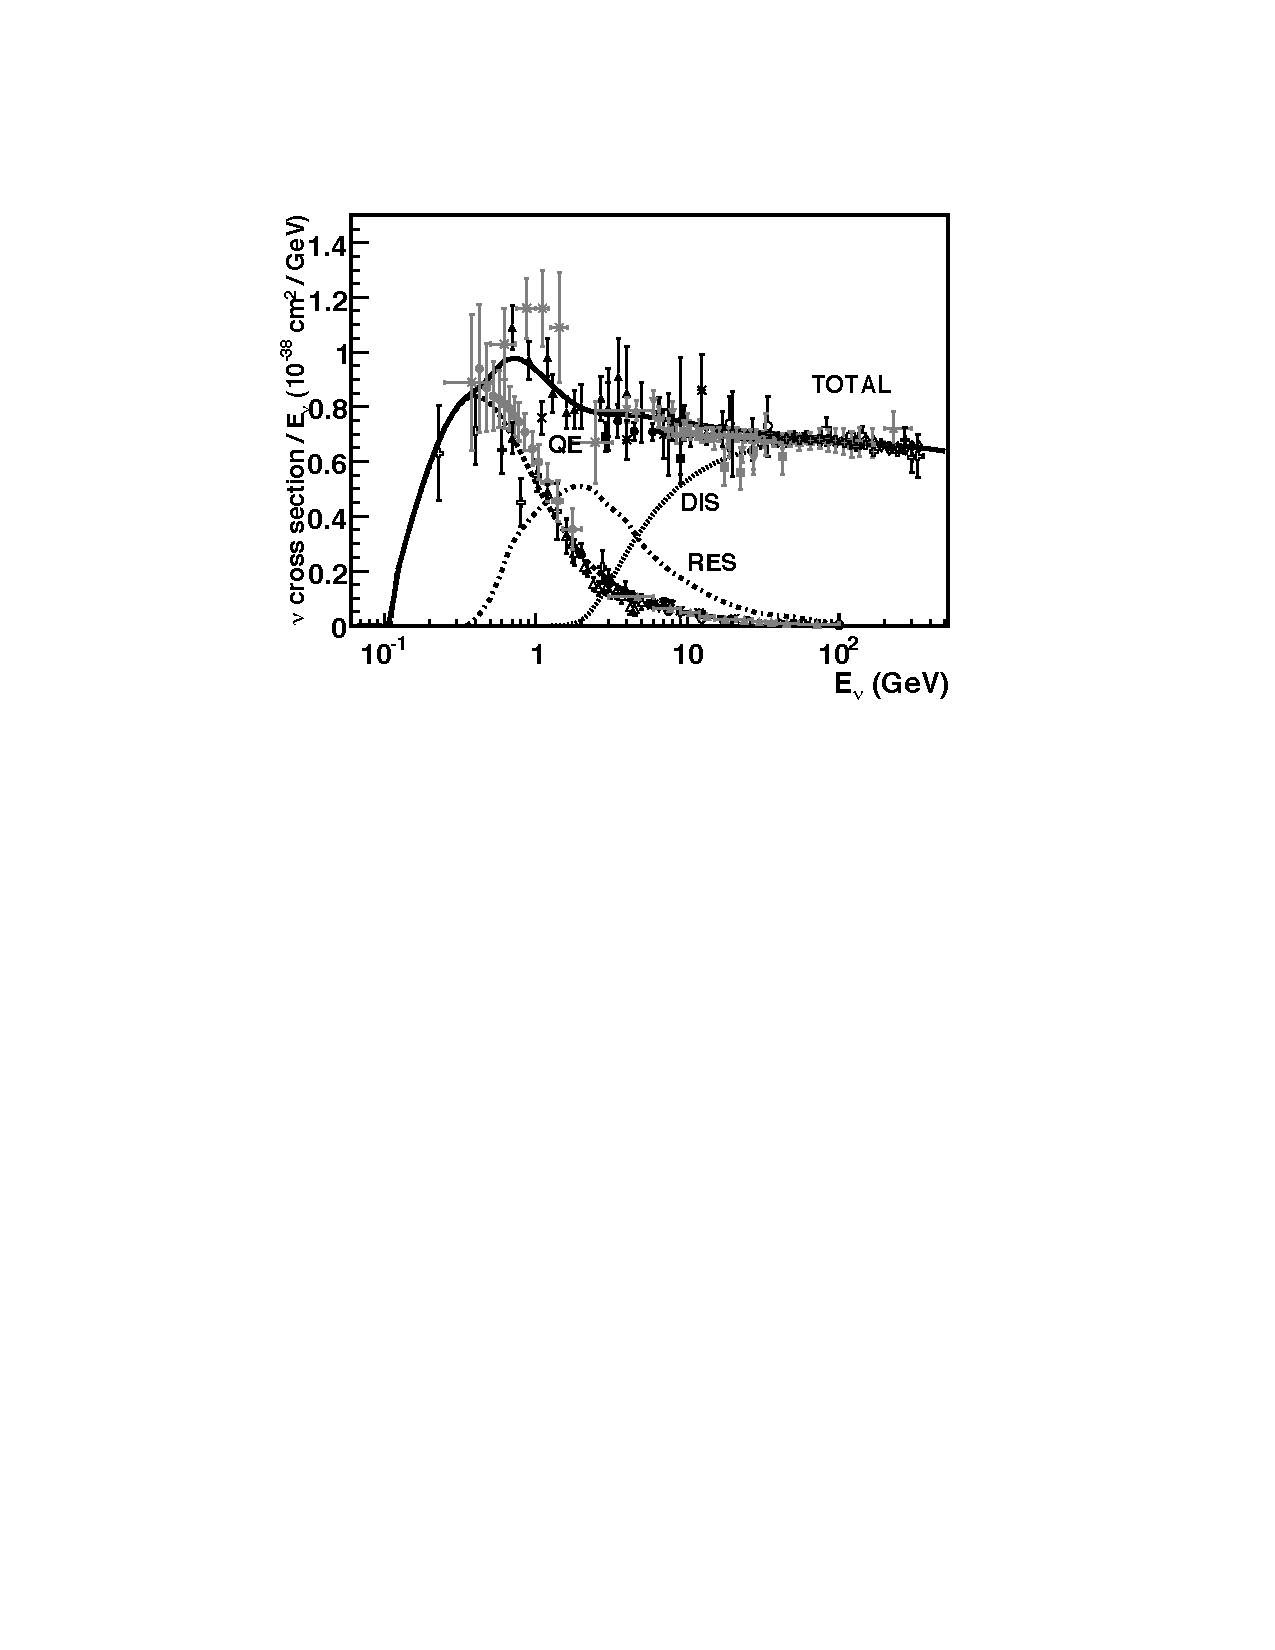
\includegraphics[width=0.7\linewidth]{figures/ccqecross.pdf}
    \caption{Total neutrino per nucleon charged-current cross sections (for an isoscalar target) divided by neutrino energy and plotted as a function of energy (from \cite{Formaggio:2013kya}).}
    \label{fig:ccqecross}
\end{figure}

\begin{description}
\item[Quasi-elastic interaction.] In a charged-current quasi-elastic (CCQE) interaction, the neutrino exchange a $W$ boson with a single nucleon, which is knocked out and leaves a \emph{hole} in the nucleus. Hence its name 1p-1h (one particle, one hole). In this case, the incident neutrino does not have enough energy to break up or excite the nucleus. This is the dominant interaction in the sub-GeV energy range. Figure \ref{fig:ccqe_feyn} shows the Feynman diagram for a CCQE neutrino-nucleus interaction.

The simulation used in this document employs the GENIE neutrino generator, set up to use the Llewellyn-Smith parametrisation for the CCQE interactions \cite{LlewellynSmith:1971uhs} and the Relativistic Fermi Gas model for the nucleus \cite{Smith:1972xh}.
In this model, the interaction is calculated with the impulse approximation (IA) \cite{Benhar:2005dj}: the neutrino interacts with only one nucleon, which can have short-range correlations with other nucleons (\emph{bound but independent}).

However, hadrons exiting the nucleus can re-interact and change identity or eject other hadrons (Final State Interactions, FSI), so it is possible to have a CCQE interaction with no protons or with a pion in the final state. It is also possible to have multinucleon excitations, mainly through the so-called meson exchange current (MEC) \cite{Bodek:2011ps}. This interaction is responsible for np-nh events, where more than one nucleon is emitted.

The neutral-current equivalent of a CCQE interaction is neutral-current elastic scattering (NCE), which typically ejects a nucleon.

At low exchanged momentum $Q^2$ the neutrino can also scatter \emph{elastically} with the entire nucleus (coherent elastic neutrino-nucleus) scattering, CE$\nu$NS), as recently detected by the COHERENT collaboration \cite{Akimov:2017ade}. In this case, the nucleus remains in its initial state and its small recoil represents the only observable.

\begin{figure}[htbp]
    \centering
    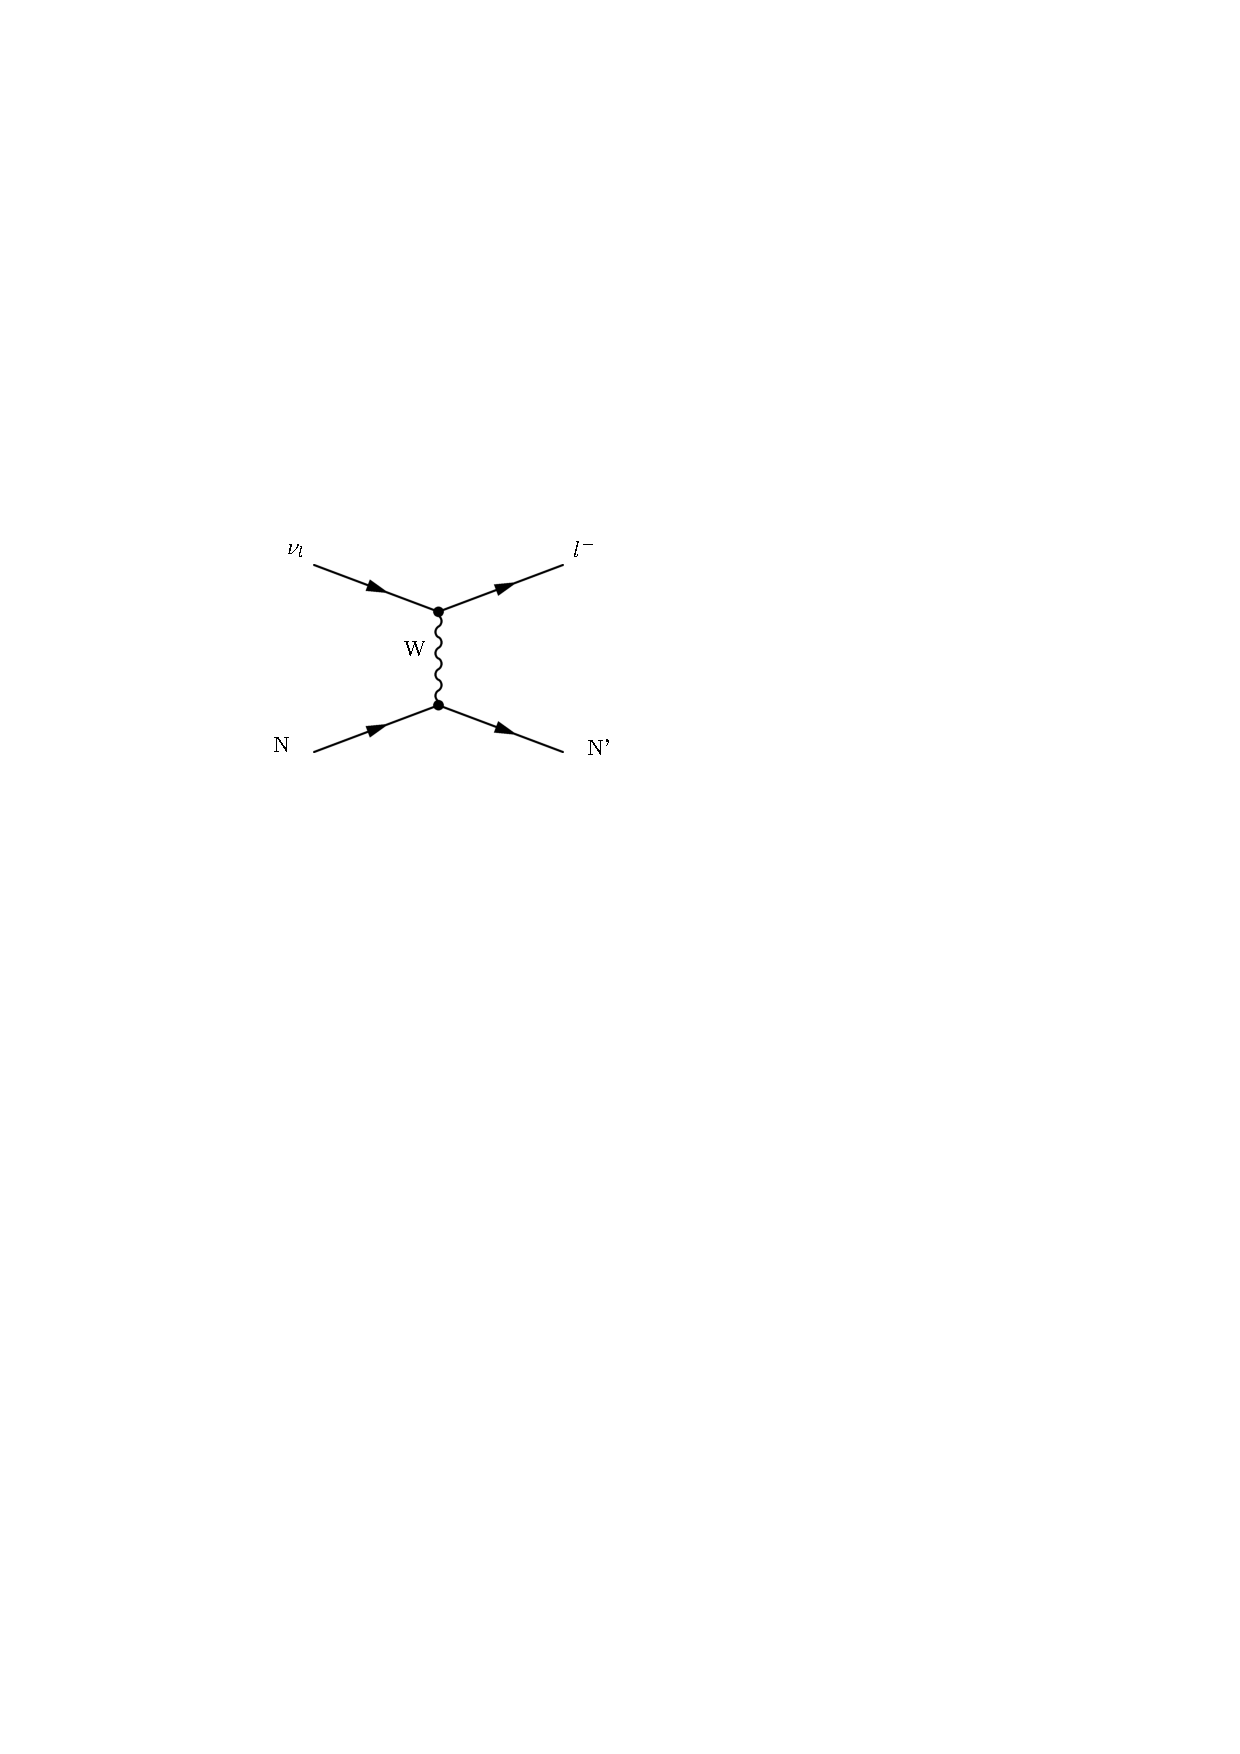
\includegraphics[width=0.65\linewidth]{figures/ccqe_feyn.pdf}
    \caption{Feynman diagram of a charged-current quasi-elastic neutrino-nucleon interaction.}
    \label{fig:ccqe_feyn}
\end{figure}

\item[Resonant and coherent interactions.] In a resonant interaction, the neutrino has enough energy to excite the nucleon to form a resonance, which rapidly decays to a nucleon and one or more mesons while still in the nucleus, as in:
\begin{align}
&\nu_l + p \rightarrow \Delta^{++} \rightarrow l^- + \pi^+ + p \\
&\nu_l + n \rightarrow \Delta^{+} \rightarrow l^- + \pi^+ + n.
\end{align}
This interaction is allowed both by charged current and neutral current exchange.

The GENIE setup used here employs the Rein-Sehgal model \cite{Rein:1980wg} for the resonance production and the Bodek-Ritchie RFG model \cite{Bodek:2011ps} for the interaction of the nucleon within the nucleus. Also in this case, the FSI can cause the absorption of the pion in the nucleus or exchange the charge of the pion.

At low exchanged momentum $Q^2$, pions can be produced also in coherent neutrino-nucleus processes, where the nucleus is left unchanged and a pion is emitted, as shown in the Feynman diagram of Figure \ref{fig:ccoh_feyn}.

\begin{figure}[htbp]
  \begin{subfigure}{0.48\textwidth}
    \begin{center}
    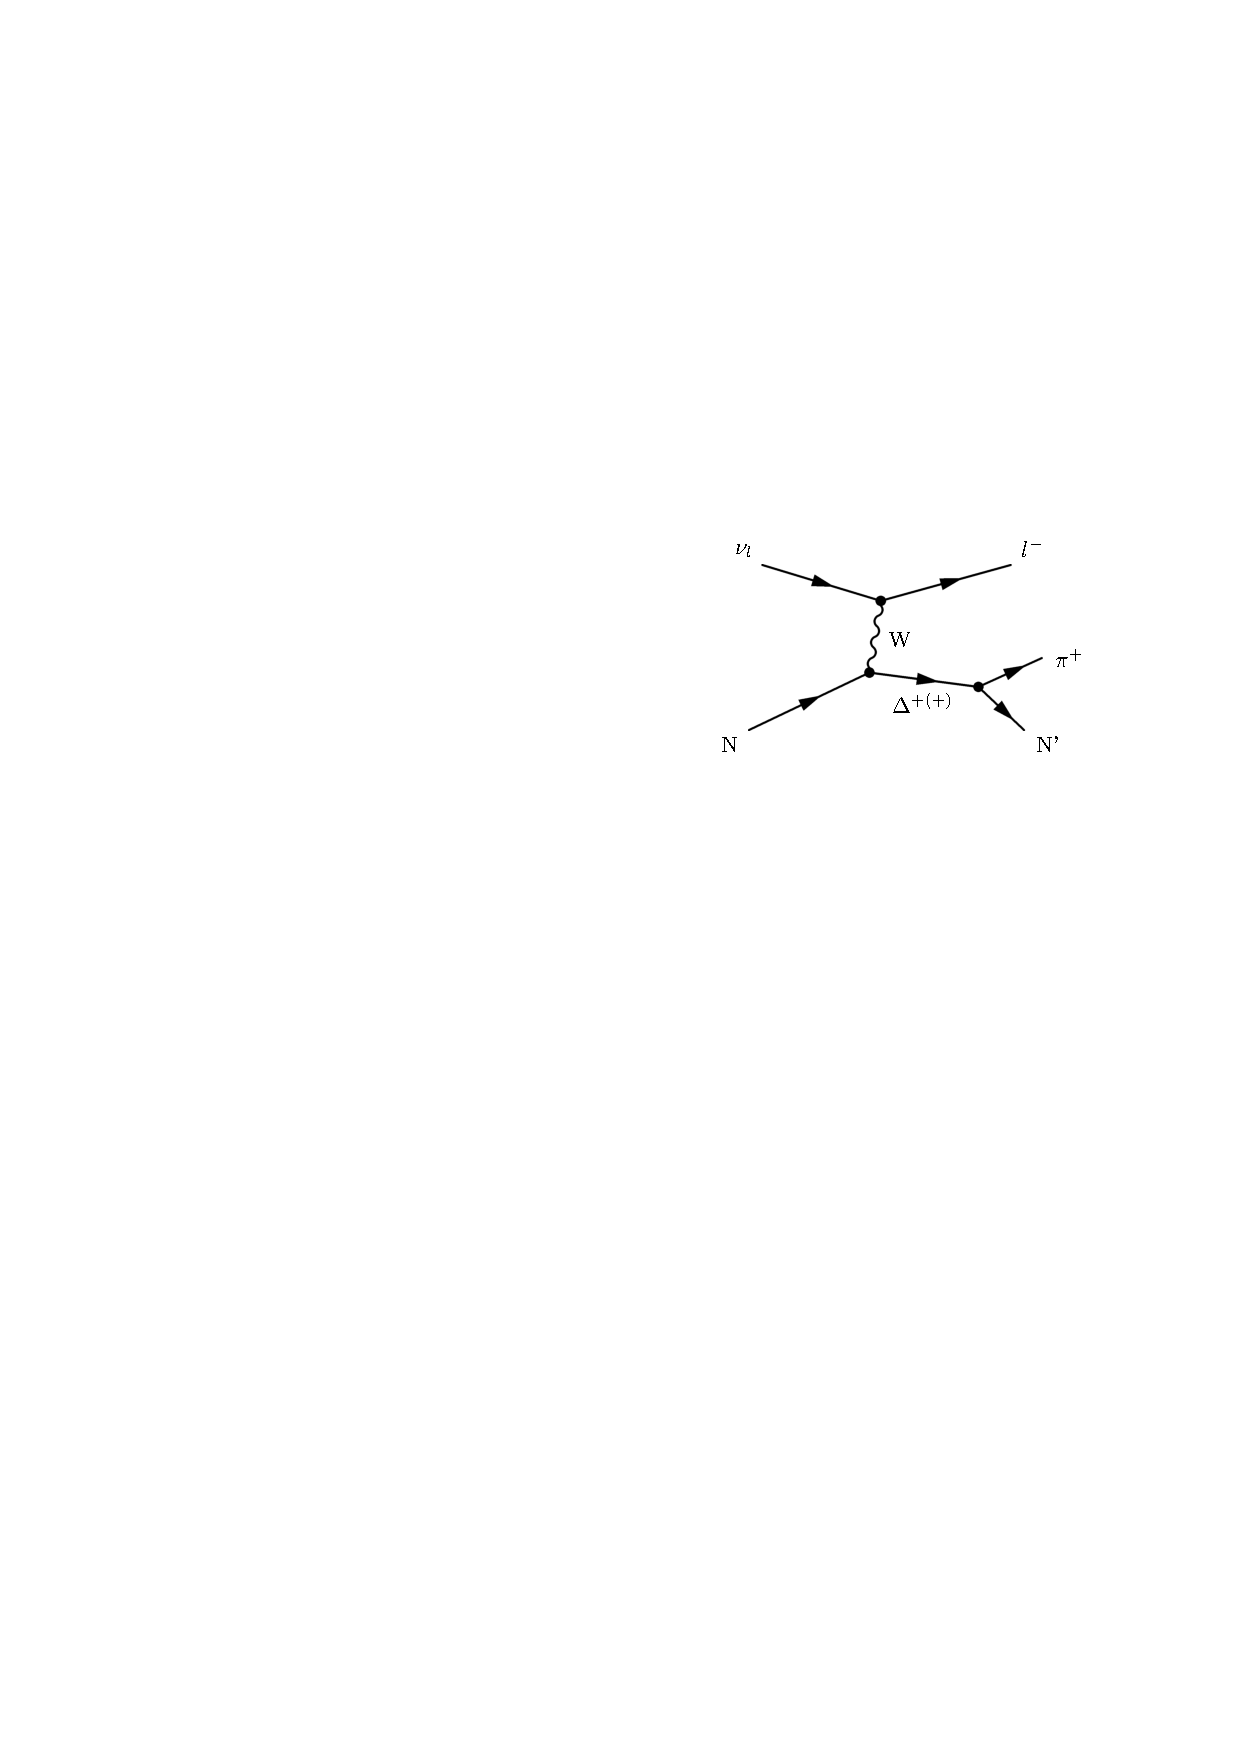
\includegraphics[width=\linewidth]{figures/ccres_feyn.pdf}
    \caption{Charged-current resonant interaction.}
    \label{fig:ccres_feyn}
    \end{center}
  \end{subfigure}\hfill
  \begin{subfigure}{0.48\textwidth}
    \begin{center}
    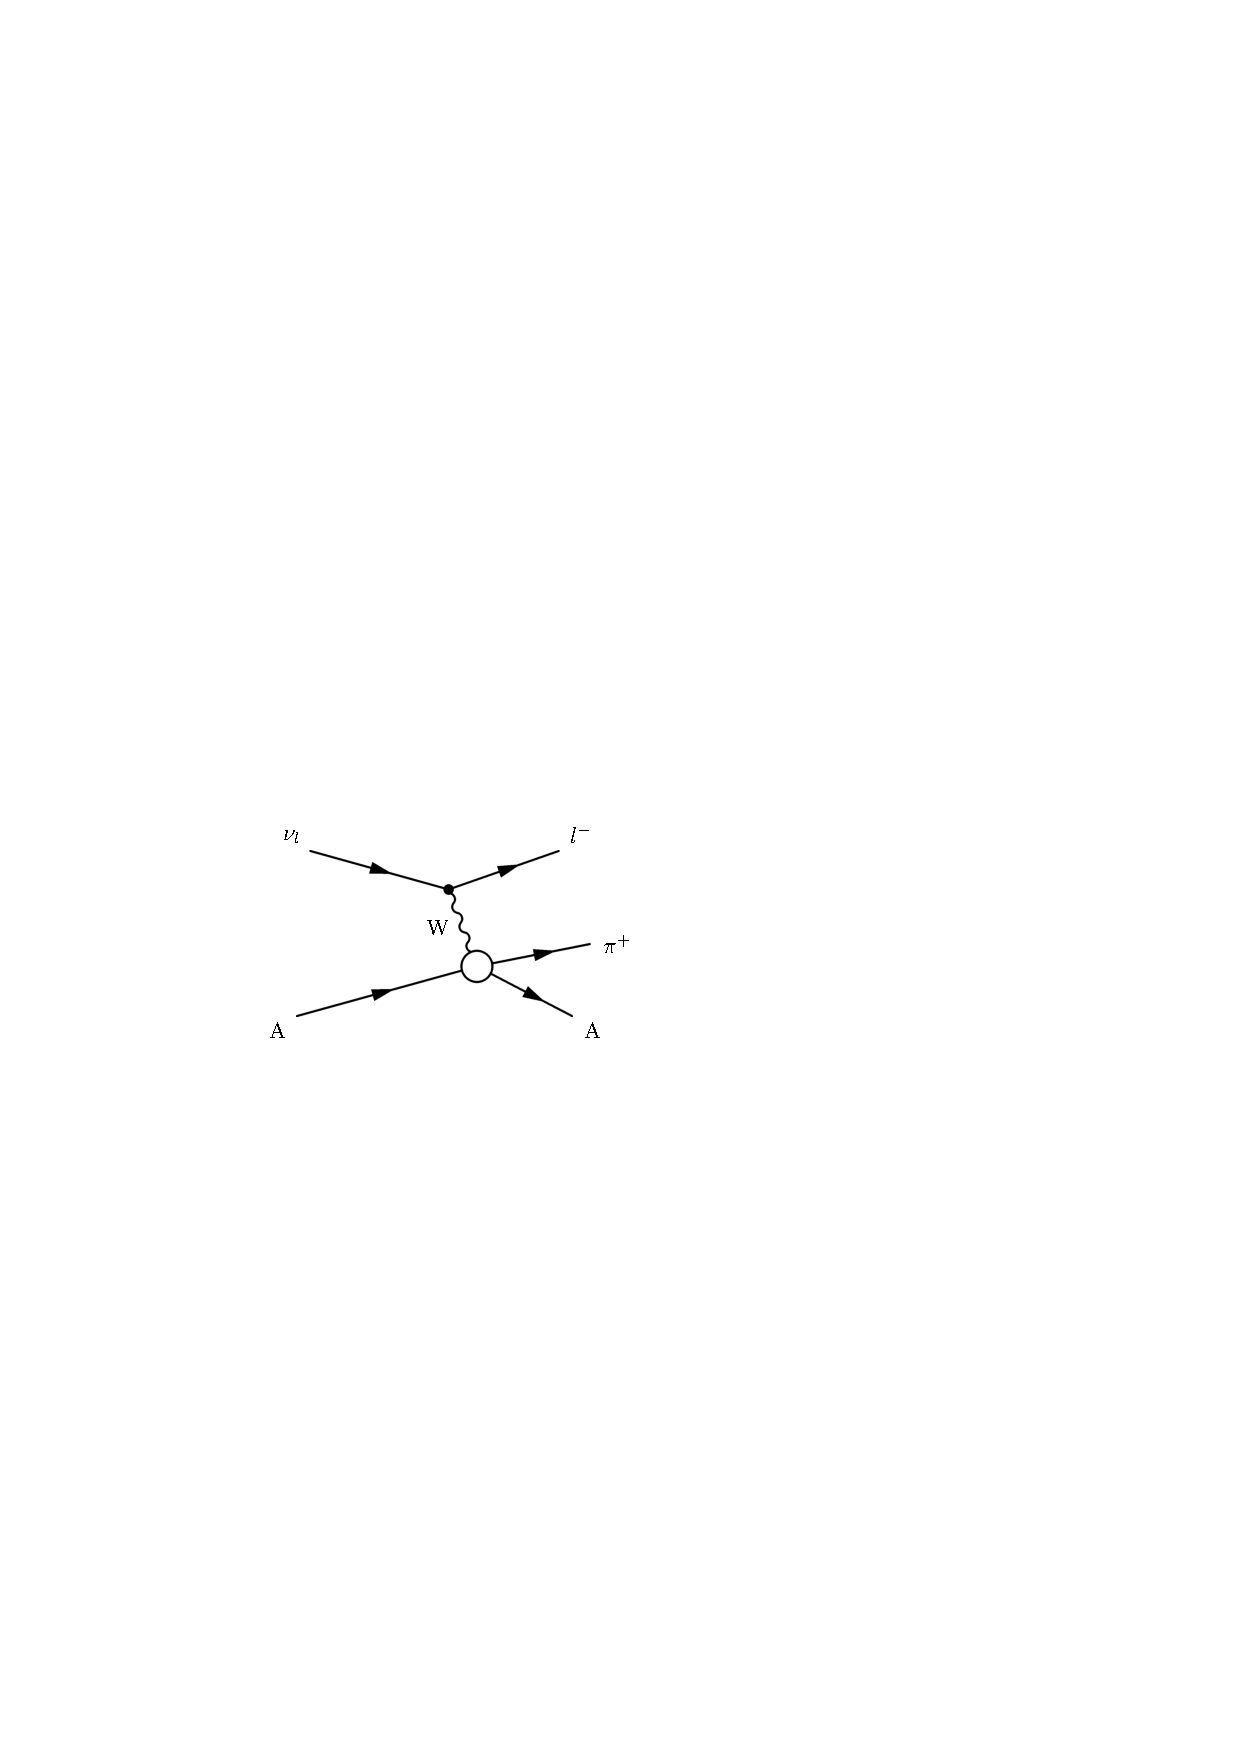
\includegraphics[width=\linewidth]{figures/ccoh_feyn.pdf}
    \caption{Charged-current coherent interaction.}
    \label{fig:ccoh_feyn}
    \end{center}
  \end{subfigure}
  \caption{Feynman diagrams of two neutrino interactions which can produce pions in the final state, charged-current resonant (left) and charged-current coherent (right).}
\end{figure}

\item[Deep inelastic scattering.] In this case, the neutrino has enough energy to interact with the single nucleon components, the quarks, and to break up the nucleus. The result of this interaction often consists in several mesons in the final state. This is the dominant interaction mode for high-energy neutrinos ($>5$~GeV). It is simulated by our setup of GENIE using the Bodek-Yang model \cite{Yang:1998zb}.

Figure \ref{fig:ccdis_feyn} shows the Feynman diagram for this kind of interaction.

\begin{figure}[htbp]
    \centering
    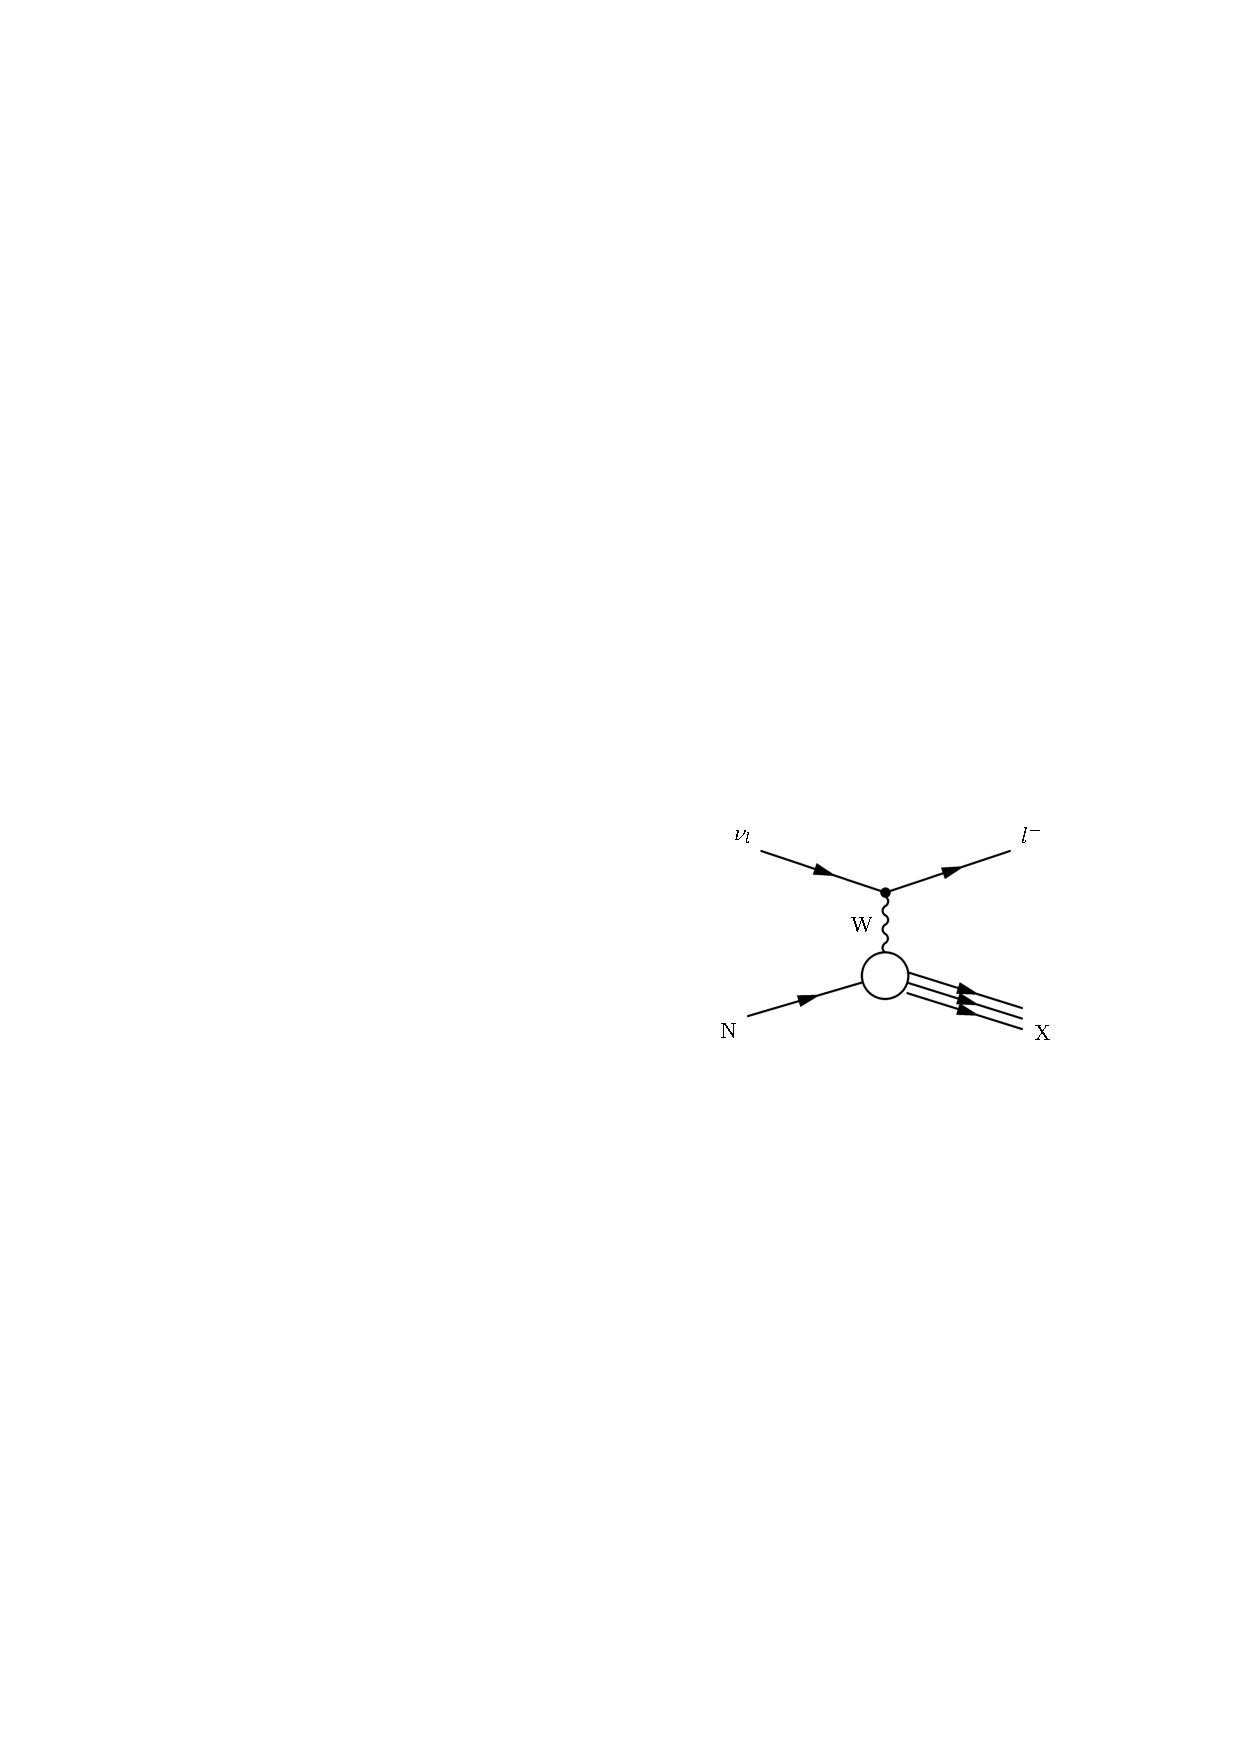
\includegraphics[width=0.65\linewidth]{figures/ccdis_feyn.pdf}
    \caption{Feynman diagram of a charged-current deep inelastic scattering neutrino-nucleon interaction.}
    \label{fig:ccdis_feyn}
\end{figure}


\end{description}

This rich scenario makes the correct reconstruction of neutrino interactions very challenging for any experiment. Usually, oscillations experiments like MiniBooNE (see Section \ref{sec:miniboone}) look for CCQE interactions, whose signature in the detector is easier to identify, but which also require a precise assessment of the final-state interactions.

\section{Future research efforts}
Several experiments have shown compelling evidence for neutrino oscillations, which in turn require non-null neutrino masses. At the moment, massive neutrinos represent the only portal into BSM physics and, for this reason, neutrino physics is one of the most active sectors in particle physics. In the last decade, the parameters of the PMNS mixing matrix of neutrino flavours (see eq. \eqref{eq:pmns}) have been constrained to a precision smaller than 5\%, but some neutrino properties still need to measured. In particular, the CP-violating phase, the neutrino mass hierarchy, and the Majorana or Dirac nature of the neutrino are all research topics actively investigated both by present and future experiments. 

Several experiments are also looking for one of more generations of right-handed neutrinos, which have never been observed and, if existent, would interact only gravitationally and could provide an explanation for the small neutrino masses. Experimentally, they are usually called \emph{sterile neutrinos}.

The following chapters will focus on the search for a low-energy excess of electron neutrinos, which could be a hint of neutrino oscillation into a sterile state. 
\chapter{The LSND and MiniBooNE anomalies}

\minitoc

%This chapter will describe experimental apparatus and the results of the LSND and MiniBooNE experiments.
The LSND experiment observed an excess of $\bar{\nu}_{e}$ in a primarily $\bar{\nu}_{\mu}$ beam in 2001. The MiniBooNE experiment, built to confirm or rule out the anomaly, observed a significant excess of $\nu_{e}$-like ($\bar{\nu}_{e}$-like) events in a primarily $\nu_{\mu}$ ($\bar{\nu}_{\mu}$) beam. Several other neutrino experiments have shown results not fully compatible with the three-flavour scenario and they will be briefly described.  A discussion of the possible physics explanation for the anomalies will also be provided.

\section{The LSND experiment}
The Liquid Scintillator Neutrino Detector (LSND) was an experiment at the Los Alamos National Laboratory which aimed to detect $\bar{\nu}_e$ interactions in a mainly $\bar{\nu}_{\mu}$ beam. The neutrino beam was produced by firing a 800 MeV proton beam into a target, producing charged pions, which were stopped in a beam dump. The $\pi^-$ part was electromagnetically captured by the nucleus, while the $\pi^+$ component initiated the decay chain:
\begin{align}
    \pi^+ \rightarrow & \mu^+\nu_{\mu}\\
    & \rotatebox[origin=c]{180}{$\Lsh$}	 \mu^{+} \rightarrow e^+\bar{\nu}_{\mu}\nu_{e}.
\end{align}
Kinematically, it is possible to distinguish between the neutrino beam produced by decays at rest (DAR), and the neutrino beam produced by decay in flight (DIF). In LSND, this was achieved by looking at events with energies above (below) 60~MeV to select the DIF (DAR) beam, since the maximum energy for a $\bar{\nu}_{\mu}$ produced by a stopping muon is 52.8~MeV ($m_{\mu}/2$) .

The detector was filled with 167 tons of mineral oil (CH$_2$) and doped with 0.031~g/l of organic scintillation material (butyl-PBD).

\begin{figure}[htbp]
    \centering
    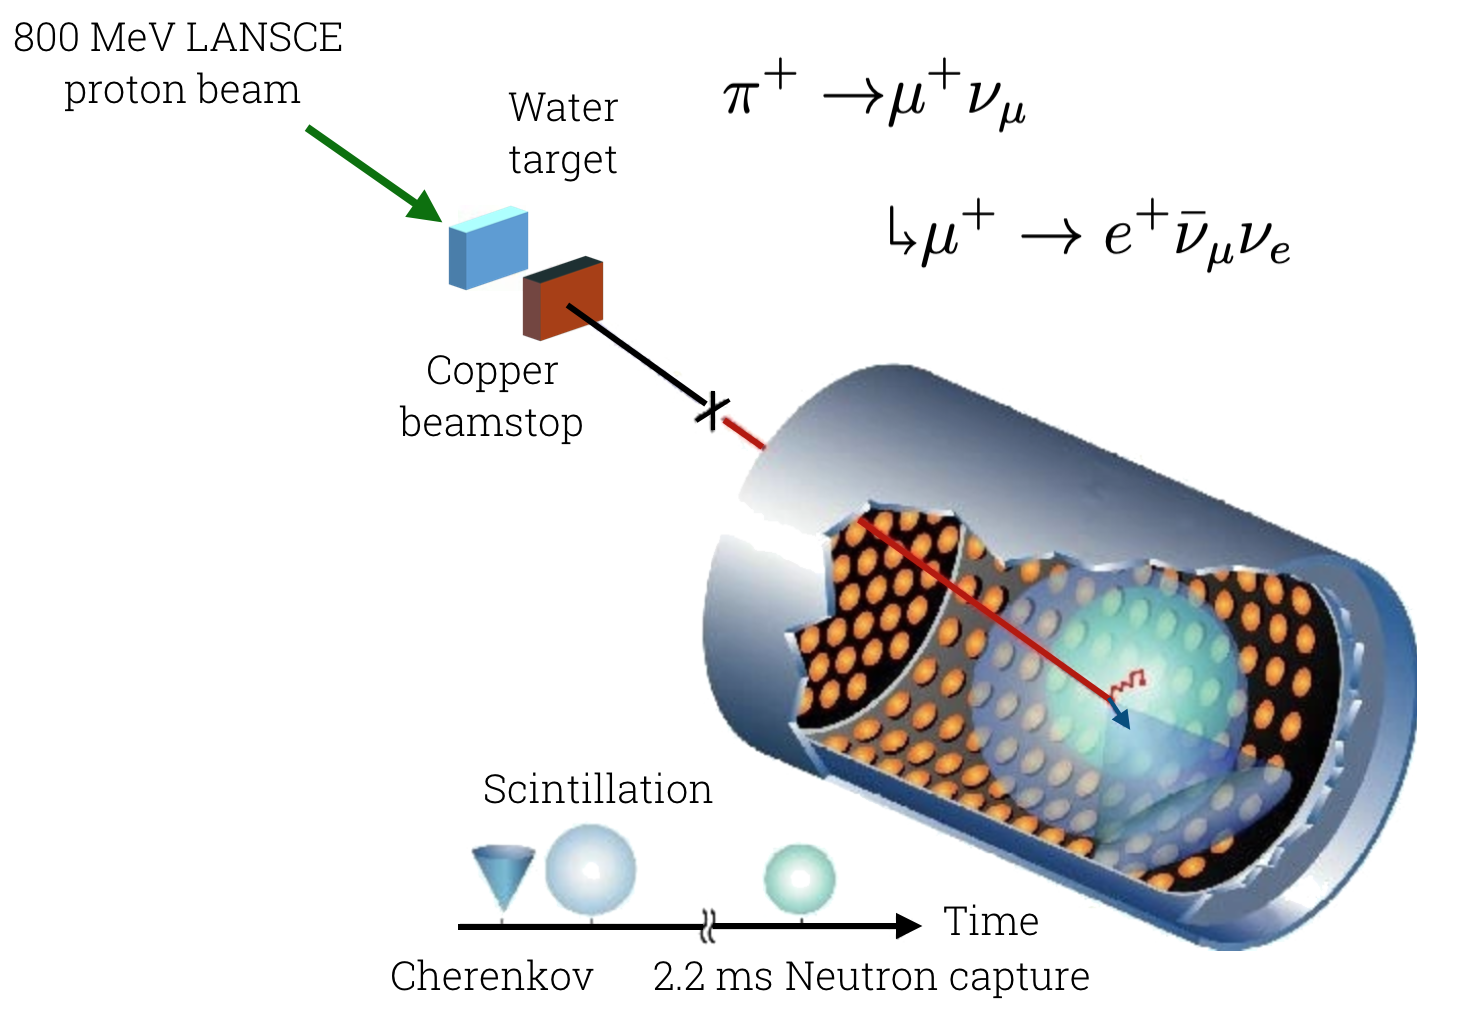
\includegraphics[width=0.9\linewidth]{figures/lsnd_exp.png}
    \caption{A schematic of the LSND experiment and its detection technique: the inverse $\beta$-decay of the neutrinos in the detector produce Cherenkov and scintillation light, in delayed coincidence with the light emitted by the neutron capture.}
    \label{fig:lsnd_exp}
\end{figure}

The $\bar{\nu}_e$ interactions were detected via an inverse $\beta$-decay process and tagged with a delayed coincidence between the positron and the subsequent neutron capture, in a fashion similar to the Cowan and Reines experiment. A schematic of the LSND experiment and its detection technique is shown in Figure \ref{fig:lsnd_exp}.

LSND found an excess of $\bar{\nu}_e$ interactions in the DAR $\bar{\nu}_{\mu}$ beam with a significance of $3.8\sigma$, which could be explained as $\bar{\nu}_\mu$ oscillating into $\bar{\nu}_e$ (Figure \ref{fig:resultlsnd}). Given the $L/E\approx0.75$~m/MeV of the experiment, the mass splitting term obtained with LSND data is $\Delta m_{\mathrm{LSND}}^2\approx1$~eV. This value is one order of magnitude larger than the mass splitting terms obtained with any other reactor, accelerator, atmospheric, or solar experiment \cite{Aguilar:2001ty}. An excess of $\nu_{e}$ was found also in the DIF $\nu_{\mu}$ beam, compatible with the $\bar{\nu}_\mu \rightarrow \bar{\nu}_e$ oscillation result \cite{Athanassopoulos:1997pv}. 

\begin{figure}[htbp]
  \begin{subfigure}{0.45\textwidth}
    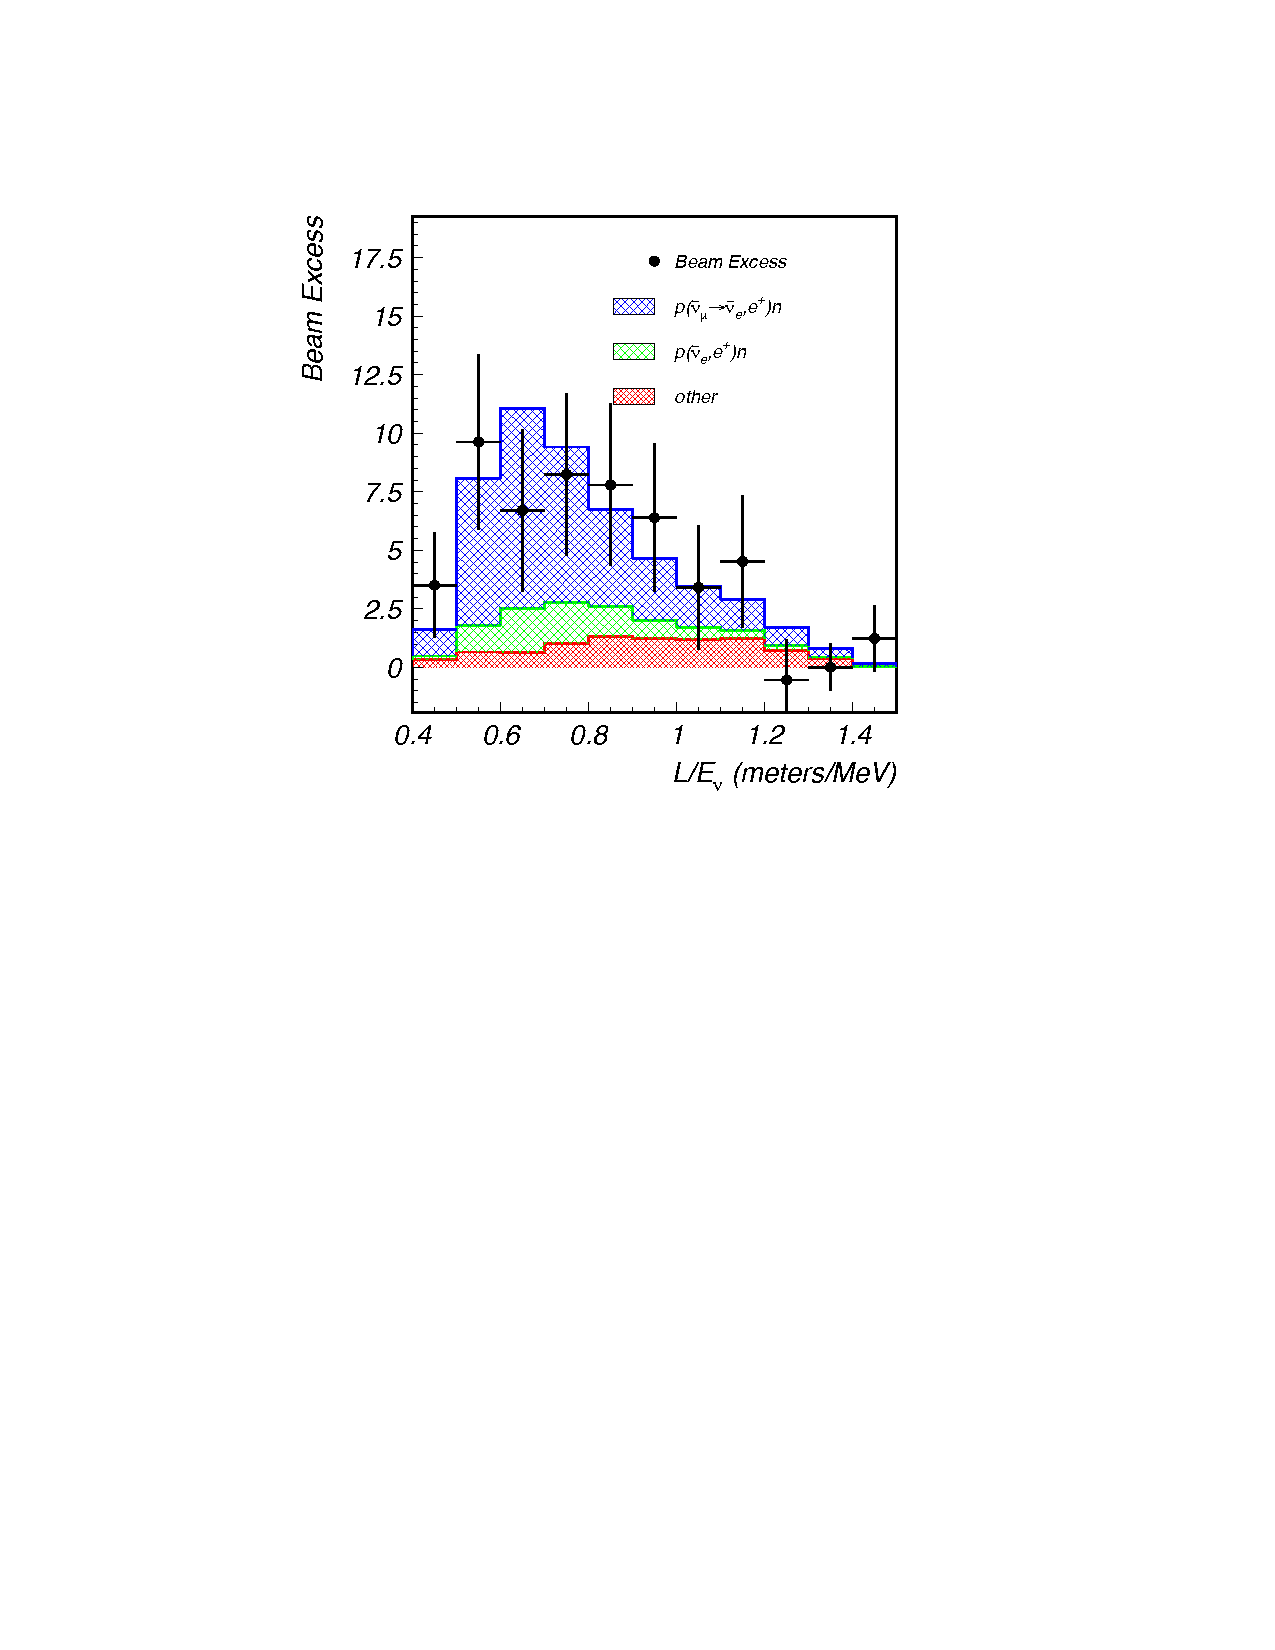
\includegraphics[height=\linewidth]{figures/lsndresult.pdf}
    \caption{$L/E_{\nu}$ distribution for the $\bar{\nu}_{e}$ events in the LSND experiment.}\label{fig:resultlsnd}
  \end{subfigure}\hfill
  \begin{subfigure}{0.45\textwidth}
    \begin{center}
        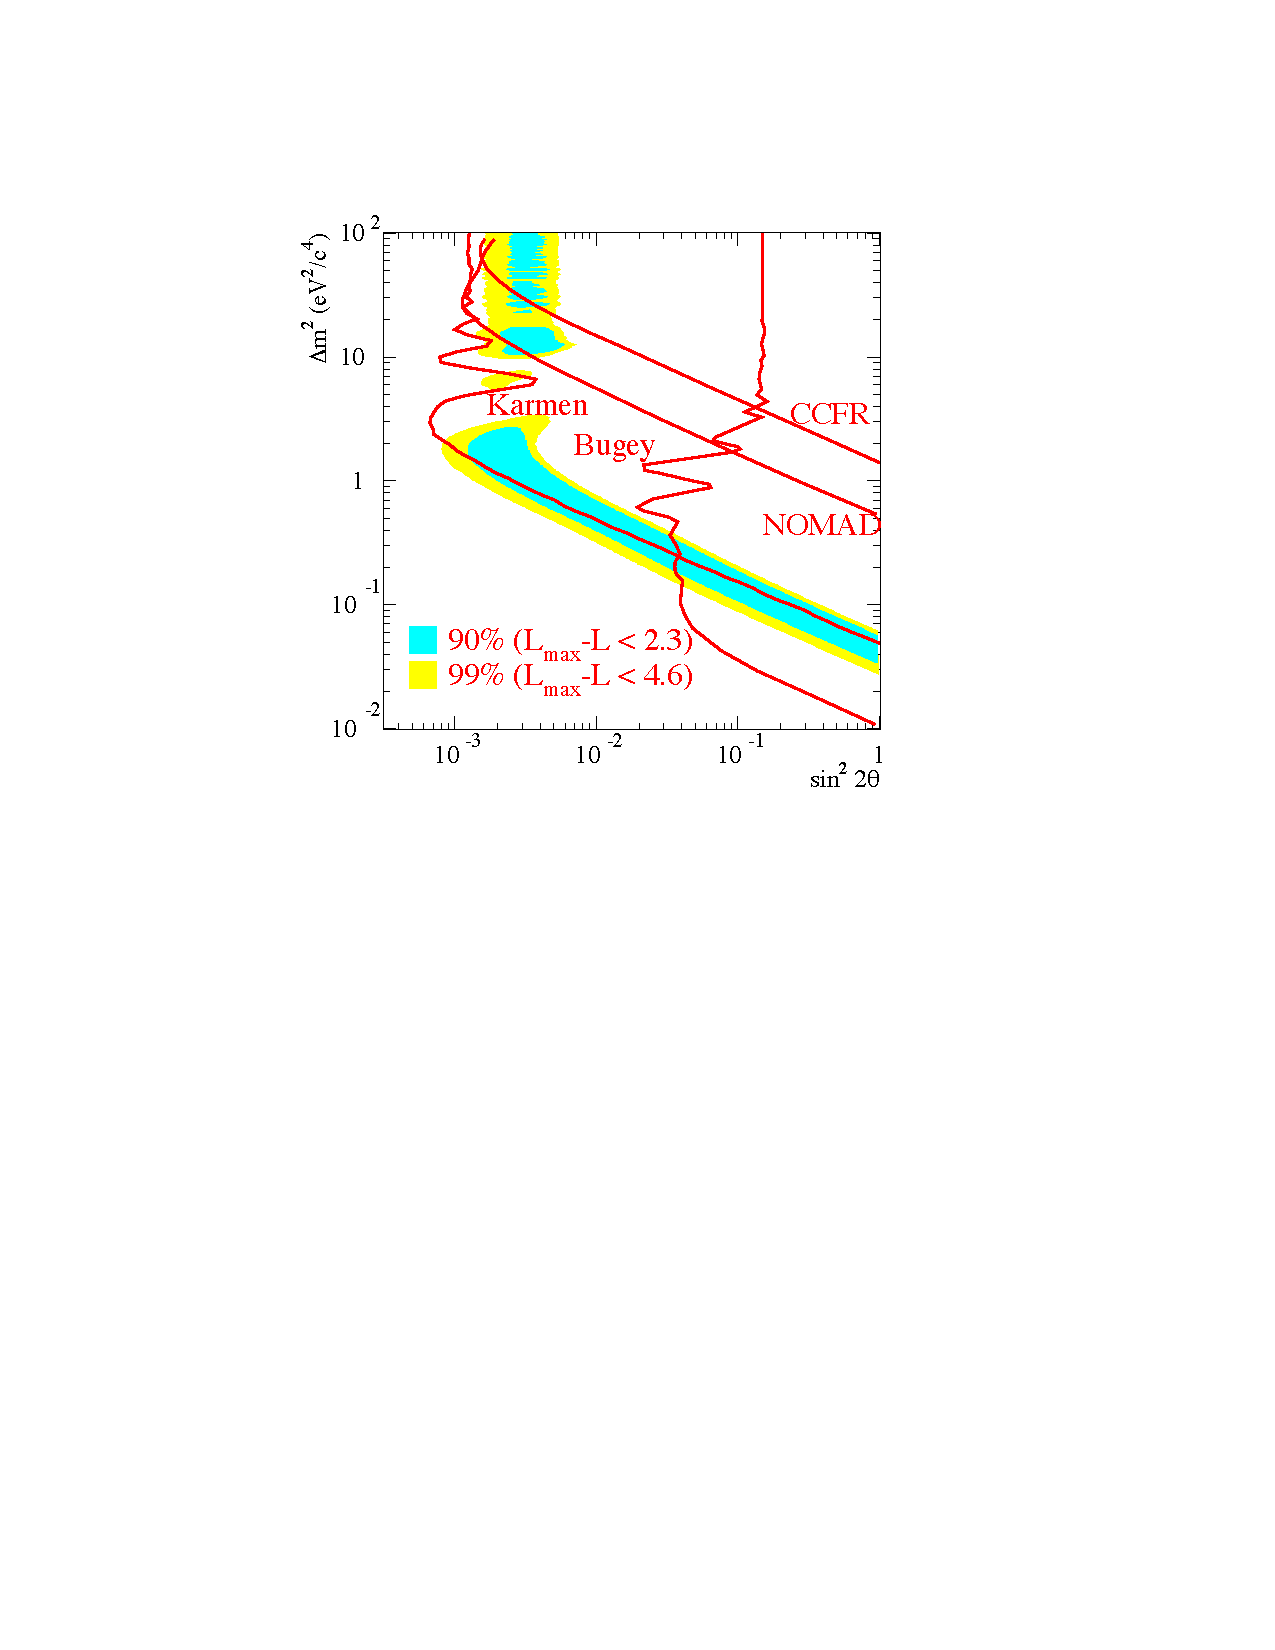
\includegraphics[height=\linewidth]{figures/lsnd_space.pdf}
        \caption{Allowed and excluded regions in the $(\sin^2 2\theta, \Delta m^2)$ parameter space.}\label{fig:lsnd_space}
    \end{center}
  \end{subfigure}
    \caption{The excess of electron antineutrinos observed by the LSND experiment (left) can be interpreted with the presence of a fourth neutrino state. The mixing angles and mass splittings allowed by the LSND data are shown on the right at 90\%~C.L (blue) and 99\%~C.L. (yellow), together with the 90\%~C.L. exclusion limits from other experiments (solid red lines).}
\end{figure}

Figure \ref{fig:lsnd_space} shows the regions in the $(\sin^2 2\theta, \Delta m^2)$ parameter space allowed by the LSND data at 90\%~CL and 99\%~CL. %It is possible to identify two mass-splitting terms and three mixing angles, compatible with a scenario of 3 neutrino flavours, while the LSND allowed region is clearly in a completely different region of the parameter space. 
The KARMEN collaboration employed an experimental setup similar to LSND in order to explore the same region, but it found no significant excess and ruled out a large subset of the LSND parameter space \cite{Eitel:2000by}. 

\section{The MiniBooNE experiment}\label{sec:miniboone}
The MiniBooNE experiment was designed to definitely test the LSND result. It consists of a spherical detector filled with mineral oil and located 541 meters downstream of the Booster Neutrino Beam (BNB) production target at Fermilab. This beam can run both in neutrino mode, producing a mainly $\nu_{\mu}$ beam, and in antineutrino mode, producing a mainly $\bar{\nu}_{\mu}$ beam. The BNB neutrino flux is described in detail by the MiniBooNE collaboration in \cite{AguilarArevalo:2008yp} and will be summarised in Section \ref{sec:beam}. The beam energy is one order of magnitude larger than LSND (8 GeV vs. 800 MeV), but the two experiments have a comparable $L/E_{\nu}$ ratio.

The detector is equipped with 1280 8-inch photomultiplier tubes (PMTs) and employs a separated outer veto region with an extra 240 PMTs for cosmic-ray rejection. Particles interacting in the mineral oil produce Cherenkov light, if above production threshold. The particle identification is based on the different light patterns that each particle produces in the detector: in particular, high-penetrating, heavy particles such as muons will produce sharp rings of Cherenkov light, while lighter particles like electrons and photons will produce fuzzier rings. Neutral pion will instead produce two fuzzy rings partially overlapping when it decays to two photons ($\pi^{0}\rightarrow 2\gamma$). 
This technique introduces an irreducible degeneracy of the particles in the final state, since it is not possible to distinguish a single photon from an electron. 

Energy calibration at MiniBooNE was performed with \emph{in situ} measurements. Cosmic rays, detected with an external hodoscope and stopping in the mineral oil, will produce the typical Michel electron spectrum peaked around $m_{\mu}/2 = 52.8$~MeV. The invariant mass of $\pi^0$ decays can also be reconstructed to measure the energy response around $135$~MeV. 

The oscillation analysis of the MiniBooNE experiment looked for $\nu_e$ charged-current quasi-elastic (CCQE) interactions, where the $\nu_{e}$ exchanges a charged $W$ boson with a neutron in the nucleus, producing an outgoing electron and a proton. This is the dominant interaction type in the sub-GeV region, as shown in Figure \ref{fig:ccqecross}.

However, as outlined in Section \ref{sec:modes}, FSI can alter the particles detected by the apparatus. In particular, CC1$\pi$ events with pion absorption represent a source of uncertainty for a CCQE analysis, since they share the same particles in the final state.

In MiniBooNE, the selected events are called \emph{CCQE-like}, since this definition relies only on the particles in the final state \cite{Katori:2013nca}. 

The energy of the CCQE-like interaction $E_{\nu}^{QE}$ is determined by the electron scattering angle $\theta$ and energy $E_e$, assuming the nucleon at rest, as:
\begin{equation}
    E_{\nu}^{QE} = \frac{2m_n E_e + m_p^2- m_n^2 - m_e^2}{2(m_n - E_e + \cos\theta\sqrt{E_e^2-m_e^2})},\label{eq:ccqe}
\end{equation}
where $m_n$, $m_p$, and $m_e$ are the mass of the neutron, the proton, and the electron, respectively. 
In reality, the nucleon will have a certain Fermi momentum, which will smear out the reconstructed energy. In this case, the estimation of the neutrino energy will depend on the particular model of Fermi motion employed in the simulation, introducing a systematic uncertainty in the measurement.

The presence of events with pion absorption or where the pion escapes the detector introduces as well a distortion in the energy distribution, since the approximation of a 2-body interaction of eq. \ref{eq:ccqe} is no longer valid.


\begin{figure}[htbp]
  \begin{subfigure}{0.48\textwidth}
    \begin{center}
    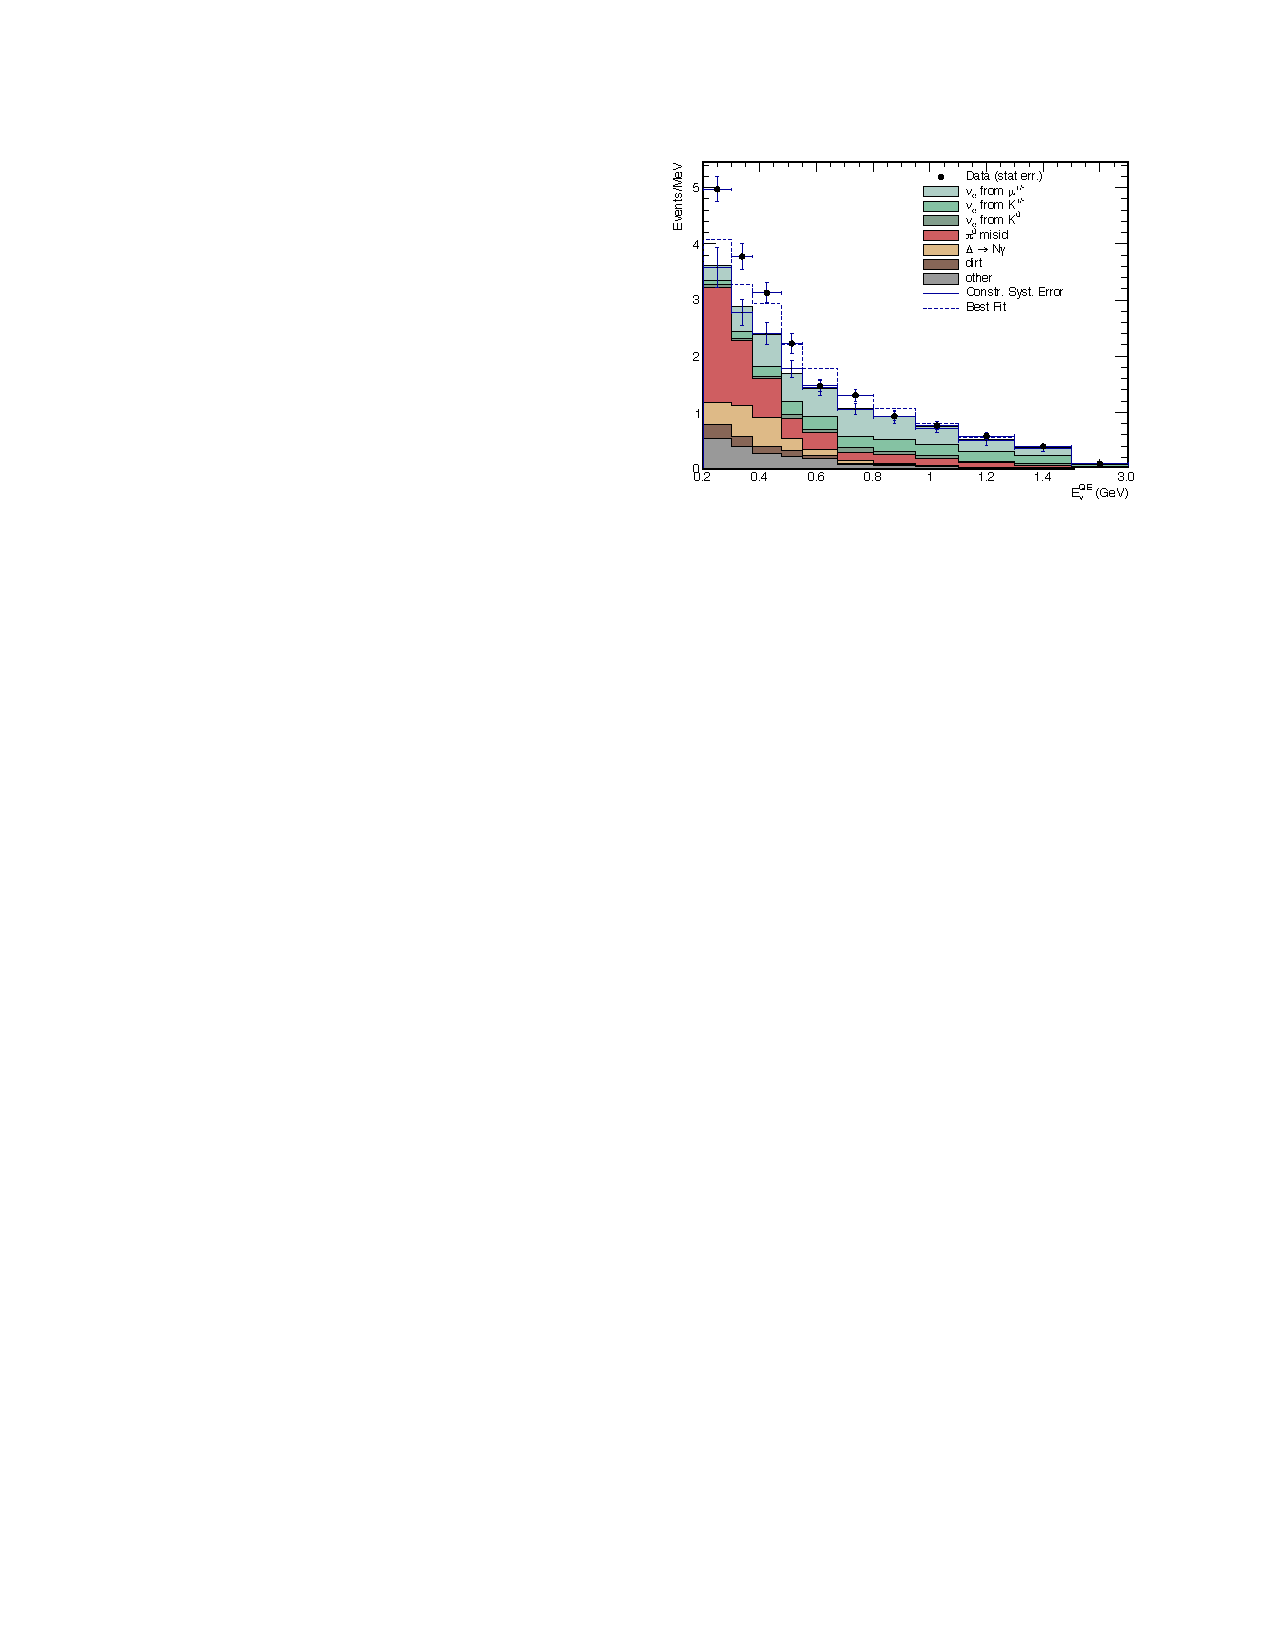
\includegraphics[width=\linewidth]{figures/miniboone_plot.pdf}
    \caption{$E_{\nu}^{QE}$ spectrum in neutrino mode.}
    \label{fig:miniboone_spectrum}
    \end{center}
  \end{subfigure}\hfill
  \begin{subfigure}{0.48\textwidth}
    \begin{center}
    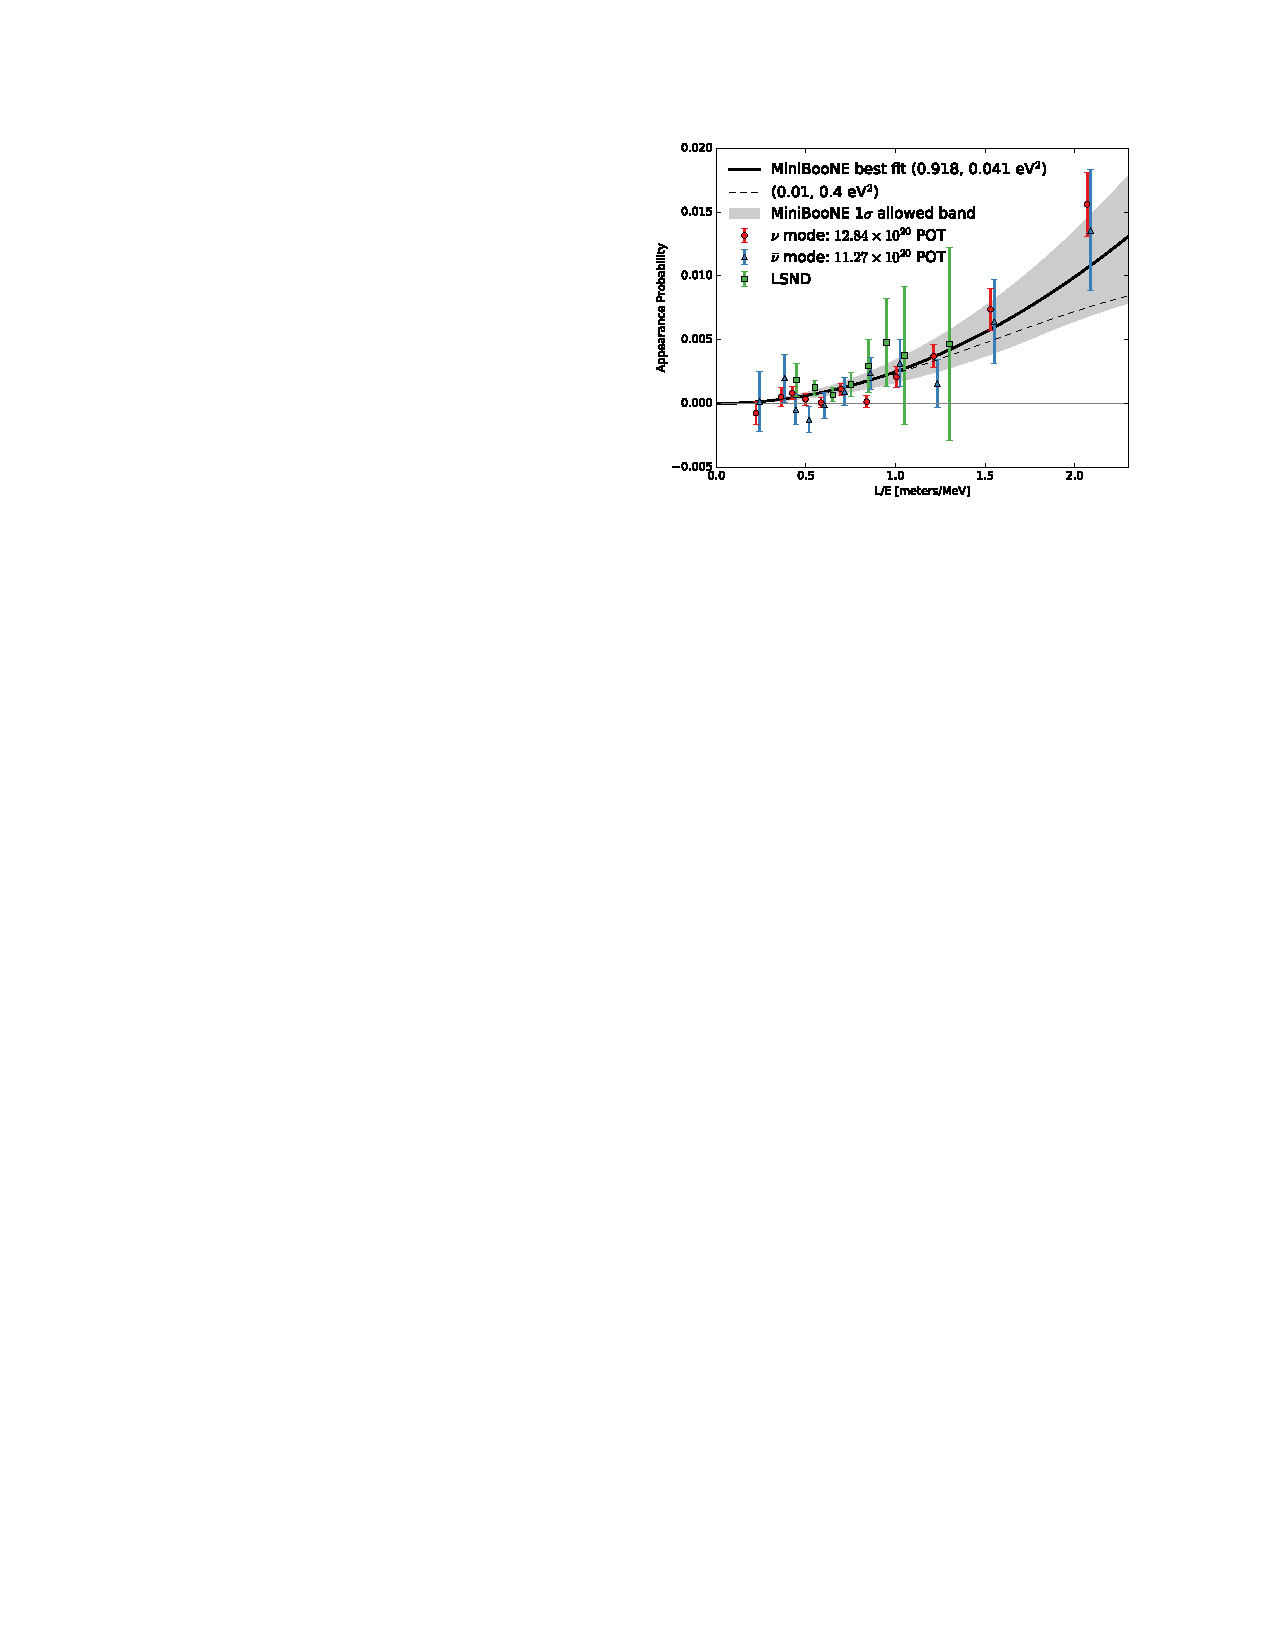
\includegraphics[width=\linewidth]{figures/miniboone_lsnd.pdf}
    \caption{Appearance probability.}
    \label{fig:miniboone_lsnd}
    \end{center}
  \end{subfigure}
  \caption{The MiniBooNE neutrino mode corresponding to the total $12.84\times10^{20}$ POT data, for $\nu_e$ CCQE data (points with statistical errors) and background (histogram with systematic errors). The dashed line represent the two-neutrino model best fit (left). The appearance probability is in agreement with LSND data (right). Adapted from \cite{Aguilar-Arevalo:2018gpe}.}
\end{figure}


The most recent result by the MiniBooNE collaboration \cite{Aguilar-Arevalo:2018gpe} shows a $4.7\sigma$ excess in the combined $\nu_{e}$ and $\bar{\nu}_{e}$ analysis, for $12.84\times10^{20}$ ($11.27\times10^{20}$) POT collected in neutrino (antineutrino) mode. The observed excess of data events is $460.5 \pm 99.0$. The energy spectrum of the $\nu_E^{\mathrm{CCQE}}$ selected events in neutrino mode is shown in Figure \ref{fig:miniboone_spectrum}. The analysis followed a blind approach, where the data sub-sample containing the signal events, defined requiring a single isolated electron in the detector, was not opened until the analysis tools and the simulation were well understood. 

The $\nu_{e}$ oscillation was measured with a combined fit of the $\nu_{e}$ and $\nu_{\mu}$ selected events. This approach, which will be employed also by the MicroBooNE experiment, allows to measure more precisely the neutrino flux: in this way, the $\nu_e$ candidates from $\nu_{\mu}$ oscillation cannot be interpreted as an underestimation of the total neutrino flux, since this would show up as a disagreement in the number of $\nu_{\mu}$ events as well. A measurement of the $\nu_{\mu}$ component of the flux allows also to partially constrain the number of intrinsic $\nu_e$, since around half of them are produced in the decay:
\begin{align}
    \pi^+ \rightarrow & \mu^+\nu_{\mu}\\
    & \rotatebox[origin=c]{180}{$\Lsh$}	 \mu^{+} \rightarrow e^+\bar{\nu}_{\mu}\nu_{e}.
\end{align}

The excess of data events is in the sub-GeV energy region and consistent in energy and magnitude with the LSND result. The two excess combined gives a significance of $6.0\sigma$. Figure \ref{fig:miniboone_lsnd} shows the agreement of the appearance probability as a function of the $L/E$ distribution for LSND and MiniBooNE. 

\subsection*{MiniBooNE backgrounds}
The background events of the MiniBooNE experiment can be divided into four main categories:
\begin{description}
    \item[Intrinsic $\nu_e$.] The $\nu_e$ component of the beam, coming from $\mu^{\pm}$, $K^{\pm}$, and $K^0$, is the irreducible background of the experiment, since it can't be distinguished from $\nu_{\mu}$ oscillating into $\nu_{e}$. This component of the flux is partially constrained by measuring the $\nu_{\mu}$ interactions.
    \item[Misidentified $\pi^0$.] The background from misidentified $\pi^0$ events represents the largest component. These events are particularly challenging to reconstruct, since very forward-boosted photons will appear in the detector as a single fuzzy ring. The MiniBooNE collaboration has constrained this contribution by reconstructing the invariant $\pi^0$ mass of the event and obtaining a sample with a purity $>90\%$ of NC $\pi^0$ events. The total uncertainty on the NC background is 7\% \cite{Karagiorgi:2010zz}.
    \item[Misidentified $\Delta\rightarrow N\gamma$.] A neutral current resonant interaction can produce a a $\Delta$ resonance, which has a rare electromagnetic decay channel $\Delta\rightarrow N\gamma$, where $N=n,p$. This channel is also constrained by the NC $\pi^0$ \emph{in situ} measurement, times the small branching ratio  $(0.56\pm0.04)\%$. The uncertainty on this component is 12\%.
    \item[Dirt.] The dirt background, meaning neutrino interactions happening outside the detector but where at at least one particle in the final states interacts inside, is also constrained with an \emph{in situ} measurement, where events reconstructed close to the detector boundaries and pointing inwards are selected. 
\end{description}

Both the $\pi^0$ and the $\Delta\to N\gamma$ backgrounds come from the inability of a Cherenkov detector to distinguish between photons and electrons, which is instead one of the most powerful capabilities of a LArTPC, as it will be described in detail in Section \ref{sec:detector}. MiniBooNE is also not able to distinguish between negative and positive charged particles, making it impossible to distinguish neutrino and antineutrino events.

Non-beam backgrounds (such as cosmic rays) are removed by requiring light in the detector in time with the BNB spill of 1.6~\si{\micro}s and no activity in the outer veto volume, achieving a 99.99\% rejection efficiency. 
In order to reject the beam-related background events, the MiniBooNE collaboration employed an electron-muon likelihood cut, an electron-pion likelihood cut, and a cut on the invariant $m_{\gamma\gamma}$ mass.

The average selection efficiency for $\nu_e^{\mathrm{CCQE}}$ events is $\sim20$\% \cite{Aguilar-Arevalo:2018gpe}.

\subsection*{Possible interpretations of the LSND and MiniBooNE results}

A proposed solution to the LSND anomaly is to have one sterile additional neutrino state, which would mix with the standard three neutrinos, in a 3+1 scenario. The PMNS matrix in this case will have an extra dimension ($4\times4$) and the sterile mass neutrino eigenstate will be written as:
\begin{equation}
    \ket{\nu_s}=\sum^{3+1}_{\alpha}U_{i,\alpha}\ket{\nu_{\alpha}}.
\end{equation}
A diagram of the mass hierarchy in this scenario is shown in Figure \ref{fig:masslsnd}.

\begin{figure}[htbp]
    \centering
    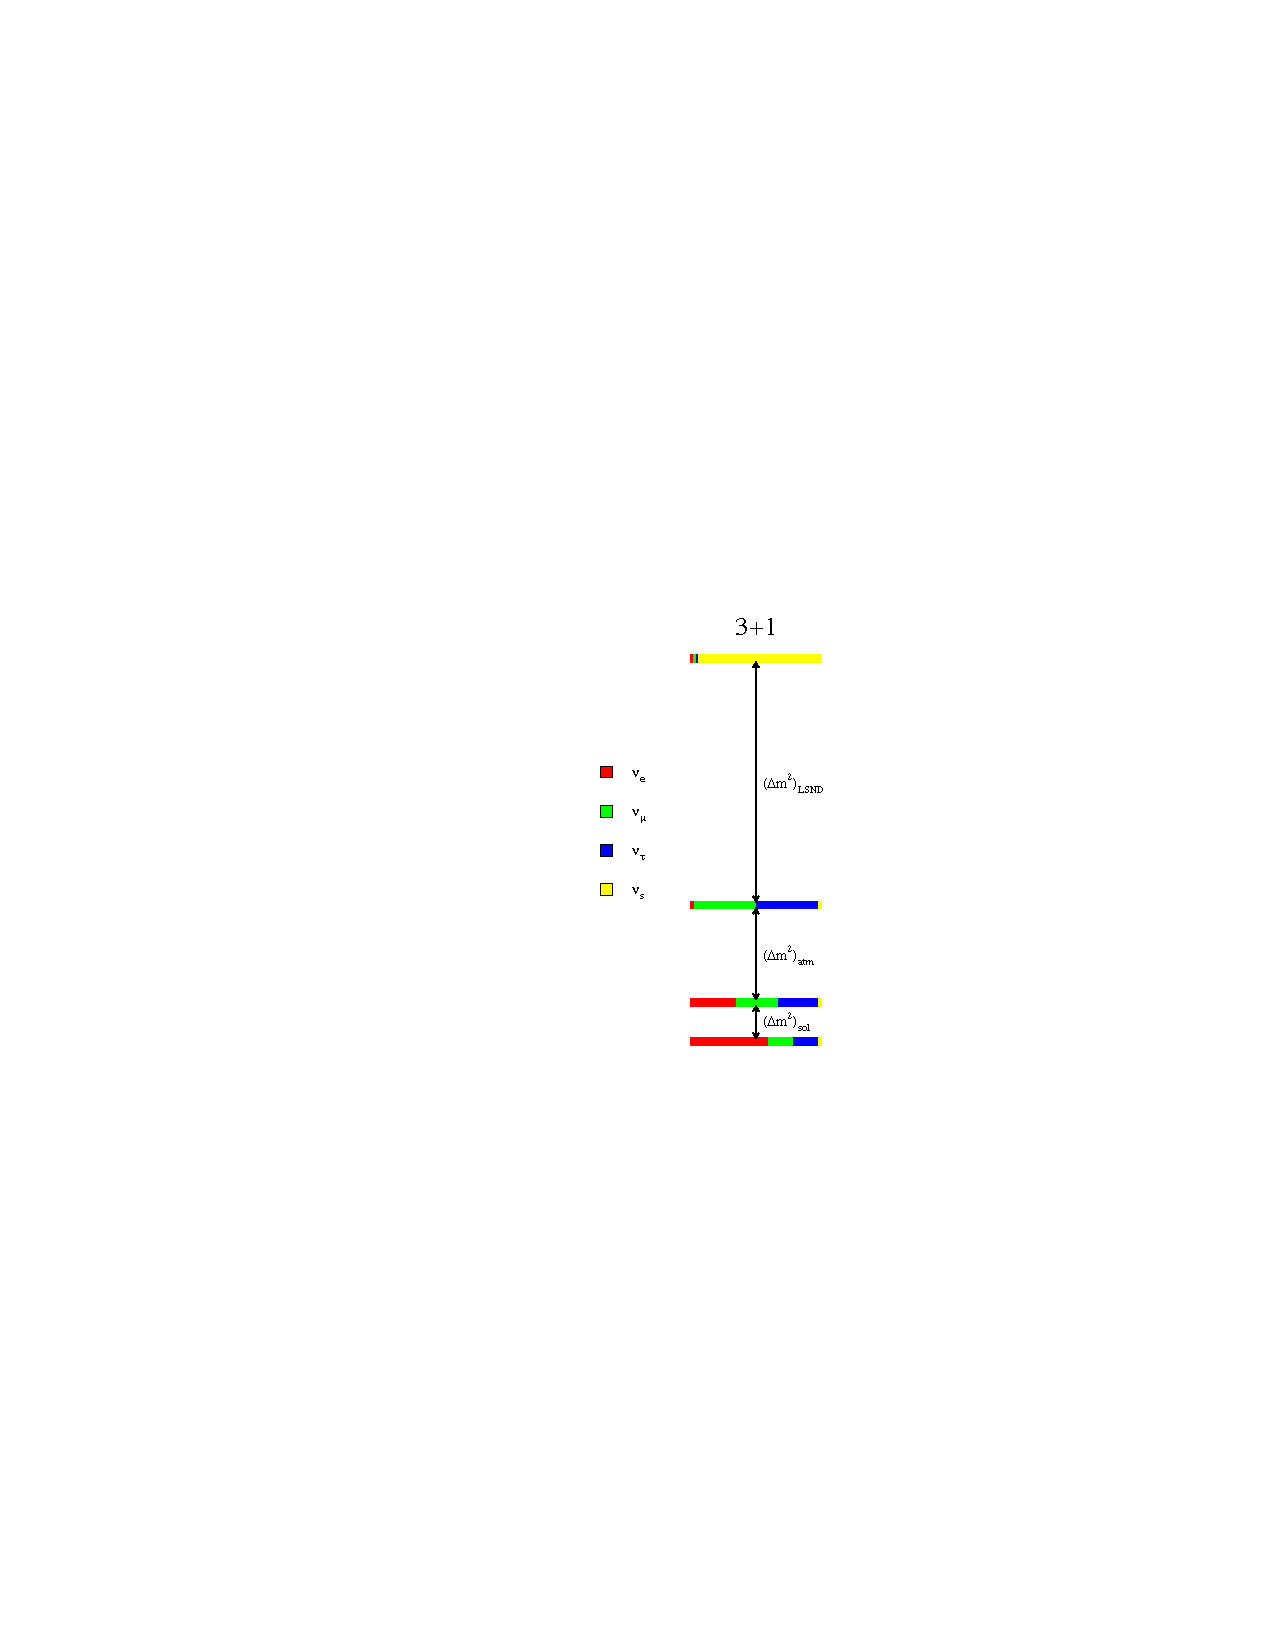
\includegraphics[width=0.3\linewidth]{figures/masslsnd.pdf}
    \caption{Neutrino mass normal hierarchy in the scenario of 3+1 neutrinos (from \cite{deGouvea:2004gd}).}
    \label{fig:masslsnd}
\end{figure}

As shown in Figure \ref{fig:miniboone_lsnd}, the LSND excess seems to be in agreement with the results of the MiniBooNE experiment, both in neutrino and antineutrino mode. The MiniBooNE collaboration was able to constrain all the simulated experimental backgrounds with \emph{in situ} measurements. The excess must then come from an unexpected background source or from BSM interactions, such as the existence of one or more sterile neutrinos.
Figure \ref{fig:miniboone_bestfit} shows the MiniBooNE allowed regions in neutrino and antineutrino mode for the two-neutrino oscillation model. The best fit point, however, is disfavoured by the OPERA $\nu_{e}$ appearance analysis \cite{Agafonova:2018dkb}.

\begin{figure}[htbp]
    \centering
    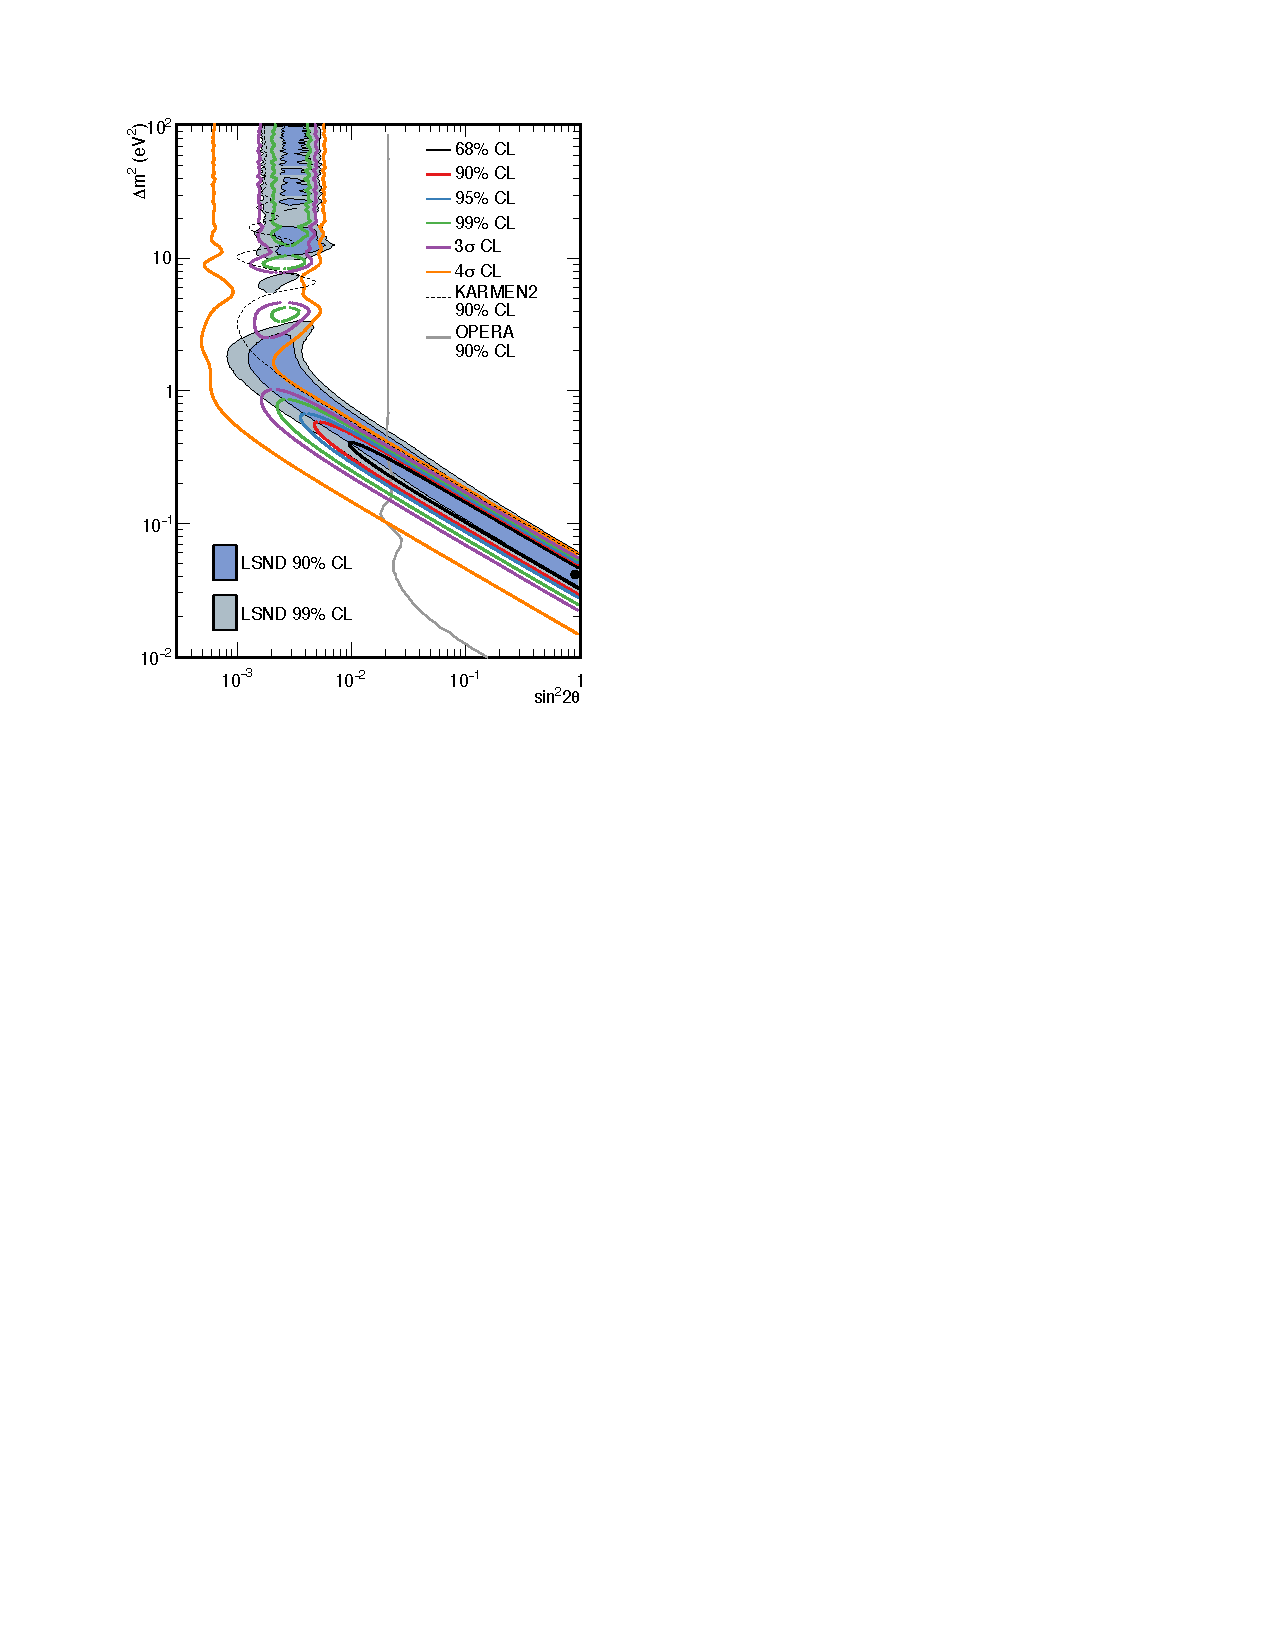
\includegraphics[width=0.7\linewidth]{figures/miniboone_bestfit.pdf}
    \caption{MiniBooNE allowed regions for the combined neutrino mode and antineutrino for events with $200<E_{\nu}^{QE}<3000$~MeV within a two-neutrino oscillation model. The black point at $( \sin^22\theta, \Delta m^2)=(0.96, 0.041~\mathrm{eV^2})$ represents the best fit \cite{Aguilar-Arevalo:2018gpe}.}
    \label{fig:miniboone_bestfit}
\end{figure}


\section{Oscillations anomalies: the global picture}
The global fit of neutrino oscillations experiments in the 2-neutrino approximation (so using Eq. \ref{eq:prob} and Eq. \ref{eq:prob2}) is shown in Figure \ref{fig:globalfit}. Atmospheric, solar, and reactor experiments roughly overlap in three regions in the $(\tan^2\theta, \Delta m^2)$ space, giving three mixing angles and two mass splittings values, as expected in a 3-flavour scenario. 

\begin{figure}[htbp]
    \centering
    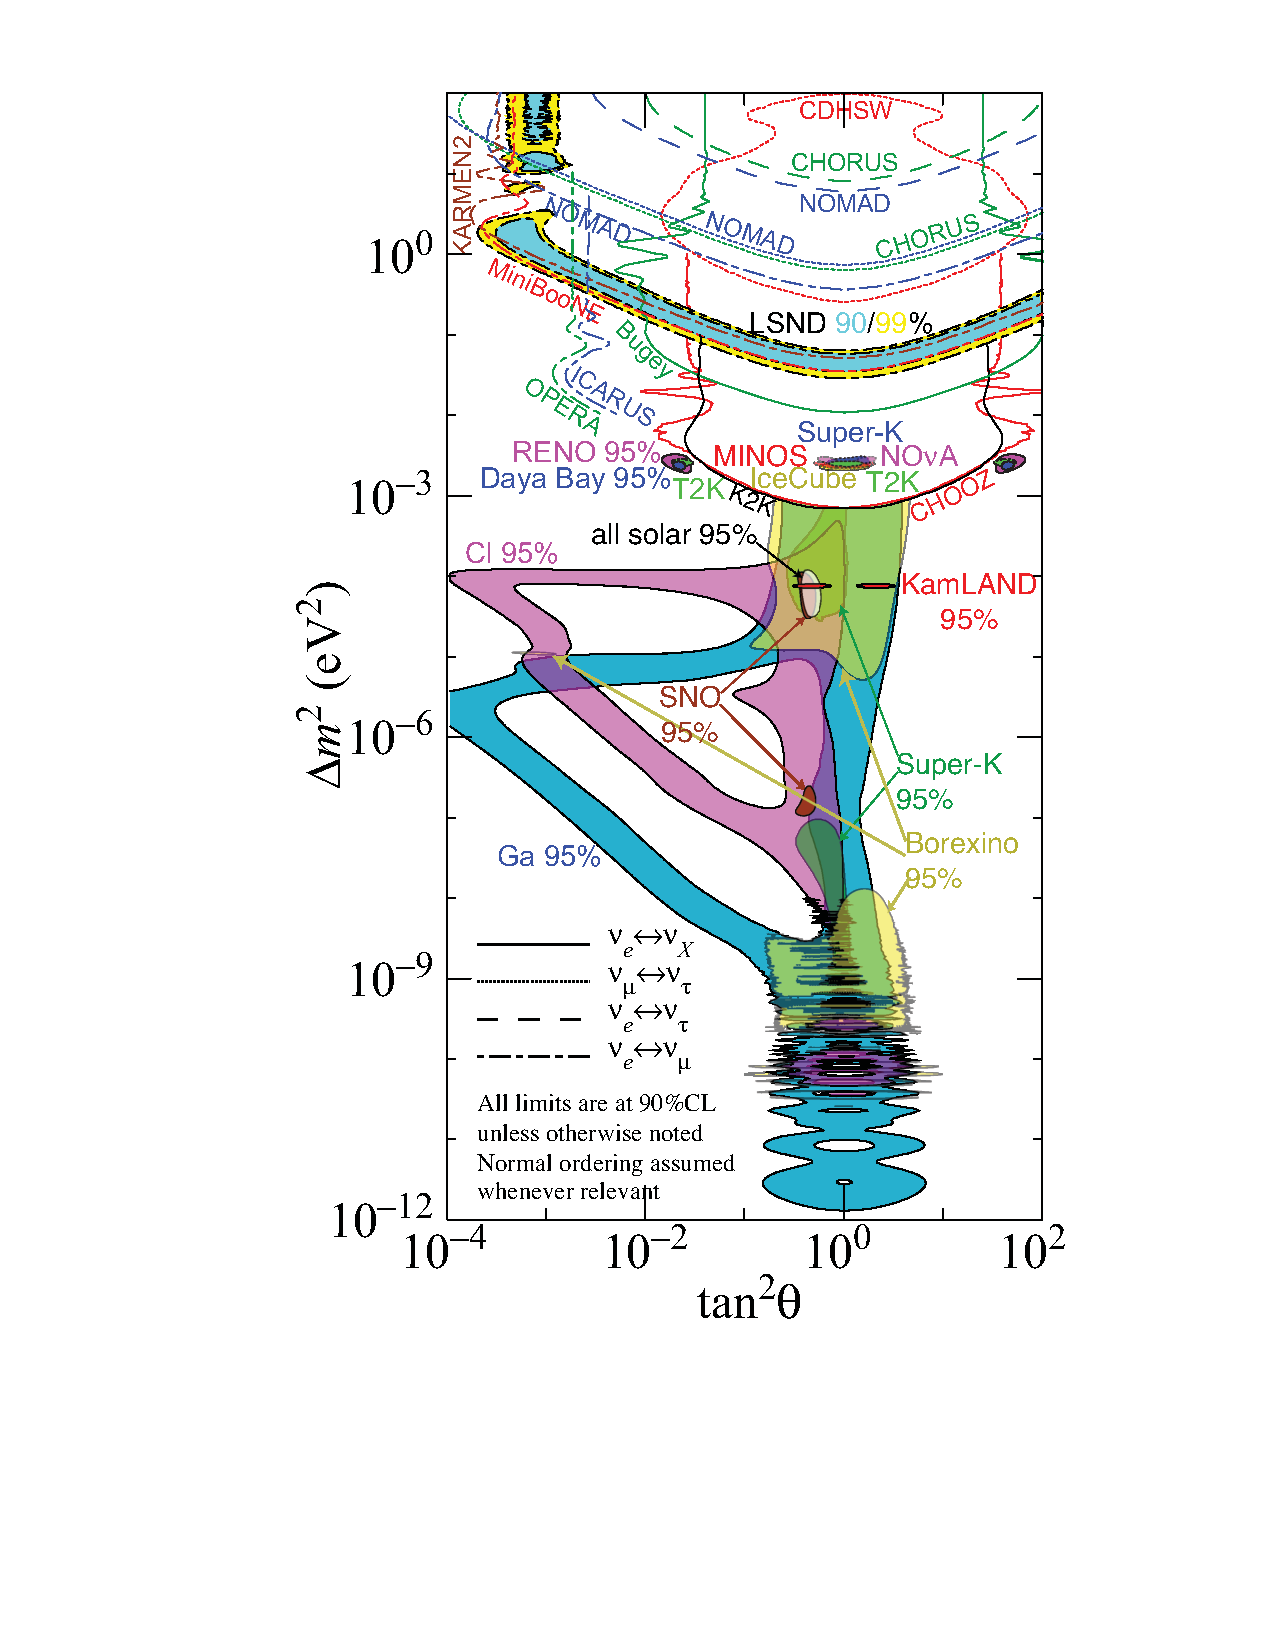
\includegraphics[width=0.7\linewidth]{figures/globalfit.pdf}
    \caption{The squared-mass splittings and mixing angles favoured (solid regions) or excluded (open regions) by existing neutrino oscillation measurements. Results are categorised by channels: $\nu_e$ disappearance (solid lines), $\nu_{\mu} \leftrightarrow \nu_{\tau}$  (dotted lines), $\nu_{e} \leftrightarrow \nu_{\tau}$ (dashed lines), and $\nu_{e} \leftrightarrow \nu_{\mu}$ (dashed-dotted lines). The normal mass ordering is assumed where relevant. Taken from \cite{PhysRevD.98.030001}. Does not include MiniBooNE latest result \cite{Aguilar-Arevalo:2018gpe}.}
    \label{fig:globalfit}
\end{figure}

However, LSND and MiniBooNE results do not agree with the allowed regions, since their mass splitting term is much larger ($\Delta m^2 \sim 1~$eV$^2$). Moreover, they are not the only two experiments which have observed anomalies in the neutrino sector. Several other experiments obtained results not completely in agreement with the theoretical expectations. In particular, it is possible to identify two categories of anomalies, classified according to the experimental technique employed: inverse beta decay from solar neutrinos of gallium into germanium (\emph{radiochemical experiments}) and inverse beta decay from reactor neutrinos (\emph{reactor experiments}).

\subsection{Radiochemical experiments}
    The GALLEX experiment at Gran Sasso and the SAGE experiment at Baksan employed a detection technique similar to the one of Ray Davis experiment at Homestake. In this case, solar neutrino interactions were detected through inverse $\beta$ decay of $^{71}$Ga atoms into $^{71}$Ge (instead of $^{37}$Cl into $^{37}$Ar):
\begin{equation}
    \nu_e + ^{71}\mathrm{Ga} \rightarrow e^- + ^{71}\mathrm{Ge}.
\end{equation}
The energy threshold for this reaction is 233~keV, which allows to observe the neutrino interactions produced in the solar $pp$ chain reaction (see Figure \ref{fig:solar}). Both experiments employed intense radioactive materials for calibration. GALLEX used a $^{51}$Cr source, while SAGE used $^{51}$Cr and $^{37}$Ar. These two sources decay via electron capture, emitting an electron neutrino:
\begin{equation} 
    ^{A}_{Z}\mathrm{X} + e^{-} \rightarrow ^{A}_{Z-1}\mathrm{Y} + \nu_{e}.
\end{equation}

The two experiments observed a deficit of $\nu_{e}$ interactions in all the three cases, which favours with $2.7\sigma$ significance the hypothesis of short-baseline neutrino oscillation \cite{Giunti:2010zu}.

\begin{figure}[htbp]
  \begin{subfigure}{0.48\textwidth}
    \begin{center}
    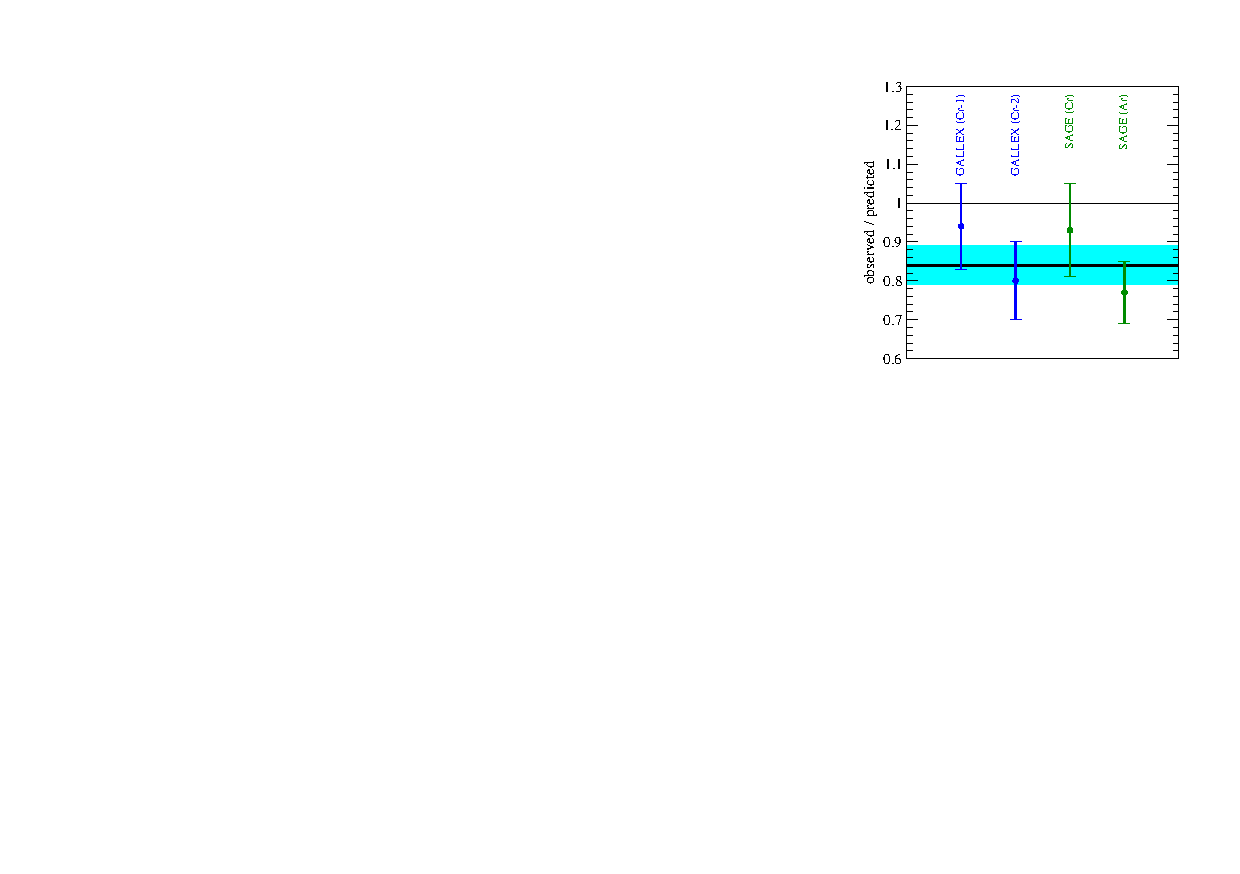
\includegraphics[width=\linewidth]{figures/radiochemical_ratio.pdf}
    \caption{Observed / predicted ratio of $\nu_e$ interactions.}
    \end{center}
  \end{subfigure}\hfill
  \begin{subfigure}{0.48\textwidth}
    \begin{center}
    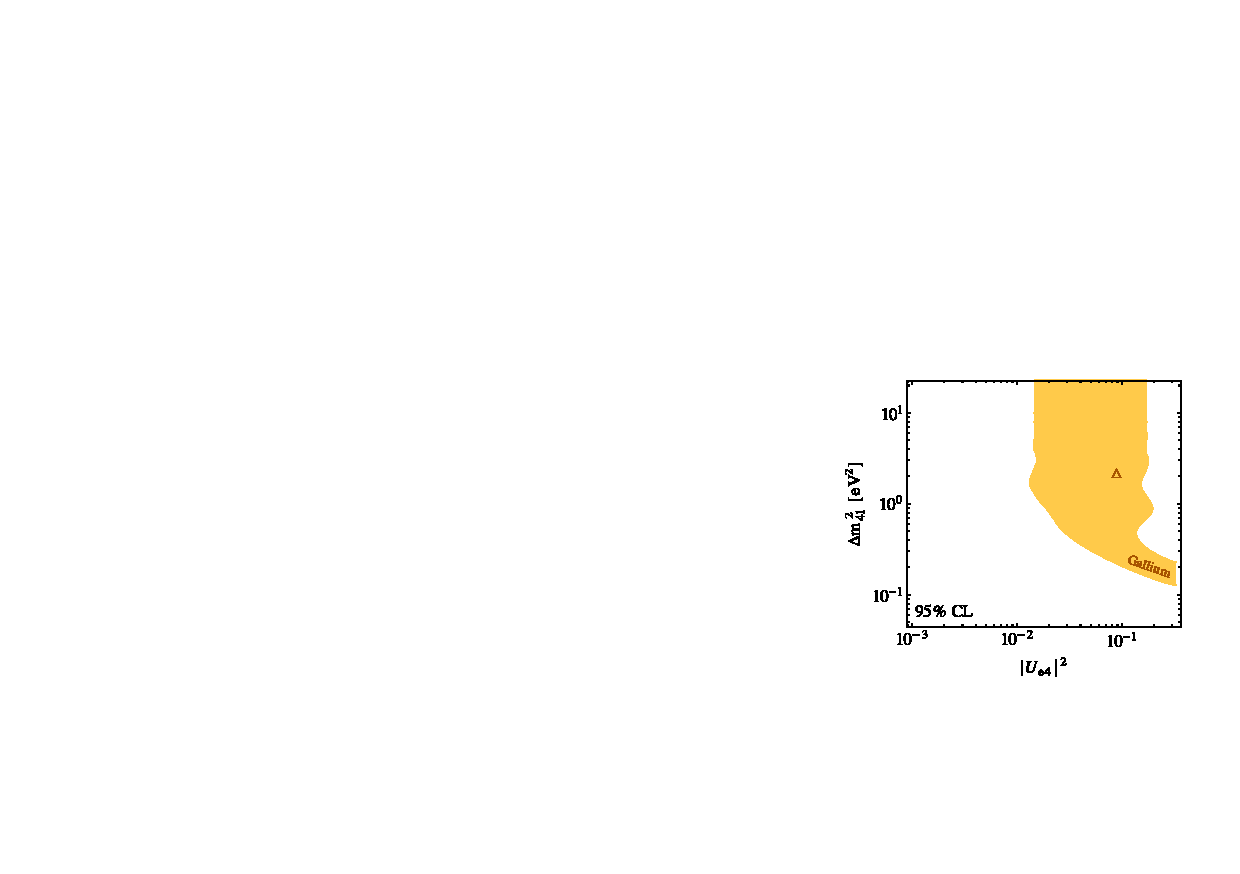
\includegraphics[width=\linewidth]{figures/radiochemical_space.pdf}
    \caption{Allowed parameter space for sterile neutrino oscillation.}
    \end{center}
  \end{subfigure}
  \caption{The SAGE and GALLEX experiments observed a deficit of electron neutrino interactions using radioactive isotopes, which could be explained by introducing oscillations into a sterile neutrino state.}\label{fig:radiochemical}
\end{figure}

Figure \ref{fig:radiochemical} shows the deficit for the four calibration runs (two with $^{51}$Cr for GALLEX, one with $^{51}$Cr and one with $^{37}$Ar for SAGE) and the allowed parameter space in the case of sterile neutrino oscillations in the 3+1 model.

Curiously, during the second data-taking run of SAGE, 2 tons of gallium were stolen from the detector (3.6\% of the total mass) \cite{Abdurashitov:1999zd}.
    
\subsection{Reactor experiments} 
Several reactor neutrino experiments have measured a deficit of events in the antineutrino spectra. This anomaly first appeared in 2011, when an improved calculation of the reactor antineutrino spectra was made available \cite{Mueller:2011nm}. Historical data from several reactor experiments, which before the recalculation were in agreement with the theoretical predictions, all showed a $\sim6\%$ deficit in the spectra, as shown in Figure \ref{fig:reactor}. 
    
    \begin{figure}[htbp]
      \centering
      \captionsetup{margin=1.3cm}
      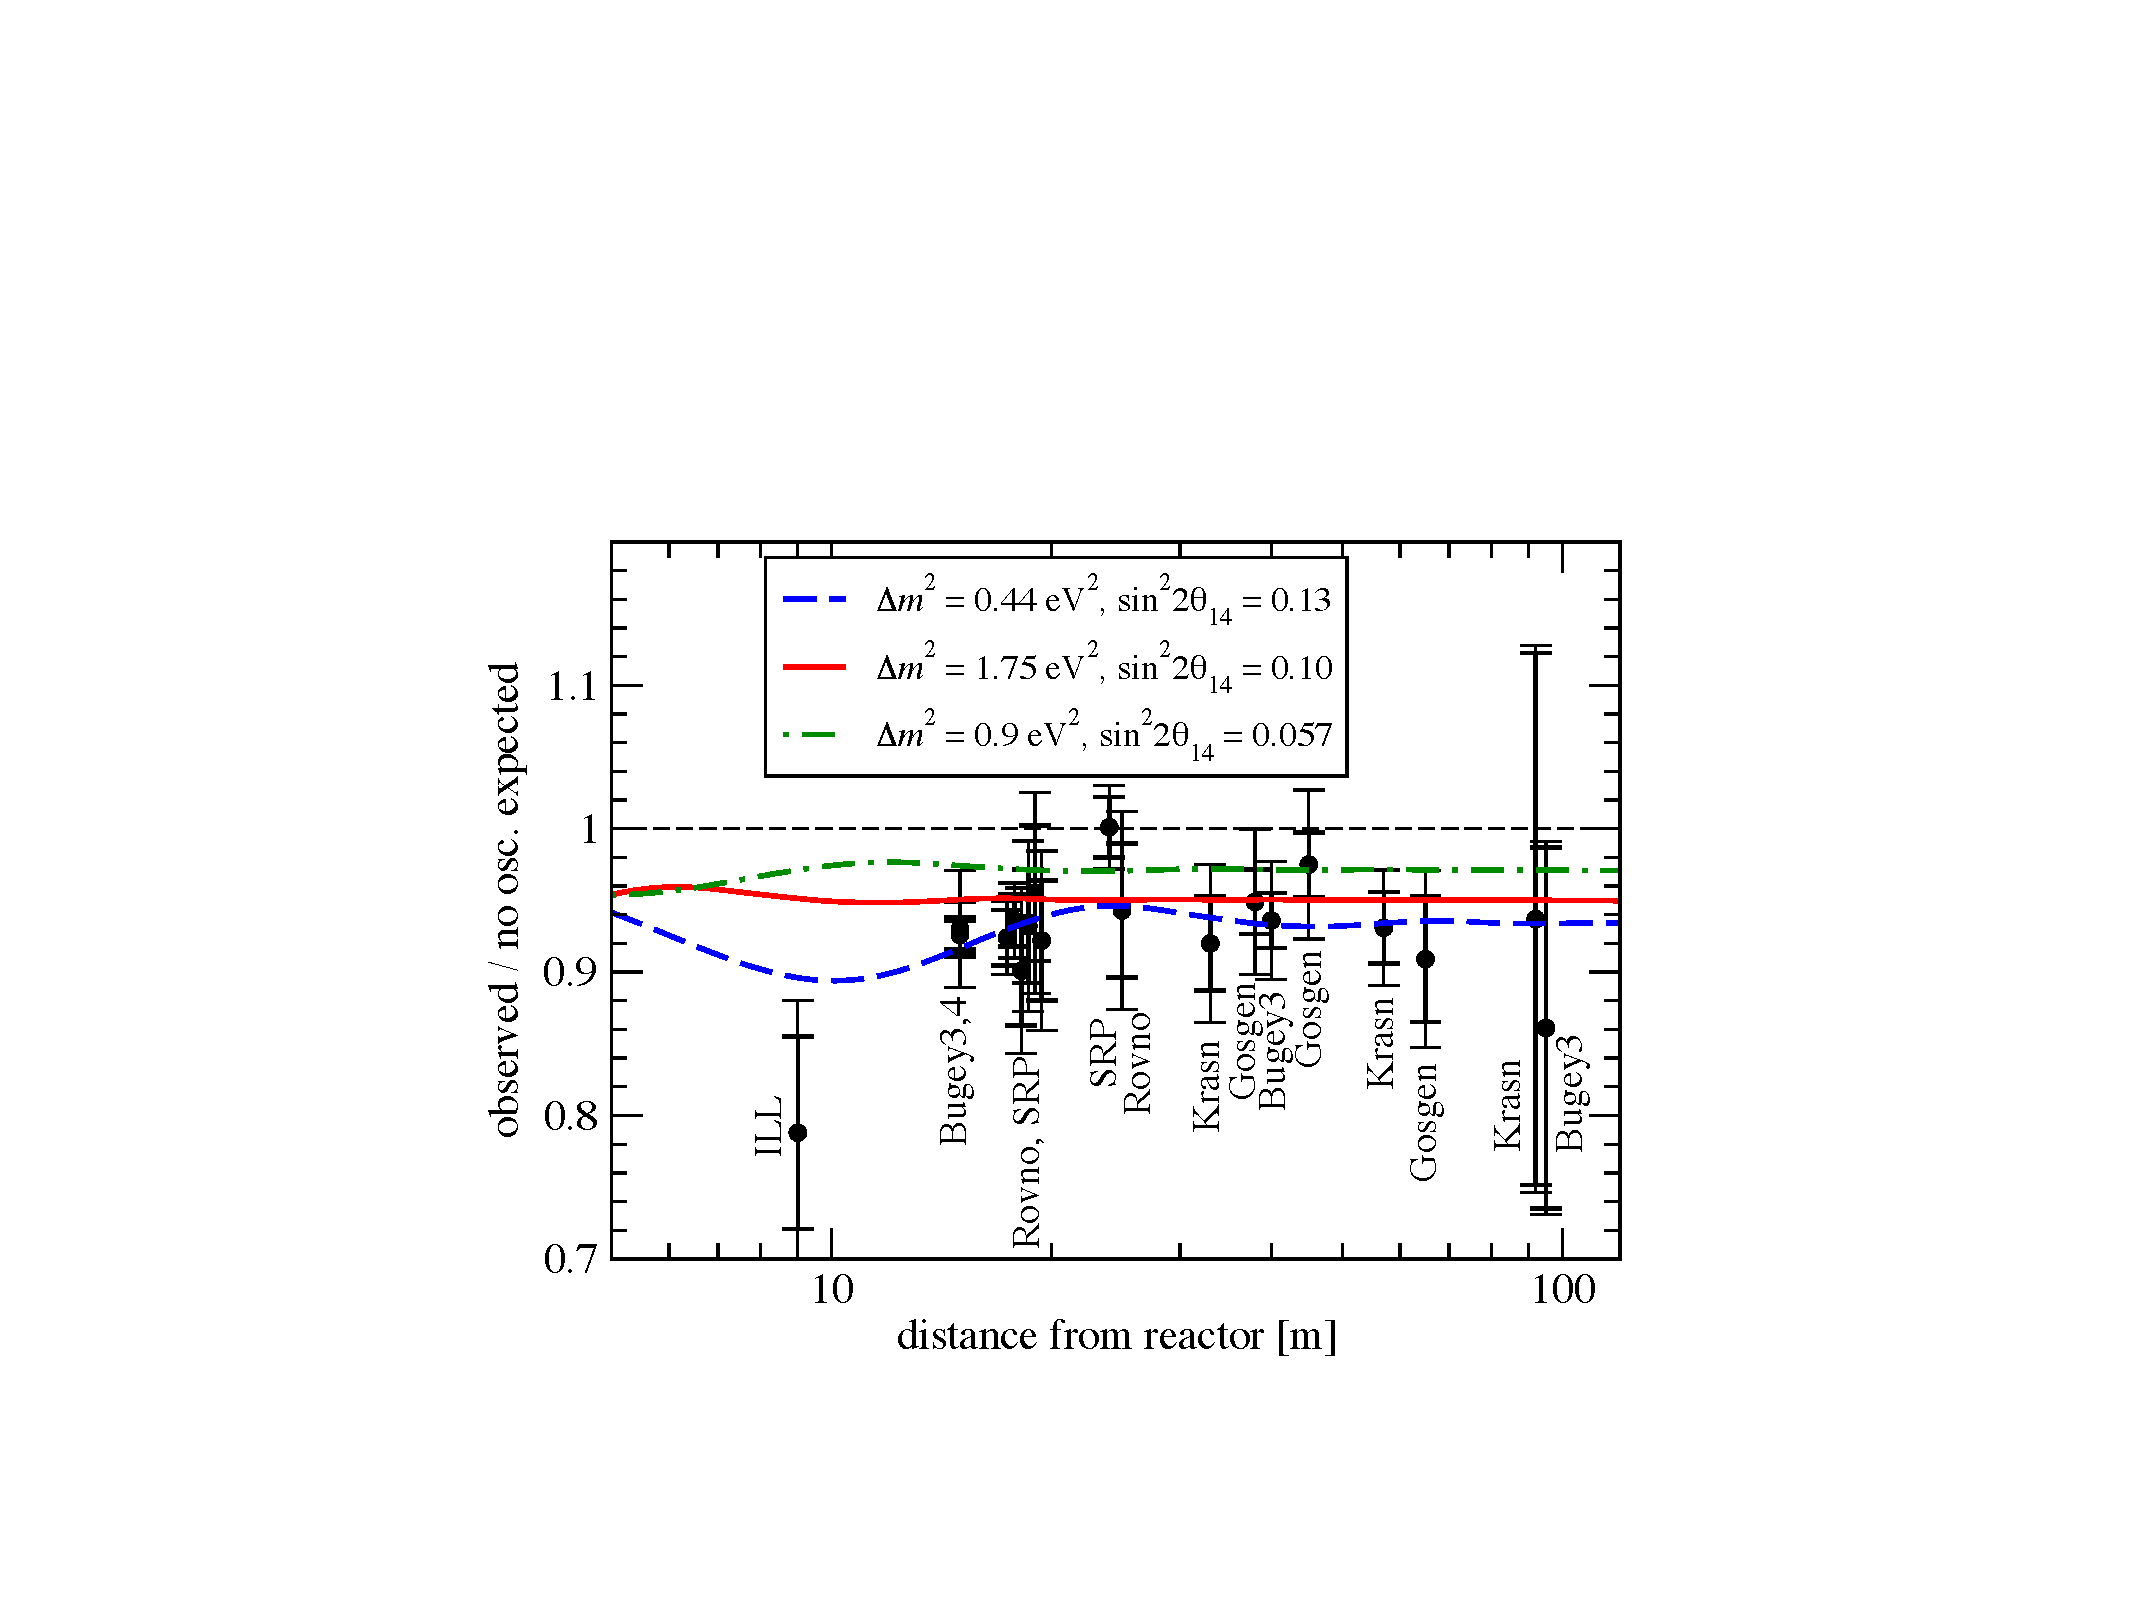
\includegraphics[width=0.75\linewidth]{figures/reactor.pdf}
      \caption{Fraction between observed and predicted $\bar{\nu}_{e}$ flux at several reactor neutrino experiments. Several models for sterile neutrino oscillation for different mass splitting terms and mixing angles are also shown.}
    \label{fig:reactor}
    \end{figure}
    
    This anomaly was first confirmed by a blind analysis of the Daya Bay collaboration \cite{An:2015nua} and then observed also by the RENO and Double Chooz detectors. More recently, these three experiments have also observed an excess of events (\emph{bump}) around 5~MeV. 
    In order to clarify the nature of the flux deficit, the Daya Bay experiment was able to correlate the antineutrino flux with the fuel composition in the reactor. The fuel evolves with time: the main fissile component, $^{235}$U, gets smaller, while the $^{239}$Pu increases. The model used to predict the inverse beta-decay yield is 3.1$\sigma$ in disagreement with data \cite{An:2017osx}. If the deficit is caused by sterile neutrinos, then it should not depend on the fissile material and the sterile neutrino hypothesis cannot be used to explain the fuel evolution model discrepancy. A combined analysis of Daya Bay and NEOS data hints to an excess production of $^{235}$U as an explanation for the 5~MeV bump \cite{Huber:2016xis}. 
    
    \begin{figure}[htbp]
      \centering
      \captionsetup{margin=1.3cm}
      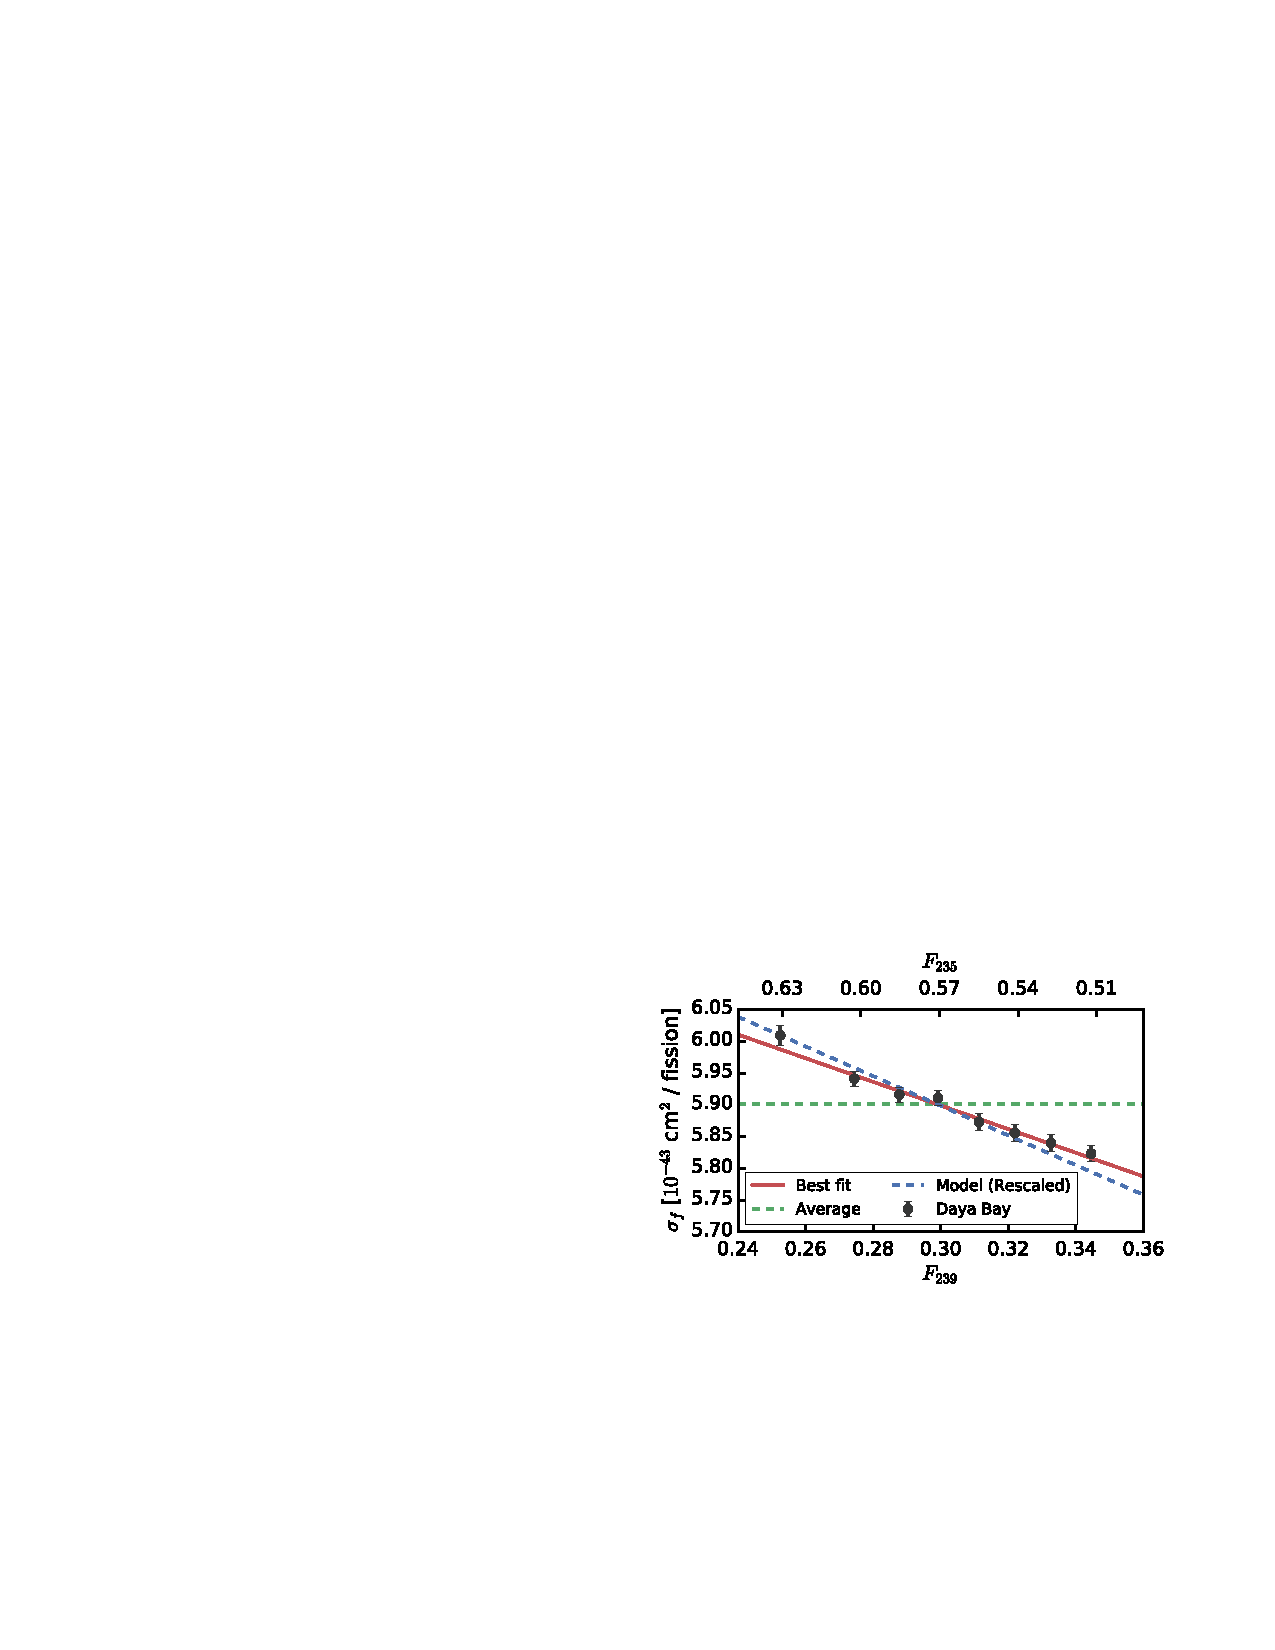
\includegraphics[width=0.75\linewidth]{figures/dayabay.pdf}
      \caption{Inverse $\beta$-decay yield per fission, $\sigma_f$, versus effective $^{239}$Pu (lower axis) or $^{235}$U (upper axis) fission fraction. Adapted from \cite{An:2017osx}.}
    \label{fig:dayabay}
    \end{figure}
    
    A new generation of reactor neutrino experiments should definitely solve the reactor anomaly. In particular, experiments like PROSPECT \cite{Ashenfelter:2015uxt} and SoLi$\partial$ \cite{Abreu:2017bpe}, will be placed very close to small fission cores and they will be sensitive to eventual short-baseline sterile neutrino oscillations.

\section{Constraints on the $(3+1)$ model}

In the presence of a sterile neutrino, its mixing with the active flavours would affect the $\nu_e$ appearance, the $\nu_e$ disappearance, and the $\nu_{\mu}$ disappearance probabilities. However, the combined analysis of MINOS, Daya Bay, and Bugey-3 $\nu_{\mu}$ disappearance data \cite{Adamson:2016jku} also excludes the best-fit point. A recent result from IceCube \cite{TheIceCube:2016oqi} further restricts the available parameter space, leaving little room for the $(3+1)$ hypothesis. 
The tension emerges both by comparing appearance and disappearance experiment (Figure \ref{fig:disapp}) and by comparing $\nu_e$ data ($\nu_e\rightarrow\nu_e$, $\nu_e\rightarrow\nu_{\mu}$) and $\nu_{\mu}$ data ($\nu_{\mu}\rightarrow\nu_{\mu}$) (Figure \ref{fig:nue_vs_numu}) in a global analysis \cite{Dentler:2018sju}.

\begin{figure}[htbp]
  \begin{subfigure}{0.48\textwidth}
    \begin{center}
    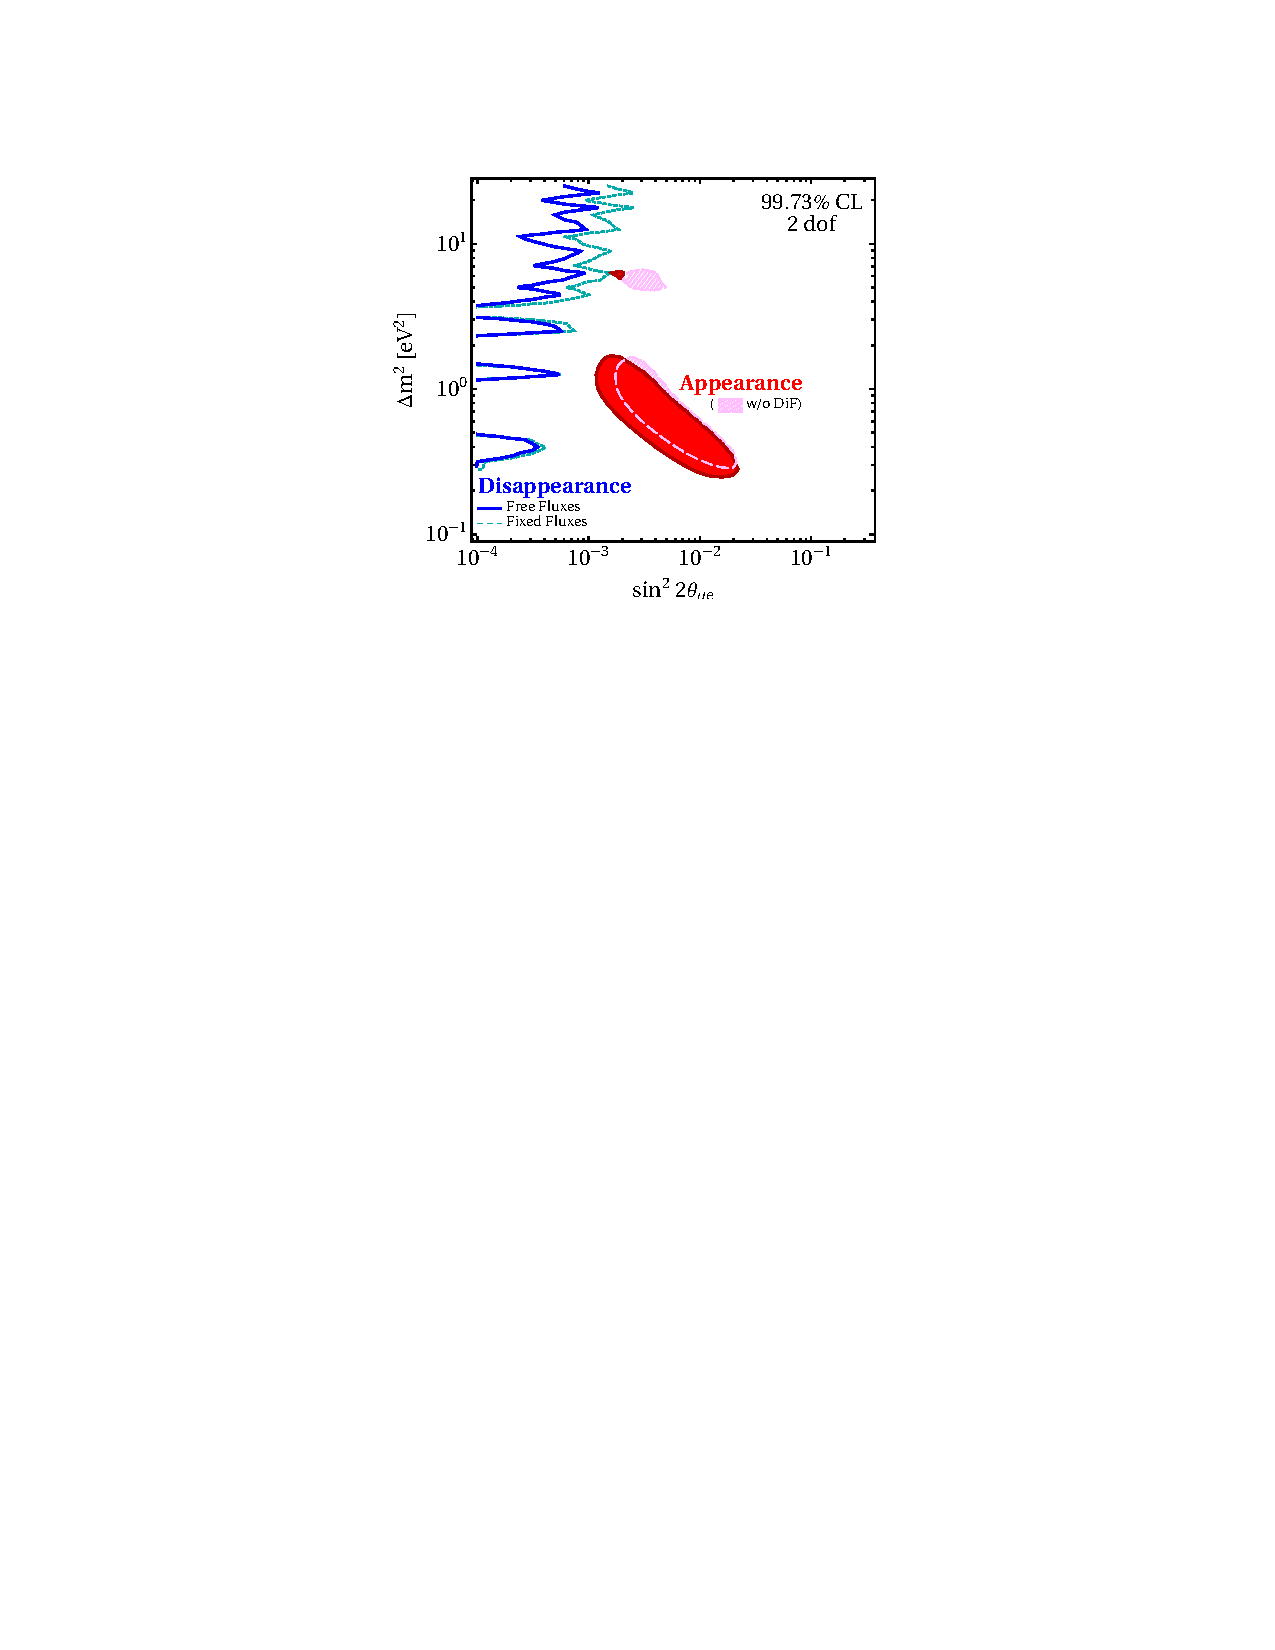
\includegraphics[width=\linewidth]{figures/disapp.pdf}
    \caption{Comparison between regions allowed by appearance results (filled red region) and regions excluded by disappearance results (solid blue line).}\label{fig:disapp}
    \end{center}
  \end{subfigure}\hfill
  \begin{subfigure}{0.48\textwidth}
    \begin{center}
    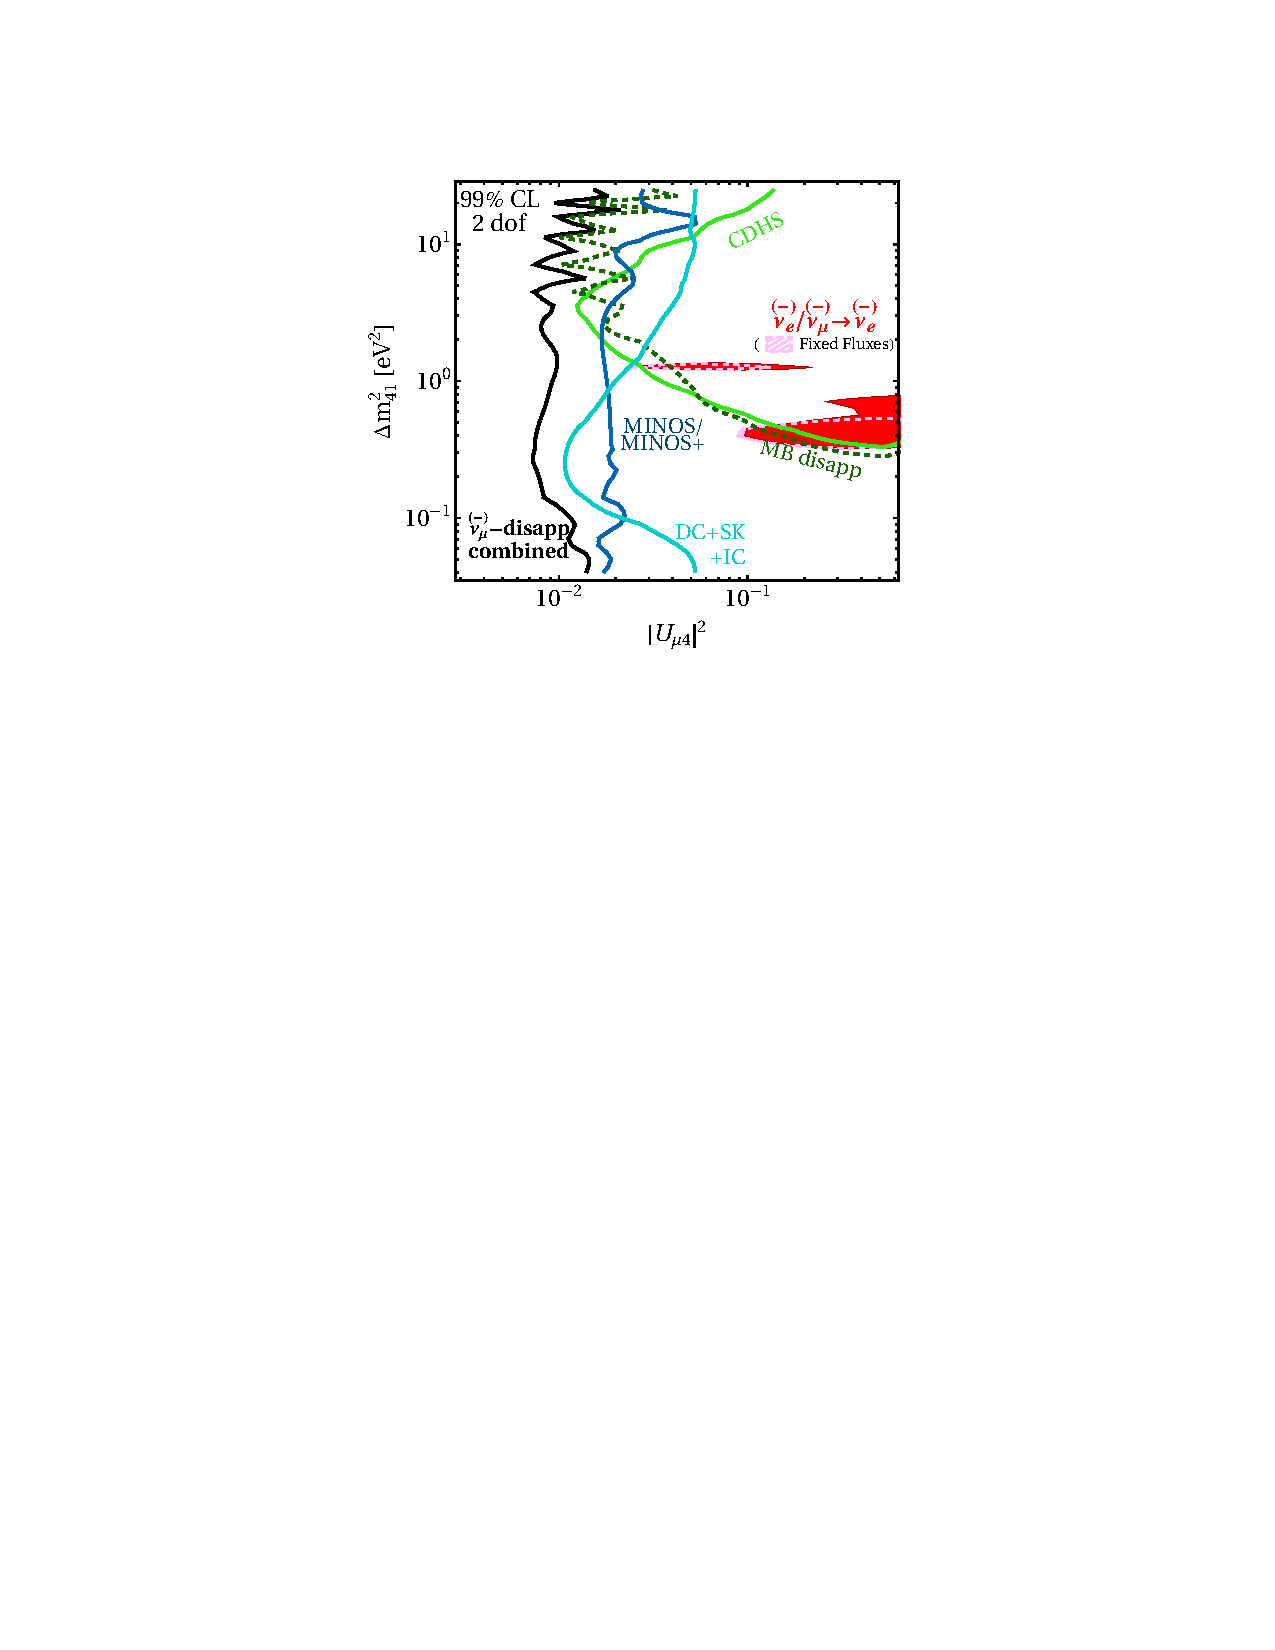
\includegraphics[width=\linewidth]{figures/nuenumu.pdf}
    \caption{Comparison between regions allowed by $\nu_e$ data ($\nu_e\rightarrow\nu_e$ and $\nu_e\rightarrow\nu_{\mu}$, filled red region) and regions excluded by $\nu_{\mu}$ disappearance data (solid lines).}\label{fig:nue_vs_numu}
    \end{center}
  \end{subfigure}
  \caption{There is a severe tension between appearance and disappearance results within the $(3+1)$ model. The free (fixed) fluxes lines of the plots on the left refer to the constraining (or not) of the reactor fluxes in the fits. Adapted from \cite{Dentler:2018sju}.}
\end{figure}


A proposed solution to these tensions is to introduce more than one sterile neutrinos. As such, other explanations have been proposed for the excess: $3+N$ sterile neutrinos with $N>1$ \cite{Conrad:2012qt}, CPT violation \cite{Kostelecky:2011gq}, and resonant neutrino oscillations \cite{Asaadi:2017bhx} among the others. The explanation of the excess with the presence of a new particle decaying or scattering in the detector is severely constrained by kinematic arguments \cite{Jordan:2018qiy}.

After the definitive confirmation of neutrino oscillations, achieved by employing different detection techniques, a series of new experiments collected data not fully compatible with a three-flavour scenario. In particular, a combined analysis of the LSND and MiniBooNE data gives a $6.0\sigma$ significance for an excess of electron neutrinos. This result is however in tension with other experiments if interpreted as the oscillation into a sterile neutrino state. 

Other experiments have also performed measurements not fully in agreement with the theoretical expectations, using both reactor antineutrinos and neutrinos from radioactive isotopes, but a coherent explanation for these anomalies still has to be provided. 
\chapter{\label{ch:4-microboone}The MicroBooNE experiment}

\minitoc


This chapter presents an overview of the MicroBooNE experiment, with a focus on the Liquid Argon Time Projection Chamber technology. A description of the MicroBooNE detector is essential in order to understand the analysis described in the following chapters. The selection efficiency of low-energy electron neutrino events and the rejection of background events can directly depend on the detector properties. The analysis is also affected by systematic uncertainties in the detector simulation, which will be partially addressed here. A brief description of the MicroBooNE neutrino beam will also be provided.

\section{Motivation}
The MicroBooNE (Micro Booster Neutrino Experiment) experiment is an 89~t active volume Liquid Argon Time Projection Chamber (LArTPC) located at the Fermi National Accelerator Laboratory (FNAL) in Batavia, IL and on-axis with the Booster Neutrino Beam (BNB). The experiment was designed to study short-baseline neutrino oscillations and neutrino-argon cross section. It is the largest neutrino LArTPC detector currently active in the world.
This technology offers very high spatial resolution and calorimetric capabilities, which allow for detailed tracking, vertexing, and particle identification. 

\subsection{Physics goals}
As described in Section \ref{sec:miniboone}, MiniBooNE, being a Cherenkov detector, is not able to distinguish between single photons and electrons in the final state. As such, it is not possible to determine the nature of the excess of low-energy events. If the excess is caused by photons, one explanation could be provided by an underestimation of one of the background components. An electron nature of the excess, instead, could be a strong hint for BSM physics.

\subsubsection{Addressing the MiniBooNE anomaly}
The MicroBooNE experiment was designed to definitely clarify the MiniBooNE anomaly since the LArTPC technology allows for powerful electron/photon separation. One way to achieve this goal is to measure the spatial gap between the neutrino interaction vertex and the start of the electromagnetic shower. An electron will start producing a ionising trail immediately, whereas a photon will usually leave a visible gap, due to the radiation length in liquid argon $X_0 = 14$~cm.
A second way to distinguish between electrons and photons is to measure the energy loss per distance travelled ($dE/dx$) of the electromagnetic shower produced in the liquid argon. For electrons above 100~MeV, the theoretical expectation of the most probable $dE/dx$ is around 2~MeV/cm, while the photon will have a most probable value approximately twice as large, due to the pair-production process $\gamma\rightarrow e^+e^-$ \cite{Acciarri:2016sli}. 
\mccorrect{In order to clarify MiniBooNE result}, MicroBooNE is then performing two parallel analyses, one assuming that the excess is caused by photon production in the electromagnetic $\Delta\rightarrow N\gamma$ decay and one assuming that the excess is caused by electron interactions. \mccorrect{In this way, we will be able to definitely identify the nature of the excess and check if it is caused by electron neutrino interactions or by an underestimation of one of the backgrounds.} The calorimetric and spatial-resolution capabilities will allow having a sensitivity to the excess similar to MiniBooNE, while having an active detector mass five times smaller.  The search for electron-like low-energy interactions will be described in detail in the following chapters.

\subsubsection{Cross-section measurements}
MicroBooNE will also provide precise neutrino-nucleon cross-section measurements. The neutrino interactions in the energy range of the BNB span from quasi-elastic to deep inelastic scattering, making it possible to explore several nuclear effects and complex topologies.
In particular, it is possible to measure the pion production in neutral current (NC) and charged current (CC) interactions. MicroBooNE should be able to solve the tension between the large NC $\pi^0$ component reported by MiniBooNE \cite{AguilarArevalo:2008xs} and the small CC $\pi^+$ component reported by SciBooNE \cite{Hiraide:2008eu} and K2K \cite{Tanaka:2006zm}. 
A precise measurement of the photon production will also help to constrain the $\Delta\rightarrow N\gamma$ background, important for the MiniBooNE low-energy excess analysis. 

The measurement of neutrino cross sections in liquid argon is also of fundamental importance for the design of the largest next-generation neutrino experiment, DUNE (Deep Underground Neutrino Experiment). Its current proposed design includes a 40-kton LArTPC as far detector, two orders of magnitude larger than MicroBooNE \cite{Acciarri:2016ooe}.

\subsubsection{Supernova and exotic searches}
The MicroBooNE detector is located just below the surface level and is constantly bombarded by cosmic rays, which interact in the liquid argon leaving ionisation trails. This background, together with the small active volume of the detector (compared with large-scale water Cherenkov experiments) can limit the capabilities of certain physics analyses, such as proton decay searches. However, MicroBooNE can study the interaction of charged kaons in the liquid argon, which can represent a background to future proton decay searches in DUNE.
The existence of proton decay is predicted by several Grand Unification Theories (GUTs) and a lower proton lifetime of $5.9\times10^{33}$ years was set by the Super-Kamiokande experiment looking at the $p\rightarrow \nu K^+$ channel \cite{Abe:2014mwa}. The kaon decay chain $K\rightarrow\pi\rightarrow\mu\rightarrow e$ represents also an important benchmark for the reconstruction capabilities of the LArTPC.

The MicroBooNE detector is suited to detect neutrinos produced by a supernova (SN) in the Milky Way or in its immediate surroundings, which would result in around 30 CC $\nu_e$ interactions with electron energy above 10~MeV. However, being constantly hit by cosmic rays, the detector cannot directly trigger on SN neutrinos and it relies on the SuperNova Early Warning System (SNEWS) \cite{Antonioli:2004zb} to record an eventual SN event. 


\subsection{Research and development goals}
MicroBooNE is currently the largest active neutrino LArTPC in the world, which makes it the first experiment to precisely assess the automated neutrino reconstruction capabilities of this technology. The detection of neutrinos by a large-scale LArTPC was pioneered by the ICARUS collaboration, which designed and assembled the ICARUS T600 detector \cite{Amerio:2004ze}. The detector consists of two LArTPC modules with a total active mass of 476~t, around five times larger than MicroBooNE. However, it was employed as a long-baseline neutrino detector on the CNGS (CERN Neutrinos to Gran Sasso) beam and it detected only four $\nu_e$ interactions \cite{Antonello:2013gut}, compared with the several hundred expected at MicroBooNE. It was recently refurbished and moved to Fermilab to be placed on the BNB, as a part of the future Short Baseline Neutrino (SBN) program. On a smaller scale, the ArgoNeuT experiment operated a 0.25~t TPC on the NuMI neutrino beam at Fermilab \cite{Anderson:2012vc} and measured for the first time the neutrino cross section on argon atoms.

The ambitious physics program of the DUNE experiment, whose ultimate goal is to verify the presence of CP violation in the leptonic sector, requires a very good understanding of the technology: in particular, the effect of high electric field on long distances, of the ions recombination in the LAr, and of the ions absorption by the impurities must be precisely quantified. 
MicroBooNE was also the first large-scale LArTPC to have part of the electronics chain operating directly in the liquid argon (\emph{cold electronics}), allowing for higher signal-to-noise ratio. An overview of the MicroBooNE detector will be provided in Section \ref{sec:detector}.
A small-scale prototype of the DUNE detector, ProtoDUNE, was recently built and commissioned at CERN, with an active mass of 450~t. The ProtoDUNE detector, however, runs on a test-beam line and will not detect neutrino interactions.

\section{The LArTPC detection technology}
The concept of a Liquid Argon Time Projection Chamber was first laid out by Willis and Radeka in 1974 \cite{Willis:1974gi} and then adapted by Rubbia in 1977 as a detector for neutrino interactions \cite{Rubbia:1977zz}. 

Generally speaking, a Time Projection Chamber is a volume with a constant electric field applied between two of its sides, the anode (the positive plane) and the cathode (the negative plane). It is possible to fill the volume with a non-conductive material such as inert gases or liquids. %A magnetic field can also be applied to measure the charge and the momentum of the particle interacting in the TPC (it is not the case of MicroBooNE). 

A charged particle traversing the medium inside the TPC will ionise the material: a trail of ionisation electrons will be produced in correspondence with the path of the charged particle. The constant electric field will transport the electrons towards the anode with a constant drift velocity, preserving their topological and calorimetric information and appearing as a projection of the particle trajectory on the anode plane. The distance between the anode and the interaction point will be given by the time the ionisation electron takes to reach the anode. Figure \ref{fig:lartpc_diagram} shows the operating principle of a TPC in the case of the MicroBooNE detector. 

\begin{figure}[htbp]
    \centering
    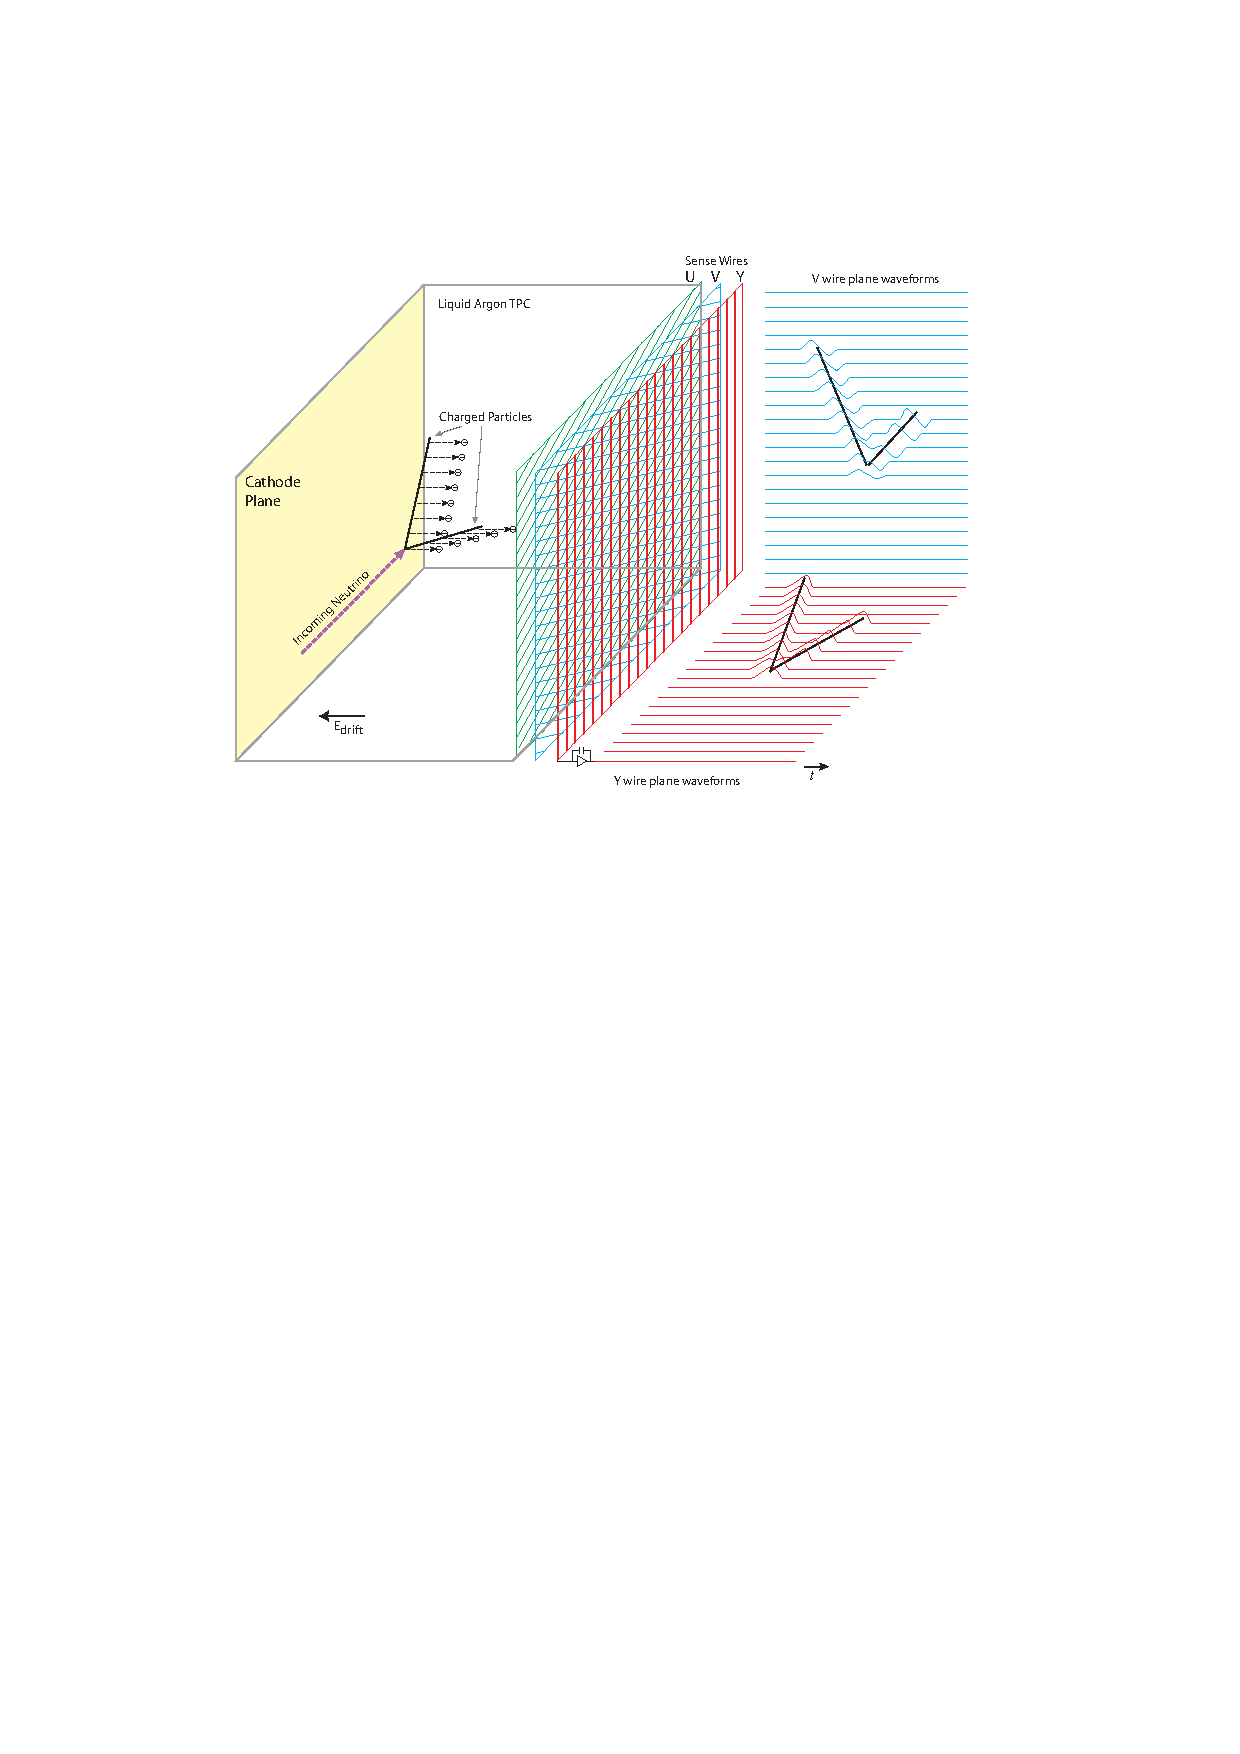
\includegraphics[width=0.8\linewidth]{figures/lartpc_diagram.pdf}
    \caption{Diagram of the operating principle of the MicroBooNE LArTPC, showing the waveforms produced by the ionisation trails in the collection plane (red) and in one induction plane (blue).}
    \label{fig:lartpc_diagram}
\end{figure}

As the name says, a LArTPC is a TPC filled with liquid argon. This material provides several advantages, which made this technology particularly suitable for neutrino detection. Among the main ones we can enumerate (1) its substantial density (1.4~g/cm$^3$ at 87.3~K), which allows to have a detectable amount of neutrino interactions, (2) its high stability, being a noble gas, and (3) its natural abundance (1\% of the atmosphere), which makes the LArTPC technology highly scalable and affordable.

However, the relatively slow drift velocity of the electrons in the liquid argon causes the typical read-out of a large-scale LArTPC to be in the order of the milliseconds (which corresponds to the time a ionisation electron takes to travel from the cathode to the anode), making this technology sub-optimal for high-rate experiments. 

Another fundamental property of the argon, which makes it particularly suitable for high-energy physics experiments, is that it produces scintillation light when excited, being at the same time transparent to the wavelength of this scintillation light, described below. In this way, a detector on surface such as MicroBooNE can collect the light (in our case with photomultipliers placed inside the LAr) and trigger the TPC readout in coincidence with the neutrino beam, suppressing the background caused by cosmic rays outside the beam time window. 

A LArTPC can achieve a very high spatial resolution, similar to the one of the bubble chambers, allowing at the same time for the digitisation of the signal. For this reason, it has often been called a \emph{fully electronic bubble chamber} \cite{Rubbia:2011zza}. 

\subsubsection{Light production}
The scintillation light is produced when an atom of argon in the ground state shares an electron with one argon of atom in an excited state, forming an Ar$_{2}$ \emph{excimer}. When the excimer decays and a 128~nm photon is emitted, the two argon atoms are both left in the ground state. This small wavelength is typically difficult to detect with standard photomultipliers. In the MicroBooNE experiment, the PMT plates are coated with tetraphenyl butadiene (TPB), which acts as wavelength shifter. The time distribution of the scintillation light emission has two characteristics components at 6~ns and 1.5 \si{\micro}s.

The liquid argon has also a high light yield, comparable to the one of scintillating crystals, with $4\times10^4$~$\gamma$/MeV. The amount of light, however, can be quenched by the presence of nitrogen impurities in the argon, which, in the case of MicroBooNE, are kept below the 2~ppm level.

\subsubsection{Ionisation electrons}\label{sec:ionisation}
The work function for ionising an argon atom is $W_{\mathrm{ion}} = 23.6$~eV, which means that a charged particle in the MeV range will leave a ionisation trail of tens of thousands of electrons. Under an electric field, these free electrons will travel towards the anode with a constant drift velocity, but during their path they can undergo several attenuation processes, which decrease the actual number of electrons reaching the wire plane. 

In particular, the electrons can recombine with ionised Ar$^+$ atoms: this recombination effect is usually the main contributor to the signal attenuation. This effect depends on the $dE/dx$ of the particle, on the electric field in the liquid argon, and on the angle of the ionisation particle with respect to the electric field. The ICARUS experiment measured the dependence of the recombination as a function of the $dE/dx$ and the applied electric field \cite{Amoruso:2004dy}, as shown in Figure \ref{fig:recombination}. The ArgoNeuT experiment found the recombination effect in a LArTPC to be well described both by the Birks' model \cite{Birks:1951boa} and by a modified version of the Box model \cite{Thomas:1987zz}. 

\begin{figure}[htbp]
\centering
  \begin{subfigure}{0.48\textwidth}
    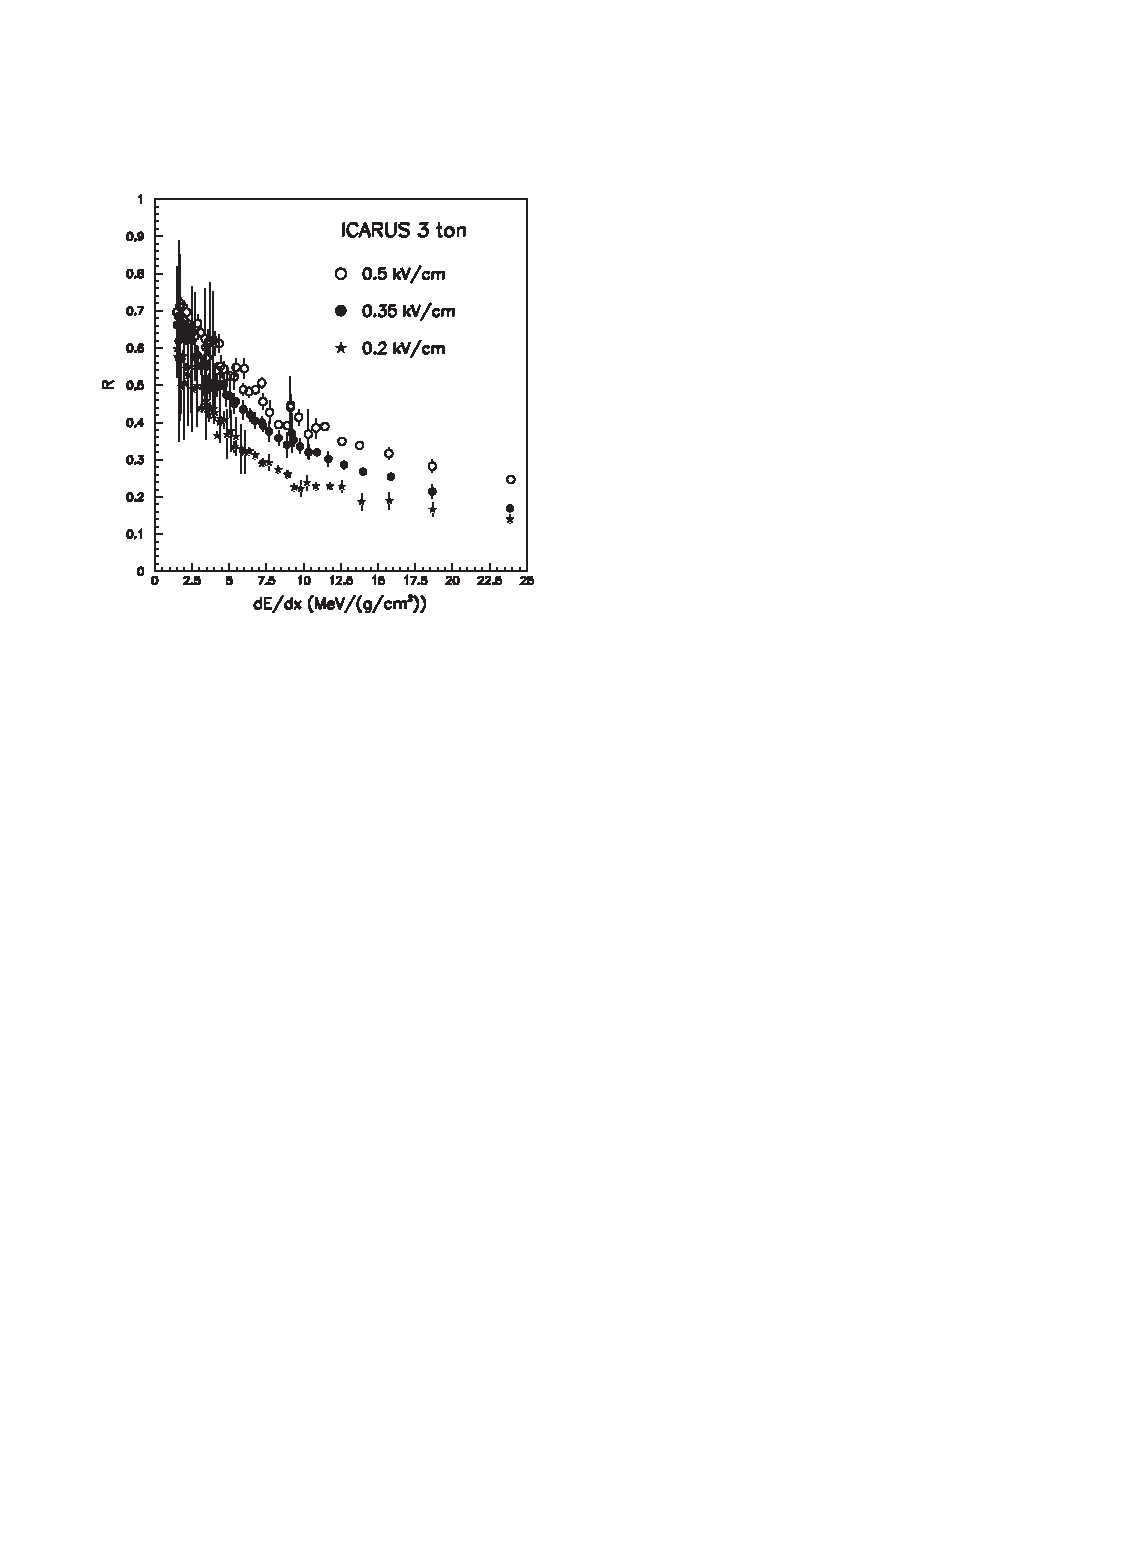
\includegraphics[height=0.9\linewidth]{figures/icarus1.pdf}
    \caption{Recombination factor as a function of the particle $dE/dx$.}
  \end{subfigure}\hfill
  \begin{subfigure}{0.48\textwidth}
    \begin{center}
        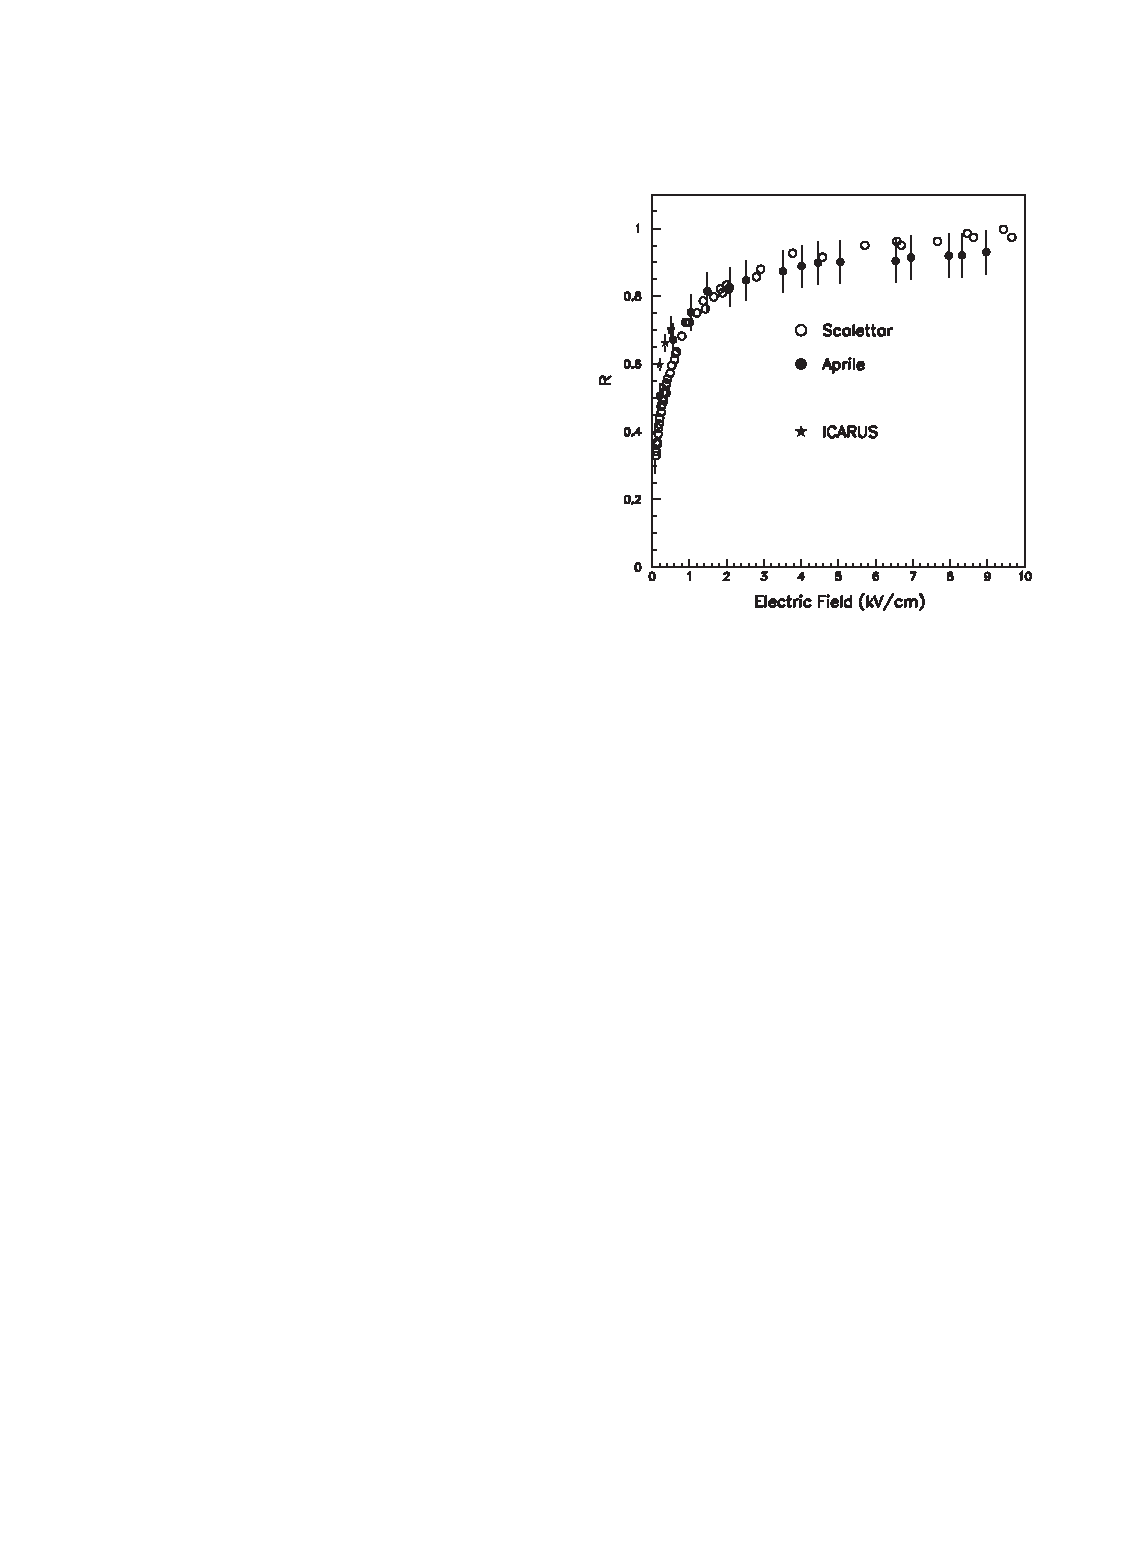
\includegraphics[height=0.9\linewidth]{figures/icarus2.pdf}
        \caption{Recombination factor as a function of the electric field in the detector.}
    \end{center}
  \end{subfigure}
    \caption{The ICARUS collaboration measured the recombination factor \emph{R}, defined as the ratio between the measured and the theoretical stopping power, as a function of the $dE/dx$ (left) and of the electric field (right). From \cite{Amoruso:2004dy}.}\label{fig:recombination}
\end{figure}

The transport of the electrons in the LArTPC is affected by diffusion, caused by their thermal velocity, which spreads out the ionisation electrons while they travel towards the anode. It is a three-dimensional effect, usually separated into its longitudinal and transverse components. 

LArTPCs placed on surface, such as MicroBooNE, are also constantly hit by an intense flux of cosmic rays, which will produce several ionisation trails. These trails produce ionisation electrons and positive Ar$^+$, with the ions slowly moving towards the cathode until they will recombine with a free electron. The build-up of Ar$^+$ ions leads to a distortion of the electric
field within the detector, defined as \emph{space-charge effect} (SCE). The SCE causes a displacement in the reconstructed position of ionisation electrons, as well as variations in the amount of charge quenching experienced by ionisation throughout the volume of the TPC. In MicroBooNE, the electric field distortion can be as high as 15\% and was measured using a sample of cosmic rays triggered by a small cosmic-ray counter (briefly described in Section \ref{sec:crt}) \cite{sce}. The spatial distortions at the top and the bottom of the LArTPC are shown in Figure \ref{fig:spacecharge}.

\begin{figure}[htbp]
    \centering
    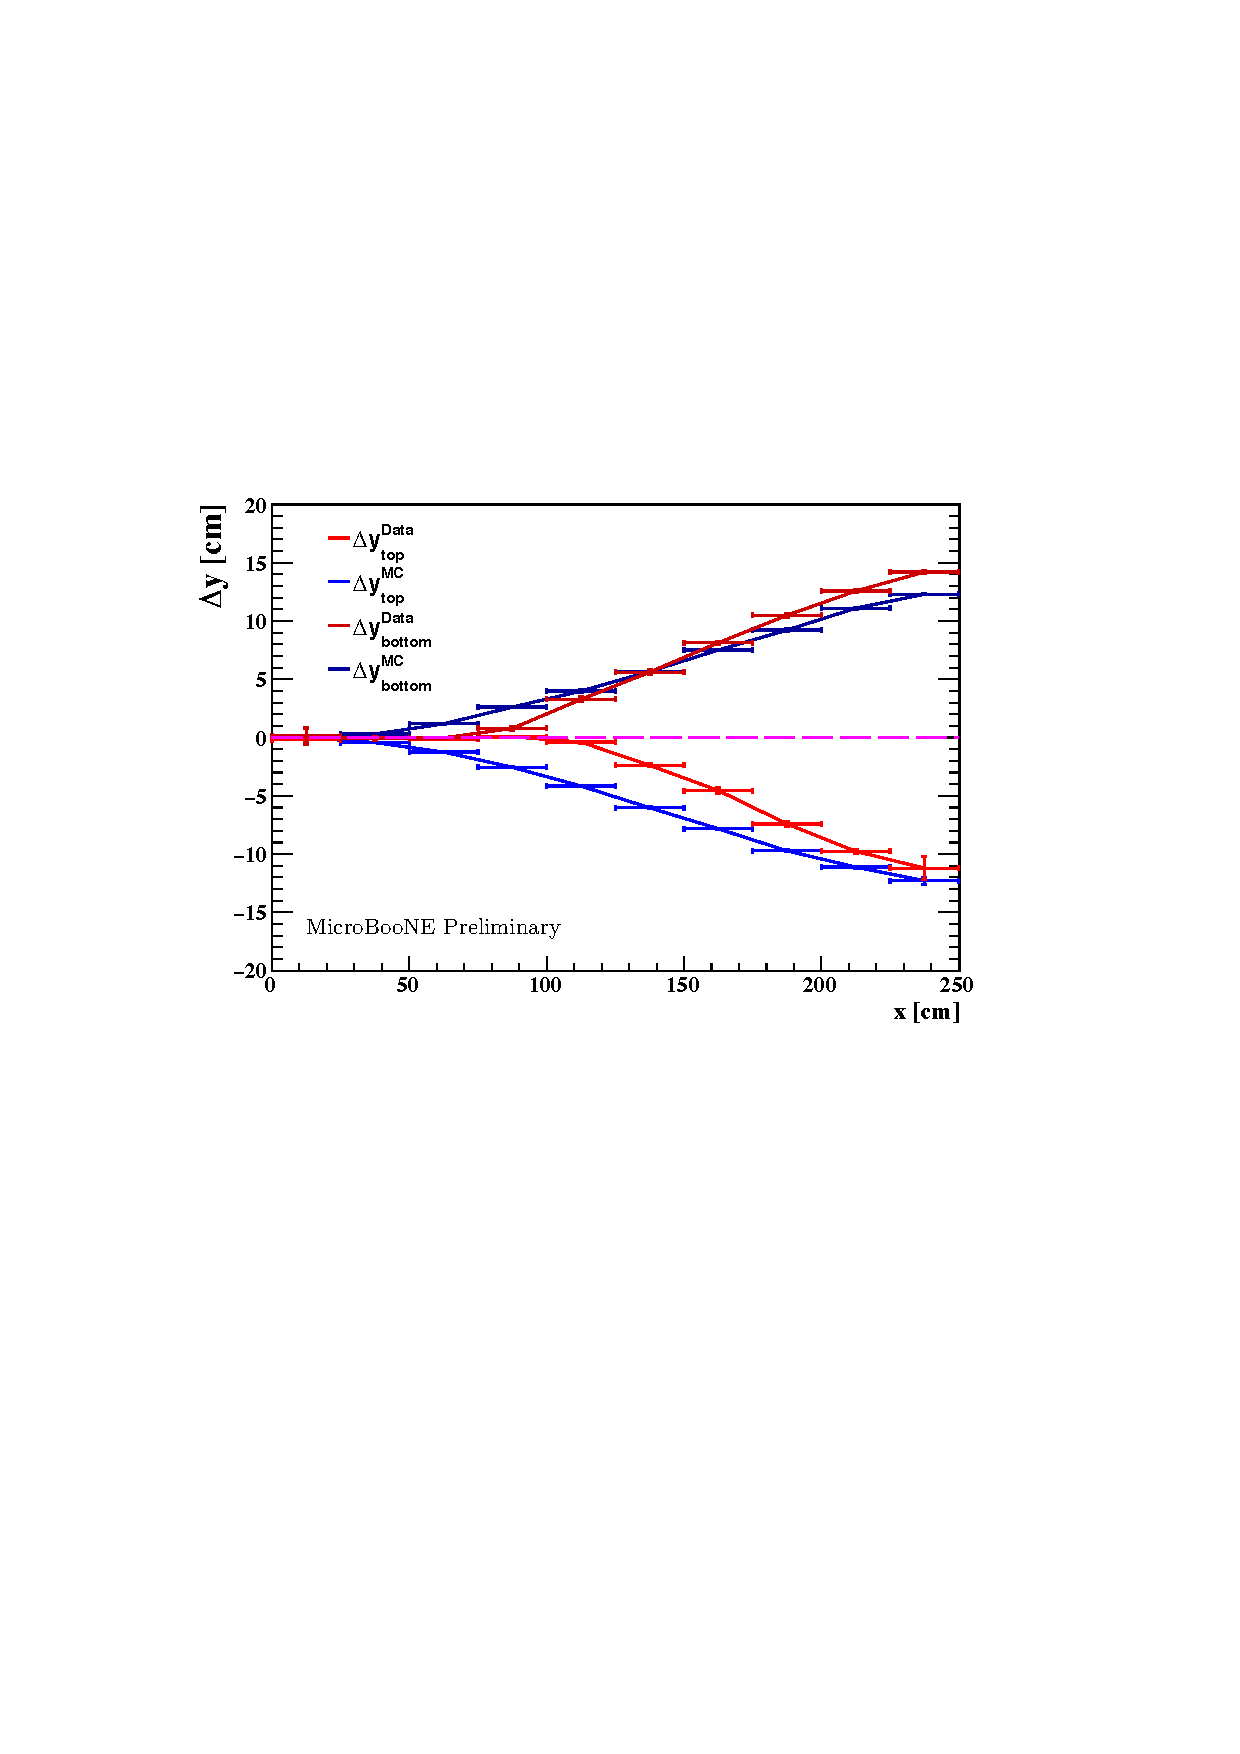
\includegraphics[width=0.8\linewidth]{figures/spacecharge.pdf}
    \caption{Predicted ($\Delta y^{\mathrm{MC}}$) and measured ($\Delta y^{\mathrm{Data}}$) space-charge distortions as a function of the drift coordinate at both the top and bottom of the TPC. The discrepancy between data and Monte Carlo is caused by the absence of the liquid argon flow in the simulation. Error bars are statistical only. From \cite{sce}.}
    \label{fig:spacecharge}
\end{figure}

The presence of impurities in the liquid argon, such as oxygen, nitrogen, and water can also attenuate the signal, absorbing the ionisation electrons during their path in the liquid argon. The amount of drifting electrons decline as a function of the distance from the wire plane, since the electrons need to travel a longer path. The attenuation is well modelled by an inverse exponential function and the decay time constant is called \emph{electron lifetime}. MicroBooNE purification system, described in Section \ref{sec:detector}, achieved an O$_2$ contamination smaller than 100~ppt and an electron lifetime larger than 18~ms \cite{Meddage:2017lxo}. In MicroBooNE, the electron lifetime was estimated by measuring the ratio between the charge at the anode and the charge at the cathode with crossing cosmic muons, through the relation:
\begin{equation}
    \frac{Q_A}{Q_C} = \exp(-t_{\mathrm{drift}}/\tau),
\end{equation}
where $t_\mathrm{drift}$ is the drift time (2.3~ms) and $\tau$ is the electron lifetime. Figure \ref{fig:purity} shows the variation of the $Q_A/Q_C$ ratio over time in the MicroBooNE LArTPC.

\begin{figure}[htbp]
    \centering
    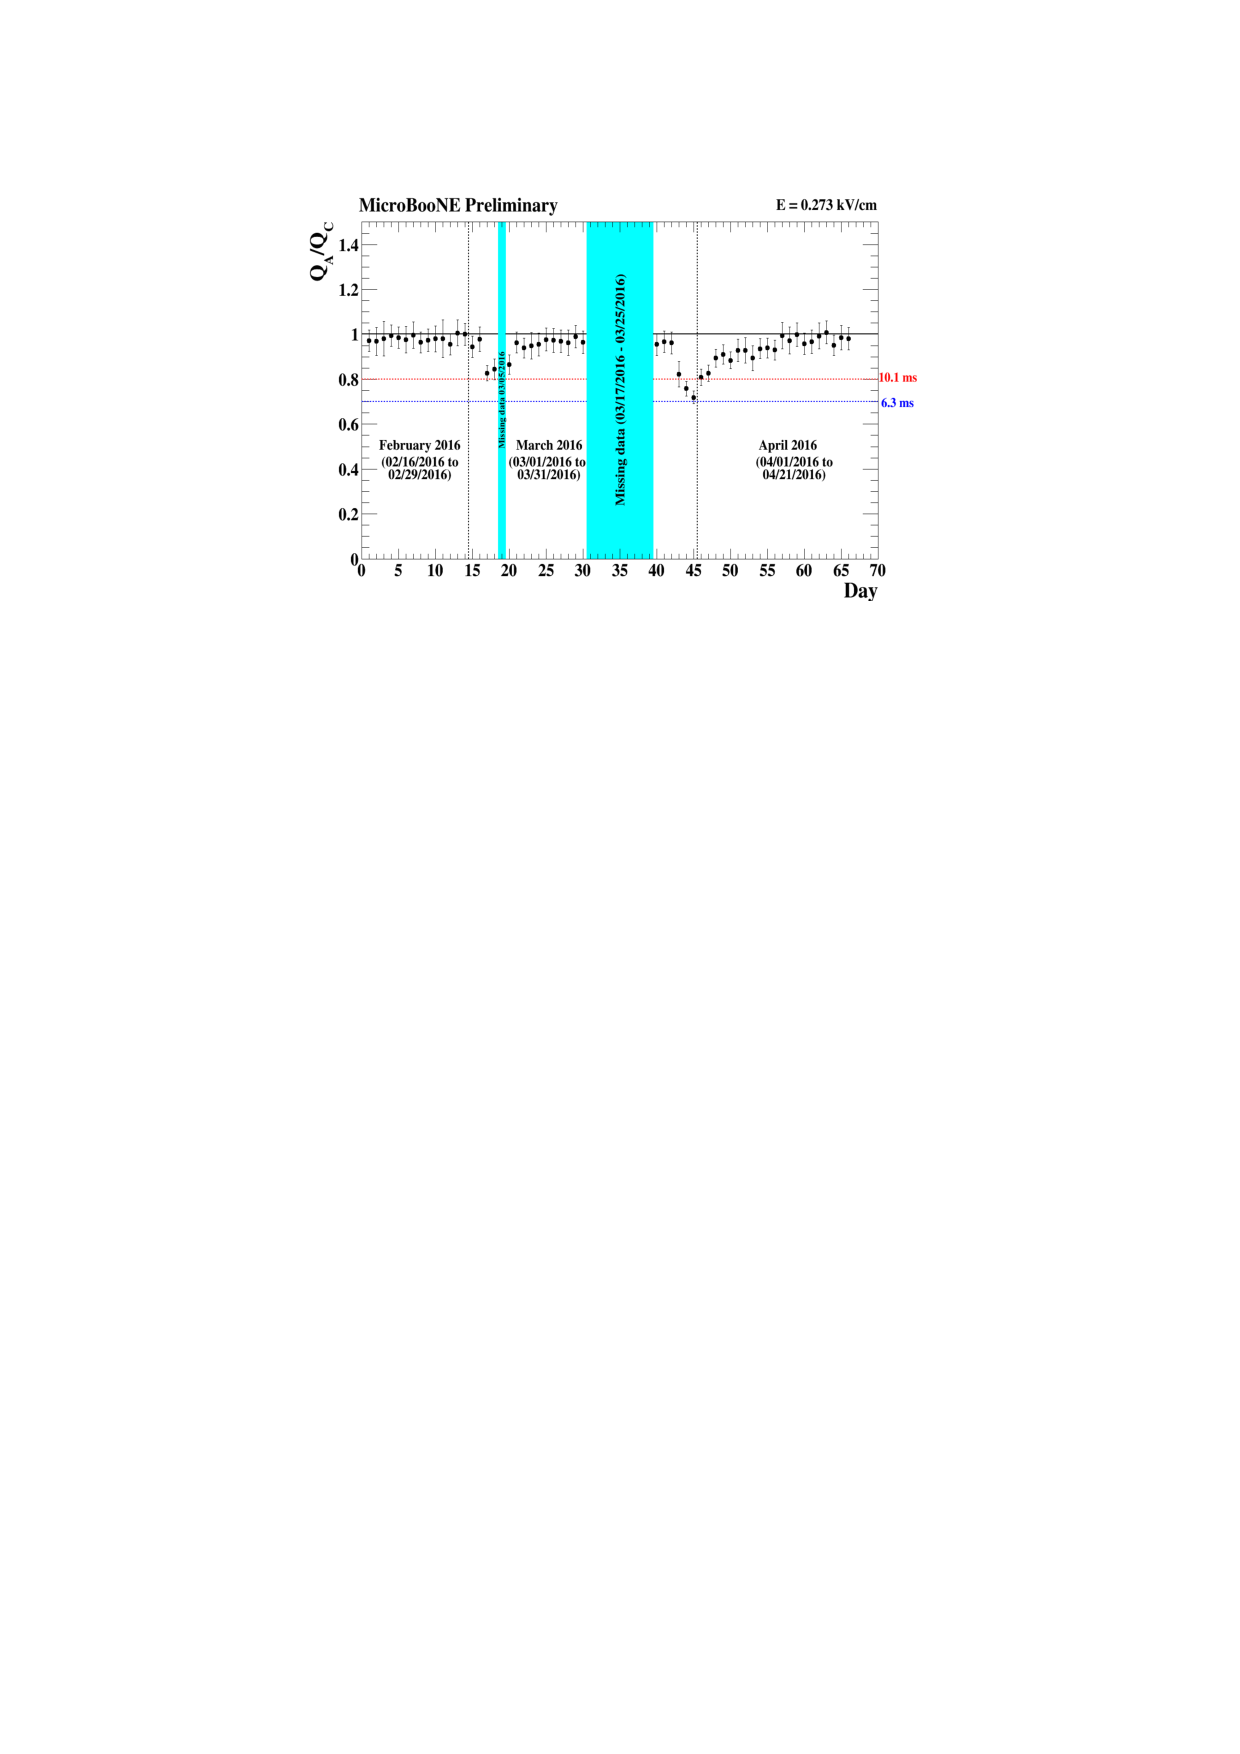
\includegraphics[width=0.7\linewidth]{figures/purity.pdf}
    \caption{Variation of the $Q_A/Q_C$ charge ratio between February and April 2016 in the MicroBooNE LArTPC. From \cite{Meddage:2017lxo}.}
    \label{fig:purity}
\end{figure}
 
\section{The neutrino beams at Fermilab}\label{sec:beam}
The use of an artificial neutrino source presents two main advantages: (1) the neutrino energy spectrum and its flavour components can be precisely characterised and tuned for the specific physics goals, and (2) the position of the detector can be optimised to observe the oscillation peak (or dip). The design of a neutrino beam generally follows the same pattern: it starts with a proton beam, which hits a target and produces hadrons. These hadrons are focused by a magnetic horn into an empty pipe, where they decay, producing the neutrinos. The neutrino beam then travels through the ground and hits one or more neutrino detectors.

At Fermilab, there are two neutrino beams currently active: the Booster Neutrino Beam (BNB) and the Neutrinos from the Main Injector (NuMI) beam, with different energy, flavour composition, and direction. MicroBooNE is placed on-axis with the BNB and 470~m far from the target. While it is also able to detect off-axis neutrinos from the NuMI beam, the analysis presented in this document will focus on the neutrinos coming from the BNB.

The accelerator chain starts with a source of hydrogen gas, which is ionised and accelerated by an empty cavity with -35~kV voltage. This H$^-$ stream is focused by two solenoids and transformed into a pulsed beam 100~\si{\micro}s long at 15~Hz. The Radio Frequency Quadrupole (RFQ) then accelerates the beam to an energy of 750~keV. The H$^-$ beam is then fed to the Linear Accelerator (LINAC), where two series of RF cavities bring it from 750 keV to 400~MeV.  The negative hydrogen ions are stripped of their electrons by a carbon foil and the proton beam is finally injected into the Booster synchrotron. Here, after several thousand laps, the proton beam reaches their maximum kinetic energy in the Booster of 8~GeV.

The 8~GeV proton batch is 1.6~\si{\micro\second} long and divided into 84 bunches 2~ns wide. From the Booster, the proton batch can be extracted to the Booster Neutrino target or be injected into the Main Injector, where it is accelerated up to 120~GeV.

\subsection{The Booster Neutrino Beam}
The BNB is the main neutrino beam for the MiniBooNE and MicroBooNE experiments and it will be used also for the future Short Baseline Neutrino program \cite{Antonello:2015lea}. It was designed mainly for the MiniBooNE experiment and, in order to suppress the background coming from resonant and DIS interactions (as described in Section \ref{sec:modes}), its neutrino flux is peaked below 1~GeV.

The BNB target is made of a beryllium disk 0.51~cm in radius and 71.1~cm long, which corresponds to 1.7 interaction lengths. This material minimises the radiative losses due to its relatively low density. The number of protons hitting the target (protons-on-target, POT) is measured by two toroids placed upstream the target within a 2\% uncertainty. Each BNB bunch usually delivers $4\times10^{12}$ POT. 

\begin{figure}[htbp]
    \centering
    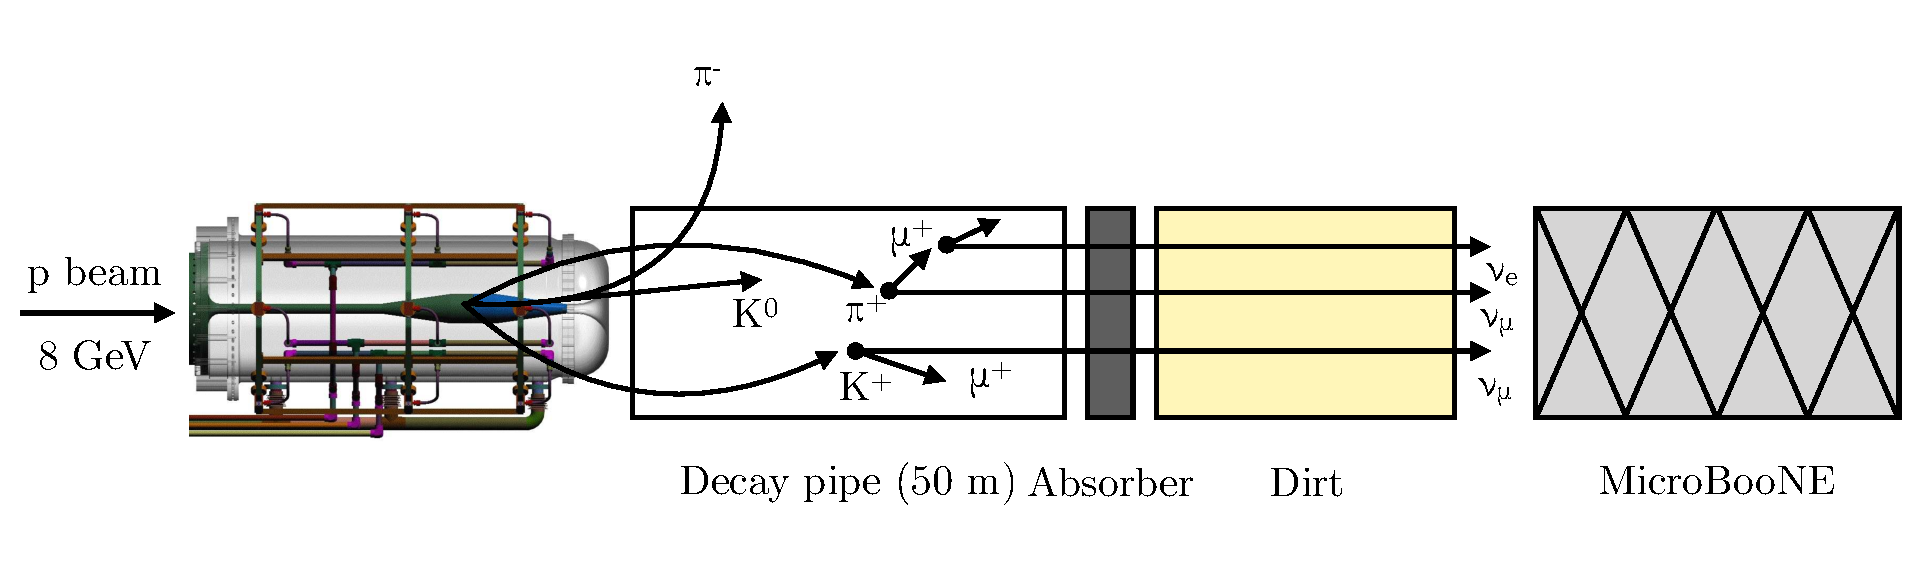
\includegraphics[width=0.98\linewidth]{figures/neutrinobeam.pdf}
    \caption{Schematic of the Booster Neutrino Beam chain in neutrino mode, showing, from left to right, the focusing horn, the decay pipe, the absorber, and the dirt. Dimensions are not to scale.}
    \label{fig:neutrinobeam}
\end{figure}

The hadrons produced in the p-Be interactions are then focused by the electromagnetic horn. The horn is a pulsed toroidal electromagnet with a peak current of 170~kA and a magnetic field at the centre of 1.5~T. It focuses the secondary hadrons along the horn axis: depending on the direction of the current, the positive (negative) charged particles are focused (deflected), producing a neutrino (antineutrino) beam. 

The hadrons with the right charge, mainly kaons and pions, travel through the decay pipe filled with air and are then stopped by a concrete absorber. The neutrinos produced in the decays travel through the ground and hit the detector, which in the case of MicroBooNE is placed 470~m far from the target. Figure \ref{fig:neutrinobeam} shows a schematic of the Booster Neutrino Beam stages in the neutrino mode. 

The muon neutrinos come from the decay of the pions (and in turns of the muons) and the decay of the kaons. Muons and kaons are also responsible for the electron neutrino contamination in the beam. Figure \ref{fig:bnbflux} shows the flavour composition of the BNB flux in neutrino mode at the MicroBooNE location.

\begin{figure}[htbp]
    \centering
    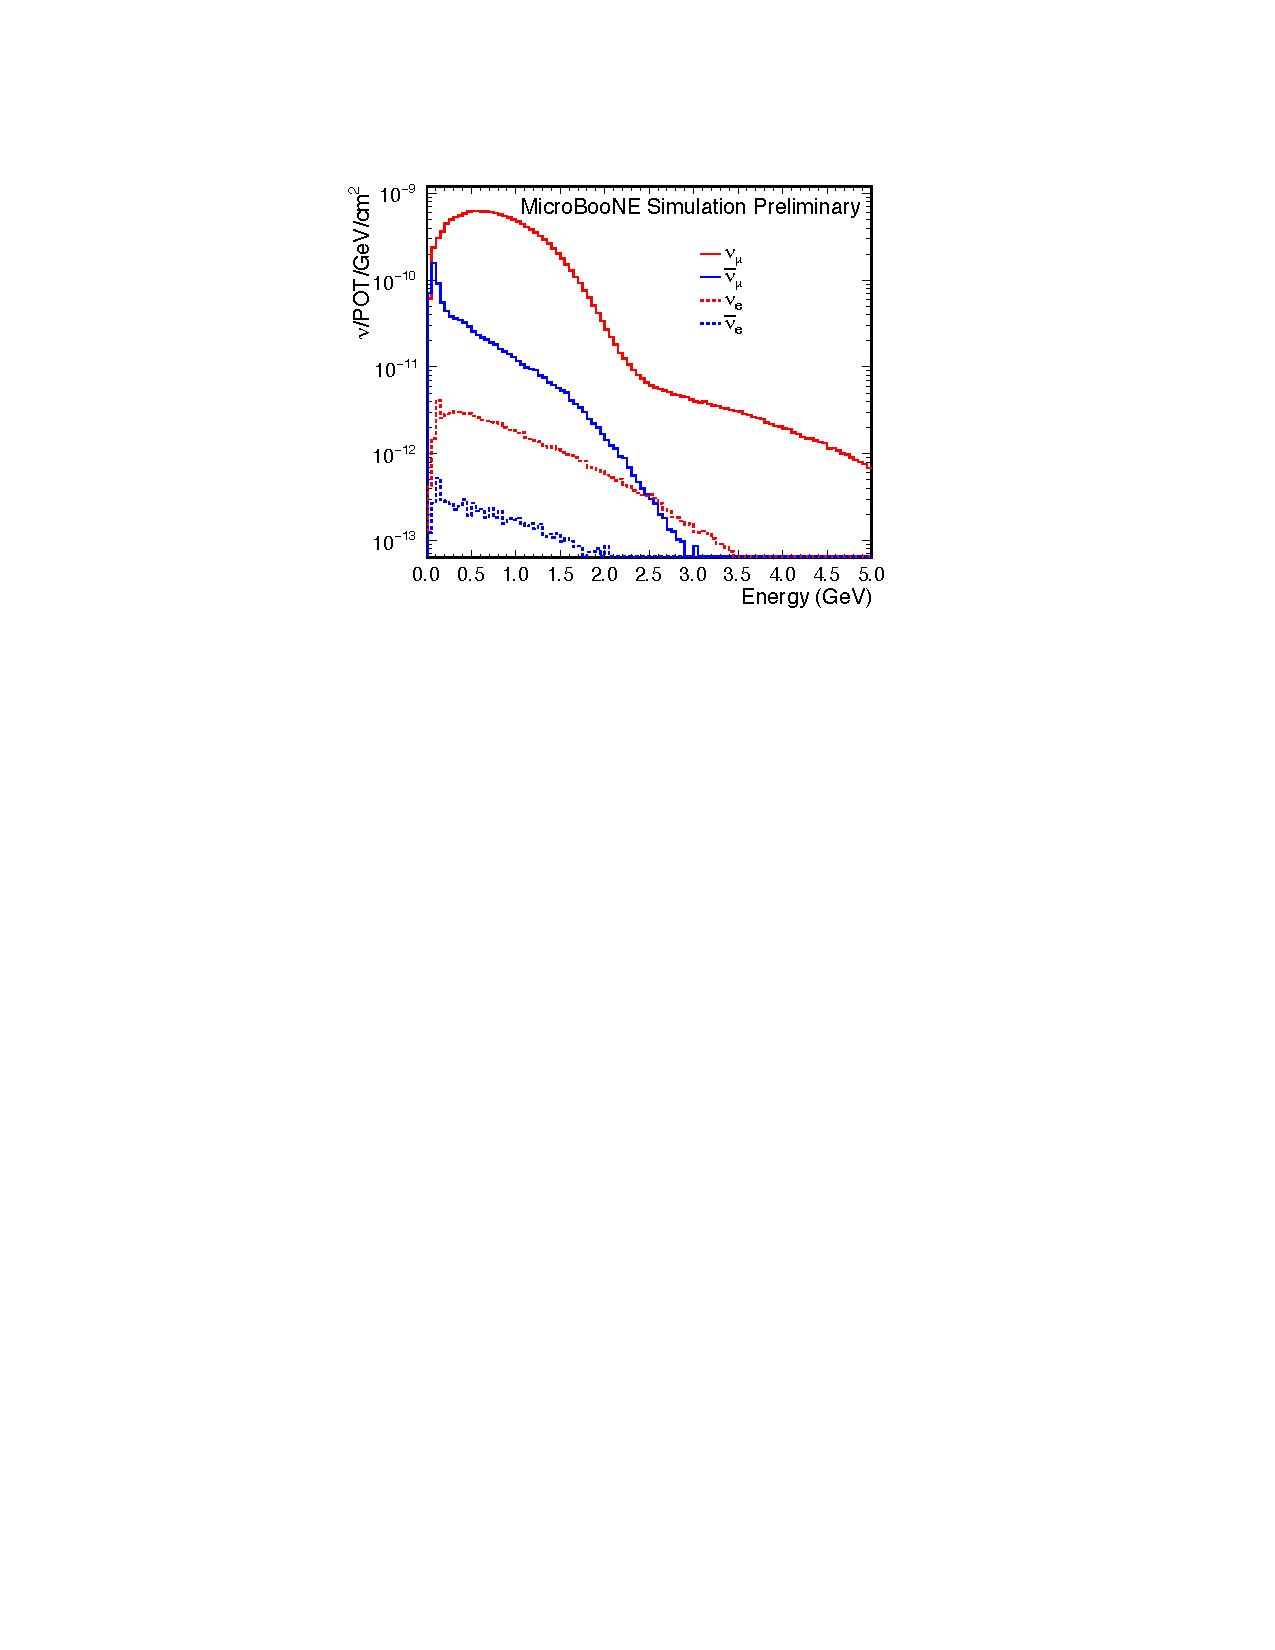
\includegraphics[width=0.7\linewidth]{figures/bnbflux.pdf}
    \caption{BNB absolute flux prediction in neutrino mode at the MicroBooNE location, break down by neutrino flavour.}
    \label{fig:bnbflux}
\end{figure}


The pulsed structure of the neutrino beam is of fundamental importance for on-surface experiments like MiniBooNE and MicroBooNE. In order to suppress non-beam related backgrounds (such as cosmic rays), the detector is triggered only in coincidence with the beam-gate window. In this way, MiniBooNE achieved a cosmic-ray background rejection of 99.987\% \cite{AguilarArevalo:2008qa}. For a LArTPC such as MicroBooNE, the cosmic-ray rejection is more challenging, since the data acquisition window must be at least as long as the drift time window (so in the order of the milliseconds). The techniques employed to reject cosmic rays will be described in Section \ref{sec:methodology}.
 
\subsection{Neutrino flux simulation}\label{sec:flux}
The MiniBooNE collaboration developed a detailed simulation of the BNB flux, described in \cite{AguilarArevalo:2008yp}. 

Here, we will enumerate the main stages of the simulation, in order to clarify the flux systematic uncertainties assessment in Section \ref{sec:systematics}:
\begin{description}
\item[Beamline geometry.] The geometry of the beamline components is simulated in detail, including the beam horn, the target, and the decay pipe. 
\item[Proton generation.] The number of protons delivered by the beam must be precisely estimated, accounting also for beam optics effects.
\item[Interactions of protons with the target.] This is the step with the largest uncertainty. The MiniBooNE collaboration estimated the $\pi^+$ and $\pi^-$ production using the data from the HARP experiment \cite{Catanesi:2005rc}, while the $K^+$ component was constrained using the result of the SciBooNE experiment \cite{Cheng:2011wq}. 
\item[Propagation in the material.] The interaction of the particles in the material is simulated with the GEANT toolkit \cite{Brun:1994aa}.
\item[Particles decay into neutrinos.] The branching ratios and the kinematic properties of the particles which produce the neutrino beam must be assessed with precision.
\end{description}

Table \ref{tab:flux_syst} shows the uncertainties on the various components of the BNB flux for the MicroBooNE experiment. These uncertainties will be reflected in the flux systematic uncertainties of the analysis described in Section \ref{sec:systematics}.

\begin{table}[htbp]
   \centering
     \caption{Systematic uncertainties on the BNB flux calculation. The other category includes uncertainties in pion and nucleon cross-sections on beryllium and aluminium, as well as the horn current calibration uncertainty, and uncertainty in the horn current distribution.}
   \begin{tabular}{p{0.28\linewidth}p{0.1\linewidth}p{0.1\linewidth}p{0.1\linewidth}p{0.1\linewidth}}
     \toprule
     Systematic uncertainty & $\nu_{\mu}/\%$ & $\bar{\nu}_{\mu}/\%$ & $\nu_e/\%$ & $\bar{\nu}_e/\%$ \\
     \midrule
     Proton delivery & 2.0 & 2.0 & 2.0 & 2.0 \\
     $\pi^+$ & 11.7 & 1.0 & 10.7 & 0.03 \\ 
     $\pi^-$ & 0.0 & 11.6 & 0.0 & 3.0 \\
     $K^+$ & 0.2 & 0.1 & 2.0 & 0.1 \\
     $K^-$ & 0.0 & 0.4 & 0.0 & 3.0 \\
     $K^0_L$ & 0.0 & 0.3 & 2.3 & 21.4 \\
     Other & 3.9 & 6.6 & 3.2 & 5.3 \\
     \midrule
     Total & 12.5 & 13.5 & 11.7 & 22.6~\%\\
     \bottomrule
   \end{tabular}
\label{tab:flux_syst}
\end{table}


\section{The MicroBooNE detector}\label{sec:detector}
The MicroBooNE detector consists of a rectangular LArTPC with dimensions of $256~$cm (width) $\times~233~$cm (height) $\times~1037~$cm (length) placed in a cylindrical cryostat. It sits on-axis with the BNB, 470~m far from the neutrino beam target. The mass of liquid argon in the active volume, defined as the portion of the argon encompassed by the TPC, is 89~t. 

\begin{figure}[htbp]
    \centering
    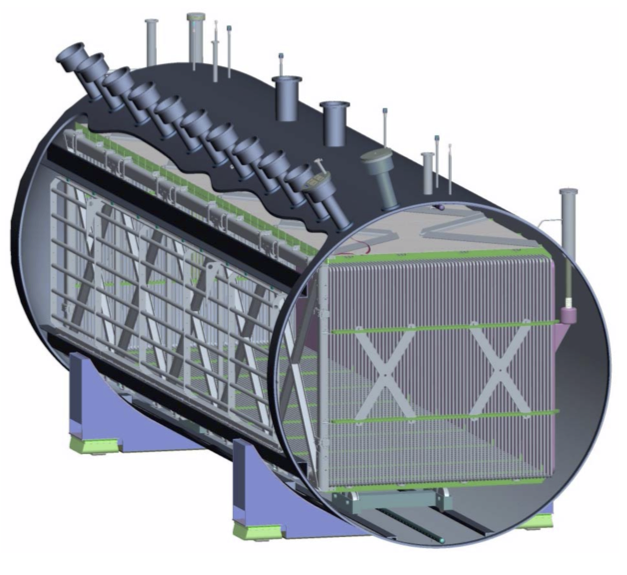
\includegraphics[width=0.7\linewidth]{figures/detector.png}
    \caption{3D rendering of the MicroBooNE cryostat, showing the TPC wire cage and the feedthroughs, which take the signals from the wires and the PMTs (not shown) to the DAQ. In this rendering, the cathode is on the right and the wire planes on the anode side are not shown.}
    \label{fig:detector}
\end{figure}

Figure \ref{fig:detector} shows a 3D rendering of the cryostat containing the TPC. The main components of the detector (the TPC, the light collection system, the cryogenics, the cosmic-ray tagger, and the electronics and readout) are described in detail in \cite{Acciarri:2016smi} and will be summarised below. 

\subsection{The Time Projection Chamber}\label{sec:tpc}
The TPC consists of a cathode, an anode, and a field cage. 
%three wire planes with 3 mm spacing at angles of $0^{\circ}$, $+60^{\circ}$, and $-60^{\circ}$ with respect to the vertical. 
The cathode, made of a plane of 9 stainless steel sheets 2.3~mm thick, operates at a voltage of -70~kV.

The field cage, made of 64 stainless steel tubes, creates a uniform electric field of 273~V/cm, stepping down from the -70~kV at the cathode to almost 0~V at the anode, using a resistor chain made of eight 10~M$\Omega$ resistors.

The anode consists of three wire readout planes separated by 3~mm: the drifting electrons induce a bipolar signal in the first two planes (U, V) at $\pm60^{\circ}$ inclination, hence their name \emph{induction planes}, and are then collected by the last plane (Y) at $0^{\circ}$, called \emph{collection plane}, where they produce a unipolar signal. The induction planes are made by 2400 wires, while the collection plane consists of 3456 vertical wires. The wires are separated by a pitch of 3~mm.

The wire planes are held at different voltages (U plane at -110~V, V plane at 0~V, and Y plane at 230~V), in order to minimise the amount of charge collected by the induction planes.

The charge deposited in the TPC generates a signal used to create three distinct two-dimensional views (in terms of wire and time) of the event, which can be combined to reconstruct a three-dimensional image of the interaction. Figure \ref{fig:tpc_coordinates} shows a diagram of the MicroBooNE TPC, with the coordinate system used in the experiment.

\begin{figure}[htbp]
    \centering
    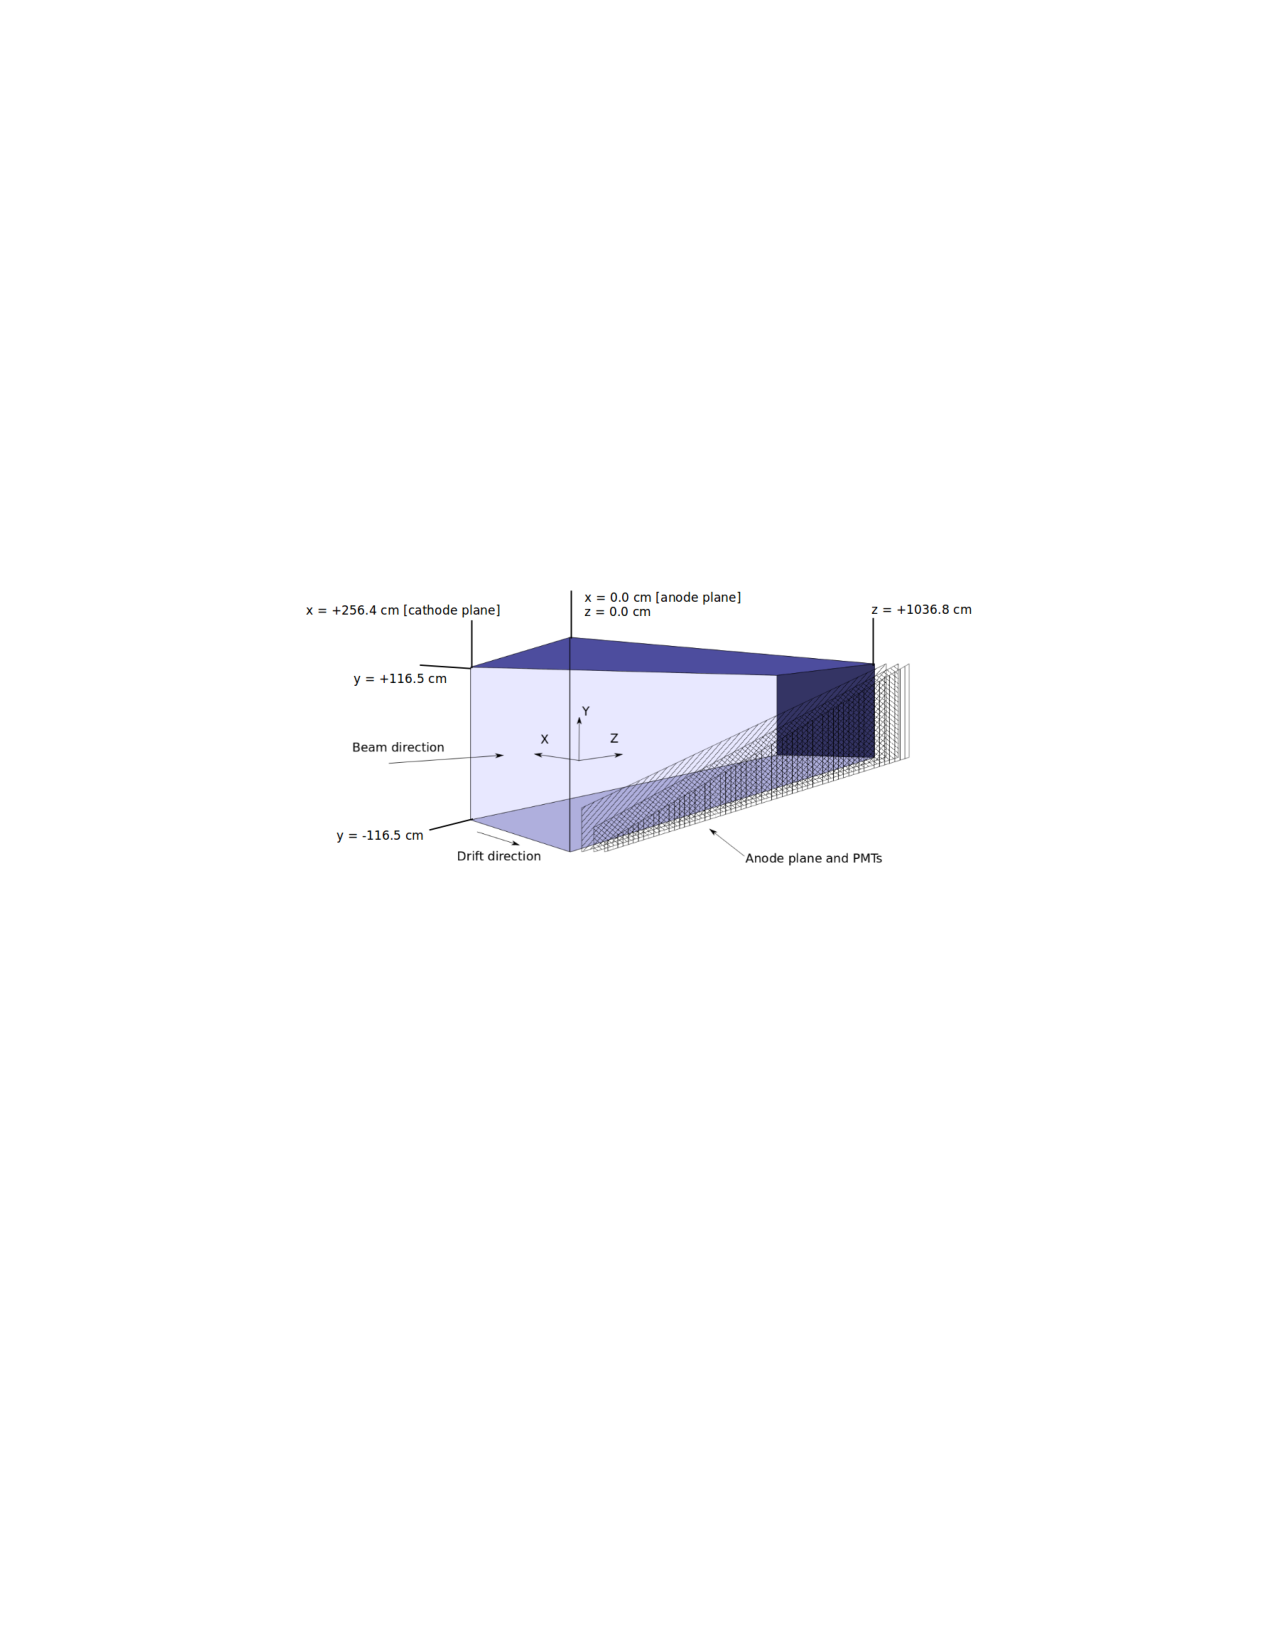
\includegraphics[width=0.95\linewidth]{figures/tpc_coordinates.pdf}
    \caption{Drawing of the MicroBooNE TPC showing the coordinate system and the size of each side. The anode and the cathode are respectively on the right and the left, as seen from the beam.}
    \label{fig:tpc_coordinates}
\end{figure}

MicroBooNE started acquiring neutrino data in October 2015. Figure \ref{fig:evd_ccpi0} shows the event display of a $\nu_{\mu}$ CC$\pi^0$ candidate in the collection plane. The excellent granularity of the detector allows appreciating the electromagnetic showers coming from a $\pi^0\rightarrow\gamma\gamma$ decay and also the small $\delta$-rays produced by the cosmic muons. It is also possible to appreciate the challenge of the pattern recognition, with different topologies and overlapping ionisation trails given by the presence of cosmic rays. 

\begin{figure}[htbp]
    \centering
    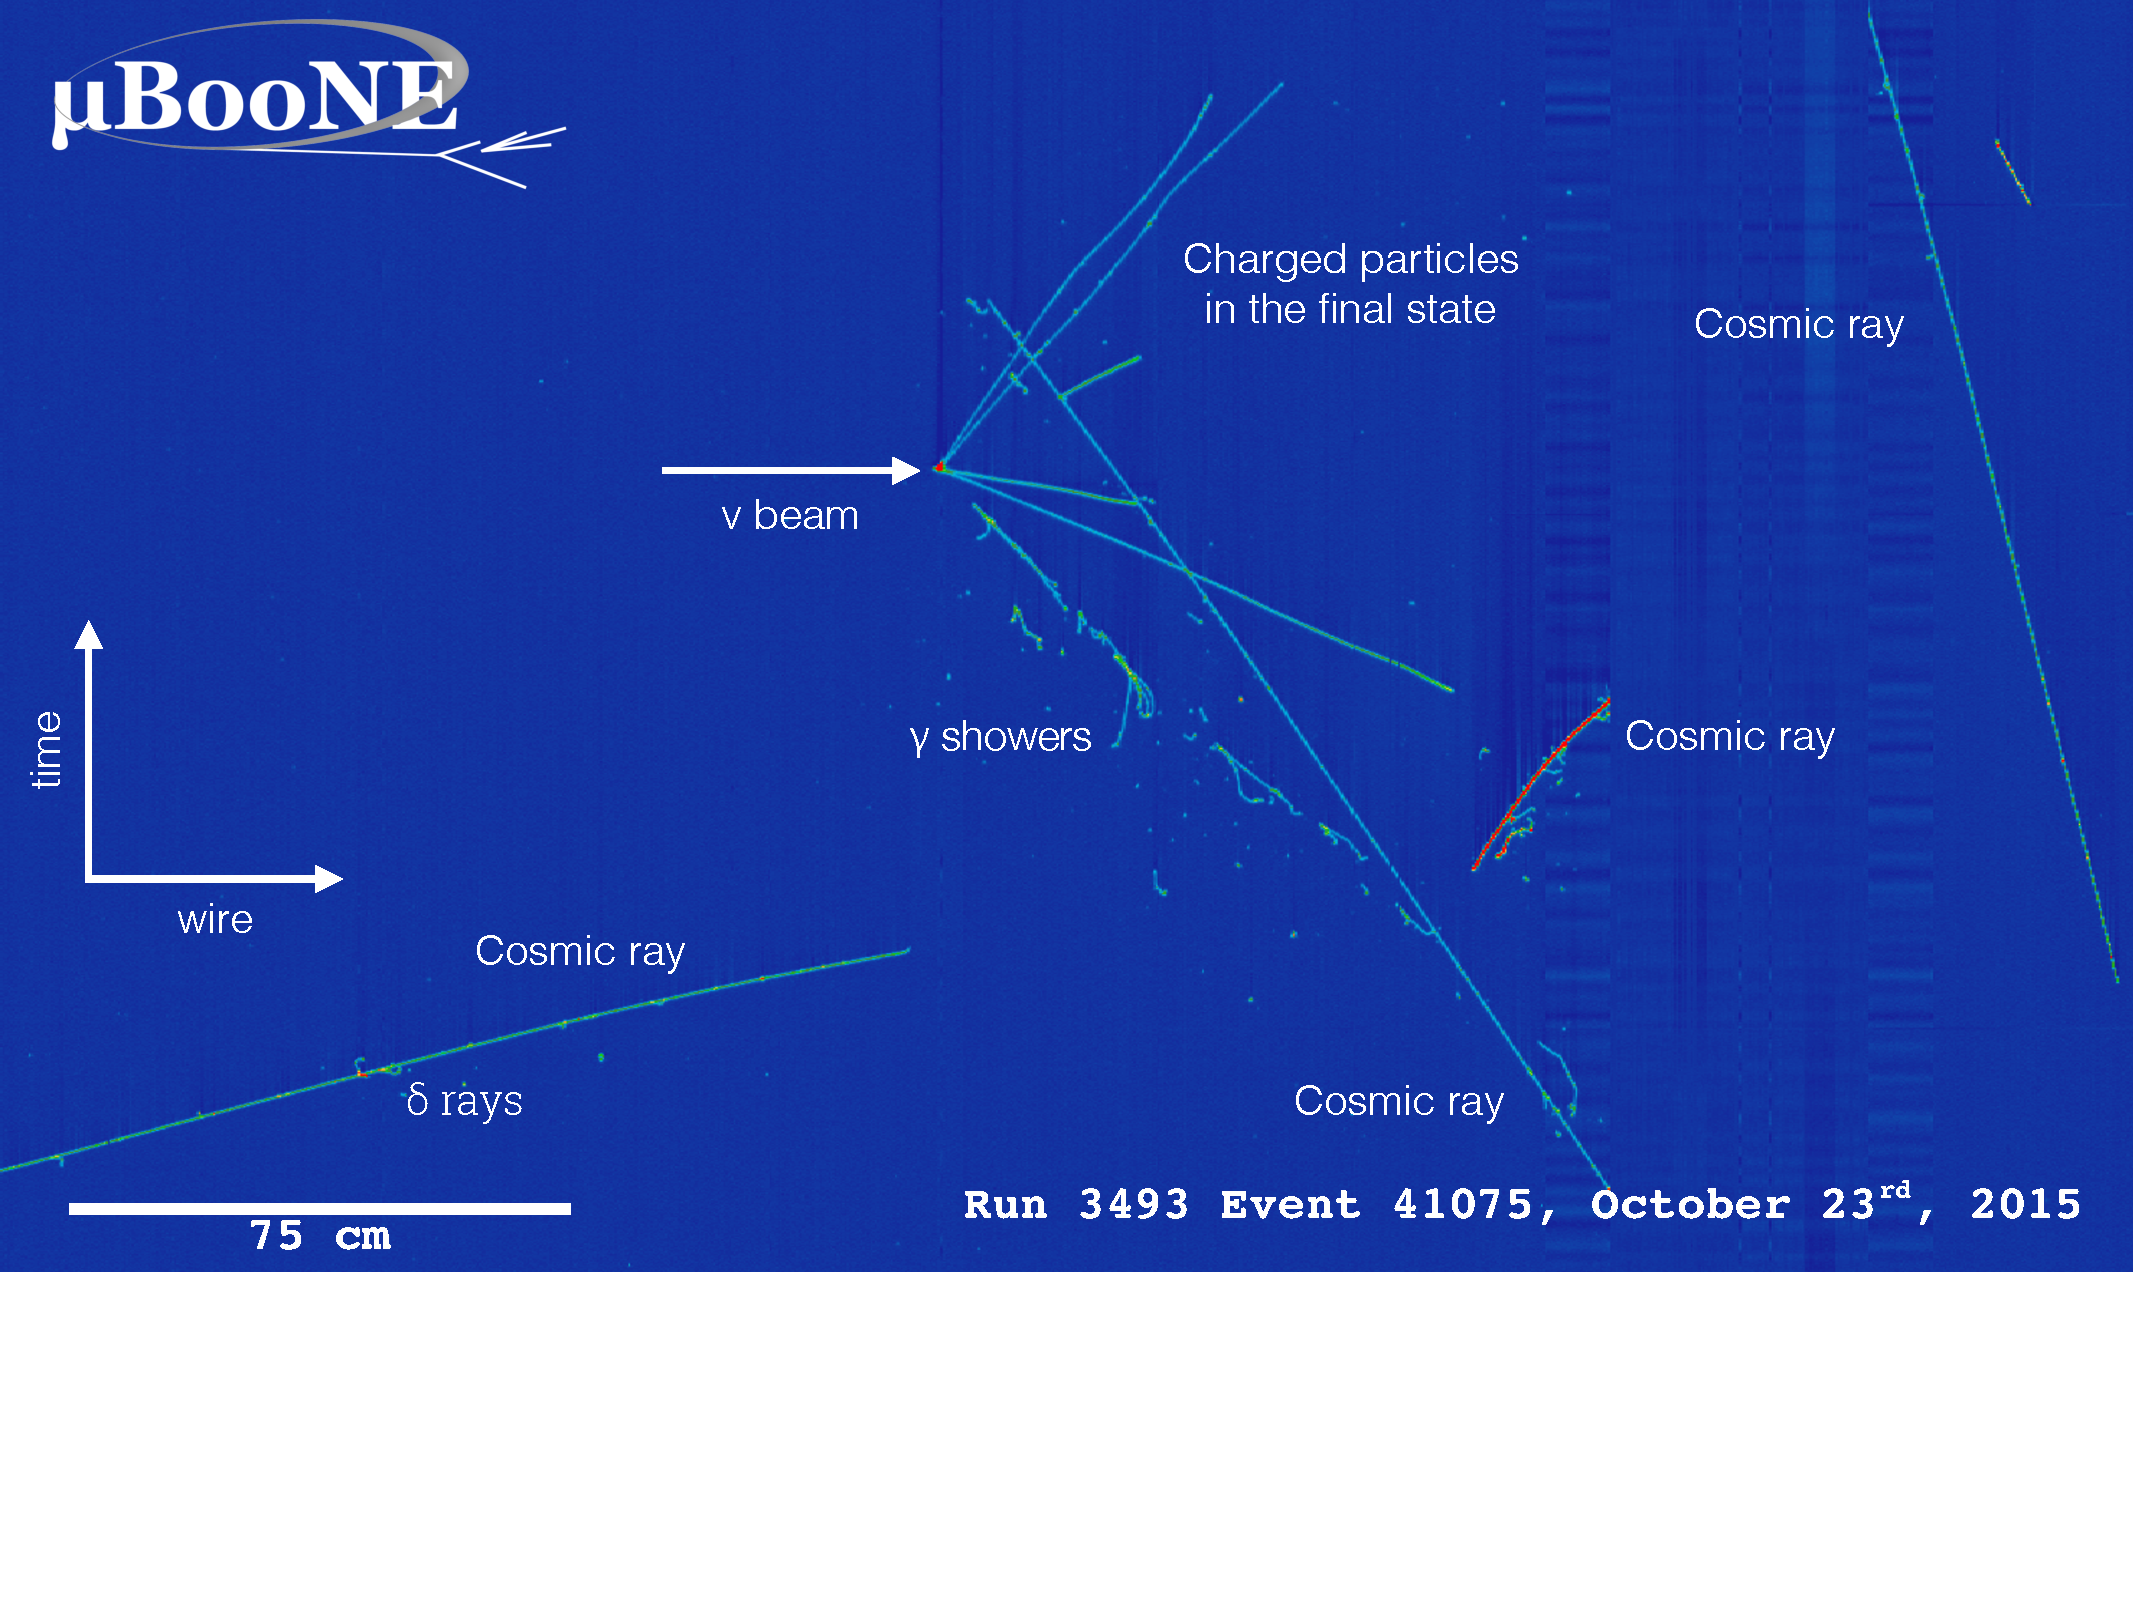
\includegraphics[width=0.9\linewidth]{figures/evd_ccpi0.pdf}
    \caption{Event display of a $\nu_{\mu}$ CC$\pi^0$ candidate in the collection plane. The colour scale corresponds to the amount of charged deposited on the wires.}
    \label{fig:evd_ccpi0}
\end{figure}


\subsection{The Light Collection system}
The MicroBooNE light collection system consists of 32 photomultipliers (PMTs) operating in the liquid argon and placed behind the anode plane, which is 86\% transparent to the light.
The liquid argon scintillation light has a typical spectrum peaked at 128~nm, which must be shifted to a higher wavelength region, where the PMTs have higher efficiency.
MicroBooNE employs tetraphenyl-butadiene (TPB), which absorbs in the UV and emits at $425\pm20$~nm. The efficiency for transmission through PMT borosilicate glass must also be taken into account (around 90\%).
Figure \ref{fig:light} summarises the light emission and absorption in the MicroBooNE light collection system.

\begin{figure}[htbp]
    \centering
    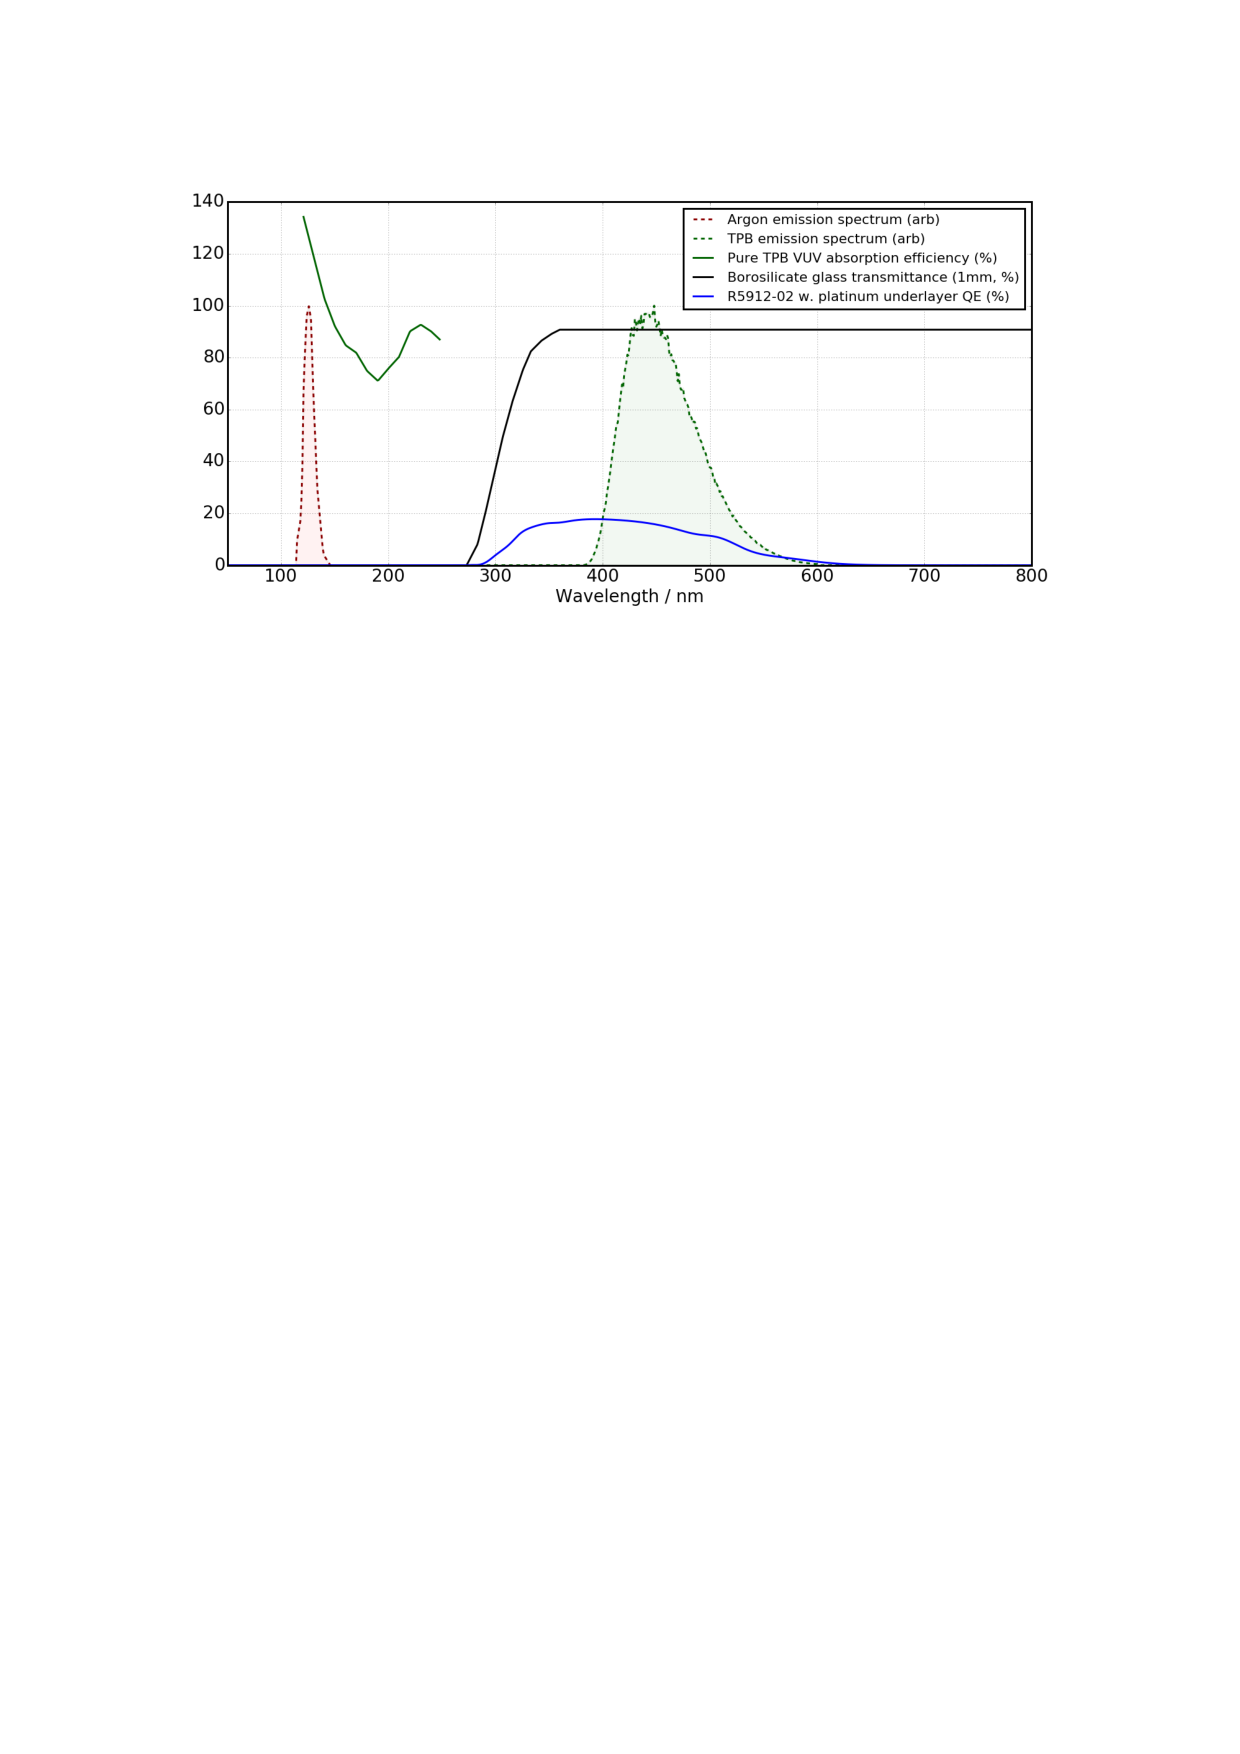
\includegraphics[width=0.85\linewidth]{figures/light.pdf}
    \caption{Scintillation light emission spectrum (red) and TPB re-emission spectrum (green), with the quantum efficiency of the PMTs employed in MicroBooNE (blue). PMT borosilicate glass transmittance is represented by the solid black line. From \cite{Acciarri:2016sli}.}
    \label{fig:light}
\end{figure}

\subsection{Cryogenics and purification}
The liquid argon needs to be kept at a constant temperature and pressure, since they strongly correlate with the drift velocity and, in turn, with the reconstruction of the $x$ coordinate.

The temperature is monitored by 12 Resistive Thermal Devices (RTDs) placed in various location of the cryostat, which is covered with insulating foam to prevent large temperature variations. 

The purification of the liquid argon is performed by a system of two condensers, two pumps, and two filters. The gaseous argon that leaves the detector enters a condenser kept at boiling temperature by liquid nitrogen coils (77~K) and it is then pumped into the filters which mainly remove water and O$_2$ molecules. The performances of the purification system can be quantified by measuring the electron lifetime ratio, as shown in Figure \ref{fig:purity}.

\subsection{Electronics and readout}
MicroBooNE readout electronics can be divided into two main parts: one responsible for the digitisation and recording of the TPC wire signals and one responsible for the digitisation and recording of the PMT signals. 

\paragraph{TPC readout and electronics}
The TPC electronics system can be classified into \emph{cold} electronics, placed inside the cryostat in the liquid argon and responsible for pre-amplification and shaping, and \emph{warm} electronics, placed outside the cryostat and responsible for digitisation and compression of the signals.

The pre-amplification and shaping of the signals happen in the ASIC CMOS chips on cold motherboards placed near the wires, in order to obtain the lowest possible noise. In particular, the wire noise is reduced by a factor of 2 when going from room temperature to liquid argon boiling temperature \cite{Chen:2012kv}. 

The signals are carried through warm wires to the Analog-to-Digital Converters (ADCs) boards and digitised by a 16 MHz clock. The waveforms are then processed in Front-End Modules (FEMs) and down-sampled to 2 MHz. The output consists of time-ordered waveforms of 9600 time-ticks, for a total of 4.8~ms.%, which is three times the drift-time window. 

\paragraph{PMTs readout and electronics}
The signals coming from the 32 PMTs are mainly used in MicroBooNE for the software trigger, as described in Section \ref{sec:trigger}, and to store information on the light emitted by the liquid argon scintillation.

Signals from the PMTs are first split by a dedicated circuit in a high-gain ($\sim20$~ADC/PE) and a low-gain ($\sim2$~ADC/PE) channel which carry 18\% and 1.8\% of the total signal amplitude, respectively.

Then, they are amplified and shaped with a 60~ns rise time and finally digitised at 64 MHz (15.625 ns time-tick). The waveforms are stored over a window of 1500 time-ticks (23.4~\si{\micro}s), starting 4~\si{\micro}s before the beam gate, which is 1.6~\si{\micro}s (10~\si{\micro}s) long for the BNB (NuMI beam). Digitised waveforms outside this window are stored only if above 130 ADC counts (around 6.5~PE) and for a duration of 40 time-ticks (0.6~\si{\micro}s), in order to reduce the data stream. A dead-time of 45 samples (0.7~\si{\micro}s) follows each recorded out-of-beam-gate digitised waveform.



\subsection{The MuCS and the Cosmic-Ray Tagger}\label{sec:crt}

Being located almost on surface, the MicroBooNE detector is constantly subject to a constant $\sim5.5$~kHz cosmic-ray rate \cite{Acciarri:2017rnj}, which corresponds to around 13 cosmic rays for a drift-time window of 2.3~ms. 

In order to study the challenges of cosmic-ray reconstruction, the MicroBooNE detector was also equipped with a small external muon counter stack (MuCS), installed at the start of operations in 2015. 

This sub-detector was used to measure for the first time the cosmic-ray reconstruction efficiency in a LArTPC. This measurement is described in detail in the publication reported in Appendix \ref{sec:mucs}, whose corresponding author is the author of this thesis. Triggering on the signal coming from this small muon counter stack allowed to measure the fraction of cosmic-ray tracks effectively reconstructed in the LArTPC. The measured efficiency is 97.1\%, in agreement with the Monte Carlo simulation. 

This study was also used to demonstrate the tagging capabilities of a larger Cosmic-Ray Tagger (CRT), which surrounds the cryostat on four sides and represents the first cosmic-ray tagging system integrated with a LArTPC \cite{Auger:2016tjc}. Figure \ref{fig:mucs_crt} shows a simulation of the cosmic rays which hit the LArTPC and are tagged by the MuCS and the CRT.

\begin{figure}[htbp]
\centering
  \begin{subfigure}{0.48\textwidth}
    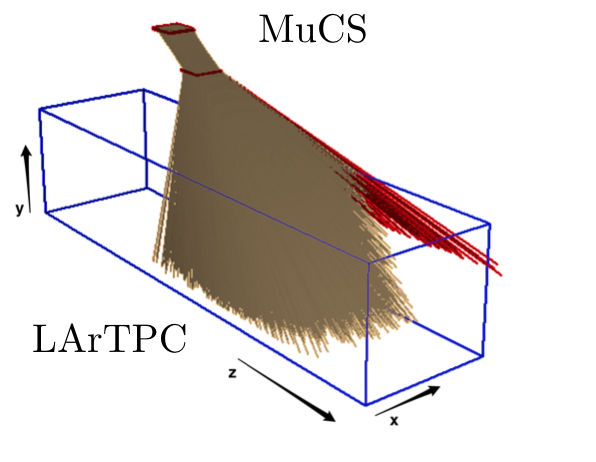
\includegraphics[height=0.7\linewidth]{figures/mucs.png}
    \caption{Cosmic rays hitting the MuCS. Red lines correspond to cosmic rays hitting the MuCS but missing the LArTPC.}
  \end{subfigure}\hfill
  \begin{subfigure}{0.48\textwidth}
    \begin{center}
        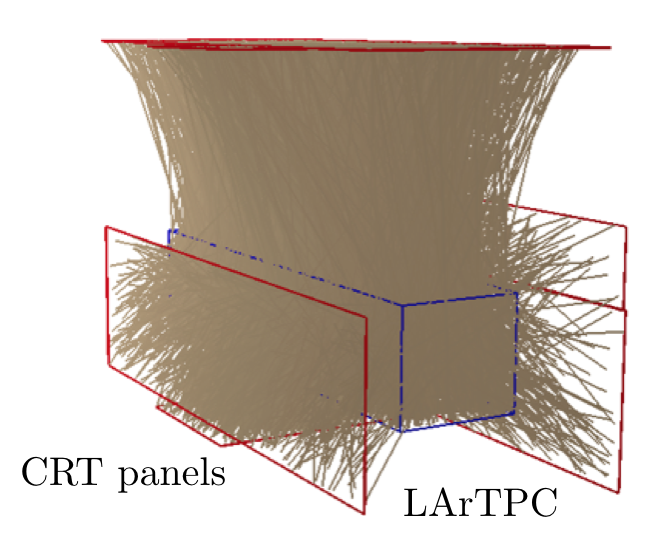
\includegraphics[height=0.7\linewidth]{figures/crt_panels.png}
        \caption{Cosmic rays hitting at least of the one of the CRT panels and the LArTPC.}
    \end{center}
  \end{subfigure}
    \caption{3D drawing of simulated cosmic rays (brown lines) hitting the LArTPC and tagged by the MuCS (left) and the CRT (right).}\label{fig:mucs_crt}
\end{figure}

This sub-system was installed at Fermilab in 2017 and was not present when the data used in this thesis was acquired. 

The CRT panels are made of plastic scintillation modules, which provide time and position information for charged particles crossing the panels and hitting the TPC.
Cosmic-ray rejection in the LArTPC can be improved both by spatially tagging crossing cosmic rays and by vetoing events with a signal in the CRT during the beam-gate window. 

\subsection{Trigger system}\label{sec:trigger}
MicroBooNE employs different triggers in order to minimise the amount of stored data, while keeping a very high neutrino efficiency.

A hardware trigger is fired for each beam spill in the Booster and in the NuMI neutrino beams. When received, a 23.4~\si{\micro}s window is opened in the PMT readout and a 4.8~ms window is opened in the TPC readout. These two triggers (one for the BNB and one for NuMI) have the highest priority, and in case the two beam-gate windows overlap, the precedence is given to the BNB. The beam trigger efficiency is 99.8\%.

Each event in MicroBooNE requires around 30~MB of storage which, for a 5~Hz beam-trigger rate, would correspond to 13~TB/day. However, most beam spills do not produce an effective neutrino interaction in the detector. In order to minimise the number of events containing only cosmic rays, thus reducing the amount of data stored, the beam trigger is required to be in coincidence with a PMT trigger, implemented at software level. In this way, it is possible to achieve a higher level of sophistication and makes the Monte Carlo simulation of the trigger easier. 

\begin{figure}[htbp]
    \centering
    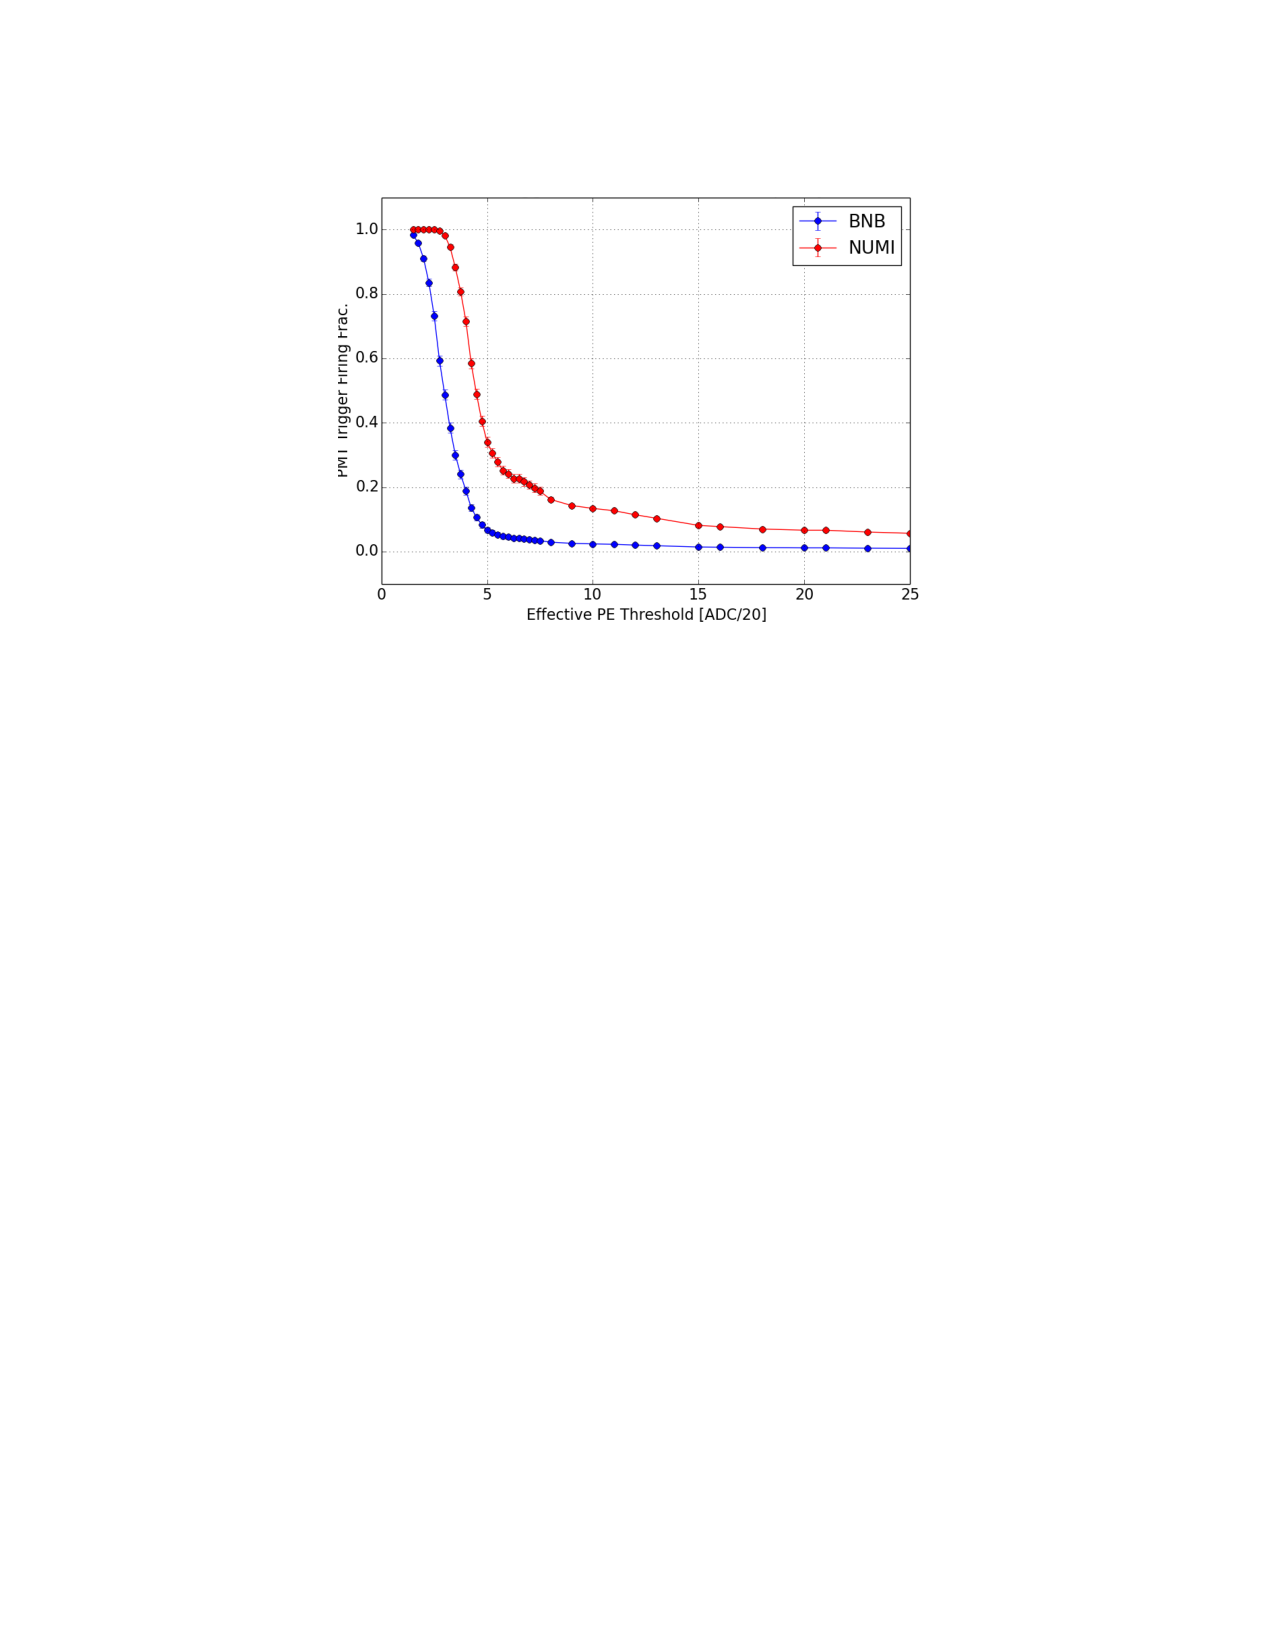
\includegraphics[width=0.85\linewidth]{figures/pmttrigger.pdf}
    \caption{Software trigger efficiency as a function of the PE threshold, both for BNB (blue) and NuMI (red) beam-gate windows.}
    \label{fig:pmttrigger}
\end{figure}

The software trigger requires 6.5 effective PE (photoelectrons) in the light collection system during the beam gate window, rejecting around 97\% of the beam spills. Figure \ref{fig:pmttrigger} shows the software trigger efficiency as a function of the PE threshold, both for BNB and NuMI beam-gate windows. \mccorrect{The NuMI beam trigger has a higher efficiency compared with the BNB beam trigger because the neutrinos are on average more energetic.}

Cosmic rays can still produce background events if they cross the TPC during the beam gate window, and produce enough scintillation light. In order to precisely assess this background, a trigger, called EXT, is fired at a 0.1~Hz rate orthogonally to the beam-gate windows, requiring 6.5 PE in a 1.6~\si{\micro}s time window (same as the BNB beam trigger). Events selected by this \emph{beam-off} trigger will then contain only cosmic rays.

Figure \ref{fig:trigger} shows the time-distribution of \emph{optical flashes} recorded from events triggered during the BNB beam-gate window. An optical flash is a group of light pulses recorded by the PMTs within a 100~ns time difference. The excess of events corresponds to the 1.6~\si{\micro}s beam spill width. 

\begin{figure}[htbp]
    \centering
    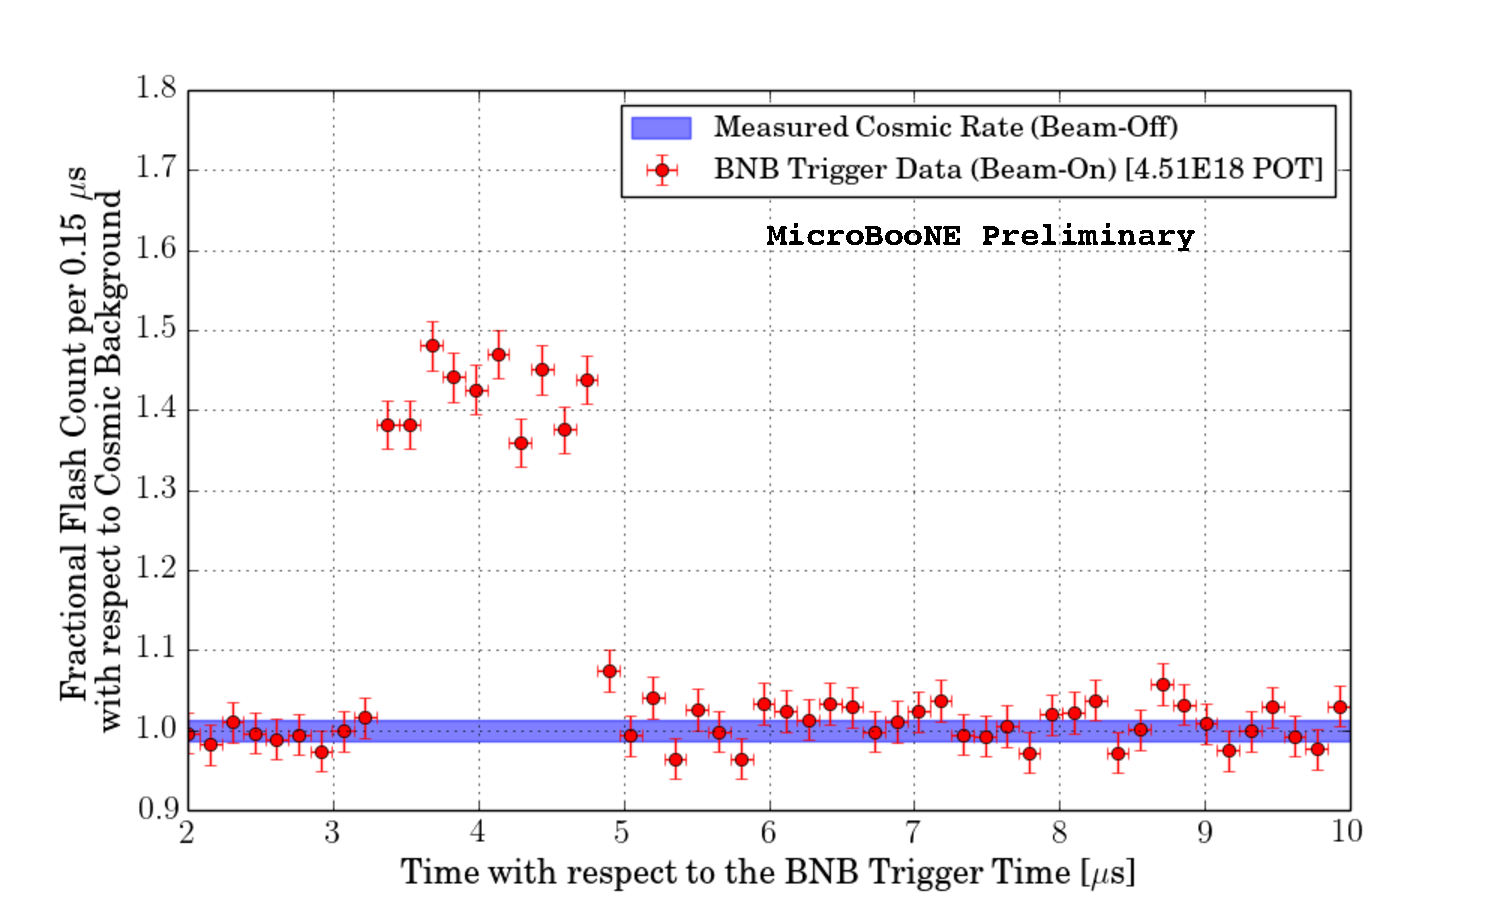
\includegraphics[width=0.85\linewidth]{figures/trigger.pdf}
    \caption{Distribution of optical flash times with respect to the trigger time for BNB triggered events, shown as a ratio to the expected cosmic rate from beam-off data, collected with the EXT trigger.}
    \label{fig:trigger}
\end{figure}

The DAQ (data acquisition) system takes as input the triggered TPC and PMT readouts and translates the raw data format into ROOT files, one for each trigger. As of January 2019, MicroBooNE has collected $1.2\times10^{21}$ POT in BNB neutrino mode, which roughly corresponds to the amount of POT collected by MiniBooNE (which collected also $1.1\times10^{21}$ POT in antineutrino mode and $1.9\times10^{20}$ POT in beam dump mode).
This document will focus on $4.34\times10^{19}$ POT collected with the BNB trigger between February 23 and May 22, 2016, which corresponds to MicroBooNE \emph{open data sample}. 
\chapter{Event reconstruction}\label{sec:eventreco}

\minitoc

In this section we will describe the process which transforms the raw digitised waveforms collected by the DAQ into high-level objects used for physics analysis. 

\section{Signal processing}
\subsection{Noise removal}
The ASIC chips placed in the liquid argon produce an inherent irreducible noise, caused by thermal fluctuations and charge trapping and de-trapping in the input transistor \cite{Acciarri:2017sde}. 

However, MicroBooNE is also affected by excess noise beyond the expected inherent one. This excess noise has three main sources, whose identification and mitigation is thoroughly described in \cite{Acciarri:2017sde}. Here we provide a brief overview for informative reasons.
\begin{description}
\item[Noise induced by the low-voltage regulators.] The low-voltage regulators which feed the ASIC chips introduce a noise across all channels at around 30~kHz in the frequency spectrum. This component represents the most significant excess noise source. To mitigate it, a \emph{correction waveform} is constructed on a per sample basis and subtracted from each channel.
\item[HV power supply noise.] This noise is induced by the cathode high-voltage power supply around 36 kHz and 108 kHz. An offline filter directly removes this harmonic noise in the frequency domain.
\item[900 kHz burst noise.] The source of this noise is still unknown. It is position-dependent and has a burst nature. The main hypothesis points towards the PMT high-voltage supply. This noise is attenuated by the anti-alias filter and at the moment is not actively mitigated.
\end{description}
The entire noise-reduction filtering chain allows to increase the peak signal-to-noise ratio by a factor of 2 in the collection plane (from 19.5 to 37.9) and by a factor of 3 in the induction planes (from 6.6 to 22.3 in the U induction plane and from 5.7 to 16.2 in the V induction plane). As an example, Figure \ref{fig:evd_noise} shows an event display of the V induction plane before and after the noise removal: a clear neutrino interaction emerges with the improvement in the signal-to-noise ratio. 

\begin{figure}[htbp]
    \centering
    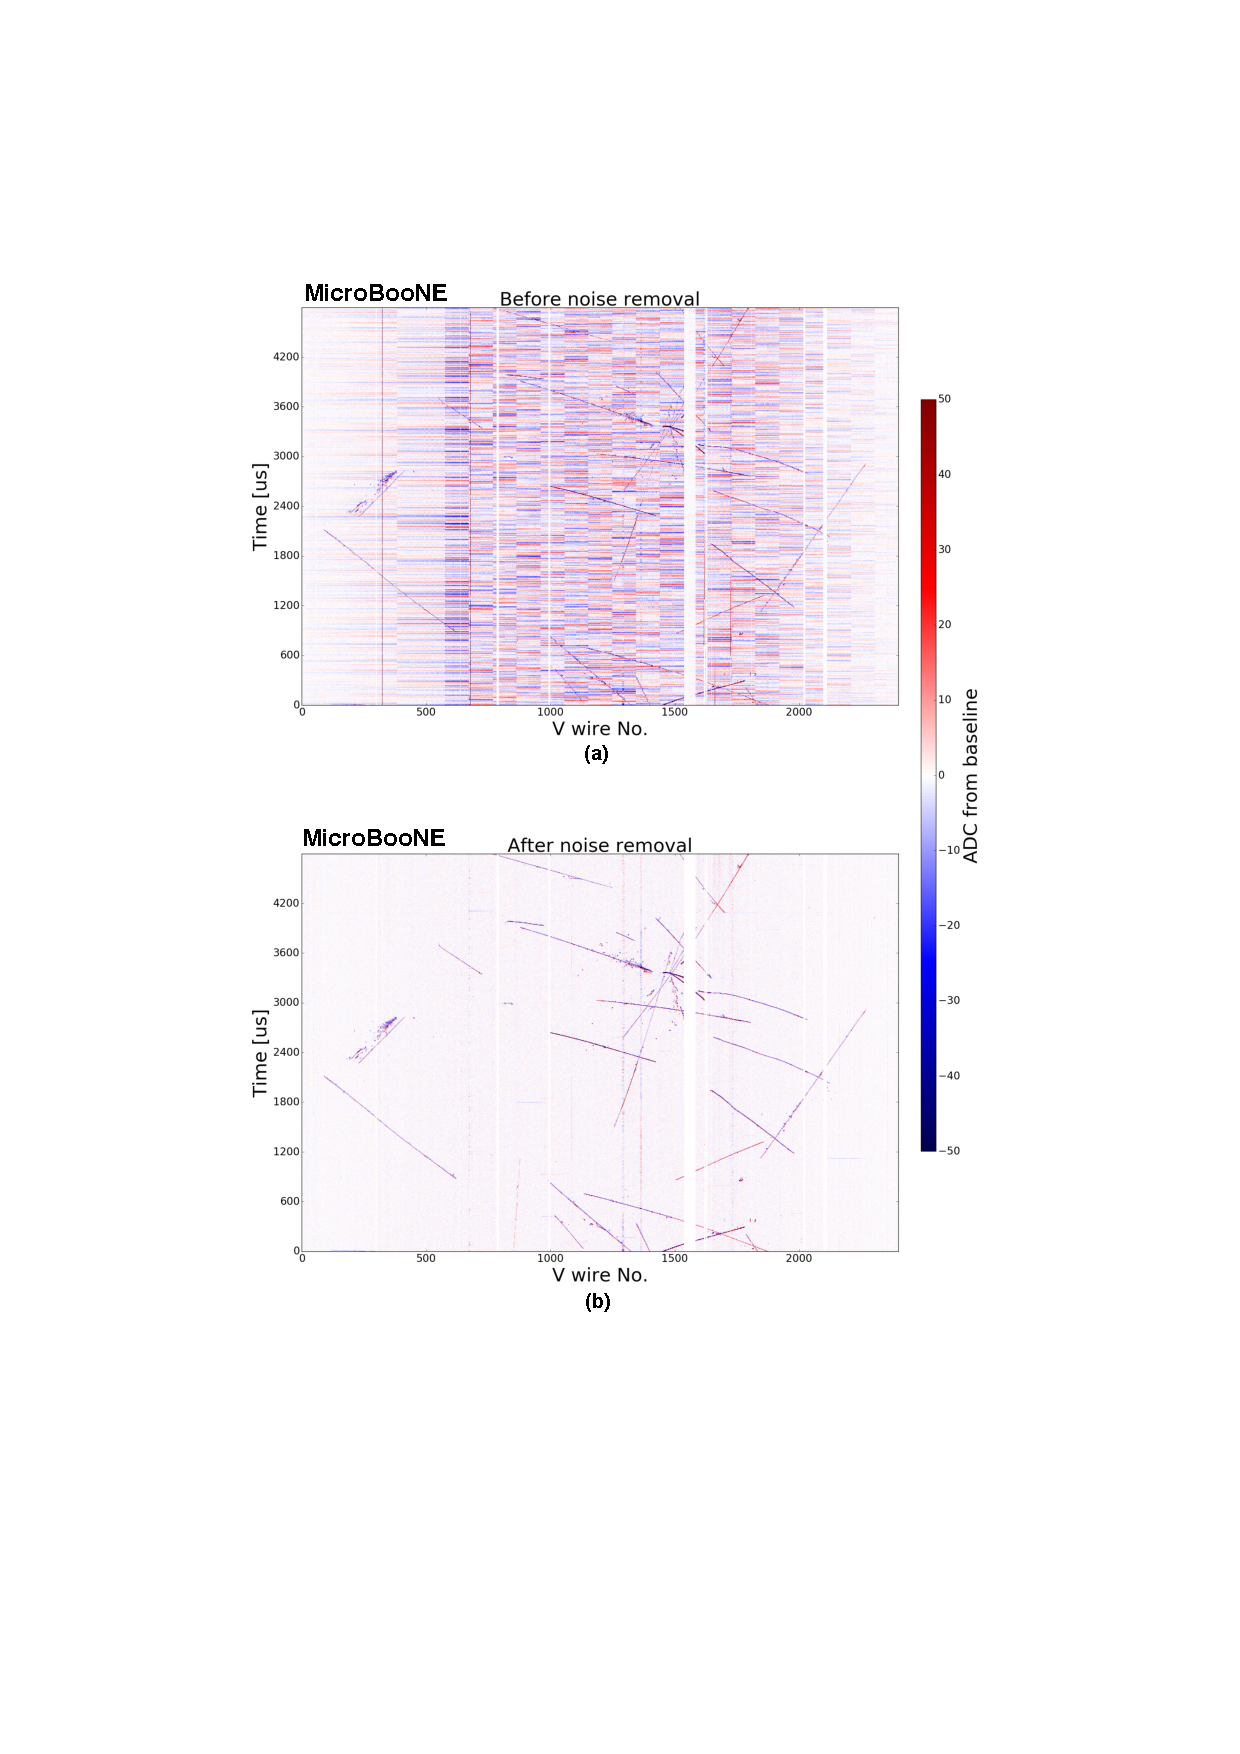
\includegraphics[width=0.75\linewidth]{figures/evd_noise.pdf}
    \caption{Data event display of the V induction plane showing the raw signal before (a) and after (b) offline noise filtering. From \cite{Acciarri:2017sde}.}
    \label{fig:evd_noise}
\end{figure}

\subsection{Signal deconvolution}
After the noise-filtering stage, a first reconstruction step searches for regions-of-interest (ROI) in the wire signals. Thus, the signal deconvolution step aims to disentangle the detector electronic response from the original profile of the charge collected or induced on the wires. This process is usually performed with a Fourier transform of the measured signal, which yields:
\begin{equation}
    S(\omega) = \frac{M(\omega)}{R(\omega)},
\end{equation}
where $S(\omega)$ is the original signal, $M(\omega)$ is the measured signal, and $R(\omega)$ is the response function, all in the frequency domain. However, the response function typically decreases at high frequencies, leading to increased noise in this region of the frequency domain. This issue is solved by applying a filter function $F(\omega)$, whose details are thoroughly described in \cite{Adams:2018dra}. 

\subsection{Hit reconstruction}
The final stage of the signal processing tries to perform one or more Gaussian fits to the deconvolved signals. Each Gaussian fit corresponds to a \emph{reconstructed hit}. The time of the reconstructed hit is the mean of the Gaussian and its RMS corresponds to the Gaussian width. The integral of the fitted function gives the charge associated to the hit. Figure \ref{fig:evd_wires} shows a data event display of the collection plane, with two peaks in the ROI, produced by the ionisation trails of two cosmic rays. 
These reconstructed hits are finally passed to the pattern recognition framework, which aims to reconstruct 2D and 3D clusters. 

\begin{figure}[htbp]
    \centering
    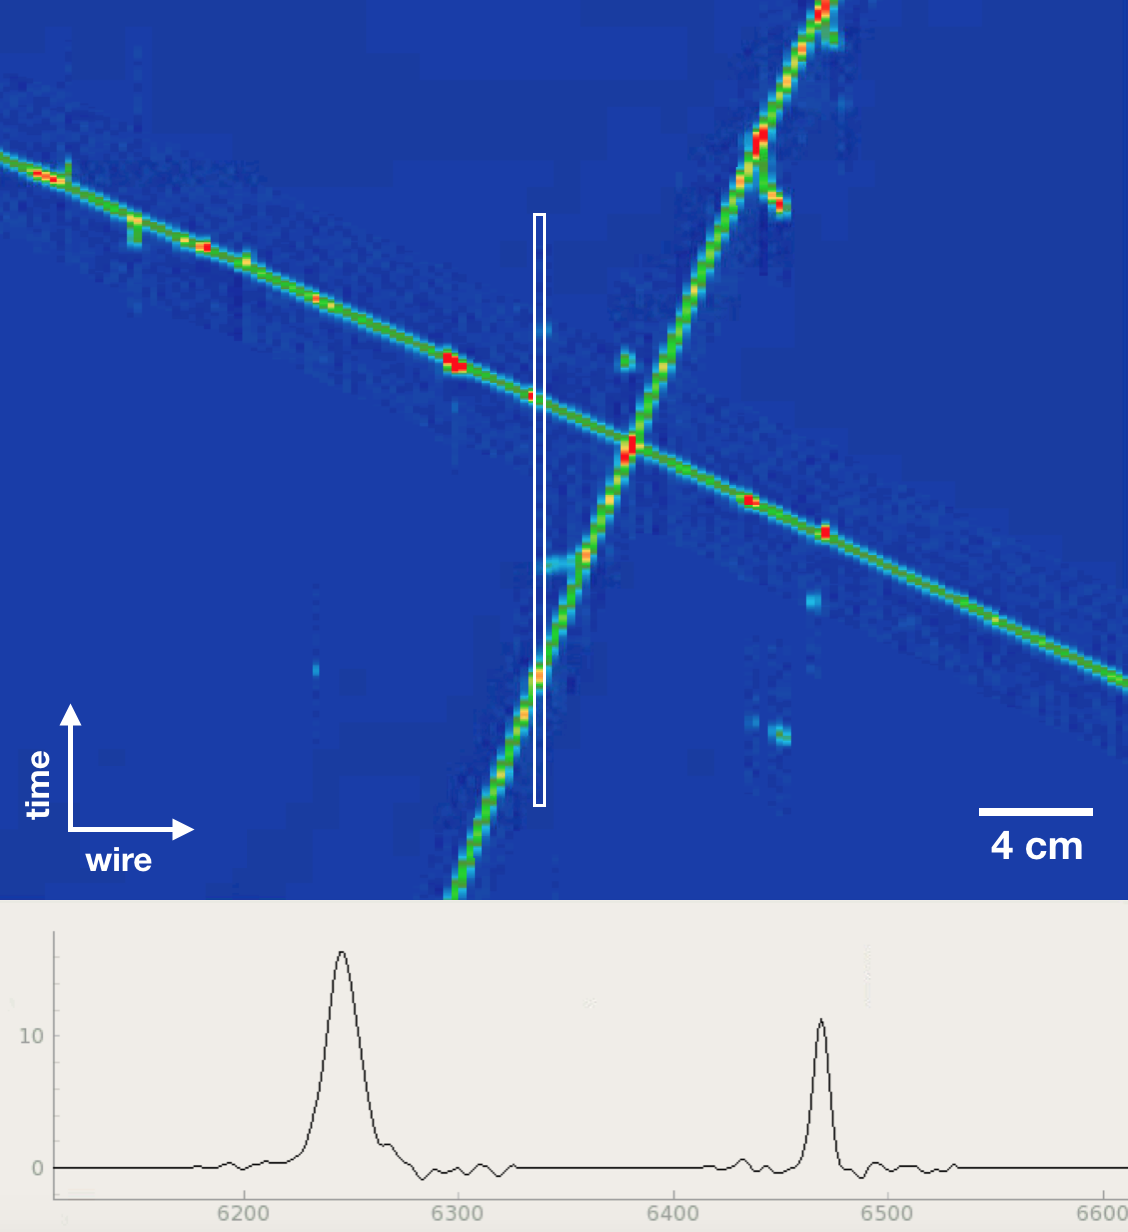
\includegraphics[width=0.75\linewidth]{figures/evd_wires.png}
    \caption{Data event display with the waveform collected in a wire of the collection plane. The white box corresponds to the waveform in the bottom part. The units of the x-axis are in 500 ns time-ticks.}
    \label{fig:evd_wires}
\end{figure}

\section{The Pandora multi-algorithm pattern recognition}
The results shown in this document were produced using the Pandora Software Development Kit for pattern recognition. This general-purpose framework was specifically developed to identify energy deposits in high-granularity detectors, such as LArTPCs \cite{Marshall:2015rfa}.

Several algorithms are applied in sequence to the input information (in our case the reconstructed hits), which gradually build up a complete picture of the event.

As a first step, input hits are separated into three different lists, one for each plane. Then, for each list, an algorithm group together continuous and unambiguous lines of hits. These two-dimensional clusters are then examined by a series of topological algorithms. Given the presence of missing or unresponsive wires in the MicroBooNE detector, a continuous ionisation trail can be reconstructed as two or more separate clusters. The topological algorithms try to stitch different clusters together, if e.g. they point towards the same direction or if they are in close proximity. 

\begin{figure}[htbp]
    \centering
    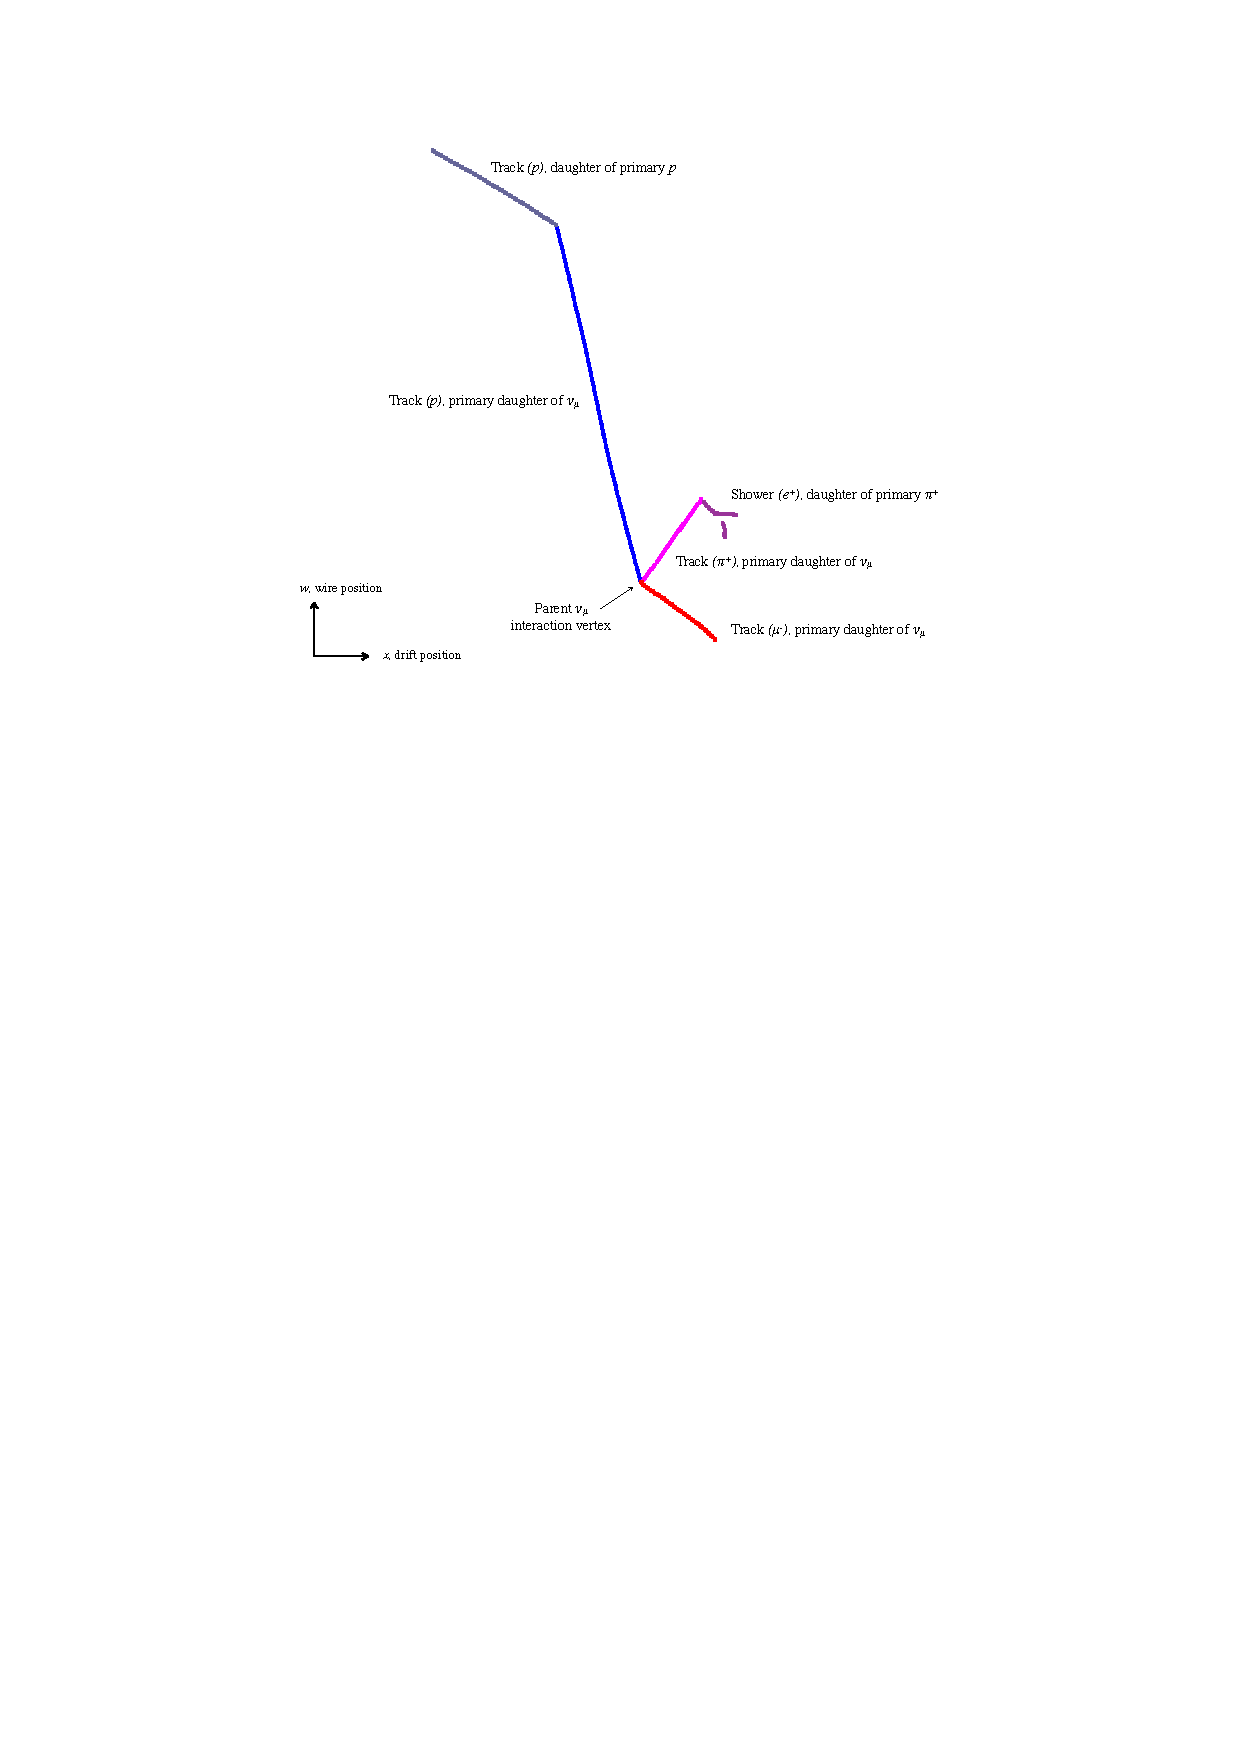
\includegraphics[width=0.75\linewidth]{figures/pandora_evd.pdf}
    \caption{Pandora pattern recognition output of a simulated CC $\nu_{\mu}$ event with a muon, a proton and a charged pion in the final state. Each particle is reconstructed as a separate cluster and the positron coming from the $\pi^+\rightarrow\mu^+\rightarrow e^+$ decay chain is classified as a daughter of the pion. From \cite{Acciarri:2017hat}.}\label{fig:evd_pandora}
\end{figure}

Once the topological algorithms deem the clustering in each plane as complete, the 3D reconstruction algorithms take as input the clusters from the three planes and aim to reconstruct the three-dimensional objects, which in Pandora are called \emph{PFParticles}.
Subsequently, a Support Vector Machine trained on Monte Carlo uses the topological and geometrical properties of the object to classify it as \emph{track} or as a \emph{shower}. 
An important feature of the Pandora pattern recognition is its ability to create a hierarchy of reconstructed PFParticles. As an example, the reconstructed shower corresponding to a Michel electron will be considered as the daughter of the reconstructed track corresponding to the stopping muon. This capability is particularly important for the reconstruction of complex neutrino interactions, as exemplified in Figure \ref{fig:evd_pandora}.

Pandora can also run in two modes: one optimised for the reconstruction of cosmic rays and one optimised for the reconstruction of neutrino interactions. These two modes are used sequentially in our analysis in order to suppress the cosmogenic background, as described in Section \ref{sec:cosmicremoval}.
\chapter{Selection of electron neutrinos in the MicroBooNE experiment}\label{ch:6-analysis}

\minitoc

One of the main physics goals of the MicroBooNE experiment is to search for and clarify the low-energy excess of electron-like events observed by the MiniBooNE experiment \cite{Aguilar-Arevalo:2018gpe}. 

However, the MiniBooNE experiment employs a Cherenkov detector, which does not have the ability to distinguish between single electrons and single photons in the final state. This technology limitation makes it very challenging to identify a physics model that could definitely explain the excess.

The MicroBooNE detector, being a LArTPC, provides detailed  calorimetry, which makes it possible to measure the $dE/dx$ of ionisation tracks and electromagnetic showers \cite{Acciarri:2016sli}, and excellent granularity, which allows to measure the gap between the neutrino interaction vertex and the start of the electromagnetic shower. These two methods provide powerful electron/photon separation.% and are not normally available in a Cherenkov detector. 

In this chapter we will describe a fully-automated electron neutrino selection using the Pandora multi-algorithm pattern recognition. This is the first fully-automated electron neutrino search in MicroBooNE. The selection will be validated with two orthogonal side-bands and with an independent sample of events acquired with the NuMI beam. The systematic uncertainties will evaluated in Chapter \ref{sec:systematics} and the current sensitivity to the MiniBooNE low-energy excess in the electron hypothesis will be estimated in Chapter \ref{sec:sensitivity}.

\section{Signal definition}
The MiniBooNE experiment showed an excess of CCQE-like events in the 200-475~MeV neutrino energy range \cite{Aguilar-Arevalo:2018gpe}, therefore this analysis will focus on a similar topology.

Our selection aims to have a sample with one electron, no other leptons or photons, at least one proton, and no other charged hadrons or mesons in the final state. All particles in the final state are required to be above detection thresholds, evaluated in Section \ref{sec:eff}. These events are called $\nu_{e}$ CC0$\pi$-Np (where N > 0) \cite{Katori:2013nca}. 

In MicroBooNE, a $\nu_{e}$ CC0$\pi$-Np interaction corresponds to an electromagnetic shower, produced by the electron, and one or more ionisation tracks, produced by the protons.

The channel closest to the \emph{CCQE-like} events selected by MiniBooNE is CC0$\pi$ (so including events with 0 protons), since the Cherenkov threshold for protons in mineral oil is 350~MeV (kinetic energy) \cite{Perevalov:2009mn}.
However, the choice of the CC0$\pi$-Np channel presents several advantages, described below.
\begin{description}
    \item[Easier pattern recognition.] The presence of a proton in the final state makes vertexing and pattern recognition easier, since there will be typically a \emph{kink} between the ionisation track and the electromagnetic shower.
    \item[Improved energy resolution.] As shown in Section \ref{sec:energyreco}, the length of the ionisation tracks can be used to estimate the energy deposited by the protons. This method provides a higher energy resolution than the one obtained by collecting the deposited charge.
    \item[Improved background rejection.] Requiring an ionisation track allows to reject NC$\pi^0$ and CC$\pi^0$ interactions with no protons in the final state and where one of the $\pi^0\rightarrow\gamma\gamma$ is not reconstructed or escapes the detector. These events represent a large background of our analysis. Also, the presence of the proton allows to reject events with a photon converting far from the interaction vertex, as it makes possible to measure the gap between the shower and the interaction vertex.
\end{description}


As an example, figure \ref{fig:evd} shows a simulated $\nu_{e}$ CC0$\pi$-Np event display on the collection plane with an electron and two protons in the final state, with the corresponding reconstructed shower and reconstructed tracks. In this case, the patter recognition is able to correctly identify the electromagnetic shower and both proton tracks.

\begin{figure}[htbp]
	\begin{center}
    	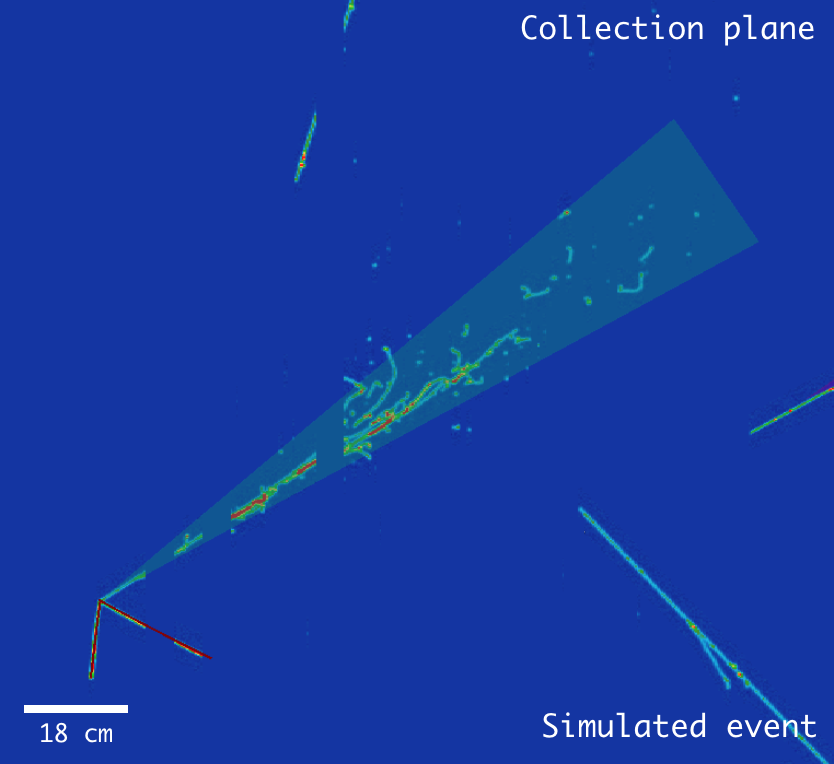
\includegraphics[width=0.85\linewidth]{figures/evd.png}
    	\caption{Monte Carlo $\nu_{e}$ CC0$\pi$-Np event display of the collection plane with an electron and two protons in the final state. The reconstructed shower-like object is represented by the green cone. The reconstructed track-like objects are represented by the red lines. The ionisation trails without an associated reconstructed track are cosmic rays correctly tagged by the cosmic-removal algorithms, described in Section \ref{sec:cosmicremoval}. The colour scale is proportional to the amount of charge collected by the wires. {The vertical gaps are caused by the presence of unresponsive wires in the detector, which are turned off in the simulation.}} \label{fig:evd}
	\end{center}
\end{figure}



\section{Analysis Methodology}
\label{sec:methodology}
The goal of the event selection is to obtain a sample enriched with $\nu_{e}$ CC0$\pi$-Np interactions. The results of the event selection are described in detail in Section \ref{sec:numu}. In order to increase the purity, two parallel background rejection strategies have been developed: one with rectangular cuts on kinematic and calorimetric variables, described in Section \ref{sec:cuts}, and one with Boosted Decision Trees, described in Section \ref{sec:bdt}.
The measurement of the systematic uncertainties affecting the variables used in the background rejection is described in Chapter \ref{sec:systematics}. The full covariance matrix has then be used to measure the sensitivity to the MiniBooNE low-energy excess signal in the electron hypothesis, in Chapter \ref{sec:sensitivity}.

\subsection{Data and Monte Carlo samples}\label{sec:data}
In this document, we will analyse a sub-sample of the data collected by the detector between February 23 and May 22, 2016. This sub-sample corresponds to an exposure of the MicroBooNE detector of \num{4.34e19} POT. This represents MicroBooNE unblinded sample for reconstruction, event selection development, and performance measurement. The sample is statistically too small to be sensitive to a MiniBooNE-like low-energy excess signal. 
%The entire dataset will be open once we are satisfied with the reconstruction, analysis chain, and future sensitivity estimates.

The data used for this analysis correspond to two separate samples: the \emph{data beam-on}, obtained with the BNB beam trigger, and the \emph{data beam-off}, obtained with the EXT trigger. These two triggers criteria were described in Section \ref{sec:trigger}.

In order to increase the simulated statistics of our $\nu_e$ CC0$\pi$-Np events, three different Monte Carlo samples were produced:
\begin{description}
\item[$\nu_{e}$ CC0$\pi$-Np + cosmic sample.] Each event has a simulated $\nu_{e}$ interaction in the MicroBooNE cryostat and simulated cosmic rays hitting the detector in the same readout window. The interaction is defined as $\nu_{e}$ CC0$\pi$-Np if it has one electron, at least one proton, no photons, and no mesons (pions, kaons) above detection threshold. The start and end points of the protons and the start point of the electron are required to be contained within the fiducial volume, as defined in Section \ref{sec:precuts}. This sample will be used to assess the reconstruction efficiencies of the analysis.
\item[BNB + cosmic sample.] Each event has a simulated neutrino interaction inside the MicroBooNE cryostat, where the neutrino flavours are weighted according to the BNB neutrino flux composition (see Section \ref{sec:beam}), and simulated cosmic rays hitting the detector in the same readout window. This sample will be used to understand backgrounds coming from other neutrino interactions.
\item[Dirt sample.] Each event has a simulated neutrino interaction outside the MicroBooNE cryostat, where the neutrino flavours are weighted according to the BNB neutrino flux composition, and simulated cosmic rays hitting the detector in the same readout window. This sample will be used to understand background events coming from interactions outside the fiducial volume.
\end{description}

Neutrino events have been generated using the GENIE Neutrino Monte Carlo generator version 2.8.6 \cite{Andreopoulos:2009rq} and cosmic rays have been generated using the CORSIKA Monte Carlo generator version 7.4003 \cite{Heck:1998vt}. Simulated secondary particle propagation employs GEANT version 4.9.6 \cite{Brun:1994aa}, and detector response simulation and reconstruction is performed with the LArSoft framework version 6.26.01.10 \cite{Church:2013hea}.

\subsection{Overview of the analysis}
The reconstruction and selection chain to identify $\nu_{e}$~CC0$\pi$-Np electron neutrino candidate events for this analysis is divided into several stages:

\begin{description}
\item[Cosmic-ray removal.] In order to suppress the cosmogenic background, the first step is to rune the Pandora algorithms optimised to reconstruct and remove cosmic rays \cite{Acciarri:2017hat}. After this step, hits associated with objects deemed as cosmic-induced by several tagging algorithms, external to Pandora and described in Section \ref{sec:cosmicremoval}, are removed from the event. The remaining hit collection provides the input to the Pandora neutrino reconstruction path, which outputs a list of candidate neutrinos.

\item[Optical selection.] A minimum amount of coincident photoelectrons in the optical detection system is required to be coinciding with the BNB beam window and at least one of the neutrino candidates provided by the Pandora framework must be compatible with the flash observed in the optical detection system. These requirements are described in detail in Section \ref{sec:optical_pre_cuts}.

\item[Electron neutrino topological pre-selection.] One of the neutrino candidates must be compatible with the topology of a $\nu_{e}$ CC0$\pi$-Np interaction. Rather than accepting strictly $N$ tracks and one shower, at least one track and at least one shower or at least two showers sharing a common vertex are accepted, due to the presence of split showers and split tracks. Multiple showers without reconstructed tracks are accepted due to a current track/shower identification inefficiency, addressed in Section \ref{sec:ineff}.

\item[CC $\nu_{\mu}$ neutrino candidates removal.] Events tagged as CC $\nu_{\mu}$ neutrino candidates are rejected by an independent CC $\nu_{\mu}$ selection module, described in \cite{ubxsec}. 

\item[Calorimetric variables reconstruction.] The energy of the electron showers is measured with a calorimetric procedure, converting the collected charge into deposited energy, while the energy deposited by the proton tracks is calculated from the length of the reconstructed track. The $dE/dx$ of the ionisation tracks and electromagnetic showers is also measured for particle identification purposes and are detailed in Section \ref{sec:energyreco}.

\item[Background rejection.] The $\nu_{e}$~CC0$\pi$-Np events can be further isolated by applying a suite of cuts on kinematic, geometric, and calorimetric variables. The electromagnetic showers initiated by an electron in the final state are isolated with a cut on the $dE/dx$ value and the proton tracks are selected with a cut on the $\chi^{2}$ score of their $dE/dx$ vs. residual range profile. An alternative background-rejection strategy has also been developed using Boosted Decision Trees. These are described in Sections \ref{sec:cuts} and \ref{sec:bdt}.
\end{description}

A schematics of the event selection stages is shown in Figure \ref{fig:selection}.

\begin{figure}[htbp]
\centering
  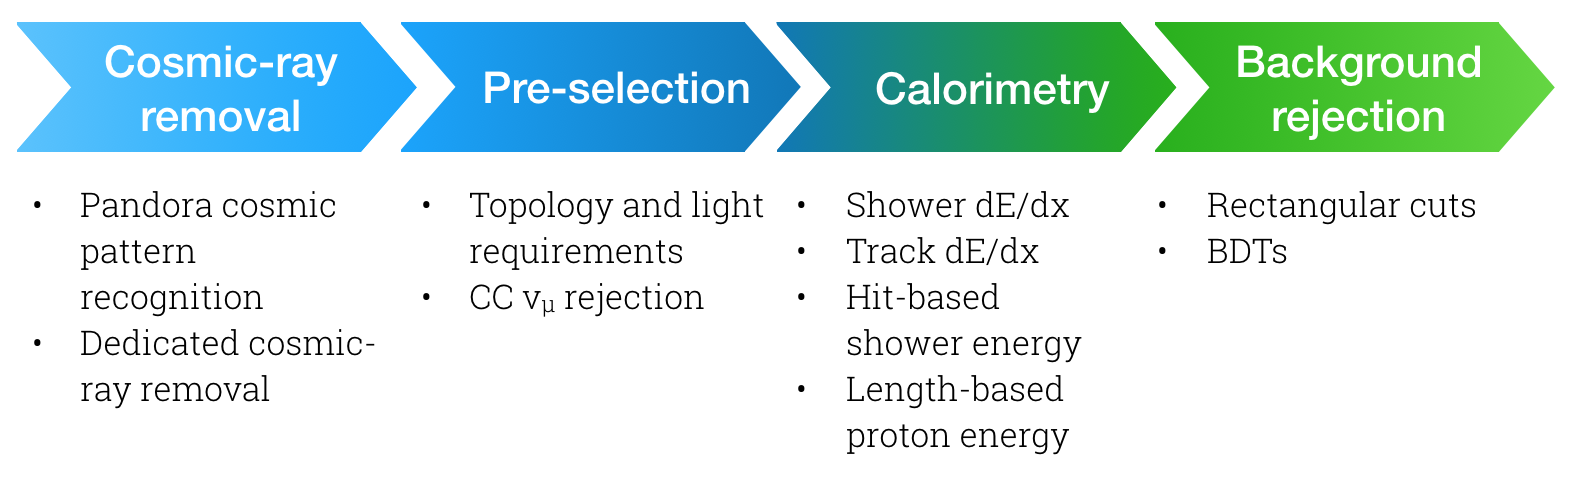
\includegraphics[width=0.9\linewidth]{figures/selection.png}
  \caption{Schematics of the $\nu_e$ CC0$\pi$-Np event selection stages, from the cosmic-ray removal to the rejection of the neutrino and cosmogenic backgrounds.}
  \label{fig:selection}
\end{figure}

\subsection{Cosmic-ray rejection}\label{sec:cosmicremoval}
The hits in the TPC, reconstructed with the procedure described in Section \ref{sec:eventreco}, are passed to the Pandora framework for pattern recognition. %The framework can run in two different modes: one optimised for the reconstruction of cosmic rays and delta rays (\emph{cosmic mode}), and one optimised for the reconstruction of neutrino interactions (\emph{neutrino mode}).

In order to reject the cosmogenic background, Pandora is first run in cosmic mode over all the reconstructed hits. This reconstruction is track-oriented, and the delta rays are reconstructed as showers and considered as daughters of the closest cosmic muon. The starting point of the reconstructed tracks in this mode is assumed to be the highest $y$ coordinate \cite{Acciarri:2017hat}.
These reconstructed high-level objects are fed to a series of cosmic-ray tagging algorithms, which are briefly described below.
\begin{description}
\item[Geometry and timing algorithm.] This algorithm checks if the reconstructed hits have a time compatible with the drift-time window. If a track or a shower has more than four hits outside the allowed drift-time window, then they are tagged as cosmic rays. Then, the algorithm loops over all the reconstructed objects and tag them if they have a trajectory that enters and exits the TPC borders, within a fiducial volume. The fiducial volume has been chosen by taking into account the magnitude of the space charge effect (Section \ref{sec:ionisation}).
\item[Flash-matching algorithm.]{This algorithm takes into account the information provided by the optical system to reject cosmic rays interacting during the readout window. The algorithm first requires the presence of a reconstructed flash during the beam-spill window of 1.6~\si{\micro}s. Then, for each reconstructed particle a \emph{flash hypothesis} is built, meaning that we create a distribution of the light collected by each PMT compatible with the charge distribution of the reconstructed particle. The reconstructed particle is tagged as a cosmic ray if its hypothetical flash satisfies two requirements:
\begin{enumerate}
    \item at least one PMT sees an amount of PE $3\sigma$ larger than the amount of PE in the flash hypothesis in the same PMT.
    \item the $z$ coordinate of the flash hypothesis is not compatible with the $z$ coordinate of the flash observed.
\end{enumerate}}
More details can be found in Section \ref{sec:optical_pre_cuts}.

\item[Anode-Cathode Piercing Tracks algorithm.] The coordinate along the drift direction (which in MicroBooNE is the $x$ coordinate) can be reconstructed in a LArTPC only by knowing also the time $t$ when the particle interacted in the detector. The $x$ coordinate is then given by:
\begin{equation}
    x = v_{\mathrm{drift}}t,
\end{equation}
where $v_{\mathrm{drift}}$ is the drift velocity. In the case of a neutrino interaction, the time $t$ correspond to the beam trigger (plus a definite interval), while for a cosmic ray cannot be known without an external cosmic-ray tagger.
However, for the subset of cosmic rays piercing the cathode (or the anode) we will have:
\begin{align}
    t_{S(E)} - t_F \sim t_{C(A)},\label{eq:acpt}
\end{align}
where $t_S$ ($t_E$) is the time of the track start point (end point), $t_F$ is the time of the flash corresponding to the track, and $t_C$ ($t_A$) is the time corresponding to the position of the cathode (anode). Thus, for each track we loop over all reconstructed flash and we consider the track of cosmic origin if there is a flash which satisfies condition \ref{eq:acpt}.

\item[Stopping-muon algorithms.] Cosmic muons which enter the TPC and stop in the liquid argon are caused by muons which decayed to a Michel electron while in the TPC. They can be reconstructed as a track (the cosmic muon) and a shower (the Michel electron). Figure \ref{fig:michel_evd} shows a data event display of the collection plane with a stopping muon.

\begin{figure}[htbp]
\centering
  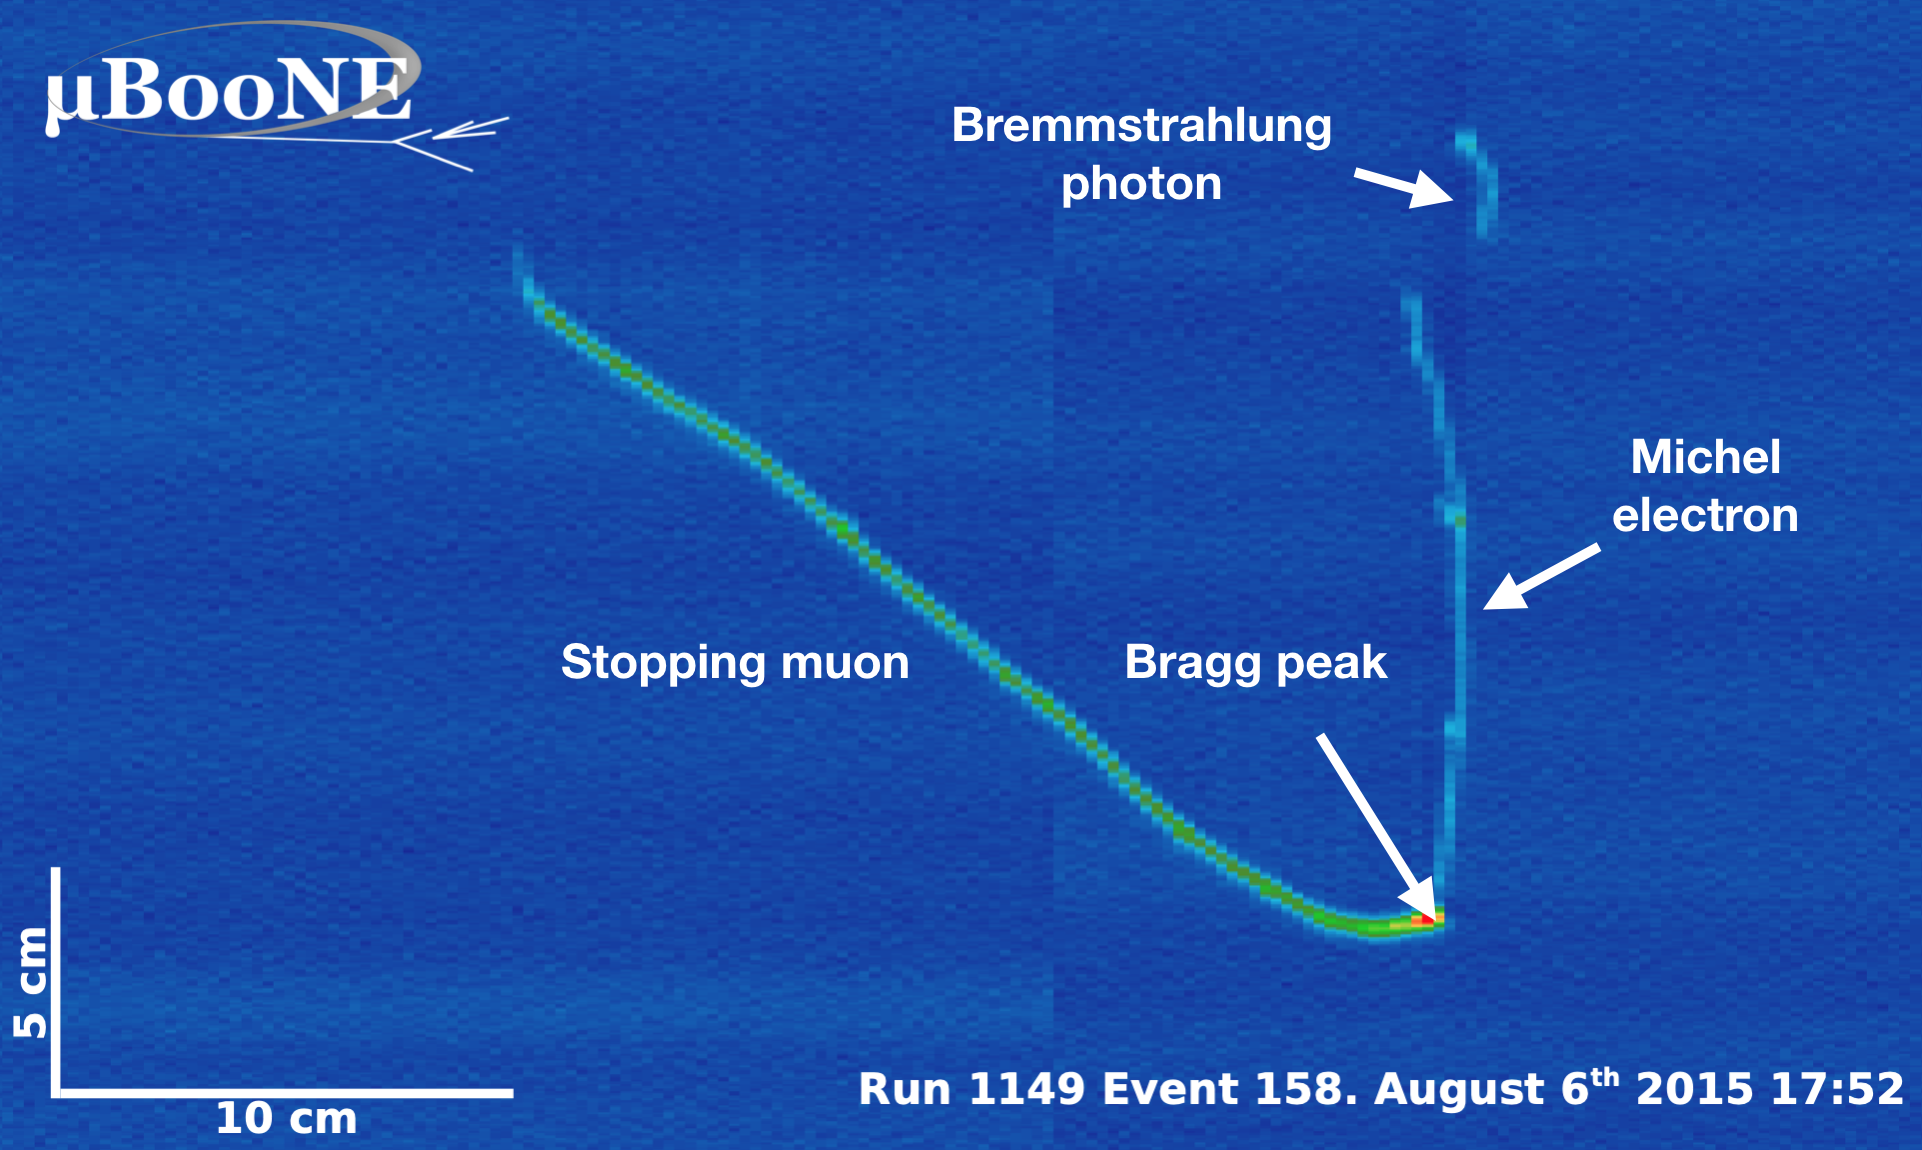
\includegraphics[width=0.75\linewidth]{figures/michel_evd.png}
  \caption{Event display of the collection plane with a muon stopping and decaying, producing a Michel electron.}
  \label{fig:michel_evd}
\end{figure}

This topology is similar to the one of an electron neutrino interaction. For this reason, stopping muons represent an important background for our analysis. 
They are tagged in two ways:
\begin{itemize}
    \item a series of pattern recognition and calorimetric algorithm try to identify the correct direction of the cosmic muon track (by measuring its energy loss profile) and to verify the presence of a \emph{kink} in the trajectory, caused by the presence of the Michel electron.
    \item the multiple Coulomb scattering (MCS) angle of a stopping muon will increase as its momentum decrease, while for through-going muons it is essentially constant \cite{Abratenko:2017nki}. By fitting the track profile with the MCS hypothesis in both direction (up-going and down-going), it is possible to verify if the cosmic muon is stopping in the detector. 
\end{itemize}

\end{description}

The hits associated with the tagged reconstructed objects (and to their daughters) are removed from the collection of reconstructed hits. The remaining hits are then fed to the Pandora \emph{neutrino mode} reconstruction path, which provides one or more neutrino interaction candidate per event. 

\subsection{Optical selection}\label{sec:optical_pre_cuts}
The optical selection serves two purposes: (1) it ensures that the optical flash which triggered the detector readout is compatible with the neutrino candidates from the Pandora neutrino mode, and (2) it provides a way to discriminate between multiple Pandora neutrino candidate objects (most of which are of cosmic origin and failed the cosmic-removal stpes) by selecting the one most compatible with the flash in the optical detection system in time with the beam-gate window.

The optical selection algorithm consists of three major stages:
\begin{enumerate}
\item cuts applied to optical properties of the reconstructed flash object (number of photoelectrons a TPC charge/PMT photoelectrons ratio);
\item cuts on the compatibility of the reconstructed flash with the Pandora neutrino candidate (position of the flash compared with the position of the centre of the collected charge);
\item the Pandora neutrino candidate which is most compatible with the flash is selected using a likelihood method.
\end{enumerate}

The effects of the optical selection have been studied in detail using the $\nu_{e}$~CC0$\pi$-Np + cosmic Monte Carlo sample, the \emph{signal}, and the data beam-off sample, the \emph{cosmic background}.

We first require a reconstructed flash in the optical system within the beam spill window of \SI{1.6}{\micro\s}. This requirement selects the 99.6\% of the signal events ($\nu_{e}$ CC0$\pi$-Np) and 18.5\% of the cosmic background events (data beam-off). 
The reconstructed flash must also have at least 50 PE recorded by the optical system. This is a very conservative requirement and keeps 99.95\% of the signal and 95.2\% of the cosmic background (Figure \ref{fig:pe_cut}).

\begin{figure}[htbp]
\centering
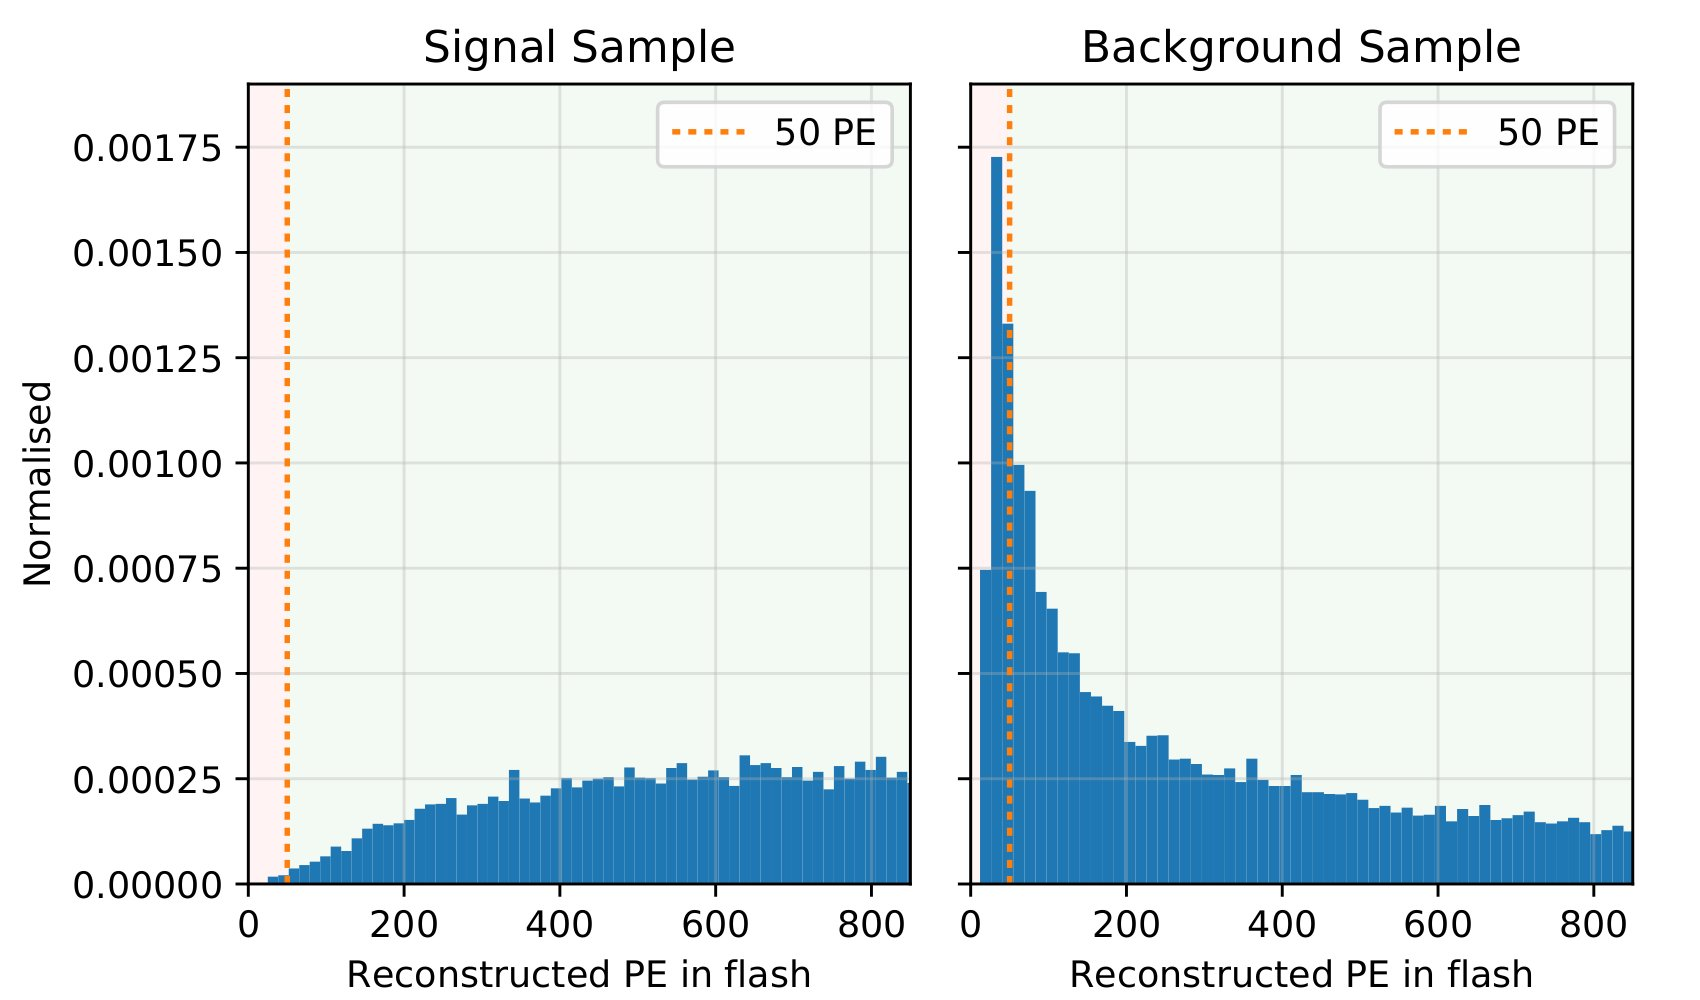
\includegraphics[width=0.85\textwidth]{figures/pe_cut.jpg} 
\caption{Reconstructed PE distribution for signal (left) and cosmic background (right) events.} 
\label{fig:pe_cut}
\end{figure}

These two cuts ensure that the event has a properly reconstructed flash. A flash object has a time and a PE count for each of the 32 PMTs. From this information, two coordinates $z\pm \sigma_z$ and $y\pm \sigma_y$ are calculated, where the positive $z$ axis corresponds to the beam direction and $y$ coordinate corresponds to the detector height. These two values can be compared with the centre of the deposited charge of the reconstructed neutrino candidate in the TPC. This comparison has the implicit assumption that the light will be emitted in the same relative fraction as the charge deposited by the particles in the final state. This is not completely correct since the amount of scintillation light produced per deposited energy unit depends on the particle. Nevertheless, the coarse resolution given by the PMT grid allows to use this approximation.

A cut of \SI{105}{\cm} is placed on the difference between the reconstructed flash position and the centre of the deposited charge on the $z$ axis. This cut keeps at least one neutrino candidate in 98.1\% of the signal events, and it removes all candidates in 20\% of the background events (Figure \ref{fig:z_cut}). 
Similar cuts are placed taking into account the width of the flash and its position on the $y$ axis. 

\begin{figure}[htbp]
\centering
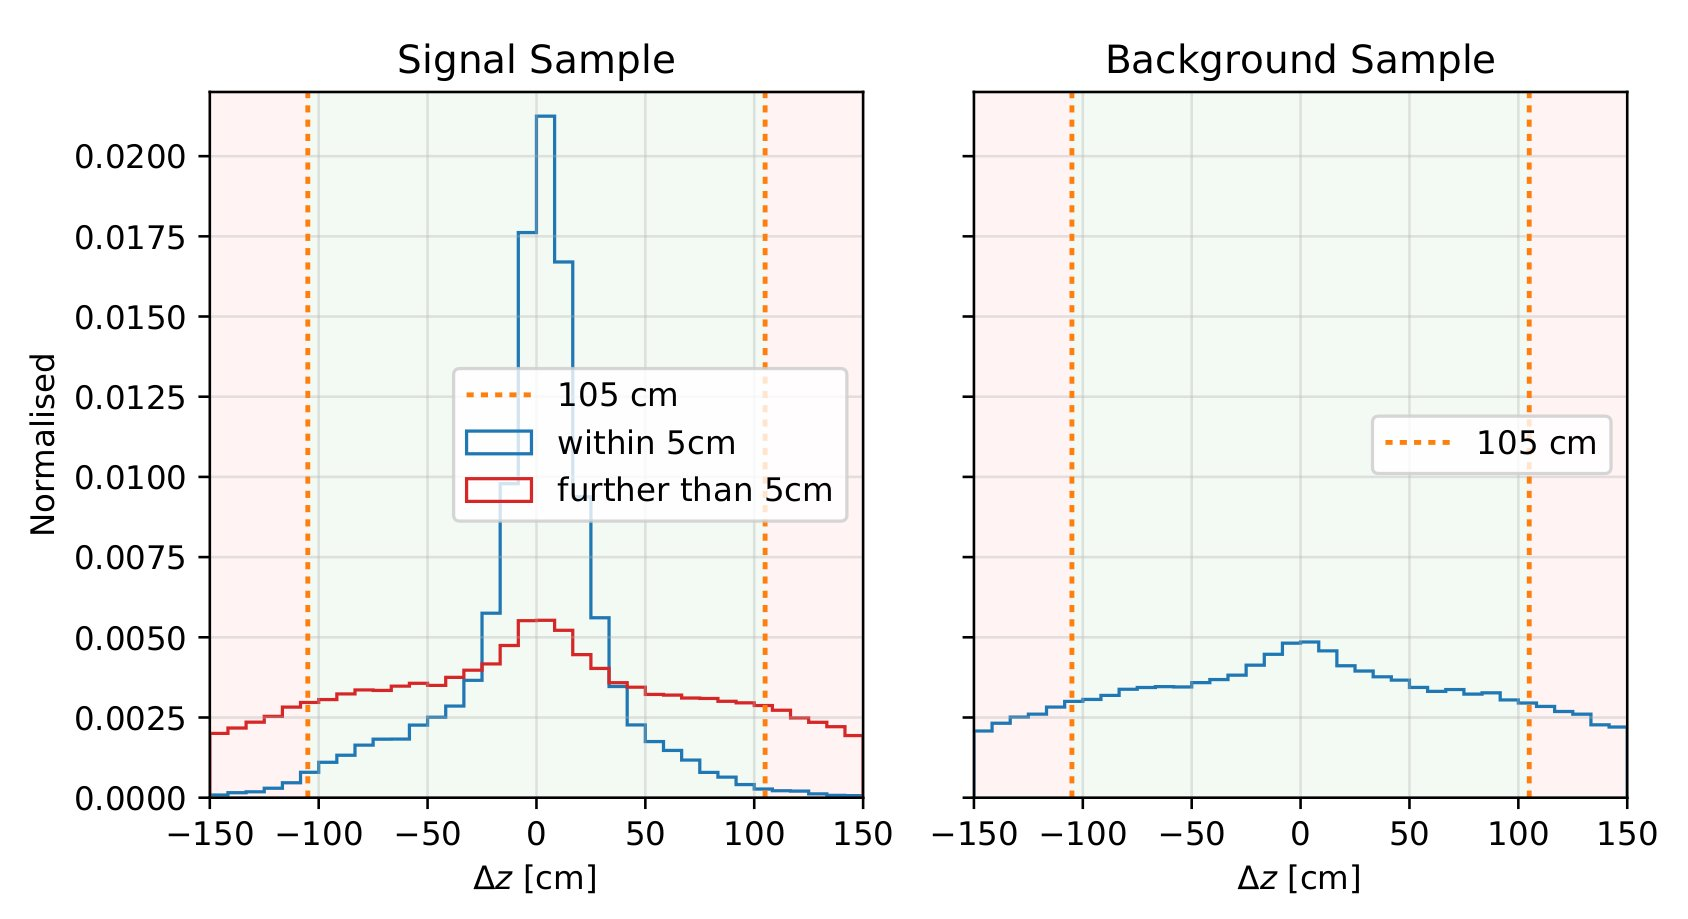
\includegraphics[width=0.85\textwidth]{figures/z_cut.jpg} 
\caption{Distribution of the distance between the reconstructed flash position and the centre of the deposited charge on the $z$ axis for signal (left) and cosmic background (right). The \emph{within 5 cm} and \emph{further than 5 cm} categories refers to the distance between the reconstructed neutrino vertex and the true neutrino vertex.} 
\label{fig:z_cut}
\end{figure}

The last rectangular cut exploits the fact that several neutrino candidates reconstructed by Pandora originate from remnants of cosmic activity which were not tagged by the cosmic-removal algorithms. Those neutrino candidates often consist in a small amount of fragmented charge, incompatible with the brightness of the flash. Placing a very conservative cut at 3.0 on the ratio between the charge in the collection plane associated to the neutrino candidate and the number of PEs reduces the signal events with a properly reconstructed flash by 1.7\%, while removing all candidates in 15.4\% of the background events (Figure \ref{fig:light_ratio}).

\begin{figure}[htbp]
\centering
\includegraphics[width=0.85\textwidth]{figures/light_ratio.jpg} 
\caption{Distribution of the ratio between the charge in the collection plane associated to the neutrino candidate (in ADC counts) and the number of PEs collected by the PMTs. The \emph{within 5 cm} and \emph{further than 5 cm} categories refers to the distance between the reconstructed neutrino vertex and the true neutrino vertex.} 
\label{fig:light_ratio}
\end{figure}

After these rectangular cuts it is still possible to have more than one reconstructed neutrino candidate in the event. A more sophisticated flash-matching procedure allows to choose the one that best matches the collected light:
\begin{enumerate}
\item for every neutrino candidate, a spatial distribution of deposited charge is measured;
\item the spatial distribution of the deposited charge is translated into an estimation of the emitted scintillation light. These scintillation photons are then propagated towards the PMTs to construct a flash hypothesis using only TPC information;
\item the flash-matching algorithm compares the reconstructed flash object as seen by the PMTs with the hypothetical flash for every reconstructed neutrino candidate and picks the best-matching candidate. This selection is achieved through a binned likelihood of the PMT spectrum.
\end{enumerate}


An example of this procedure for a Monte Carlo generated $\nu_e$ event with 4 neutrino candidates is given in Figure~\ref{fig:flashmatch}.

\begin{figure}[htbp]
\centering
\includegraphics[width=0.85\textwidth]{figures/flashmatch.png} 
\caption{An example of flash-matching. The event has 4 neutrino candidates and we make a flash hypothesis for each one, shown in red, purple, green, and brown. The observed flash corresponds to the filled blue area. A minimum binned likelihood is calculated, varying the $x$ position of the interaction. The match score is the inverse of the likelihood. The candidate with the highest match score is chosen as neutrino interaction candidate (the green one in this case).} 
\label{fig:flashmatch}
\end{figure}

\subsection{Topological pre-selection} \label{sec:topological_pre_selection}
A perfect reconstruction of a $\nu_{e}$ CC0$\pi$-Np event in a LArTPC will produce as many reconstructed tracks as the number of protons above the detection threshold in the final state and a single reconstructed shower (the electron), sharing a common vertex. However, mis-reconstruction and mis-classification issues can significantly lower the selection efficiency. The current status of the event reconstruction, which depends on the properties of the event (e.g. the number of hits \cite{Acciarri:2017hat}), affects the efficiency of selecting these events. For example, the presence of dead or unresponsive wires can affect the reconstruction by causing the splitting of an ionisation track or an electromagnetic shower into two distinct reconstructed objects. Also, the selection currently implemented relies on the classification of the reconstructed objects as track-like or shower-like, a separation that contains an inherent inefficiency, especially when the number of reconstructed hits is low.

In order to maximise our efficiency we currently require (1) \emph{at least} one track and \emph{at least} one shower sharing a common vertex, or (2) \emph{at least} two showers sharing a common vertex, to account for proton mis-classification as a shower-like object. This is because it is much more common to have protons classified as showers than electrons classified as tracks. For these cases we measure the $\chi^2$ score of the $dE/dx$ vs. residual range profile of the reconstructed objects in the proton hypothesis, as described in Section \ref{sec:proton_id}. The object with the lowest proton $\chi^2$ score is classified as a track, while the other ones remain classified as showers.

\subsection{Minimum reconstruction quality requirements}\label{sec:precuts}
A minimal set of cuts is applied to the selected events, in order to ensure that they are well reconstructed.
First, to avoid border effects, the reconstructed neutrino vertex, the start point of the reconstructed showers and the start and end points of the reconstructed tracks are required to lie within a fiducial volume. Our fiducial volume cut is 10~cm from each side on the $x$ axis, 15~cm from each side on the $y$ axis, and 10~cm (40~cm) from the upstream (downstream) side on the $z$ axis (Figure \ref{fig:fidvol}). The fiducial volume corresponds to 76.4\% of the total TPC volume. 

\begin{figure}
\centering
  \includegraphics[width=0.95\linewidth]{figures/fidvol.pdf}
  \caption{Schematic of the fiducial volume used in this analysis. The solid line corresponds to the TPC borders and the dashed red line corresponds to the fiducial volume borders.}
  \label{fig:fidvol}
\end{figure}

Since electromagnetic showers develop mainly in the forward direction with respect to the beam, the asymmetric cut on the $z$ axis (which corresponds to the beam direction) helps to reject non-fully contained events which begin too close to the downstream end of the TPC.
We also require, for each event, (1) at least 5 hits in the three planes associated to shower-like objects, (2) at least 5 hits in the three planes associated to track-like objects, and (3) at least one hit in every plane.


\subsection{Selection efficiency and purity}\label{sec:eff}
The selection efficiency of our algorithm is obtained by calculating the fraction of events selected in the $\nu_{e}$ CC$0\pi$-Np + cosmic Monte Carlo sample, where the true neutrino vertex, the start and end points of the protons, and the start point of the electron are fully contained in the fiducial volume.

In order to understand what energy thresholds are appropriate for reconstruction in the TPC, dedicated studies have been performed on proton tracks and electron showers, using the $\nu_{e}$ CC$0\pi$-Np + cosmic Monte Carlo sample, shown in Figure \ref{fig:thresholds}. We have found that we have no efficiency for reconstructing and classifying protons {with a kinetic energy} below 40~MeV and electrons{, photons, and charged pions} {with a kinetic energy} below 30~MeV following these optical, topological, and minimum quality pre-selections. Therefore, these energy thresholds are applied to the simulations to allow a fair comparison with the reconstructed particles. 

\begin{figure}
\centering
  \begin{subfigure}{0.48\textwidth}
    \includegraphics[width=\linewidth]{figures/e_efficiency.pdf}
    \caption{Electron efficiency.} 
  \end{subfigure}
    \begin{subfigure}{0.48\textwidth}
    \includegraphics[width=\linewidth]{figures/p_efficiency.pdf}
    \caption{Proton efficiency.} 
  \end{subfigure}
  \caption{$\nu_{e}$ CC$0\pi$-Np selection efficiency on single particles as a function of the true electron (left) and proton (right) kinetic energy. The dashed lines correspond to the threshold applied at truth level.}
  \label{fig:thresholds}
\end{figure}


Our overall $\nu_{e}$ CC$0\pi$-Np selection efficiency $\epsilon$ is defined as:
\begin{equation}
\epsilon = \frac{\mathrm{N.~of~selected~}\nu_{e}\mathrm{~CC0}\pi\mathrm{{\text -}Np~events}}{\mathrm{N.~of~generated~}\nu_{e}\mathrm{~CC0}\pi\mathrm{{\text -}Np~events}},
\end{equation}
where each selected event must pass the optical selection, satisfy the topology and minimum quality requirements, and not being vetoed by the independent CC $\nu_{\mu}$ selection module. %Figure \ref{fig:thresholds} shows the selection efficiency as a function of the electron and the proton kinetic energies. 



The true neutrino energy spectrum of the simulated $\nu_{e}$ CC$0\pi$-Np events in the $[0,3]$~GeV range is shown in Figure \ref{fig:true_energy}.

\begin{figure}
\centering
  \includegraphics[width=0.8\linewidth]{figures/tot.pdf}
  \caption{Simulated $\nu_{e}$ CC$0\pi$-Np true neutrino energy spectrum in the 0-3~GeV range. Each true proton (true electron) in the final state is required to have a kinetic energy larger than 40~MeV (30~MeV).}
  \label{fig:true_energy}
\end{figure}

Figure \ref{fig:effpurity} shows the efficiency as a function of the true neutrino energy.
%The energy reconstruction procedure is described in section \ref{sec:energyreco}.
The systematic uncertainties related to the cross-section and the neutrino beam flux, described in Chapter \ref{sec:systematics}, are also included. The inner error bars represent the Monte Carlo statistical uncertainty, while the outer error bars are obtained summing in quadrature the statistical and the systematic uncertainties. The statistical uncertainty $\delta\epsilon$ corresponds to the binomial error, since the application of a selection can be considered a binomial process \cite{Paterno:2004cb}:
\begin{equation}
    \delta\epsilon = \frac{1}{N}\sqrt{k(1-k/N)},
\end{equation}
where $k$ is the number of selected events and $N$ is the total number of events.

As expected, the efficiency increases with the neutrino energy, since high-energy neutrino interactions correspond in general to a larger number of hits in the TPC and the Pandora framework reconstruction performances increase with the number of reconstructed hits \cite{Acciarri:2017hat}. 

%A description of future improvements, which will allow us to increase the selection efficiency, is included in Section \ref{sec:future}.

% \todo{Add efficiency plots over a larger energy region for protons and electrons.}

\begin{figure}
\centering
%   \begin{subfigure}{0.48\textwidth}
    \includegraphics[width=0.8\linewidth]{figures/eff.pdf}
%     \caption{Efficiency.} 
%   \end{subfigure}
%     \begin{subfigure}{0.48\textwidth}
%     \includegraphics[width=\linewidth]{figures/purity.pdf}
%     \caption{Purity.} 
%   \end{subfigure}
  \caption{$\nu_{e}$ CC$0\pi$-Np selection efficiency as a function of the true $\nu_{e}$ energy. Each true proton (true electron) in the final state is required to have a kinetic energy larger than 40~MeV (30~MeV). The inner error bars represent the Monte Carlo statistical uncertainty, while the outer error bars are obtained summing in quadrature the statistical and the systematic uncertainties.}
  \label{fig:effpurity}
\end{figure}

\subsubsection{Inefficiencies breakdown}\label{sec:ineff}
Our current selection algorithm can fail for several reasons: in particular, we could have problems in the classification, such as an electron classified as a track-like object, or particles not reconstructed at all. We identified eight main causes for our selection inefficiency, whose contributions have been estimated with the same simulated sample described in Section \ref{sec:eff}. The different contributions can be visualised in Figure \ref{fig:ineff} and are described below.
\begin{description}

\item[Quality cuts (8.5\%).] The selected neutrino candidate does not satisfy our minimum quality requirements, such as the number of shower hits and the number of track hits (Section \ref{sec:precuts}).
\item[CC $\nu_{\mu}$ selected (4.3\%).] The event is tagged as a CC $\nu_{\mu}$ candidate by an independent selection module, described in \cite{ubxsec}. 
\item[Not contained (10.1\%).] One of the reconstructed tracks or the starting point of one of the reconstructed showers is not contained in the fiducial volume. As expected, this fraction increases with the neutrino energy.
\item[Cosmic selected (7.9\%).] The selected neutrino candidate has one or more reconstructed objects of cosmic origin.
\item[1 shower (3.5\%).] The selected neutrino candidate has only one associated reconstructed shower and no track object. 
\item[No showers (13.7\%).]  The selected neutrino candidate has only reconstructed track(s) associated. This is the largest contribution to the inefficiency, especially at low energies, since low-energy electrons are very challenging to reconstruct and classify as showers.
\item[No flash (5.7\%).]  The flash collected by the optical system does not satisfy our requirements, such as the minimum number of PE, location of the flash and flash hypothesis (Section \ref{sec:optical_pre_cuts}).
\item[No data products (0.7\%).] The Pandora pattern recognition did not identify any neutrion candidate.
\end{description}

Figure \ref{fig:ineff} shows a stacked histogram of the true neutrino energy for the $\nu_e$~CC0$\pi$-Np generated events, divided into the categories described above. The events without a reconstructed shower are the dominant inefficiency at low energy. Low-energy showers correspond in general to a smaller number of reconstructed hits, which makes the pattern recognition more challenging \cite{Acciarri:2017hat}. The fraction of events where at least one reconstructed object is not contained in the detector (\emph{not contained} in the legend) increases with the energy. This is expected, since the probability to have large electromagnetic showers split in two or more object increases, and these objects can have a vertex reconstructed outside the fiducial volume. The \emph{passed} category (filled grey histogram) corresponds to the efficiency plot shown in Figure \ref{fig:effpurity}.

\begin{figure}
\centering
  \includegraphics[width=0.8\linewidth]{figures/ineff_ene.pdf}
  \caption{Stacked histogram of generated events as a function of the true neutrino energy, categorised into correctly identified signal events in grey {(\emph{passed})} and different reconstruction or identification failure modes in colour.}
  \label{fig:ineff}
\end{figure}

For more detailed information, the selection outcomes as a function of the lepton true angular variables $\theta$ and $\phi$ are shown in Figure \ref{fig:ineff_angles}. The efficiency is mostly constant as a function of the azimuthal angle $\phi$, while the fraction of events without reconstructed showers increases as a function of the $\theta$ angle. This is because backwards-going electrons are more difficult to reconstruct, since they often have lower energy, and the pattern recognition tends to group the electron hits together with the forward-going proton track.

\begin{figure}
\centering
  \begin{subfigure}{0.48\textwidth}
    \includegraphics[width=\linewidth]{figures/ineff_theta.pdf}
    \caption{$\theta$ efficiency.} 
  \end{subfigure}
    \begin{subfigure}{0.48\textwidth}
    \includegraphics[width=\linewidth]{figures/ineff_phi.pdf}
    \caption{$\phi$ efficiency.} 
  \end{subfigure}
  \caption{Stacked histogram of generated events as a function of the electron $\theta$ (left) and $\phi$ (right) angles, categorised into correctly identified signal events {(\emph{passed})} in grey and different reconstruction or identification failure modes in colour.}
  \label{fig:ineff_angles}
\end{figure}

\subsection{Selection performances in BNB events}\label{sec:numu}
The previous selection efficiency results were performed on a dedicated $\nu_{e}$ CC0$\pi$-Np + cosmic sample. We now look at the selection performances when analysing events coming from the complete set of the events acquired by MicroBooNE from the Booster Neutrino Beam, including all flavours of neutrinos with different fraction (see Figure \ref{fig:bnbflux}). In the \emph{BNB+cosmic} sample every event will have at least one neutrino interacting in the cryostat volume and triggering the detector, plus all the cosmic rays hitting the detector in the same readout window. In the data, however, this is not always true, since the detector can be triggered also by a cosmic ray producing a flash in the optical system during the beam window, without necessarily having a neutrino interaction. In order to estimate this background component, defined as \emph{in-time cosmic rays}, we have used the data sample collected with the \emph{data EXT} trigger.
The background caused by the neutrino interactions happening outside the cryostat has been evaluated using the \emph{dirt} sample.
We divide the selected events (signal and background) into 8 categories:
\paragraph{Signal}
\begin{description}[labelindent=1cm]
\item[Beam intrinsic $\nu_{e}$ CC$0\pi$-Np:] charged-current $\nu_{e}$ neutrino interaction, at least one proton (N > 1), one electron, and no other visible particles above detection threshold. This category represents the signal of our analysis.
\end{description}
\paragraph{Backgrounds}
\begin{description}[labelindent=1cm]
\item[Beam intrinsic $\nu_{e}$ CC:] charged-current $\nu_{e}$ neutrino interaction that is not $\nu_{e}$ CC$0\pi$-Np or where the electron or protons were below the detection threshold defined above.
\item[Beam intrinsic $\nu_{\mu}$:] charged-current $\nu_{\mu}$ neutrino interaction.
\item[Beam intrinsic NC:] neutral current neutrino interaction (both $\nu_{\mu}$ and $\nu_{e}$).
\item[Outside fiducial volume:] neutrino interaction which occurs outside the fiducial volume, but with one or more final-state particles inside in the fiducial volume.
\item[Cosmic contaminated:] neutrino interaction candidate with at least a cosmogenic track or shower, attached to a correctly reconstructed neutrino candidate.
\item[Cosmic:] cosmic ray interaction happening in the same readout window is mistakenly chosen instead of the neutrino interaction in the event. 
\item[Data beam-off]: event with no neutrino interaction, but where a cosmic-ray interaction in time-coincidence with the beam-gate window triggered the event, and activity was selected as a neutrino candidate.
\end{description}

Table \ref{tab:result} shows a summary of the selection algorithm results, with the corresponding number of events for each category.
%The numbers correspond to an exposure of the MicroBooNE detector of \num{4.34e19} protons on target (POT). This is equivalent to the amount of data analysed here, which is a subset of the data collected from February to April 2016.

\begin{table}[htbp]
   \centering
      \caption{Summary of the selection results, showing the contribution of each event category, for a MicroBooNE exposure of \num{4.34e19} POT. Efficiency uncertainties are statistical only. {For the \emph{Cosmic contaminated} category the number of generated events correspond to the number of neutrino interactions inside the cryostat. For the \emph{Cosmic} category, it corresponds to the total number of simulated neutrino interactions, both inside and outside the cryostat.}}\label{tab:result}
   \begin{tabular}{lrrr}
     \toprule
     Category & Generated & Selected & Efficiency [\%]\\
     \midrule

     \textbf{$\nu_{e}$ CC0$\pi$-Np (signal)}  & $33.8$    & $15.4$  & $45.5\pm0.5$\\
     $\nu_{e}$ CC                             & $39.5$    & $15.4$  & $39.0\pm0.5$\\
     Beam intrinsic $\nu_{\mu}$               & $10905.9$ & $488.9$ & $4.5\pm0.2$\\
     Beam intrinsic NC                        & $3532.8$  & $329.5$ & $9.3\pm0.2$\\
     Outside fid. vol.                        & $36634.6$ & $79.0$  & $0.2\pm0.1$\\
     Data off-beam                            & $123070.2$ & $1593.4$ & $1.3\pm0.1$\\
     Cosmic contaminated                      & $14706.4$  & $376.1$  & $2.5\pm0.1$\\ 
     Cosmic                                   & $51356.1$  & $489.4$  & $0.8\pm0.1$\\

     \bottomrule
   \end{tabular}

\end{table}

At this point, all selected events have a neutrino interaction candidate with one or more tracks and one or more showers associated with the interaction vertex. Since we use two different methods to measure the energy of the tracks and the energy of the showers (see Section \ref{sec:energyreco}), it is necessary to verify the agreement between the shower multiplicity and track multiplicity distributions in data and Monte Carlo. Figure \ref{fig:multiplicity} shows that the two distributions agree within the systematic uncertainties, whose evaluation is described in Section \ref{sec:systematics}.

\begin{figure}[htbp]
\centering
  \begin{subfigure}{0.49\textwidth}
    \includegraphics[width=\linewidth]{figures/n_tracks.pdf}
    \caption{Track multiplicity.} 
  \end{subfigure}\hfill
    \begin{subfigure}{0.49\textwidth}
    \includegraphics[width=\linewidth]{figures/n_showers.pdf}
    \caption{Shower multiplicity.} 
  \end{subfigure}
  \caption{Distributions of the track and shower multiplicities in data and Monte Carlo simulation.}\label{fig:multiplicity}
\end{figure}

The agreement between data and simulation is also verified in the angular distributions of the reconstructed showers objects, shown in Figure \ref{fig:thetaphi}. As expected, the neutrino distributions are mostly constant as a function of the azimuthal angle $\phi$ and peaked at low inclination angle $\theta$ values, since the interactions are mostly forward going. The inclination angle $\theta$ distribution agrees within the uncertainties both for shape and normalisation. The azimuthal angle $\phi$ distribution shows a slight disagreement around $\phi = 0^{\circ}$ and $\phi = \pm180^{\circ}$. This is caused by an imprecise signal simulation that predominantly affects tracks moving exactly towards or away from the anode \cite{Adams:2018gbi}. This effect is taken into account in the Dynamic Induced Charge detector systematic sample (Section \ref{sec:systematics}). 

Figure \ref{fig:thetaphi_pdg} shows the angular distributions classified according to the primary particle that generated the shower (in the case of a Michel electron the shower is placed in the muon category). Each entry in the histogram correspond to a reconstructed shower, so it is possible to have more than one entry per event. As expected, the $\theta$ distribution is peaked at low angles, since neutrino interactions are mostly forward going. The $\phi$ distribution is mainly flat for neutrino-induced particles (electrons, photons) and with two peaks at $\pm90^{\circ}$ for mostly-vertical cosmic-induced particles (mainly muons). In this case, the data points correspond to the bin-by-bin statistical subtraction of the beam-on and beam-off entries.

\begin{figure}[htbp]
\centering
  \begin{subfigure}{0.49\textwidth}
    \includegraphics[width=\linewidth]{figures/h_shower_theta.pdf}
    \caption{Inclination angle $\theta$.} 
  \end{subfigure}\hfill
    \begin{subfigure}{0.49\textwidth}
    \includegraphics[width=\linewidth]{figures/h_shower_phi.pdf}
    \caption{Azimuth angle $\phi$.} 
  \end{subfigure}
  \caption{Distributions of the inclination angle $\theta$ and the azimuthal angle $\phi$ of the reconstructed showers in the selected events for each event category. The black points represent the data with statistical uncertainties. The coloured stacked histograms represent the simulated events, with the hatched histogram corresponding to the data beam-off sample. The shaded area represents the systematic uncertainty. The bottom part of the plot shows the ratio between the data beam-on events and the stacked histograms.}\label{fig:thetaphi}
\end{figure}

\begin{figure}[htbp]
\centering
  \begin{subfigure}{0.49\textwidth}
    \includegraphics[width=\linewidth]{figures/h_shower_theta_pdg.pdf}
    \caption{Inclination angle $\theta$.}\hfill
  \end{subfigure}
    \begin{subfigure}{0.49\textwidth}
    \includegraphics[width=\linewidth]{figures/h_shower_phi_pdg.pdf}
    \caption{Azimuth angle $\phi$.} 
  \end{subfigure}
  \caption{Distributions of the inclination angle $\theta$ and the azimuthal angle $\phi$ of the reconstructed showers, classified according to the primary particle that generated them. The black points represent the statistically subtraction of the data beam-off events from the data beam-on events. The coloured stacked histograms represent the simulated events. The shaded area represents the systematic uncertainty. The bottom part of the plot shows the ratio between the statistical subtraction and the stacked histograms.}\label{fig:thetaphi_pdg}
\end{figure}

A small fraction of the data events was also visually inspected: Figure \ref{fig:evds} shows three event displays of data events compatible with a $\nu_{e}$ CC0$\pi$-Np interaction. 

\begin{figure}[htbp]
\centering
  \begin{subfigure}{0.45\textwidth}
  \includegraphics[width=\linewidth]{figures/data3.png}
    \caption{Event 1515, Subrun 30, Run 5328}\end{subfigure}
  \hfill\begin{subfigure}{0.45\textwidth}	
  \includegraphics[width=\linewidth]{figures/data2.png}
  \caption{Event 31, Subrun 0, Run 5513}
\end{subfigure}
\vspace{1em}

  \begin{subfigure}{0.45\textwidth}	
  \includegraphics[width=\linewidth]{figures/data1.png}
  \caption{Event 3710, Subrun 74, Run 5906}
\end{subfigure}

  \caption{Event displays of the collection plane of three $\nu_{e}$-like data events selected by our algorithm. The gaps are caused by the presence of missing wires. The red lines correspond to reconstructed track-like objects and the green cones correspond to reconstructed shower-like objects. }
  \label{fig:evds}
\end{figure}


\section{Calorimetry}\label{sec:energyreco}
\subsection{Scope of the energy reconstruction}
In this analysis we restrict ourselves to the measurement of the deposited energy in the TPC of the visible particles in the final state of the $\nu_e$ CC0$\pi$-Np neutrino interaction. Our signal has in its final state, by definition, one electron and at least one proton, with no other visible particles. The energy of the electron is measured by converting the reconstructed charge of all the shower-like objects into deposited energy, as described in Section \ref{sec:showerenergy}. The energy of the protons, instead, can be measured by converting the track length of the reconstructed tracks into deposited energy, using the tabulated stopping power of protons in the liquid argon, with the procedure described in \ref{sec:protonenergy}. The total reconstructed energy corresponds to the sum of the reconstructed energies, corrected by the calibration factors calculated below, and is referred to as $E_{\mathrm{corr}}$. This quantity is then compared with the total kinetic energy of the particles above detection thresholds and corrected by a calibration factor to obtain an estimate of the deposited energy $E_{\mathrm{deposited}}$ (Section \ref{sec:deposited}).


\subsection{Electron energy reconstruction and calibration}\label{sec:showerenergy}
The reconstructed energy $E_{\mathrm{reco}}^{e}$ of a shower-like object is measured converting the charge of the associated hits into deposited energy in the TPC. It is calculated by multiplying the reconstructed charge ($e^{-}_{\mathrm{reco}}$) from hits associated with the reconstructed shower by the calibration factor \cite{Acciarri:2017sjy}:
\begin{equation}
\frac{E_{\mathrm{reco}}^{e} \mathrm{(MeV)}}{e^{-}_{\mathrm{reco}}} = 1.01\frac{e^-}{e^{-}_{\mathrm{reco}}} \times \frac{23.6~\mathrm{eV}}{e^-} \times 10^{-6} \frac{\mathrm{MeV}}{\mathrm{eV}} \times \frac{1}{R} = 3.85\times10^{-5},\label{eq:calib}
\end{equation}
where:
\begin{itemize}

\item the correction factor $1.01\frac{e^-}{e^{-}_{\mathrm{reco}}}$ is obtained measuring the true number of collected electrons $e^{-}$ on the wires using a sample of stopping muons, fitting the $dE/dx$ vs. residual range to values for argon as tabulated by the PDG \cite{PhysRevD.98.030001};
\item $\frac{23.6~\mathrm{eV}}{e^-}$ is the work function for ionizing an argon atom \cite{Shibamura:1975zz};
\item $R = 0.62$ is the recombination factor obtained with the Modified Box Model \cite{Acciarri:2013met} at MicroBooNE's electric field of 270~V/cm assuming an energy loss per length $dE/dx=2.3$~MeV/cm.
\end{itemize}

The reconstructed energy is obtained summing the energy of each hit from the reconstructed showers produced by a simulated electron in the collection plane, produced by a $\nu_{e}$ CC0$\pi$-Np interaction. The starting point of the simulated electron and the starting point of the reconstructed showers are required to be within the fiducial volume. 
Figure \ref{fig:ecalib} shows the calibration slope necessary to convert the electron reconstructed energy $E_{\mathrm{reco}}^{e}$ into true electron energy $E^{e}$. The true energy spectrum has been divided into 10 bins of equal size in the 30-2030~MeV range. Since the reconstructed energy distributions in each true energy bin are asymmetric, the data points are obtained fitting the distributions with a GaussExp function \cite{Das:2016stf}, in order to estimate the most probable value (MPV). The GaussExp function consists of an exponential tail stitched to a Gaussian core and it is often use to measure lossy processes such as the energy reconstructed in a calorimeter. The coordinate on the $E^{e}$ axis are given by the mean of the true energy distribution for each bin. The vertical error bars correspond to the full width at half maximum (FWHM) of the fitted function. The true energy distribution and the reconstruction energy distribution for every bin are shown in Figure \ref{fig:e_spectra}.

\begin{figure}[htbp]
\centering
\begin{overpic}[width=0.95\linewidth]{figures/e_spectra.pdf}
\end{overpic}
% \includegraphics[width=0.65\columnwidth]{figures/ecalib.pdf}
\caption{Reconstructed and true energy distribution for 10 intervals of equal size in the 30-2030 MeV energy range. The reconstructed energy distribution have been fitted with a GaussExp function.}
\label{fig:e_spectra}
\end{figure}


The linear fit of the most probable value points, shown in Figure \ref{fig:ecalib} gives:
\begin{equation}
E_{\mathrm{reco}}^{e} = 0.77~E^{e} - 34.7~\mathrm{MeV}.
\end{equation}
The energy of the shower, corrected by the calibration factor is then defined as:
\begin{equation}
E_{\mathrm{corr}}^{e} = (E_{\mathrm{reco}}^{e} + 34.7~\mathrm{MeV})/0.77.
\end{equation}

\begin{figure}[htbp]
\centering
\begin{overpic}[width=0.7\linewidth]{figures/ecalib.pdf}
\end{overpic}
% \includegraphics[width=0.65\columnwidth]{figures/ecalib.pdf}
\caption{Bi-dimensional histogram of true electron energy $E^{e}$ vs. reconstructed electron energy $E_{\mathrm{reco}}^{e}$. The reconstructed electron energy is measured summing the energy of each hit associated to reconstructed showers produced by the simulated electron. The black points correspond to the most probable value of the $E_{\mathrm{reco}}^{e}$ distribution for each $E^{e}$ bin, calculated with a GaussExp fit.}
\label{fig:ecalib}
\end{figure}

It is also possible to measure the energy resolution in the simulation by calculating the normalised difference $E_{\mathrm{frac}}$ between the corrected reconstructed energy $E^e_{\mathrm{corr}}$ and the true electron energy $E^e$:
\begin{equation}
    E_{\mathrm{frac}} = \frac{E^e_{\mathrm{corr}}-E^e}{E^e}.
\end{equation}
Figure \ref{fig:electron_res} shows the $E_{\mathrm{frac}}$ distribution for 10 intervals of equal size between 30 and 2030~MeV and the GaussExp fit for each distribution.

\begin{figure}[htbp]
\centering
\begin{overpic}[width=0.95\linewidth]{figures/electron_res.pdf}
\end{overpic}
% \includegraphics[width=0.65\columnwidth]{figures/ecalib.pdf}
\caption{Normalised energy difference $E_{\mathrm{frac}}$ for 10 intervals of equal size in the 30-2030 MeV energy range. The normalised energy difference distributions have been fitted with a GaussExp function (red line).}
\label{fig:electron_res}
\end{figure}

The fractional energy resolution can then be defined as the ratio between the standard deviation of the Gaussian core $\sigma$ of the GaussExp function and the true electron energy $E_e$. Figure \ref{fig:sigma_e} shows the fractional energy resolution as a function of the true electron energy. The points can be fitted with the classic calorimeter resolution formula \cite{Fabjan:2003aq}:
\begin{equation}
    \frac{\sigma}{E} = \frac{a}{\sqrt{E}} \oplus \frac{b}{E} \oplus c,\label{eq:calo}
\end{equation}
where:
\begin{itemize}
    \item $a = 2.30\%$ is the stochastic term, which is caused by the intrinsic fluctuations of the development of the electromagnetic shower;
    \item $b = 7.53\%$ is the noise term, which comes from the electronics noise of the readout chain and represents the dominant contribution;
    \item $c = 1.21\%$ is the constant term, which is caused by detector non-uniformities (e.g. the presence of missing or unresponsive wires).
\end{itemize} 

\begin{figure}[htbp]
\centering
\begin{overpic}[width=0.85\linewidth]{figures/sigma_e.pdf}
\end{overpic}
\caption{Fractional energy resolution for 10 intervals of equal size in the 30-2030 MeV energy range. The points have been fitted the classic calorimeter energy resolution formula \eqref{eq:calo}.}
\label{fig:sigma_e}
\end{figure}


Another effect which contributes to the broadening of the energy resolution in MicroBooNE is caused by wrong or sub-optimal clustering: if the pattern recognition fails to group together all the hits that corresponds to the electromagnetic shower, or if it includes hits belonging to ionisation tracks (e.g. from cosmic muons), the reconstructed energy will be respectively smaller or larger than the true electron energy.
It is also important to underline that the energy resolution quoted here does not correspond to the intrinsic MicroBooNE energy resolution, but only to the energy resolution for the selected $\nu_e$ CC0$\pi$-Np events.

\subsection{Single proton energy reconstruction and calibration}\label{sec:protonenergy}
Proton energy reconstruction is performed by converting the reconstructed track length $L$ into deposited energy using the proton stopping power in liquid argon tabulated in \cite{pstar}. Liquid argon density $\rho_{\mathrm{LAr}}$ is assumed to be constant at 1.4~g/ml. Figure \ref{fig:proton} shows the proton kinetic energy as a function of the range of the proton in liquid argon (measured as $L \times \rho_{\mathrm{LAr}}$).

\begin{figure}[htbp]
\centering
  \begin{subfigure}{0.49\textwidth}
  \begin{overpic}[width=\linewidth]{figures/proton.pdf}
\put(120,640){\tiny{\textsf{\textbf{MicroBooNE Simulation Preliminary}}}}
\end{overpic}
%     \includegraphics[width=\linewidth]{figures/proton.pdf}
    \caption{Proton kinetic energy as a function of the range of the proton in liquid argon.}\label{fig:proton}
  \end{subfigure}
  \begin{subfigure}{0.49\textwidth}
    \begin{overpic}[width=\linewidth]{figures/pcalib.pdf}\end{overpic}
% 	\includegraphics[width=\linewidth]{figures/pcalib.pdf}
     \caption{Bi-dimensional histogram of true proton energy $E^{p}$ vs. reconstructed proton energy $E_{\mathrm{reco}}^{p}$.}\label{fig:pcalib}
   \end{subfigure}
   \caption{The reconstructed proton energy is measured converting the reconstructed track length $L$ into deposited energy using the proton stopping power in liquid argon, as tabulated in \cite{pstar} (left). The calibration is calculated from a linear fit of the most probable values of the $E_{\mathrm{reco}}^{p}$ distribution for each $E^{p}$ bin (right).}
\end{figure}

The calibration constant has been obtained comparing the reconstructed energy of the proton with the true kinetic energy of the simulated proton, in a CC $\nu_{e}$ sample with only one proton in the final state. The true proton and the reconstructed tracks are required to be fully contained within the fiducial volume. Since protons are not minimum-ionising particles, in the case of two or more tracks (\emph{split tracks}) associated to the same proton, the reconstructed length of the tracks has been summed before calculating the corresponding kinetic energy.
Figure \ref{fig:pcalib} shows the calibration slope necessary to convert the proton reconstructed energy $E_{\mathrm{reco}}^{p}$ into true proton kinetic energy $E^{p}$. For each bin of the true proton energy, the most probable value of the corresponding proton reconstructed energy has been obtained with a GaussExp fit. A linear fit of the most probable values gives:
\begin{equation}
E_{\mathrm{reco}}^{p} = 1.00~E^{p} - 2.9~\mathrm{MeV}.
\end{equation}
The energy of the track, corrected by the calibration factor is then defined as:
\begin{equation}
E_{\mathrm{corr}}^{p} = (E_{\mathrm{reco}}^{p} + 2.9~\mathrm{MeV})/1.00
\end{equation}

\subsection{Deposited Energy Reconstruction}\label{sec:deposited}
It is possible to compare the total visible energy in the event $E_{\mathrm{k}}$, defined as the sum of the kinetic energies of the visible particles in the final state, with the sum of the reconstructed energies for shower-like ($E_{\mathrm{corr}}^{e}$) and track-like objects ($E_{\mathrm{corr}}^{p}$) for the selected $\nu_{e}$ CC0$\pi$-Np events. This quantity $E_{\mathrm{corr}}$ is defined as:
\begin{equation}
E_{\mathrm{corr}} = \sum^{N_{p}} E_{\mathrm{corr}}^{p} + \sum^{N_{e}} E_{\mathrm{corr}}^{e},
\end{equation}
where $N_{p}$ is the number of reconstructed tracks and $N_{e}$ is the number of reconstructed showers in the event. For events where we have two or more shower-like objects and no track-like objects, the shower-like object with the lowest proton $\chi^2$ score is chosen as proton candidate (see Section \ref{sec:proton_id}). In these cases we have $N_{p} = 1$ by definition.
The reconstructed energy does not include particles that do not interact in the liquid argon (such as neutrons) and charged particles with a kinetic energy below the detection threshold, defined in Section \ref{sec:eff}. Figure \ref{fig:nucalib} shows the calibration slope necessary to convert the the total reconstructed energy $E_{\mathrm{corr}}$ into visible energy $E_{\mathrm{k}}$. The plot has been obtained using the $\nu_{e}$ CC0$\pi$-Np + cosmic sample. A linear fit of the data points gives:
\begin{equation}
E_{\mathrm{k}} = 0.98~E_{\mathrm{corr}} - 28.5~\mathrm{MeV}.
\end{equation}
The reconstructed visible energy, corrected by the calibration factor is then defined as:
\begin{equation}
E_{\mathrm{deposited}} = (E_{\mathrm{corr}} + 28.5~\mathrm{MeV})/0.98
\end{equation}

Several effects can contribute to this calibration factor: among the others, the presence of regions with unresponsive of missing wires can cause an underestimation of the deposited energy. In the future, this effect can be limited by the use of the other two planes for calorimetric measurements.

\begin{figure}[htbp]
\centering
\begin{overpic}[width=0.85\linewidth]{figures/nucalib.pdf}
\end{overpic}\caption{Bi-dimensional histogram of total visible energy $E^{\mathrm{k}}$ vs. the total reconstructed energy $E_{\mathrm{corr}}$. Black points are obtained measuring the most probable value of the $E_{\mathrm{corr}}$ distribution for each $E_{\mathrm{k}}$ bin.} 
\label{fig:nucalib}
\end{figure}

In this analysis, we will use the quantity $E_{\mathrm{deposited}}$ as an estimate of the total visible energy in the event.

\subsection{Deposited energy binning}\label{sec:depositedenergy}
The binning of the deposited energy distribution must be carefully evaluated, since it is of fundamental importance in the calculation of the significance of an eventual excess. In this analysis, we require the events in a true $E_{\mathrm{k}}$ bin to fall in the same reconstructed $E_{\mathrm{deposited}}$ bin in at least 50\% of the cases for $\nu_e$~CC0$\pi$-Np events. A combination which satisfies this condition and maximises the number of bins in the $[0,3]$~GeV range is:
\begin{equation}
    E_{\mathrm{deposited}}\text{~bins} = [0, 0.2, 0.4, 0.6, 0.9, 1.25, 1.9, 3]~\text{GeV},
\end{equation}
which is then chosen as our binning for the $E_{\mathrm{deposited}}$ distributions.
Figure \ref{fig:migration} shows the migration matrix between $E_{\mathrm{deposited}}$ and $E_{\mathrm{k}}$. It shows the probability that an event with a true energy $E_{\mathrm{k}}$ in the $i$ bin has a reconstructed energy $E_{\mathrm{deposited}}$ in the same $i$ bin. Our binning criteria ensures that each element on the diagonal has a value larger than 0.50.

\begin{figure}[htbp]
\centering
\begin{overpic}[width=0.85\linewidth]{figures/migration.pdf}
\end{overpic}
\caption{Migration matrix between $E_{\mathrm{deposited}}$ and $E_{\mathrm{k}}$. It shows the probability that an event with a true energy $E_{\mathrm{k}}$ in the $i$ bin has a reconstructed energy $E_{\mathrm{deposited}}$ in the same $i$ bin.}
\label{fig:migration}
\end{figure}


\subsection{Measurement of the electromagnetic shower energy loss}\label{sec:dedx}
The mean energy loss per length of charged particles $\left\langle dE/dx\right\rangle$ can be described by the \emph{Bethe equation} as defined in Section 30.2.2 of \cite{PhysRevD.98.030001}:
\begin{equation}
    -\left\langle\frac{dE}{dx}\right\rangle = Kz^2\frac{Z}{A}\frac{1}{\beta^2}\left[\frac{1}{2}\ln\frac{2m_e c^2\beta^2\gamma^2 T_{\mathrm{max}}}{I^2}-\beta^2-\frac{\delta(\beta\gamma)}{2}\right],\label{eq:bethe}
\end{equation}
where $T_{\mathrm{max}}$ is the maximum possible energy transfer in a single collision, $I$ is the mean excitation energy, and $\delta(\beta\gamma)$ is a density correction. 

In materials of moderate thickness such as LAr, the energy loss probability distribution is described by the asymmetric Landau distribution \cite{Landau:1944if}, which drives the mean of the energy loss of eq. \eqref{eq:bethe} into the tail of the distribution. For this reason, ``the
mean of the energy loss given by the Bethe equation [\dots] is thus ill-defined
experimentally and is not useful for describing energy loss by single particles'' (Section 30.2.7 of \cite{PhysRevD.98.030001}).
The most probable value of the Landau distribution, which should be used instead, is given by: 
\begin{equation}
    \Delta_p = \xi\left[\ln\frac{2mc^2\beta^2\gamma^2}{I}+\ln\frac{\xi}{I}+j-\beta^2-\delta(\beta\gamma)\right],\label{eq:landau}
\end{equation}
where $\xi = (K/2)\langle Z/A \rangle (x/b^2)$~MeV, $j=0.2$, and $x$ is the thickness of the material in $\mathrm{g}\cdot\mathrm{cm}^2$ (Section 30.2.7 of \cite{PhysRevD.98.030001}). 

An important feature of the LArTPC technology is its ability to distinguish between electrons and photons in the final state by measuring their $dE/dx$. Photons that undergo pair-production, which is the dominant process above 10~MeV, produce a $e^+e^-$ pair. If the pair is boosted, the trajectories of the positron and the electron overlap, producing an average $dE/dx$ which is twice the one of a single, minimum-ionising electron. 

In MicroBooNE, the $dE/dx$ for electromagnetic showers is measured with a procedure analogous to the one developed by the ArgoNeuT collaboration and described in \cite{Acciarri:2016sli}. In this document, neutrinos were produced by the NuMI neutrino beam and the events were visually inspected to select electron and photon showers.

\begin{figure}[htbp]
\centering
\begin{overpic}[width=0.75\linewidth]{figures/evd_dedx.pdf}
\end{overpic}\caption{Event display of an electron shower candidate, showing the $1\times4$~cm$^2$ area used for the $dE/dx$ calculation. Each small black rectangle corresponds to a reconstructed shower hit.}
\label{fig:evd_dedx}
\end{figure}

In our implementation, as a first step, all the hits of the collection plane within a rectangle of 4~cm along the direction of the shower and 1~cm perpendicular to the shower are collected, as shown in the event display in Figure \ref{fig:evd_dedx}.

Subsequently, the $dQ/dx$ for each hit is measured dividing the collected charge ($dQ$) by the pitch ($dx$) between each hit and the next one along the shower direction. The pitch corresponds to the distance in the TPC that a particle travels between its two projections  on adjacent wires, which is \emph{at least} the wire spacing (3~mm for MicroBooNE \cite{Acciarri:2016smi}). Electromagnetic showers aligned with the wire direction correspond to a large value of the pitch. 

The $dE/dx$ is calculated from the $dQ/dx$ using the calibration factor measured in Section \ref{sec:showerenergy}, eq. \eqref{eq:calib}.
Since the Landau distribution of the $dE/dx$ hit values has an asymmetric tail, we assign to the shower the median (and not the mean) of the $dE/dx$ hit distribution, as an estimation the most probable value. The median metric has been proved in \cite{Acciarri:2016sli} to be to most robust over a variety of box lengths.

\begin{figure}[htbp]
\centering
\begin{overpic}[width=0.75\linewidth]{figures/dedx.pdf}
\end{overpic}\caption{Area-normalised distributions for the measured $dE/dx$ for simulated electrons and photons.}
\label{fig:dedx_gamma_e}
\end{figure}

Figure \ref{fig:dedx_gamma_e} shows the area-normalised histograms of the $dE/dx$ in the collection plane for simulated electron and photon showers. The events below 1~MeV/cm correspond for both distributions to showers with a low number of associated hits, or where the shower was mostly aligned with the wires of the collection plane (having as such a high pitch value). Figure \ref{fig:pitch} shows the pitch distribution in the collection plane and a bi-dimensional histogram of the $dE/dx$ vs. the pitch for photon showers: events with a $dE/dx$ below 1~MeV/cm mostly correspond to a high value of the pitch. 

\begin{figure}[htbp]
  \begin{subfigure}{0.49\textwidth}
  \begin{overpic}[width=0.88\linewidth]{figures/pitch.pdf}
\end{overpic}
    \caption{Pitch distribution for simulated electron showers in the collection plane (log-scale).}
  \end{subfigure}\hfill
  \begin{subfigure}{0.49\textwidth}
    \begin{overpic}[width=\linewidth]{figures/dedx_vs_pitch.pdf}\end{overpic}
     \caption{Bi-dimensional histogram of measured $dE/dx$ vs. pitch for photon showers.}
   \end{subfigure}
   \caption{Electromagnetic showers aligned with the wire orientation will have a large pitch value and their measured $dE/dx$ will be shifted towards low values.}\label{fig:pitch}
\end{figure}

The electron showers have a peak around 2~MeV/cm, as expected. The photon showers, instead, have a peak around 4~MeV/cm and a second peak around 2~MeV/cm, which represents a limitation to our $e/\gamma$ separation capabilities. This peak is caused by mainly two effects:
\begin{itemize}
    \item photons that undergo Compton scattering will transfer most of their energy to the electron, producing a shower with the same $dE/dx$ of an electron. This effect decreases with the photon energy and is dominant below 10~MeV, as shown in Figure \ref{fig:compton};
    
    \begin{figure}[htbp]
    \centering
    \begin{overpic}[width=0.75\linewidth]{figures/compton.png}
    \end{overpic}\caption{Cross section of gammas on argon between 1 MeV and 1 GeV. Here, $\kappa$ refers to the pair production cross section for the nuclear field and electron field. Compton scattering is dominant below 10 MeV. From \cite{Acciarri:2016sli}.}
    \label{fig:compton}
    \end{figure}
    
    \item very asymmetric $\gamma\rightarrow e^+e^-$ pair production. When the positron and the electron do not overlap, the measured $dE/dx$ distribution will be peaked around 2~MeV/cm. The electron and the positron can also be produced with very different energies, as shown in Figure \ref{fig:asymmetry}. In this case, the distribution of the $dE/dx$ values in the $1\times4$~cm$^2$ box will be shifted towards 2~MeV/cm. 
    
    \begin{figure}[htbp]
    \centering
    \begin{overpic}[width=0.75\linewidth]{figures/asymmetry.pdf}
    \end{overpic}\caption{Pair production relative cross-section as a function of the fraction of the photon energy $k$ transferred to either the electron or positron with energy $\epsilon$. From \cite{Caratelli:2018nob}.}
    \label{fig:asymmetry}
    \end{figure}
\end{itemize}

A comparison between the data and Monte Carlo distributions of the reconstructed showers $dE/dx$ is shown in Figure \ref{fig:dedx_datamc} of Section \ref{sec:bkg}.

\subsection{Particle identification of reconstructed tracks}\label{sec:proton_id}
The measurement of the $dE/dx$ along the reconstructed tracks allows to perform powerful particle identification, as demonstrated by a the ArgoNeuT collaboration in \cite{Acciarri:2013met}. 

This capability is particularly important for the search of low-energy electron neutrinos. A $\nu_e$ CC0$\pi$-1p neutrino interaction is topologically identical to a cosmic muon stopping in the LAr, since they both appear as a track with a small shower attached. However, the energy loss of a proton produced in a neutrino interaction is sensibly different from the one of a cosmic muon, for two main reasons:
\begin{itemize}
    \item the Bragg peak of the stopping cosmic muon corresponds to starting point of the Michel electron shower, while the Bragg peak of the proton track is far from the interaction vertex;
    \item the proton $dE/dx$ profile for protons differs from the $dE/dx$ profile for muons.
\end{itemize}
Being able to distinguish between proton and muon tracks is therefore essential in order to reject cosmogenic background. Events with a $\nu_{\mu}$ interaction with only a stopping muon in the final state can also be rejected with the same technique.

It is possible to parametrise the relation between the theoretical $dE/dx$ of a ionisation track and its \emph{residual range} with a power-law function:
\begin{equation}
    \frac{dE}{dx} = A R^b,
\end{equation}
where $A$, which has dimensions MeV/cm$^{1-b}$, and $b$, which is dimensionless, depend on the particle which produced the ionisation trail. The residual range $R$, in this case measured in centimetres, is the distance between a point on the track and its end ($R=0$ correspond to the track end-point).
Figure \ref{fig:range} shows the $dE/dx$ as a function of the residual range $R$ for several particle types. The values of $A$ and $b$ for each particle type are reported in Table \ref{tab:range}.

\begin{table}[htbp]
   \centering
   \caption{Stopping power parametrisation for various particle types in liquid argon (from \cite{Acciarri:2013met}.)}\label{tab:range}
   \begin{tabular}{lcr}
     \toprule
     Particle type & $A$ [MeV/cm$^{1-b}$] & $b$ \\
     \midrule
     Proton & 17 & -0.42 \\
     Kaon & 14 & -0.41 \\
     Pion & 8 & -0.37 \\
     Muon & 7 & -0.36 \\
     \bottomrule
   \end{tabular}
\end{table}

\begin{figure}[htbp]
\centering
\begin{overpic}[width=0.75\linewidth]{figures/range.pdf}
\end{overpic}\caption{Parametrised $dE/dx$ in liquid argon for various particles as a function of the residual range $R$. Parameters values can be found in Table \ref{tab:range}.}
\label{fig:range}
\end{figure}

The measured $dE/dx$ vs. $R$ profile can be compared with the theoretical expectation and the score of the $\chi^2$ test can be computed for different particle hypothesis. Figure \ref{fig:chi2} shows the $\chi^2$ score in the proton hypothesis for reconstructed proton tracks and reconstructed muon tracks in a Monte Carlo simulation. As expected, proton tracks are peaked at low values of the $\chi^2$, while the muon tracks correspond to much larger $\chi^2$ scores.

\begin{figure}[htbp]
\centering
\begin{overpic}[width=0.75\linewidth]{figures/chi2.pdf}
\end{overpic}\caption{Area-normalised distributions for the $\chi^2$ score in the proton hypothesis for reconstructed proton tracks and reconstructed muon tracks in a Monte Carlo simulation.}
\label{fig:chi2}
\end{figure}

A comparison between the data and Monte Carlo distributions of the $\chi^2$ score in the proton hypothesis is shown in Figure \ref{fig:proton_bkg} of Section \ref{sec:bkg}.

\section{Background Rejection}\label{sec:bkg}
In this section we will describe the cuts we can apply to our selected events in order to isolate the $\nu_{e}$ CC$0\pi$-Np event candidates. The cuts have been chosen to (1) reduce the background, and (2) ensure that the selected events are well reconstructed. The values of each cut have been chosen manually to maximise the $\nu_e$~CC0$\pi$-Np purity while retaining a sufficient efficiency. These cuts could be further optimised by using a larger data sample, which the collaboration will make available in the near future. %It would have been possible, in theory, to calculate an optimal set of cuts, maximized by the significance of the $\nu_{e}$ CC0$\pi$-Np events. However, this set of cuts would not have allowed a correct validation of the final selected sample, due to the limited size of the data unblinded sample. As such, the chosen cuts increase the purity of our sample, but also retain a significant amount ($\approx 20$) of selected data events.


\subsection{Rectangular cuts}\label{sec:cuts}
The goal of the rectangular cuts is to isolate the $\nu_e$ CC0$\pi$-Np events and increase the purity of our selected sample. However, in order to validate our cuts and verify the agreement between data and Monte Carlo after this stage, it is necessary to select a sufficient number of data events. In particular, in this analysis we require at least one data event per bin in the $[0.2,1.9]$~GeV range of the $E_{\mathrm{deposited}}$ spectrum.%, which is also the energy region we are most interested into. 

In this section we will study all the variables used to apply the kinematic and calorimetric cuts. In particular, we will show, for each variable:
\begin{itemize}
\item the area-normalised Monte Carlo distributions for the signal ($\nu_{e}$ CC0$\pi$-Np events), the cosmogenic background (cosmic, cosmic contaminated, and cosmic in-time), and the neutrino background ($\nu_{e}$ CC, beam intrinsic $\nu_{\mu}$, beam intrinsic NC, and outside fid. vol.), to verify the rejection power of each cut;
\item the POT-normalised Monte Carlo and data distributions, to ensure that the collected data agree with the simulation with the collected data. The Monte Carlo events are categorised according to the event type;
\item for shower and track variables, the POT-normalised data and Monte Carlo distributions, categorised according to the particle type. 
\end{itemize}

\subsubsection*{Number of reconstructed hits $> 50$} 
A large number of delta rays and cosmic-ray remnants not tagged by the cosmic-ray removal algorithm may fake a neutrino candidate with a low number of hits. Thus, we require at least 50 reconstructed hits in the collection plane to reduce this cosmogenic background. 
%This happens because the reconstruction framework is not always able to identify delta rays and Michel electrons as byproducts of the cosmic ray. We then require at least 50 reconstructed hits in order to reduce this background. 
The area-normalised distributions in Figure \ref{fig:nhits_integral} show that a large fraction of the cosmogenic backgrounds has a very low number of reconstructed hits in the collection plane, while the signal and the neutrino components have a much broader distribution. Figure \ref{fig:nhits_pot} shows a good data/Monte Carlo agreement for this variable.

\begin{figure}[htbp]
\centering
  \begin{subfigure}{0.49\textwidth}
    \includegraphics[width=\linewidth]{figures/h_total_hits_y_norm.pdf}
    \caption{Area-normalised.} \label{fig:nhits_integral}
  \end{subfigure}
    \begin{subfigure}{0.49\textwidth}
    \includegraphics[width=\linewidth]{figures/h_total_hits_y.pdf}
    \caption{POT-normalised.} \label{fig:nhits_pot}
  \end{subfigure}
  \caption{Area (left) and POT-normalised (right) distributions of the number of reconstructed hits in the collection plane for all the objects in the event. The area-normalised distributions show the $\nu_e$~CC0$\pi$-Np signal (green), the cosmic background (red), and the neutrino background (blue). The black points in the POT-normalised plot represent the data with statistical uncertainties. The coloured stacked histograms represent the simulated events, with the hatched histogram corresponding to the data beam-off sample. The shaded area represents the systematic uncertainty. The bottom part of the plot shows the ratio between the data beam-on events and the stacked histograms.}
\end{figure}


\subsubsection*{Showers energy $>50$~MeV} 
For the same reason as above, the energy of the showers associated with delta rays of Michel electrons will be peaked at low energies. We require the sum of the energies of the reconstructed showers to be above 50~MeV. In this way we reject a large fraction of the neutrino and cosmic background, without significantly affecting the number of $\nu_e$~CC0$\pi$-Np events, as shown in Figure \ref{fig:shower_energy_integral}.

\begin{figure}[htbp]
\centering
  \begin{subfigure}{0.49\textwidth}
    \includegraphics[width=\linewidth]{figures/shower_energy_norm.pdf}
    \caption{Area-normalised.} \label{fig:shower_energy_integral}
  \end{subfigure}
    \begin{subfigure}{0.49\textwidth}
    \includegraphics[width=\linewidth]{figures/shower_energy_pot.pdf}
    \caption{POT-normalised.} \label{fig:shower_energy_pot}
  \end{subfigure}
  \caption{Area (left) and POT-normalised (right) distributions of the sum of the energies of the reconstructed showers in each event.}
\end{figure}


\subsubsection*{Fraction of shower hits $> 0.5$}
Cosmic-ray and CC $\nu_{\mu}$ events faking a $\nu_{e}$ CC0$\pi$-Np candidate will have in general a long muon track and a small Michel electron at the end. In these cases, the hits associated with the reconstructed showers will represent a small fraction of the total number of hits, as shown in Figure \ref{fig:ratio_norm}. Signal events, on the contrary, have a large fraction of hits associated to shower objects. We require the ratio between the number of shower hits and track hits to be larger than 0.5. Figure \ref{fig:ratio_pot} shows the agreement between data and Monte Carlo for this quantity.

\begin{figure}[htbp]
\centering
  \begin{subfigure}{0.49\textwidth}
    \includegraphics[width=\linewidth]{figures/h_hits_ratio_norm.pdf}
    \caption{Area-normalised.} \label{fig:ratio_norm}
  \end{subfigure}
    \begin{subfigure}{0.49\textwidth}
    \includegraphics[width=\linewidth]{figures/h_hits_ratio.pdf}
    \caption{POT-normalised.} \label{fig:ratio_pot}
  \end{subfigure}
  \caption{Area and POT-normalised distributions of the ratio between the hits associated to reconstructed showers and the total number of reconstructed hits in the collection plane.}
\end{figure}


\subsubsection*{Most energetic shower $1~\mathrm{MeV/cm} < dE/dx <3.2~\mathrm{MeV/cm}$}
Our signal will contain an electron shower, so we require the $dE/dx$ of the leading shower to be around the 2~MeV/cm peak.

Figure \ref{fig:dedx_norm} shows that the signal distribution is peaked around 2 MeV/cm, as expected. The beam intrinsic NC component has a second peak around 4 MeV/cm, mainly caused by $\pi^0\rightarrow2\gamma$ decays. 
Figure \ref{fig:dedx_pdg} shows that electromagnetic showers originated by photons have a peak around 4~MeV/cm and a second peak around 2~MeV/cm, as explained in Section \ref{sec:dedx}. 

The POT-normalised plots (Figure \ref{fig:dedx_pot}, \ref{fig:dedx_pdg}) show a good agreement between data and Monte Carlo.

\begin{figure}[htbp]
\centering
  \begin{subfigure}{0.49\textwidth}
    \includegraphics[width=\linewidth]{figures/h_shower_dedx_cali_pdg.pdf}
    \caption{POT-normalised, generating particle.} \label{fig:dedx_pdg}
  \end{subfigure}\hfill
  \begin{subfigure}{0.49\textwidth}
    \includegraphics[width=\linewidth]{figures/h_shower_dedx_cali.pdf}
    \caption{POT-normalised, event category.} \label{fig:dedx_pot}
  \end{subfigure}
  \begin{subfigure}{0.49\textwidth}
    \includegraphics[width=\linewidth]{figures/h_shower_dedx_cali_norm.pdf}
    \caption{Area-normalised.} \label{fig:dedx_norm}
  \end{subfigure}
  \caption{Area and POT-normalised distributions for reconstructed showers $dE/dx$, classified according to the primary particle generating the shower (left) and to the event category (right). In the generating-particle histogram, the data points correspond to the statistical subtraction of the data beam-off events from the data beam-on events.}\label{fig:dedx_datamc}
\end{figure}

\subsubsection*{Track distance $d_{t} < 5$~cm}
A well-reconstructed event with a proton in the final state will have a reconstructed track attached to the reconstructed neutrino vertex. The track with the lowest proton $\chi_{p}^2$ score is required to be within 5~cm of the reconstructed neutrino vertex. This conservative cut can be tightened as the understanding of the spatial resolution improves. 
Figure \ref{fig:trackd_norm} shows that the distributions of the distance between the start point of the reconstructed tracks and the reconstructed neutrino vertex for signal and background are very similar. The cut $d_{t} < 5$~cm, then, mainly ensures that the event is well reconstructed. There is a slight disagreement in the first bin of Figures \ref{fig:trackd_pdg} and \ref{fig:trackd_pot}, which is caused by a mis-modelling of the charge induced on neighbouring wires. This effect is taken into account by the \emph{Induced charge} detector systematic sample (described in Section \ref{sec:detector_sys}.)

\begin{figure}[htbp]
\centering
  \begin{subfigure}{0.49\textwidth}
    \includegraphics[width=\linewidth]{figures/h_track_distance_pdg.pdf}
    \caption{POT-normalised, generating particle.} \label{fig:trackd_pdg}
  \end{subfigure}
  \begin{subfigure}{0.49\textwidth}
    \includegraphics[width=\linewidth]{figures/h_track_distance.pdf}
    \caption{POT-normalised, event category.} \label{fig:trackd_pot}
  \end{subfigure}
  \begin{subfigure}{0.49\textwidth}
    \includegraphics[width=\linewidth]{figures/h_track_distance_norm.pdf}
    \caption{Area-normalised.} \label{fig:trackd_norm}
  \end{subfigure}
  \caption{Area (bottom) and POT-normalised distributions of the distance between the reconstructed tracks and the reconstructed neutrino vertex, classified according to the primary particle generating the shower (top left) and to the event category (top right).}
\end{figure}

\subsubsection*{Shower distance $d_{s} < 5$~cm}
Shower initiated by a photon will have a gap between the interaction vertex and the start of the shower, given the interaction length in liquid argon $X_{0}=14$~cm. In order to suppress events with a photon in the final state, the most energetic shower starting point is required to be within 5~cm of the reconstructed neutrino vertex.
Figure \ref{fig:showerd_norm} shows the distributions of the distance between the start point of the reconstructed showers and the reconstructed neutrino vertex for signal and background events. As expected, background neutrino events (with photons) have a slightly larger tail than the signal events (with electrons). The agreement between data and Monte Carlo shown in Figure \ref{fig:showerd_pot} {and Figure \ref{fig:showerd_pdg}} is good. Improvements currently implemented in the Pandora framework will allow for more appropriate cuts to further reduce the photon background.

\begin{figure}[htbp]
\centering
  \begin{subfigure}{0.49\textwidth}
    \includegraphics[width=\linewidth]{figures/h_shower_distance_pdg.pdf}
    \caption{POT-normalised, generating particle.} \label{fig:showerd_pdg}
  \end{subfigure}
  \begin{subfigure}{0.49\textwidth}
    \includegraphics[width=\linewidth]{figures/h_shower_distance.pdf}
    \caption{POT-normalised, event category.} \label{fig:showerd_pot}
  \end{subfigure}
  \begin{subfigure}{0.49\textwidth}
    \includegraphics[width=\linewidth]{figures/h_shower_distance_norm.pdf}
    \caption{Area-normalised.} \label{fig:showerd_norm}
  \end{subfigure}
  \caption{Area (bottom) and POT-normalised distributions of the distance between the reconstructed showers and the reconstructed neutrino vertex, classified according to the primary particle generating the shower (top left) and to the event category (top right).}
\end{figure}

\subsubsection*{Track proton $\chi_{p}^2 < 80$}
It is possible to perform a $\chi^2$ test on the $dE/dx$ vs. the residual range of the reconstructed track under the hypothesis of a proton stopping in the detector, using the parametrisation of Section \ref{sec:proton_id}. Low values of the $\chi_{p}^2$ score will correspond to proton-like tracks, while a high value will correspond to a MIP-like track. Figure \ref{fig:proton_norm} shows the distributions of the $\chi_{p}^2$ score for background and signal events. Figure \ref{fig:proton_pdg} shows that the protons reconstructed as tracks are peaked around 0 as expected, while the long tail includes muon tracks, photon and electron showers misclassified as tracks, and objects with a misplaced vertex. The comparison between data and Monte Carlo shown in Figure \ref{fig:proton_pdg} and Figure \ref{fig:proton_pot} shows some discrepancies, especially for very low and very high $\chi_{p}^2$ scores. This quantity requires a careful simulation of the signal processing and a correct evaluation of the recombination effect. Our cut is in a region with a good data/Monte Carlo agreement once the systematic uncertainties are taken into account and it is as such deemed safe.

\begin{figure}[htbp]
\centering
  \begin{subfigure}{0.49\textwidth}
    \includegraphics[width=\linewidth]{figures/h_track_pidchipr_pdg.pdf}
    \caption{POT-normalised, generating particle.} \label{fig:proton_pdg}
  \end{subfigure}
  \begin{subfigure}{0.49\textwidth}
    \includegraphics[width=\linewidth]{figures/h_track_pidchipr.pdf}
    \caption{POT-normalised, event category.} \label{fig:proton_pot}
  \end{subfigure}
  \begin{subfigure}{0.49\textwidth}
    \includegraphics[width=\linewidth]{figures/h_track_pidchipr_norm.pdf}
    \caption{Area-normalised.} \label{fig:proton_norm}
  \end{subfigure}
  \caption{Area (bottom) and POT-normalised distributions of the proton $\chi_{p}^2$ score of the reconstructed tracks, classified according to the primary particle generating the shower (top left) and to the event category (top right).}\label{fig:proton_bkg}
\end{figure}

\subsubsection*{Track-shower angle $\mathrm{cos}\alpha > -0.95$}
Electrons start producing an appreciable shower in the detector after several centimetres. In this case, the patter recognition often identifies the first part of the shower as a track-like object and the latter part of the shower as a shower-like object. 
Furthermore, high-energy cosmic rays can produce a shower in the detector, which will be mostly aligned to a cosmic muon track. In order to remove these mis-reconstructed events and reduce this kind of cosmogenic background we require $\mathrm{cos}\alpha > -0.95$, where $\alpha$ is the angle between the most energetic shower and the track with the lowest proton $\chi_{p}^2$ score.
Figure \ref{fig:angle_integral} shows that there are, in proportion, more background events with a high angular separation between the tracks and the most energetic shower. This cut allows to reject these events while also ensuring that the signal events are well-reconstructed. In fact, signal events with $\mathrm{cos}\alpha \approx -1$ have almost always an electron shower reconstructed as a track-like object in the first part. The agreement shown in Figure \ref{fig:angle_pot} and Figure \ref{fig:angle_pdg} is good. Future improvements in the shower reconstruction will allow for an increased selection efficiency.

\begin{figure}[htbp]
\centering
  \begin{subfigure}{0.49\textwidth}
    \includegraphics[width=\linewidth]{figures/h_track_shower_angle_pdg.pdf}
    \caption{POT-normalised, generating particle.} \label{fig:angle_pdg}
  \end{subfigure}
  \begin{subfigure}{0.49\textwidth}
    \includegraphics[width=\linewidth]{figures/h_track_shower_angle.pdf}
    \caption{POT-normalised, event category.} \label{fig:angle_pot}
  \end{subfigure}
    \begin{subfigure}{0.49\textwidth}
    \includegraphics[width=\linewidth]{figures/h_track_shower_angle_norm.pdf}
    \caption{Area-normalised.} \label{fig:angle_integral}
  \end{subfigure}
  \caption{Area (bottom) and POT-normalised distributions of the angle $\alpha$ between each reconstructed track and the leading shower, classified according to the primary particle generating the shower (top left) and to the event category (top right).}
\end{figure}

\subsubsection*{Most proton-like track length $L < 80~\mathrm{cm}$}
The tracks in our $\nu_e$~CC0$\pi$-Np sample should correspond to protons. Protons in liquid argon have a higher stopping power than muons, which will correspond on average to shorter tracks. The track with the lowest $\chi_{p}^{2}$ proton score is required to be shorter than 80 cm. This cut helps to reject mainly CC $\nu_{\mu}$ events with high-energy muons in the final state. 
Both neutrino and cosmic background events have on average longer reconstructed tracks than signal events, as shown in Figure \ref{fig:length_norm}. The cut $L < 80~$cm increases the signal purity without significantly affecting the signal efficiency. The agreement between data and Monte Carlo distributions is good (Figures \ref{fig:length_pdg}, \ref{fig:length_pot}). %A dedicated particle identification algorithm currently under development will replace this cut in the future.

\begin{figure}[htbp]
\centering
  \begin{subfigure}{0.49\textwidth}
    \includegraphics[width=\linewidth]{figures/h_track_length_pdg.pdf}
    \caption{POT-normalised, generating particle.} \label{fig:length_pdg}
  \end{subfigure}
  \begin{subfigure}{0.49\textwidth}
    \includegraphics[width=\linewidth]{figures/h_track_length.pdf}
    \caption{POT-normalised, event category.} \label{fig:length_pot}
  \end{subfigure}
    \begin{subfigure}{0.49\textwidth}
    \includegraphics[width=\linewidth]{figures/h_track_length_norm.pdf}
    \caption{Area-normalised.} \label{fig:length_norm}
  \end{subfigure}
  \caption{Area (bottom) and POT-normalised distributions of the reconstructed tracks, classified according to the primary particle generating the shower (top left) and to the event category (top right).}
\end{figure}

\subsubsection{Rectangular cuts selection results}
The goal of the rectangular cuts is to isolate the $\nu_e$ CC0$\pi$-Np events and increase the purity of our selected sample. However, in order to validate our cuts and verify the agreement between data and Monte Carlo after this stage, it is necessary to select a sufficient number of data events. As mentioned before, in this analysis we require at least one data event in the bins in the $[0.2,1.9]$~GeV range, which is the energy region we are most interested into. 

We select 16 data beam-on events, $2.8\pm0.6$ beam-off events, and $12.4\pm3.0$ simulated events (including $\nu_e$ and $\nu_{\mu}$ interactions), corresponding to $4.34\times10^{19}$~POT . The number of selected $\nu_e$ CC0$\pi$-Np events is $3.2\pm0.8$, which corresponds to a final efficiency of $(10.0\pm0.3~\mathrm{(stat)}\pm0.5~\text{(sys)})\%$. 

The purity of the sample is defined as:
\begin{equation}
P = \frac{\mathrm{N.~of~selected~\nu_e~CC0}\pi\mathrm{{\text -}Np~events}}{\mathrm{N.~of~selected~events}}.
\end{equation}
Figure \ref{fig:purity_sel} shows the purity before and after the application of the rectangular cuts as a function of the reconstructed energy $E_{\mathrm{deposited}}$. It increases by a factor of 40, from 0.5\% to 21.2\%.

\begin{figure}[htbp]
\centering
  \includegraphics[width=0.75\linewidth]{figures/purity_sel.pdf}
  \caption{Purity of the selected sample before (green) and after (orange) the application of the rectangular cuts as a function of the reconstructed energy $E_{\mathrm{deposited}}$. Error bars are statistical only.}\label{fig:purity_sel}
\end{figure}

It is also possible to calculate the overall purity and the efficiency after each cut, to analyse the effect of each cut (Figure \ref{fig:effpurity_cuts}). The largest purity increase is given by the application of the proton $\chi_{p}^2$ score cut. 

\begin{figure}[htbp]
\centering
  \includegraphics[width=0.75\linewidth]{figures/purity_eff.pdf}
  \caption{Selection efficiency (red) and purity (blue) of the selected sample after the application of each rectangular cut.}\label{fig:effpurity_cuts}
\end{figure}

Figure \ref{fig:reco_cuts} shows the reconstructed energy spectrum $E_{\mathrm{deposited}}$ after the application of the rectangular cuts. The data and simulation agree both in shape and in normalisation.

\begin{figure}[htbp]
\centering
  \includegraphics[width=0.75\linewidth]{figures/h_reco_energy_cuts.pdf}
  \caption{Reconstructed energy spectrum $E_{\mathrm{deposited}}$ after the application of the rectangular cuts. The black points represent the data with statistical uncertainties. The coloured stacked histograms represent the simulated events, with the hatched histogram corresponding to the data beam-off sample. The shaded area represents the systematic uncertainty.}\label{fig:reco_cuts}
\end{figure}

The angular distributions of the reconstructed showers are shown in Figure \ref{fig:angle_cuts}. As expected, the reconstructed showers are peaked at low values of the $\theta$ angle, since the interactions are forward-boosted, and equally distributed on the $\phi$ angle. The agreement between data and Monte Carlo is good.

\begin{figure}
\centering
  \begin{subfigure}{0.48\textwidth}
    \includegraphics[width=\linewidth]{figures/theta_cuts.pdf}
    \caption{$\theta$ angle.} 
  \end{subfigure}
    \begin{subfigure}{0.48\textwidth}
    \includegraphics[width=\linewidth]{figures/phi_cuts.pdf}
    \caption{$\phi$ angle.} 
  \end{subfigure}
  \caption{Angular distribution of the selected Monte Carlo and data events after the application of the rectangular cuts. The black points represent the data with statistical uncertainties. The coloured stacked histograms represent the simulated events, with the hatched histogram corresponding to the data beam-off sample. The shaded area represents the systematic uncertainty.}
  \label{fig:angle_cuts}
\end{figure}

It is also possible to take a look at selected background events, in order to check where our rectangular cuts failed. Figure \ref{fig:evd_bkg_ccpi0} shows a CC$\pi^0$ selected event, which belongs to the \emph{Beam intrinsic $\nu_{\mu}$} category. In this case, the muon in the final state of the CC interaction stops after $\sim20$~cm and decays producing a Michel electron. In this case, the muon was classified by the pattern recognition as a shower: its $dE/dx$ is around 2~MeV/cm and it starts ionising at the interaction vertex, so it is not rejected by the shower-gap cut. 
Figure \ref{fig:evd_bkg_ncpi0} shows a selected NC$\pi^0$ event (\emph{Beam intrinsic NC} category). Here, one photon from the $\pi^0\rightarrow\gamma\gamma$ decay pair-produced within 3~mm the interaction vertex, so it shows as a shower attached to the interaction vertex. The pair-production was also very asymmetric, so the measured $dE/dx$ was around 2~MeV/cm.

\begin{figure}[htbp]
\centering
  \begin{subfigure}{0.45\textwidth}
  \includegraphics[width=\linewidth]{figures/ccpi0.png}
    \caption{Simulated CC$\pi^0$ event} \label{fig:evd_bkg_ccpi0}
    \end{subfigure} 
  \hfill
  \begin{subfigure}{0.45\textwidth}	
  \includegraphics[width=\linewidth]{figures/ncpi0.png}
  \caption{Simulated NC$\pi^0$ event.}  \label{fig:evd_bkg_ncpi0}
  \end{subfigure}
  \caption{Event displays of the collection plane of background events not rejected by the rectangular cuts listed in Section \ref{sec:cuts}.}
  \label{fig:evd_bkg}
\end{figure}


Both these events, which represent a small fraction of the simulated events passing our rectangular cuts, could be rejected by applying a cut on the number of reconstructed showers or a cut on the $dE/dx$ of all the reconstructed showers. However, the pattern recognition tends to split also legit electron showers, so this kind of cuts would sensibly affect also our $\nu_e$~CC0$\pi$-Np selection efficiency.

\subsection{Boosted Decision Trees}\label{sec:bdt}
Selecting signal events with rectangular cuts on kinematic and calorimetric variables allows to assess with great precision the effect of every single cut. It is therefore a very clear approach and easy to cross-check. However, it presents several limitations: many signal events may fail only a single cut and still being rejected and it is difficult to optimise the combination of a large number of cuts. 

A natural extension to the rectangular cuts approach is represented by the application of a \emph{decision tree}, widely used in social sciences and also in high-energy physics. In particular, the MiniBooNE collaboration showed that Boosted Decision Trees (BDTs) could be used for particle identification in \cite{Yang:2005nz}, and the D0 collaboration used BDTs for the search of single top production in \cite{Abazov:2006gd}.
A classical decision tree algorithm can be divided into four stages, as listed in \cite{Coadou:2013lca} and described below.
\begin{enumerate}
    \item Sort signal and background events by each variable.
    \item Select the variable and splitting value with the best separation.
    \item Produce two \emph{nodes}, one containing the events passing the selection and one the events failing the selection. Each node has a defined purity, measured as the fraction of signal events in the node.
    \item Repeat iteratively until the stopping condition is reached. The same variable can be used multiple times. The terminal node is called \emph{signal leaf} if it contains mostly signal events or \emph{background leaf} if it contains mostly background events.
\end{enumerate}

In this analysis, the separation is measured using the Gini coefficient $G$, defined as:
\begin{equation}
    G = P(1-P)\sum_i W_i,
\end{equation}
where $P$ is the purity of the node and $W_i$ is the weight of the $i$ event. The best separation is chosen as the one which minimises the $G_{\mathrm{x}}+G_{\mathrm{y}}$ sum, where $x$ and $y$ are the two new nodes of the tree.

The decision to stop the iteration can depend on multiple conditions: (1) a minimum size of the leaf can be required for statistical significance, (2) the events are perfectly classified (purity of the leaf is 1 or 0), (3) the purity cannot be improved with any choice of the splitting value, or (4) the tree depth reaches a maximum value. 
Usually, the decision tree is produced with a set of simulated events called \emph{training sample} and then applied to an independent set called \emph{test sample}.
For a single event in the test sample, the decision tree score corresponds to the purity of the leaf where the event ends up. 

The use of a decision tree to perform background rejection presents several advantages: 
\begin{itemize}
    \item it is not affected by the \emph{curse of dimensionality}: the computing consumption scales only linearly with the number of variables used;
    \item the result is insensitive to duplicate variables;
    \item the presence of very similar variables does not decrease the classification power;
    \item the order of the training events is irrelevant;
    \item the result is insensitive to the transformation of the variables with any strictly monotone function (it will produce the same event ordering and, as such, the same decision tree).
\end{itemize}

A disadvantage of a classical decision tree is its intrinsic instability: a small change in the training sample can produce wildly different branches and leaves. In order to solve this problem, the so-called \emph{boosting} technique was introduced. In the boosting, training events which are misclassified (a signal event ends up in a background leaf or vice-versa) get assigned an increased weight and a new tree is formed. This process is repeated iteratively and new $m$ trees are created. The score of the individual $k$ tree $T_k$ is taken as 1 if the event ends up in a signal leaf, or -1 if the event ends up in a background leaf.  The final score $T(i)$ of the event $i$ is taken as the weighted sum of the scores of the individual trees:
\begin{equation}
    T(i) = \frac{1}{\sum^m_{k=1} \alpha_k} \sum^m_{k=1}\alpha_k T_k(i).
\end{equation}
In this document, we will use the \emph{adaptive boosting}, or AdaBoost \cite{freund1999short}. In this algorithm, the $\alpha$ coefficient is defined as:
\begin{equation}
    \alpha = \beta \log[(1-\epsilon)/\epsilon],\label{eq:adaboost}
\end{equation}
where $\epsilon$ is the weighted sum of the misclassified events and $\beta$ is constant (in our case is set at 0.5). Figure \ref{fig:adaboost} shows function \eqref{eq:adaboost} for different values of $\beta$. The events in the $k$ tree have their weight multiplied by $e^{\alpha_k}$.

\begin{figure}[htbp]
\centering
  \includegraphics[width=0.75\linewidth]{figures/adaboost.pdf}
  \caption{Coefficient function \eqref{eq:adaboost} of the AdaBoost boosting technique for different values of the $\beta$ parameter.}
  \label{fig:adaboost}
\end{figure}

\subsubsection{Background rejection with Boosted Decision Trees}
In order to maximise our separation power, in this analysis we trained three different BDTs, each one tuned on a different background category:
\begin{description}
\item[Cosmic BDT:] trained with \emph{Cosmic}, \emph{Cosmic contaminated} and \emph{Data beam-off} events as background and \emph{$\nu_e$ CC0$\pi$-Np} events as signal. 
\item[Neutral-current BDT:] trained with \emph{Beam intrinsic NC} events as background and \emph{$\nu_e$~CC0$\pi$-Np} events as signal. 
\item[CC $\nu_{\mu}$ BDT:] trained with \emph{Beam intrinsic $\nu_{\mu}$} events as background and \emph{$\nu_e$~CC0$\pi$-Np} events as signal. 
\end{description}

The variables used are the same in all three BDTs and they correspond to the ones described in Section \ref{sec:cuts}, plus the angular and spatial distributions of the reconstructed tracks and showers. The BDT has been trained on 600 trees, using the Gini coefficient to measure the splitting power, requiring at least 5\% of the training events in each terminal node, and using the AdaBoost boosting algorithm. The training has been performed with the TMVA toolkit \cite{Hocker:2007ht}. 

The classification power of the BDTs can be compared by looking at the Receiver Operating Characteristic (ROC) curves, which shows the background-rejection power as a function of the signal efficiency. Figure \ref{fig:roc} shows the ROC curves for our three BDTs, in the case of samples with 1000 signal events and 1000 background events. The best-performing BDT is the \emph{Cosmic BDT}. This is expected, since cosmic rays have greatly different angular, topological, and kinematic distributions when compared with neutrino interactions. 

\begin{figure}[htbp]
\centering
  \includegraphics[width=0.75\linewidth]{figures/roc.pdf}
  \caption{ROC curves for the three BDTs used in this analysis, showing the background-rejection power as a function of the signal efficiency in a sample with 1000 signal events and 1000 background events.}\label{fig:roc}
\end{figure}

The least powerful BDT is the \emph{Neutral-current BDT}. This is because NC events with $\pi^0$ production are the most difficult events to reject. As we have seen in Section \ref{sec:dedx}, photons which undergo very asymmetric pair-production can have a $dE/dx$ around $2$~MeV. When one of the photons of the $\pi^0\rightarrow\gamma\gamma$ decay escapes the detector or is not reconstructed, and the other one pair-produces asymmetrically near the interaction vertex, the event becomes basically indistinguishable from a $\nu_e$~CC0$\pi$-Np interaction.

The BDT is then applied to an independent Monte Carlo sample (the \emph{test sample}) and to our data. It is very important to verify the agreement between the BDTs score distribution in data and Monte Carlo, since the presence of a bias in our training could create a fake excess.

Figure \ref{fig:bdt_datamc} shows the comparison between the data and Monte Carlo distributions for the Cosmic, Neutral-current, and CC $\nu_{\mu}$ BDTs. 

\begin{figure}[htbp]
\centering
  \begin{subfigure}{0.32\textwidth}
    \includegraphics[width=\linewidth]{figures/bdt_cosmic.pdf}
    \caption{Cosmic} 
  \end{subfigure}\begin{subfigure}{0.32\textwidth}
    \includegraphics[width=\linewidth]{figures/bdt_nc.pdf}
    \caption{Neutral-current}
  \end{subfigure}\begin{subfigure}{0.32\textwidth}
    \includegraphics[width=\linewidth]{figures/bdt_numu.pdf}
    \caption{CC $\nu_{\mu}$} 
  \end{subfigure}
  \caption{POT-normalised comparison between the data and Monte Carlo for distributions of the BDTs score. The black points represent the data with statistical uncertainties. The coloured stacked histograms represent the simulated events, with the hatched histogram corresponding to the data beam-off sample. The shaded area represents the systematic uncertainty. Vertical axis is in log-scale.}\label{fig:bdt_datamc}
\end{figure}

In order to maximise our $\nu_e$ CC0$\pi$-Np purity and have at least one event per bin in the $[0.2,1.9]$~GeV range of the $E_{\mathrm{deposited}}$ spectrum (same criterion used for the rectangular cuts), we applied the following cuts:
\begin{equation}
    \text{Cosmic BDT} > 0.21,~~~\text{Neutral-current BDT} > 0.18,~~~\text{CC }\nu_{\mu}\text{ BDT} > 0.17.
\end{equation}

We select 11 data beam-on events, $0.5\pm0.13$ beam-off events, and $9.5\pm2.3$ simulated events (both $\nu_e$ and $\nu_{\mu}$), corresponding to $4.34\times10^{19}$~POT. The number of selected $\nu_e$ CC0$\pi$-Np events is $4.4\pm1.2$, which corresponds to a final efficiency of $(13.0\pm0.3~\mathrm{(stat)}\pm0.5~\text{(sys)})\%$. The final purity of the sample is $44.3\%$, around twice the one obtained with the rectangular cuts (Figure \ref{fig:purity_bdt}).
A summary of the selected events with both methods is shown in Table \ref{tab:overview}.

\begin{table}[htbp]
   \centering
      \caption{Summary of selected events in simulation and data with rectangular and BDTs cuts for a MicroBooNE exposure of $4.34\times10^{19}$~POT. The uncertainties on the simulated events are caused by systematic effects described in Section \ref{sec:systematics}. Uncertainties on the data events are statistical only.}\label{tab:overview}
   \begin{tabular}{
   p{0.27\linewidth}
   >{\raggedleft\arraybackslash}p{0.16\linewidth}
   >{\raggedleft\arraybackslash}p{0.16\linewidth}}
     \toprule
     Category & Rectangular & BDTs \\
     \midrule
     Data beam-on & $16\pm4$ & $11\pm3.3$ \\
     Data beam-off & $2.8\pm0.6$ & $0.5\pm0.3$ \\
     $\nu_e$~CC0$\pi$-Np & $3.2\pm0.8$ & $4.4\pm1.2$\\
     $\nu_e$~CC & $0.8\pm0.2$ & $1.5\pm0.4$ \\
     Beam intrinsic $\nu_{\mu}$ & $4.5\pm1.5$ & $1.7\pm0.6$ \\
     Beam intrinsic NC & $2.8\pm0.9$ & $1.4\pm0.5$ \\
     Outside fid. vol. & $0.1\pm0.0$ & 0 \\
     Cosmic & $0.6\pm0.1$ & $0.2\pm0.1$ \\
     Cosmic contaminated & $0.4\pm0.1$ & $0.2\pm0.1$ \\
     \midrule
     Beam-on - beam-off & $13.2\pm4.0$ & $10.5\pm3.3$ \\
     Total Monte Carlo & $12.4\pm3.0$ & $9.5\pm2.5$ \\
     \bottomrule
   \end{tabular}
\end{table}


\begin{figure}[htbp]
\centering
  \includegraphics[width=0.75\linewidth]{figures/purity_bdt.pdf}
  \caption{Purity of the sample after the event selection (green), after the application of the rectangular cuts (orange), and after the application of the BDTs (purple) as a function of the reconstructed energy $E_{\mathrm{deposited}}$. Error bars are statistical only.}\label{fig:purity_bdt}
\end{figure}

The distribution of the reconstructed energy spectrum $E_{\mathrm{deposited}}$ after the application of the three BDT cuts is shown in Figure \ref{fig:reco_bdt}. The angular distributions of the reconstructed showers are shown in Figure \ref{fig:angle_bdt}. 

\begin{figure}[htbp]
\centering
  \includegraphics[width=0.75\linewidth]{figures/h_reco_energy_bdt.pdf}
  \caption{Reconstructed energy spectrum $E_{\mathrm{deposited}}$ after the application of the BDTs cuts. The black points represent the data with statistical uncertainties. The coloured stacked histograms represent the simulated events, with the hatched histogram corresponding to the data beam-off sample. The shaded area represents the systematic uncertainty.}\label{fig:reco_bdt}
\end{figure}

\begin{figure}[htbp]
\centering
  \begin{subfigure}{0.48\textwidth}
    \includegraphics[width=\linewidth]{figures/theta_bdt.pdf}
    \caption{$\theta$ angle.} 
  \end{subfigure}
    \begin{subfigure}{0.48\textwidth}
    \includegraphics[width=\linewidth]{figures/phi_bdt.pdf}
    \caption{$\phi$ angle.} 
  \end{subfigure}
  \caption{Angular distribution of the selected Monte Carlo and data events after the application of the BDTs cuts.  The black points represent the data with statistical uncertainties. The coloured stacked histograms represent the simulated events, with the hatched histogram corresponding to the data beam-off sample. The shaded area represents the systematic uncertainty.}
  \label{fig:angle_bdt}
\end{figure}

\subsection{Interaction types}
It is also possible to categorise the selected events according to the neutrino interaction which produced the final-state particles. Figure \ref{fig:interaction} shows the selected events after the rectangular and BTDs cuts as a function of the GENIE interaction type. 
As expected, the majority of $\nu_e$~CC0$\pi$-Np events were produced by a quasi-elastic interaction, while the NC and CC $\nu_{\mu}$ background come mainly from resonant interaction. A significant component of electron neutrinos also interacted via Meson-Exchange Current. This interaction involves the scatter between the neutrino and a correlated pair of nucleons and is accompanied by a 2-nucleon emission from the primary vertex (instead of a single nucleon emission from CCQE interactions). This phenomenological effect is often also called \emph{2 particle-2 hole} (2p-2h) \cite{Katori:2013eoa}.

\begin{figure}[htbp]
\centering
  \begin{subfigure}{0.48\textwidth}
    \includegraphics[width=\linewidth]{figures/interaction_type_cuts.pdf}
    \caption{Rectangular cuts.} 
  \end{subfigure}
    \begin{subfigure}{0.48\textwidth}
    \includegraphics[width=\linewidth]{figures/interaction_type_bdt.pdf}
    \caption{BDTs cuts.} 
  \end{subfigure}
  \caption{Selected events classified according to the type of neutrino interaction which generated them for different event type.}
  \label{fig:interaction}
\end{figure}
% Validation section should include: 
% Data/MC Agreement after precuts on all important variables
% Sideband Checks
% Corsika In-time vs BNB-ext
% Future Validation Studies

\section{Validation}
\subsection{Electromagnetic shower energy loss}
A way to verify if we are effectively selecting electron neutrinos is to study the distribution of the electromagnetic showers energy loss per length $dE/dx$. If the data events contain a well-reconstructed electron in the final state, the $dE/dx$ distribution will be peaked around 2~MeV/cm.
Figure \ref{fig:dedx_after} shows the $dE/dx$ distributions for data and Monte Carlo after the application of the rectangular cuts (left) and after the application of the BDTs cuts (right). As expected, the peak is in both cases around 2~MeV/cm, meaning that the $dE/dx$ of the reconstructed showers in data are compatible with electrons in the final state.

\begin{figure}[htbp]
\centering
  \begin{subfigure}{0.48\textwidth}
    \includegraphics[width=\linewidth]{figures/dedx_cuts.pdf}
    \caption{Rectangular cuts.} 
  \end{subfigure}
    \begin{subfigure}{0.48\textwidth}
    \includegraphics[width=\linewidth]{figures/dedx_bdt.pdf}
    \caption{BDTs.} 
  \end{subfigure}
  \caption{Distribution of the reconstructed showers $dE/dx$ after rectangular cuts (left) and BDTs cuts (right). The black points represent the statistical subtraction of the data beam-off events from the data beam-on events. The coloured stacked histograms represent the simulated events, classified according to the particle which generated the shower.}
  \label{fig:dedx_after}
\end{figure}

\subsection{Side-bands checks}
In this section we will study the agreement between data and Monte Carlo for selected samples orthogonal to the $\nu_{e}$ CC0$\pi$-Np-enriched sample obtained in Section \ref{sec:bkg}. In order to validate the analysis, some of the background-rejecting cuts are inverted or removed in order to enhance different background components.
\subsubsection{NC-enhanced selection}
It is possible to enhance the neutral-current component (defined as \emph{beam intrinsic NC} in our analysis) by (1) inverting the cut on the shower $dE/dx$, and (2) removing the cut on the shower distance (see Figures \ref{fig:dedx_norm}, \ref{fig:showerd_norm}). The $dE/dx$ of the most energetic shower must be within 3.2~MeV/cm and 5~MeV/cm to select electromagnetic cascades that were initiated by a photon. It also ensures that this NC-enhanced sample is orthogonal to the $\nu_{e}$ CC0$\pi$-Np selected sample. The cut on the shower distance is removed to include events where the photon conversion is far from the neutrino interaction vertex.
Thus, our final sample will mainly contain NC events, with some contamination of $\nu_{\mu}$ CC$\pi^{0}$ events where the muon track was tagged as a proton-like track.

\begin{figure}[htbp]
\centering
  \includegraphics[width=0.7\linewidth]{figures/nc_reco.pdf}
  \caption{Reconstructed energy spectrum of the events selected with the NC-enhanced reverse cuts. The black points represent the data with statistical uncertainties. The coloured stacked histograms represent the simulated events, with the hatched histogram corresponding to the data beam-off sample. The shaded area represents the systematic uncertainty.}\label{fig:photon}
\end{figure}

Figure \ref{fig:photon} shows the comparison between data and Monte Carlo for the reconstructed energy spectrum $E_{deposited}$ of the NC-enhanced event spectrum. The agreement is good both in shape and normalisation: the data points are within the systematic uncertainties of the simulation in every bin.
%The reconstructed energy $E_{corr}$ here corresponds to the sum of the reconstructed energies of the shower-like objects and the reconstructed energies of the track-like objects $E_{corr} = E_{corr}^{p}+E_{corr}^{e}$.



\subsubsection{CC \texorpdfstring{$\nu_{\mu}$}{numu}-enhanced selection}
It is possible to enhance the presence of the CC $\nu_{\mu}$ background (defined as \emph{beam intrinsic $\nu_{\mu}$} in our analysis) by (1) removing the cut on the total number of hits in the collection plane, (2) removing the cut on the fraction of shower hits, (3) requiring a minimum track length, (4) requiring at least a track with $40 < \chi_p^{2} < 220$ (muon-like track), and (5) requiring that the event is selected by the external $\nu_{\mu}$ CC-inclusive analysis \cite{ubxsec} (see Figures \ref{fig:nhits_integral}, \ref{fig:ratio_norm}, \ref{fig:length_norm}, and \ref{fig:proton_norm}). Also in this case the CC $\nu_{\mu}$-enhanced sample will be orthogonal to the $\nu_{e}$ CC0$\pi$-Np selected sample.
A CC $\nu_{\mu}$ event has, by definition, a muon in the final state: as such, requiring a track length larger than 20~cm and changing the cut on the proton $\chi^2_p$ score decreases our muon-rejection power. The goal of the external analysis is to select CC $\nu_{\mu}$ events, so instead of vetoing those events as described in Section \ref{sec:numu}, we invert this requirement by allowing only these events.

\begin{figure}[htbp]
\centering
  \includegraphics[width=0.7\linewidth]{figures/numu_reco.pdf}
  \caption{Reconstructed energy spectrum of the events selected with the CC~$\nu_{\mu}$-enhanced reverse cuts. The black points represent the data with statistical uncertainties. The coloured stacked histograms represent the simulated events, with the hatched histogram corresponding to the data beam-off sample. The shaded area represents the systematic uncertainty. The bottom part of the plot shows the ratio between the data beam-on events and the stacked histograms.}\label{fig:numu_inverted}
\end{figure}

Figure \ref{fig:numu_inverted} shows the agreement between data and Monte Carlo for the reconstructed energy spectrum of the CC $\nu_{\mu}$-enhanced event sample.
The agreement is good both in shape and normalisation: the data points are within the systematic uncertainties of the simulation in every bin.



% \subsection{Future Validation Studies}

% \subsubsection{Cosmic-ray studies}
% In order to validate the cosmic-ray components of our selected events it is possible to compare simulated events with a CORSIKA cosmic ray producing a flash in the optical system during the beam-gate window and the data off-beam sample. 
% In this way we will be able to check if the distributions of the variables we use (e.g. shower energy, shower $dE/dx$) show a good agreement between the simulation and a well-understood set of data events. 
% It will help to validate the cosmic background components and also the energy and $dE/dx$ reconstruction procedures.

\subsection{NuMI beam event studies}
It is possible to run this analysis on the complementary and independent neutrino dataset, acquired with the NuMI beam trigger. The NuMI beam is created from 120 GeV protons hitting a carbon target \cite{Adamson:2015dkw}, while the BNB is created from 8 GeV protons on a beryllium target. The NuMI beam has also a higher intrinsic $\nu_{e}$ component than the BNB (5\% vs. 0.5\%). Figure \ref{fig:numibeam} shows a comparison of the NuMI and BNB beam fluxes for the MicroBooNE detector. Even though it is around $8^{\circ}$ off-axis, MicroBooNE still receives $\sim2500$ $\nu_{e}$ interactions per year. 

As such, a study of the events selected in the NuMI dataset is of fundamental importance to validate the $\nu_{e}$ CC0$\pi$-Np selection algorithm, since it provides a completely independent set of electron neutrinos with different energy and angular distributions. 
However, the price to pay is the poor understanding of the flux at such off-axis angle. This does not affect the validation, but it makes a search for an excess extremely challenging. 

\begin{figure}[htbp]
\centering
  \begin{subfigure}{0.45\textwidth}
    \includegraphics[width=\linewidth]{figures/numi.pdf}
    \caption{NuMI beam flux.} 
  \end{subfigure}
    \begin{subfigure}{0.45\textwidth}
    \includegraphics[width=\linewidth]{figures/bnbflux.pdf}
    \caption{BNB beam flux.} 
  \end{subfigure}
  \caption{NuMI and BNB neutrino fluxes for each neutrino and antineutrino component, when the beams are in neutrino mode.}\label{fig:numibeam}
\end{figure}

In order to run on this data sample, it is necessary to change the requirement on the reconstructed flash, since the beam-gate window is $[6,16]$~\si{\micro}s after the trigger time.
We apply the same rectangular cuts described in Section \ref{sec:cuts}, plus a threshold of 100~MeV on the reconstructed energy of the leading shower. This last cut allows us to remove a large fraction of cosmogenic background without significantly affecting our $\nu_e$ CC0$\pi$-Np selection efficiency.

\begin{figure}[htbp]
\centering
  \includegraphics[width=0.75\linewidth]{figures/numi_events.pdf}
  \caption{Number of selected events after the selection and rectangular cuts described in Section \ref{sec:cuts}, plus an additional threshold on the leading shower energy of 100~MeV. The simulated events are classified according to the event category. The number of events corresponds to $2.3\times10^{20}$ NuMI POT in neutrino mode.}\label{fig:numi_nue}
\end{figure}

Figure \ref{fig:numi_nue} shows the number of selected events in data and Monte Carlo for $2.3\times10^{20}$ NuMI POT, collected between February and June 2016 in neutrino mode. Proper systematic uncertainties for NuMI events still need to be assessed, since the off-axis positioning introduces a large uncertainty in the flux that needs to be carefully evaluated. A conservative estimate gives an expected 30\% systematic uncertainty in the number of selected events.

We select 46 data events, $39.7\pm11.9$ signal ($\nu_e$~CC0$\pi$-Np) events, and $23.1\pm6.9$ background events. In order to calculate the significance of the detection of $\nu_e$~CC0$\pi$-Np events, it is necessary to take into account the large size of the signal $s$ with respect to the background $b$. In this case, the usual formula:
\begin{equation}
    \sigma = \frac{s}{\sqrt{b}}
\end{equation}
is not valid. Thus, we adopt a profile-likelihood ratio test, as described in \cite{Cowan:2010js}.
Assuming a 30\% systematic uncertainty, the expected (observed) significance for the detection of $\nu_e$~CC0$\pi$-Np events is 3.4$\sigma$ (2.2$\sigma$). The statistical-only significance is $6.8\sigma$ ($4.2\sigma$).

This result represents a very important cross-check for the analysis, since it gives us confidence that we are indeed selecting $\nu_e$~CC0$\pi$-Np interactions. It also provides a larger sample of electron neutrinos, allowing us to study in detail the shower properties, which will lead to improved cuts and selection efficiencies.
\chapter{Systematic uncertainties}\label{sec:systematics}
\minitoc

In this chapter we will describe and evaluate the main systematic uncertainties which affect the selection of $\nu_e$~CC0$\pi$-Np events and the sensitivity to the low-energy excess of electron-like events.

\section{Introduction}
In this analysis, the systematic uncertainties which affect the measurements of the quantities described in Section \ref{sec:methodology} can be divided into three main categories: 
\begin{description}
\item[Flux simulation.] The amount of $\nu_{\mu}$ and $\nu_{e}$ reaching the MicroBooNE detector is evaluated by an independent simulation of the neutrino flux of the BNB, used also in the MiniBooNE experiment. This simulation is affected by uncertainties which need to be taken into account.

\item[Cross-section modelling.] Our Monte Carlo simulation relies on the neutrino generator provided by the GENIE collaboration \cite{Andreopoulos:2009rq}. This generator can be configured to use different physics models, which can affect the relative abundance and the energy of the particles in the final state.

\item[Detector simulation.] The detector response (noise removal, signal processing, hit reconstruction) must be carefully simulated in order to achieve a good agreement between data and Monte Carlo in the reconstructed quantities used for background rejection. Several detector parameters are not perfectly understood and the effect of these uncertainties must be assessed. 
\end{description}

The systematic uncertainties related to the flux and the neutrino generator are evaluated by simulating several \emph{universes}, where the GENIE and flux parameters are varied within their uncertainties. If the parameter $p$ is known with uncertainty $\Delta p$, then the single universe will have the parameter varied by $c\Delta p$, where $c$ is randomly drawn from a Gaussian distribution with $\mu=0$ and $\sigma=1$.

The covariance matrix for the flux and cross-section uncertainties is defined as:
\begin{equation}
    E_{ij}^{\mathrm{flux, GENIE}} = \frac{1}{N_{u}} \sum^{N_{u}}_{u=0} (x^{u}_{i} - x^{cv}_{i}) (x^{u}_{j} - x^{cv}_{j}),\label{eq:covariance}
\end{equation}
where $i,j$ are the bins of the $x$ reconstructed quantity, $N_{u}$ is the number of simulated universes (100 in our case), $x^{u}$ is the reconstructed quantity in the universe $u$ and $x^{cv}$ is the central value of the reconstructed quantity. 
The detector systematic uncertainties are instead evaluated by varying one parameter at the time. In this case, the covariance matrix is:
\begin{equation}
    E_{ij}^{\mathrm{det}} = \sum^{v}_{s=0} (x^{s}_{i} - x^{cv}_{i}) (x^{s}_{j} - x^{cv}_{j}),\label{eq:cov_det}
\end{equation}
where $v$ is the number of detector variations samples and $x^{s}$ is the value of the reconstructed variable in the sample $s$. The total covariance matrix $E$ is defined as:
\begin{equation}
    E^{\mathrm{sys}} = E^{\mathrm{stat}} + E^{\mathrm{flux}} + E^{\mathrm{GENIE}} + E^{\mathrm{det}},\label{eq:cov_tot}
\end{equation}
where $E^{\mathrm{stat}}$ corresponds to the statistical uncertainty of the Monte Carlo and data beam-off samples, given their limited size. 
The systematic uncertainty for the bin $i$, shown in the plots of Section \ref{sec:methodology}, corresponds to square root of the diagonal elements of the covariance matrix $\sqrt{E_{ii}}$. The fractional covariance matrix $F$ is directly obtained from the covariance matrix and the central values as:
\begin{equation} 
    F_{ij} = \frac{E_{ij}}{x_{i}^{cv} x_{j}^{cv}}.
\end{equation}
The linear correlation matrix $\rho$ is defined as:
\begin{equation}
    \rho_{ij} = \frac{E_{ij}}{\sqrt{E_{ii}E_{jj}}}.
\end{equation}
This matrix provides a measure of the correlation of the uncertainty between the bin $i$ and the bin $j$. The value of $\rho_{ij}$ can be between -1 (completely anti-correlated) and +1 (completely correlated). The elements on the diagonal will have by definition $\rho_{ii}=+1$. 
Positive correlation is usually caused by effects which change the overall number of events (e.g. the magnitude of the neutrino flux): in this case the increase of events in the bin $i$ will correspond to an increase of events in the bin $j$ (and vice-versa). Negative correlation is instead caused by which change the shape of the distribution and keep the number of events constant: in this case the increase of events in the bin $i$ will correspond to a decrease of events in the bin $j$ (and vice-versa).

\section{Flux systematic uncertainties}
MicroBooNE is using the same simulation of the BNB flux developed by the MiniBooNE collaboration. The different contributions to the systematic uncertainties of this simulation are thoroughly described in \cite{AguilarArevalo:2008yp} and summarised in Section \ref{sec:flux}.

In this analysis, the systematic uncertainties related to the flux simulation are evaluated by generating 100 universes, where the flux parameters are varied within their uncertainties and their correlation is taken into account. 

Figure \ref{fig:eff_flux} shows the central value of the $\nu_{e}$ CC0$\pi$-Np selection efficiency and the corresponding value for each flux variation universe. Also here, the variation in the efficiency is small, as expected. 
Figure \ref{fig:reco_flux} shows a bias of the variation samples with respect to the nominal simulation, which does not correspond to the average of the universes. This is caused by an inconsistency of the pion production cross-section used in the generation of the universes. 
Figure \ref{fig:harp} shows the pion production cross-section as measured by HARP \cite{Catanesi:2007ab} and the fit with the Sanford-Wang parametrisation \cite{Sanford:1967zza}, which are not in agreement at low momentum. The nominal Monte Carlo simulation uses the result of the Sanford-Wang fit, while the systematic uncertainties are evaluated with a spline interpolation of the HARP data.

\begin{figure}[htbp]
\centering  
\includegraphics[width=0.75\linewidth]{figures/harp.pdf}
\caption{Pion production at a fixed angle as measured by the HARP experiment and fit with the Sanford-Wang parametrisation.}\label{fig:harp}
\end{figure}

In this case, the nominal value is considered as the central value in the covariance matrix definition of Eq. \ref{eq:covariance}.
The flux-related uncertainty in the number of simulated selected events (no beam-off data) before the background rejection is 12.3\%.

Also in this case the correlation matrix in Figure \ref{fig:corr_flux} shows that the flux systematic effect are positively correlated in the $E_{\mathrm{deposited}}$ bins, which means they generally increase of decrease the total number of neutrino interactions. 

\begin{figure}[htbp]
  \begin{center}
    \begin{subfigure}{0.49\textwidth}
      \includegraphics[width=\linewidth]{figures/eff_ene_flux.pdf}
      \caption{$\nu_{e}$ CC0$\pi$-Np selection efficiency.}  \label{fig:eff_flux}
    \end{subfigure}\hfill
    \begin{subfigure}{0.49\textwidth}
      \vspace{0.5em}
      \includegraphics[width=\linewidth]{figures/reco_flux.pdf}
      \caption{Energy spectrum of the selected events.}  \label{fig:reco_flux}
    \end{subfigure}
    \begin{subfigure}{0.49\textwidth}
      \includegraphics[width=\linewidth]{figures/frac_flux.pdf}
      \caption{Fractional covariance matrix.}  \label{fig:frac_flux}
    \end{subfigure}\hfill
    \begin{subfigure}{0.49\textwidth}
      \includegraphics[width=\linewidth]{figures/corr_flux.pdf}
      \caption{Correlation matrix.}  \label{fig:corr_flux}
    \end{subfigure}
    \caption{Selection efficiency, reconstructed energy spectrum, fractional covariance matrix, and correlation matrix obtained by varying the BNB flux parameters in 100 simulated universes. The colour scale for the selection efficiency and the energy spectrum corresponds to the number of universes. The red bars correspond to the central value and its flux systematic uncertainty only. The data beam-off sample is not included in these plots.}\label{fig:flux_sys}
	\end{center}
\end{figure}


\section{Cross-section systematic uncertainties}
In order to estimate the cross-section systematic uncertainties, the standard GENIE parameters described in the Chapter 9 of the GENIE User Manual \cite{Andreopoulos:2015wxa} are simultaneously varied within their uncertainties in $N_{u} = 100$ simulated universes. The correlation between the parameters is accounted for internally by GENIE. A calculated \emph{weight} gets assigned to each universe, which is applied when filling the histograms of the reconstructed quantities. The uncertainties shown here do not include systematic effects associated with Random Phase Approximation (RPA) and with Meson Exchange Current (MEC) interactions. RPA refers to long-range multi-nucleon correlations which suppress the neutrino-nucleon cross-section at low-exchanged momentum $Q^2$ \cite{Nieves:2011pp}. MEC interactions involve the scatter between the neutrino and a correlated pair of nucleons (\emph{2p-2h}) \cite{Bodek:2011ps}. These two systematic effects will be quantified in a future version of the analysis.

Figure \ref{fig:eff_genie} shows the central value of the $\nu_{e}$ CC0$\pi$-Np selection efficiency and the corresponding value for each GENIE variation universe. The variation in this case is expected to be small, since we are essentially dividing two distributions (passed and total) with similar weights. Figure \ref{fig:reco_genie} and Figure \ref{fig:frac_genie} show that the variations in the reconstructed energy spectrum are larger at lower energies, which is the energy region most affected by the GENIE parameters uncertainties. The GENIE-related uncertainty in the number of simulated selected events (no beam-off data) before the background rejection is 7.9\%.
The correlation matrix in Figure \ref{fig:corr_genie} shows that the bins are mostly positively correlated. This means that the variations of the GENIE parameters has in our case mostly a normalisation effect (i.e. they change the total number of events). 

\begin{figure}[htbp]
  \begin{center}
    \begin{subfigure}{0.49\textwidth}
      \includegraphics[width=\linewidth]{figures/eff_ene_genie.pdf}
      \caption{$\nu_{e}$ CC0$\pi$-Np selection efficiency.}  \label{fig:eff_genie}
    \end{subfigure}\hfill
    \begin{subfigure}{0.49\textwidth}
      \includegraphics[width=\linewidth]{figures/reco_genie.pdf}
      \caption{Energy spectrum of the selected events.}  \label{fig:reco_genie}
    \end{subfigure}
    \begin{subfigure}{0.49\textwidth}
      \includegraphics[width=\linewidth]{figures/frac_genie.pdf}
      \caption{Fractional covariance matrix.}\label{fig:frac_genie}
    \end{subfigure}\hfill
    \begin{subfigure}{0.49\textwidth}
      \includegraphics[width=\linewidth]{figures/corr_genie.pdf}
      \caption{Correlation matrix.}\label{fig:corr_genie}
    \end{subfigure}
    \caption{Selection efficiency, reconstructed energy spectrum, fractional covariance matrix, and correlation matrix obtained by varying the standard GENIE parameters in 100 simulated universes. The colour scale for the selection efficiency and the energy spectrum corresponds to the number of universes. The red bars correspond to the central value and its cross-section systematic uncertainty only. Events with MEC interactions are not included in these plots and the uncertainties do not include RPA effects. The data beam-off sample is not included in these plots.} \label{fig:genie_sys}
	\end{center}
\end{figure}

\section{Detector systematic uncertainties}\label{sec:detector_sys}
The detector systematic uncertainties have been measured by simulating several samples where a single detector parameter is varied by its estimated $\pm1\sigma$ uncertainty or where a different physics model is used. The detector variations taken into consideration are:
\begin{description}
\item[Space-charge effect.] The $x$-dependence of the space-charge effect is estimated with a data-driven procedure and its magnitude is scaled by 0.7.
\item[Dynamic Induced Charge.] Improved simulation of the induction of charge on the neighbouring wires.
\item[Light simulation.] Improved simulation of the light production in the detector.
\item[Saturated channels.] Channels that tend to saturate are turned off in the simulation.
\item[Misconfigured channels.] Channels with misconfigured ASIC gains and shaping are turned off in the simulation.
\item[Electron lifetime.] Lifetime of the electron in the detector is reduced to 10~ms, which corresponds to a lower LAr purity.
\item[Recombination model.] The Birks model of recombination \cite{Amoruso:2004dy} is used instead of the modified box model \cite{Acciarri:2013met}. 
\item[Longitudinal diffusion.] The longitude diffusion is varied by $\pm1\sigma$ of its estimated uncertainty.
\item[Transverse diffusion.] The transverse diffusion is varied by $\pm1\sigma$ of its estimated uncertainty.
\item[Wire noise.] The amount of noise on the wires is varied by $\pm1\sigma$ of its estimated uncertainty.
\item[PE noise.] The amount of single-PE noise in the PMTs is varied by $\pm1\sigma$ of its estimated uncertainty.
\item[Cryostat light.] The light outside the TPC but inside the cryostat is increased by 20\%.
\item[Wire response.] The wire response functions are squeezed by 20\%.
\end{description}

In this case, the covariance matrix is calculated using the definition in Eq. \ref{eq:cov_det}. The fractional covariance matrix and the reconstructed energy spectrum are shown in Figure \ref{fig:frac_det} and Figure \ref{fig:reco_det}, respectively.
The uncertainty related to the detector systematic effects in the number of simulated selected events is 24.0\%. The limited size of the detector variation samples does not allow us to calculate the covariance matrix after the rectangular or BDTs cuts. For this reason, a flat 24.0\% detector uncertainty is applied to the simulated events not rejected by the rectangular of BDTs cuts. This high detector systematic uncertainties reflect our knowledge of the detector when the samples were generated (August 2018). However, we are now able to simulate the detector more precisely, by including e.g. a full data-driven map of the space-charge effect and the charge induction on neighbouring wires, which will lead us to significantly smaller systematic uncertainties. %Detector variation samples with a higher statistics of $\nu_e$ interactions are not currently available and the detector uncertainty for the $\nu_e$~CC0$\pi$-Np and $\nu_e$~CC categories is assumed to be 24.0\%.

The details of the detector systematic uncertainties are listed in Table \ref{tab:det_bkg}. In this case, the detector variations $\sigma_{\mathrm{det}}$ are defined as:
\begin{equation}
    \sigma_{\mathrm{det}} = \frac{x^{cv} - x^s}{x^{cv}},
\end{equation}
where $x^{cv}$ is the number of the selected events in the central value sample and $x^s$ is the number of selected events in the variation sample $s$. For the samples where one detector parameter was varied by its $\pm1\sigma$ uncertainty, the larger variation is quoted.

The components showing the largest variations are the \emph{Cosmic}, \emph{Cosmic contaminated}, and \emph{Outside fid. vol.} background categories. In particular, the sample with a different simulation of the space-charge effect causes a variation of the \emph{Cosmic}, \emph{Cosmic contaminated}, and \emph{Outside fid. vol.} components of 28.0\%, 42.0\%, and 32.5\%, respectively. This is expected, since these events are mostly located near the borders of the TPC, so if the magnitude of the space-charge effect is decreased, more events will be shifted towards the borders and then removed by the fiducial volume cut.

The sample with an improved simulation of the charge induced on the neighbouring wires introduces a large variation in the \emph{Beam intrinsic $\nu_{\mu}$} component (19.0\% more events in the detector variation sample). This is because this simulation makes ionisation tracks look more like shower objects, increasing the number of events which satisfy our topology requirement.

The correlation matrix in Figure \ref{fig:corr_det} shows a positive correlation among the $E_{\mathrm{deposited}}$ bins, mainly dominated by the space-charge effect. As explained above, an increase (decrease) in the magnitude of this effect cause an increase (decrease) in the number of cosmogenic background events selected. 

\begin{figure}[htbp]
  \begin{center}
    \begin{subfigure}{0.49\textwidth}
      \includegraphics[width=\linewidth]{figures/reco_det.pdf}
      \caption{Energy spectrum of selected events.}  \label{fig:reco_det}
    \end{subfigure}\hfill
    \begin{subfigure}{0.49\textwidth}
      \includegraphics[width=\linewidth]{figures/frac_det.pdf}
      \caption{Fractional covariance matrix.}  \label{fig:frac_det}
    \end{subfigure}
    \begin{subfigure}{0.49\textwidth}
      \includegraphics[width=\linewidth]{figures/corr_det.pdf}
      \caption{Correlation matrix.}  \label{fig:corr_det}
    \end{subfigure}
    \caption{Reconstructed energy spectrum, fractional covariance matrix, and correlation matrix obtained with the detector variations samples. The red bars correspond to the central value and its detector systematic uncertainty only. The data beam-off sample is not included in these plots.} \label{fig:det_sys}
	\end{center}
\end{figure}


\begin{table}[htbp]
   \centering
   \caption{Summary of the detector uncertainties variations in the BNB+cosmic sample, broken down by event category.}\label{tab:det_bkg}
   \vspace{1em}
   \begin{tabular}{
   p{0.15\linewidth}
   >{\raggedleft\arraybackslash}p{0.105\linewidth}
   >{\raggedleft\arraybackslash}p{0.105\linewidth}
   >{\raggedleft\arraybackslash}p{0.105\linewidth}
   >{\raggedleft\arraybackslash}p{0.105\linewidth}
   >{\raggedleft\arraybackslash}p{0.105\linewidth}
   >{\raggedleft\arraybackslash}p{0.105\linewidth}
   }
     \toprule
     Sample & Beam intrinsic $\nu_{\mu}$ [\%]& Beam intrinsic NC [\%]& Outside fid. vol. [\%]& Cosmic contam. [\%]& Cosmic [\%]& Total [\%]\\
     \midrule
     SCE & 8.5 & 2.9 & 32.5 & 42.0 & 28.0 & 20.3\\
     Reco. model & 3.2 & 4.9 & 14.4 & 4.0 & -3.5 &2.5\\
     DIC & -19.0 & 2.8 & 15.9 & -7.3 & -11.5 & -8.8\\
     Light sim. & 3.6 & 0.4 & 7.0 & 20.1 & -4.9 & 4.5\\
     Sat. chan. & -6.9 & 3.6 & 4.2 & -0.4 & -5.5 & -1.4\\
     $e^-$ lifetime & 9.1 & 5.2 & 21.1 & 4.0 & 6.3 & 7.0\\
     Long. diff. & 3.2 & 0.2 & 12.0 & 11.9 & -4.3 & -0.4\\
     Trans. diff. & 1.5 & 2.2 & 5.0 & 3.9 & -3.1 & 1.1\\
     Mis. chan. & -4.6 & 4.0 & 4.2 & 0.5 & -2.4 & -0.8 \\
     Wire noise & 3.4 & 3.7 & 6.0 & 5.9 & -3.0 & 0.5\\
     PE noise & -0.7 & 2.4 & 14.4 & 5.1 & -8.6 & -0.2\\
     Cryo. light & 2.9 & 2.1 & 14.3 & 3.5 & -2.9 & 1.1\\
     Wire res. & 3.9 & 4.3 & 5.0 & 3.7 & -1.1 & 2.7\\
     \bottomrule
   \end{tabular}
\end{table}

\section{Summary}
Table \ref{tab:syst_bkg} shows the uncertainty in the number of selected events before the background rejection for the cross-section, flux, and detector systematic variations, broken down by event category. There are no detector variations available for the $\nu_e$+cosmic and dirt samples. As such, at this stage, the uncertainty on these samples is assumed to be the same one of the BNB+cosmic sample.

\begin{table}[htbp]
   \centering
   \caption{Summary of the systematic uncertainties variations in the BNB+cosmic sample, break down by event category.}\label{tab:syst_bkg}
   \vspace{1em}
   \begin{tabular}{
   p{0.26\linewidth}
   >{\raggedleft\arraybackslash}p{0.22\linewidth}
   >{\raggedleft\arraybackslash}p{0.18\linewidth}
   >{\raggedleft\arraybackslash}p{0.18\linewidth}
   }
     \toprule
     Category & Cross-section [\%]& Flux [\%]& Detector [\%]\\
     \midrule
     $\nu_e$ CC0$\pi$-Np & 16.8 & 13.0 & -\\
     $\nu_e$ CC & 11.1 & 10.9 & -\\
     \midrule
     Beam intrinsic $\nu_{\mu}$ & 10.4 & 12.1 & 25.6\\
     Beam intrinsic NC & 9.5 & 12.7 & 11.9\\
     Outside fid. vol. & 8.6 & 11.0 & 51.9~\\
     Cosmic & 9.3 & 9.3 & 34.0\\
     Cosmic contaminated & 8.6 & 11.0 & 49.5\\

     \midrule
     Total & 7.9 & 12.3 & 24.0\\
     \bottomrule
   \end{tabular}
\end{table}

% Given the small contribution of these samples to the number of selected events (2.5\% of the total), this approximation is considered sufficient at this stage. 
The statistical uncertainty of the data off-beam sample is 1.0\%. 
The total uncertainty on the number of selected events, obtained with Eq. \ref{eq:cov_tot}, is 27.2~\%.

The flux and cross-section systematic uncertainties do not show a large variation among the background categories of the BNB+cosmic sample. The smallest cross-section variation is 8.6\% for the \emph{Cosmic contaminated} and \emph{Outside fid. vol.} component, while the largest is 10.4\% for the \emph{Beam intrinsic $\nu_{\mu}$} category. The flux variations span from 9.3\% for the \emph{Cosmic} events to 12.7\% for the \emph{Beam intrinsic NC} component. The flux and cross-section variations for the \emph{Cosmic} and the \emph{Cosmic contaminated} categories refer to the simulated neutrino interaction in the event, as the cosmic themselves are obviously not affected by the neutrino cross section.

The flux and cross-section uncertainties have been evaluated also for the events in the $\nu_e$ + cosmic and dirt samples. The flux (cross-section) uncertainties are 13.0\% and 10.9\% (16.8\% and 11.1\%) for the $\nu_e$~CC0$\pi$-Np and the $\nu_e$ CC events, respectively. This higher uncertainties, compared with the BNB+cosmic sample, reflect the limited $\nu_e$ cross-section measurements available. 

Figure \ref{fig:sys_tot} shows the full fractional covariance and correlation matrices obtained by combining the statistical, cross-section, flux, and detector uncertainties for the $E_{\mathrm{deposited}}$ distribution before the background rejection. The covariance matrix is used to calculate the systematic uncertainties shown in Figure \ref{fig:spectrum}. 

\begin{figure}[htbp]
  \begin{center}
    \begin{subfigure}{0.49\textwidth}
      \includegraphics[width=\linewidth]{figures/h_frac_tot.pdf}
      \caption{Fractional covariance matrix.}  \label{fig:frac_tot}
    \end{subfigure}\hfill
    \begin{subfigure}{0.49\textwidth}
      \includegraphics[width=\linewidth]{figures/h_corr_tot.pdf}
      \caption{Correlation matrix.} \label{fig:corr_tot}
    \end{subfigure}
    \caption{Full fractional covariance (left) and correlation (right) matrices obtained by combining the statistical, cross-section, flux, and detector uncertainties for the $E_{\mathrm{deposited}}$ distribution before the background rejection.} \label{fig:sys_tot}
	\end{center}
\end{figure}
\chapter{Sensitivity to the MiniBooNE low-energy excess}\label{sec:sensitivity}

\minitoc

In this chapter we will evaluate the current sensitivity of the $\nu_e$~CC0$\pi$-Np selection to the MiniBooNE low-energy excess in the electron hypothesis. First, the process to estimate the MiniBooNE excess in the MicroBooNE experiment will be described. Then, the sensitivity of the selection will be calculated, taking into account the systematic uncertainties. Thus, the improvements in the selection efficiency and background rejection needed to reach $5\sigma$ sensitivity will be calculated.

\section{Estimation of the MiniBooNE signal in MicroBooNE}
In order to assess the sensitivity of our analysis to the MiniBooNE low-energy excess in the electron hypothesis, it is necessary to remove the effects of the MiniBooNE detector response, event reconstruction, and selection from the estimation of the excess. This procedure is usually defined as \emph{unfolding} \cite{lee_unfolding}. 
Figure \ref{fig:excess} shows the MiniBooNE low-energy excess result used in this section: it includes the $6.46\times10^{20}$~POT collected in neutrino mode and analysed in \cite{AguilarArevalo:2007it} (does not include the latest data run used for the result in \cite{Aguilar-Arevalo:2018gpe}).

\begin{figure}[htbp]
\centering
\includegraphics[width=0.75\textwidth]{figures/lee_excess.pdf} 
\caption{The MiniBooNE low-energy excess compared to the simulated MiniBooNE beam-intrinsic $\nu_e$ component. The error bars correspond to the data statistical uncertainties on observed data, and the shaded region corresponds to the Monte Carlo systematic uncertainties. From \cite{lee_unfolding}.} 
\label{fig:excess}
\end{figure}

The detector and selection effects are entirely described by a response matrix $C$, which transforms a true spectrum $t$, in our case of the true neutrino energy $E_{\nu}$, into a reconstructed spectrum $r$, which for us will be the reconstructed CCQE energy $E_{\nu}^{CCQE}$:
\begin{equation}
    t_i = C_{ij} r_j.
\end{equation}

Figure \ref{fig:lee_map} shows the response matrix $C$ for the MiniBooNE experiment which maps $E_{\nu}$ into $E_{\nu}^{CCQE}$. In order to calculate this matrix, the MiniBooNE collaboration provided us full access to their Monte Carlo simulation and selection code.

\begin{figure}[htbp]
\centering
\includegraphics[width=0.75\textwidth]{figures/lee_map.pdf} 
\caption{The MiniBooNE response matrix for the electron hypothesis of the low-energy excess. From \cite{lee_unfolding}.} 
\label{fig:lee_map}
\end{figure}

Technically, the unfolding process consists in the creation of the inverse map $C^{-1}$ from the reconstructed variable $r$, in the MiniBooNE analysis, to the true variable $t$. We decided to use the same energy range of the MiniBooNE collaboration, so we are not looking at the MiniBooNE data and simulation below 200~MeV to perform the unfolding.

However, the \emph{folding} process (from true to reconstructed variables) usually causes partial loss of information and makes the unfolding procedure not straightforward. In particular, it is possible to have several true distributions corresponding to a single reconstructed distribution. This effect introduces a large uncertainty in our procedure, which can be reduced with the \emph{regularisation} process.
The regularisation introduces a small bias (usually motivated by physics arguments) in order to reduce the variance of our possible true distributions. 

\begin{figure}[htbp]
\centering
\includegraphics[width=0.75\textwidth]{figures/lee_result.pdf} 
\caption{Unfolded MiniBooNE beam intrinsic $\nu_e$ Monte Carlo and data spectra in the electron hypothesis. It represents the result of the unfolding of Figure \ref{fig:excess}. The filled area correspond to the data unfolding uncertainty. From \cite{lee_unfolding}.} 
\label{fig:lee_scaling}
\end{figure}

The result of the unfolding of the distributions in Figure \ref{fig:excess} is shown in Figure \ref{fig:lee_scaling}: in the electron hypothesis, the MiniBooNE low-energy excess correspond to a scaling of the beam intrinsic $\nu_e$ component as a function of the true $E_{\nu}$ energy. The ratio between the unfolded data spectrum and the unfolded Monte Carlo spectrum is slightly lower than 1 at $600~\mathrm{MeV} < E_{\nu} < 1000$~MeV. In this case, we do not scale our beam intrinsic $\nu_e$ component.

\section{Sensitivity to the excess}
Once we have unfolded the MiniBooNE low-energy excess, it is possible to process a sample of beam intrinsic $\nu_e$, scaled by the factors shown in Figure \ref{fig:lee_scaling}, through the entire MicroBooNE simulation and reconstruction chain. Figure \ref{fig:lee_after} shows the reconstructed energy spectra $E_{\mathrm{deposited}}$ after the application of the rectangular cuts (left) and of the BDTs cuts (right), including the simulated low-energy excess signal (in light green). We select 0.56 (0.40) low-energy excess events after the application of the rectangular cuts (BDTs cuts) for an exposure of the MicroBooNE detector of $4.34\times10^{19}$~POT. When scaled to the expected amount of collected POT ($13.2\times10^{20}$), the selected events become 17.3 (12.3).

\begin{figure}[htbp]
  \begin{center}
    \begin{subfigure}{0.48\textwidth}
      \includegraphics[width=\linewidth]{figures/cuts_lee.pdf}
      \caption{Rectangular cuts.} 
    \end{subfigure}\hfill
    \begin{subfigure}{0.48\textwidth}
      \includegraphics[width=\linewidth]{figures/bdt_lee.pdf}
      \caption{BDTs cuts.}  
    \end{subfigure}
    \caption{Energy spectrum $E_{\mathrm{deposited}}$ of the selected events stacked with the MiniBooNE low-energy excess signal in the electron hypothesis (light green). The black points represent the data with statistical uncertainties. The coloured stacked histograms represent the simulated events, with the hatched histogram corresponding to the data beam-off sample. The shaded area represents the systematic uncertainty. These distributions are identical to the ones in Figure \ref{fig:reco_cuts} and Figure \ref{fig:reco_bdt}, except for the low-energy excess signal component.} \label{fig:lee_after}
	\end{center}
\end{figure}


Table \ref{tab:sensitivity} shows the expected sensitivity to the MiniBooNE low-energy excess for $13.2\times10^{20}$~POT collected by MicroBooNE. The sensitivity has been measured with a $\Delta\chi^2$ test \cite{Blennow:2013oma} as:
\begin{equation}
    \sigma = \sqrt{\Delta\chi^{2}} = \sqrt{\vec{S}^{T}E^{-1}\vec{S}},
\end{equation}
where $\vec{S}$ is a vector of length $n$ containing the number of signal events in the $n$ bins and $E$ is the covariance matrix as defined in Equation \ref{eq:covariance}. In the case of statistical-only significance, the covariance matrix has on only diagonal entries, corresponding to the number of background events.

\begin{table}[htbp]
   \centering
      \caption{Summary of the sensitivities to the MiniBooNE low-energy excess in the electron hypothesis for an exposure of the MicroBooNE detector of $13.2\times10^{20}$~POT. The uncertainties in the number of events include the systematic effects described in Section \ref{sec:systematics}.}\label{tab:sensitivity}
   \begin{tabular}{
   p{0.11\linewidth}
   >{\raggedleft\arraybackslash}p{0.16\linewidth}
   >{\raggedleft\arraybackslash}p{0.16\linewidth}
   >{\raggedleft\arraybackslash}p{0.18\linewidth}
   >{\raggedleft\arraybackslash}p{0.18\linewidth}}
     \toprule
     Method & Exp. signal events & Exp. bkg. events & Stat. only significance $[\sigma]$ & Sys. and stat. significance $[\sigma]$ \\
     \midrule
     Rectangular & $17.3\pm4.2$ & $462.7\pm111.1$ & 1.25 & 0.83 \\
     BDTs & $12.3\pm3.0$ & $298.9\pm71.7$ & 2.08 & 1.76 \\
     \bottomrule
   \end{tabular}
\end{table}

While being informative, these values must be anyway interpreted very carefully for several reasons, listed below.
\begin{itemize}
    \item The values of the rectangular cuts were not optimised on the low-energy excess signal, but on the $\nu_e$~CC0$\pi$-Np component. This result reflects our choice to be as agnostic as possible on the shape of the eventual low-energy excess signal.
    \item For the same reason, the BDTs were not trained on the low-energy excess signal. Their performances are then not optimised to select low-energy electron neutrinos.
    \item The limited amount of data in the unblinded sample (corresponding to around 3\% of the expected amount of POT collected by MicroBooNE) does not allow us to validate stricter cuts.
    \item The systematic uncertainties are not optimised. In particular, the detector uncertainties are in our case dominated by the uncertainty on the space-charge effect, which will be greatly reduced once a full data-driven map is available.
    \item The flux and cross-section systematic uncertainties can be reduced by performing a combined $\nu_e+\nu_{\mu}$ analysis. In this case, the covariance matrix will contain also the selected $\nu_{\mu}$ events and the off-diagonal elements will correlate $\nu_e$ and $\nu_{\mu}$~events. In this way, it is possible also the reduce the effect of the cross-section uncertainty on the sensitivity, since $\nu_{\mu}$ and $\nu_e$ cross sections are closely related.
    \item Several improvements in the signal reconstruction, cosmic-ray rejection, and pattern recognition have been implemented in the software or will be implemented soon. An overview of these changes will be given in Section \ref{sec:improvements}.
\end{itemize}

\section{Future improvements}\label{sec:improvements}
\subsection*{Cosmic Ray Tagger}
As seen in Section~\ref{sec:numu}, the dominant source of events passing the pre-selection is represented by cosmic-ray interactions.  The Cosmic Ray Tagger (CRT), described extensively in \cite{Auger:2016tjc}, offers several ways to reject these events at the pre-selection stage. First, a coincidence veto of in-time flashes in the PMTs and CRT would allow us to reject a significant background of data beam-off events.  There is some danger that neutrino interactions are also vetoed by this coincidence, but that is unlikely for $\nu_{e}$ events, since most of the particles which exit the TPC and can hit the CRT are muons.

Additionally, for events where an out-of-TPC neutrino interaction creates a flash in time with the beam, but a cosmic interaction is matched to that flash, the CRT can also be useful.  TPC-to-CRT matching of muon tracks can mitigate this background by flagging a TPC neutrino candidate object and allow us to reject out-of-time cosmic rays matched to an in-time, out-of-TPC neutrino flash.

Cosmic-ray rejection is also particularly important at low energy, where a Michel electron can often mimic the topology of an electron neutrino. 

The CRT was not used in this analysis because it was not yet installed when the data sample analysed here was recorded. At as of January 2019, there are \num{5e20} POT collected without the CRT and more than \num{6e20} POT collected with the CRT. With the full approved running of MicroBooNE (\num{13.2e20} POT), we anticipate we will collect \num{8.2e20} POT with the CRT.

\subsection*{Event reconstruction improvements}
As shown in Section \ref{sec:ineff}, the selection inefficiency depends on several factors. In particular, a better object reconstruction will allow to recover the events where reconstruction issues did not allow to satisfy the topology requirement (13.7\% of the events do not have showers reconstructed and 3.5\% have only one shower) or in which a cosmic ray is wrongly selected as neutrino candidate (7.9\%). 
Further improvements in reconstruction and selection can be made to reduce the cosmic contamination in the selected events (\emph{cosmic contaminated} background).
In particular, changes in the Pandora framework have been implemented which will improve the cosmic rejection and the neutrino selection efficiency. A preliminary study on the data beam-off sample shows an improvement in the cosmic rejection by a factor of 5.

\subsection*{Proton and electron particle identification}
The current performances of the selection rely essentially on the measured $dE/dx$ of the reconstructed showers to identify the electron in the event and on the measured $dE/dx$ of the reconstructed tracks to identify the protons. An improvement in the shower clustering and vertexing will directly cause an increase of the signal efficiency, since more electron showers will have a correctly measured $dE/dx$. 
At the moment, only the collection plane is used for calorimetric measurements. However, when the showers or the tracks are aligned to the collection plane, the number of reconstructed hits is not sufficient for the measurement of the $dE/dx$. A preliminary study shows that, using the induction planes, it is possible to have 30\% more showers with a correctly measured $dE/dx$.

\section{Improvements and sensitivity}
It is possible to quantify the effect of selection efficiency and background-rejection improvements on the sensitivity to the low-energy excess. In Figure \ref{fig:improvements} we show the expected sensitivity (with and without systematic uncertainties) obtained by varying our efficiency and our background-rejection power by a constant amount, both for the rectangular and the BDTs cuts. 

\begin{figure}[htbp]
  \begin{center}
     \begin{subfigure}{0.48\textwidth}
      \includegraphics[width=\linewidth]{figures/cuts_2d_sys.pdf}
      \caption{Rectangular cuts, sys. uncertainties.}  
    \end{subfigure}\hfill
    \begin{subfigure}{0.48\textwidth}
      \includegraphics[width=\linewidth]{figures/bdt_2d_sys.pdf}
      \caption{BDTs cuts, sys. uncertainties.} 
    \end{subfigure}
     \begin{subfigure}{0.48\textwidth}
      \includegraphics[width=\linewidth]{figures/cuts_2d_stat.pdf}
      \caption{Rectangular cuts, stat. uncertainties.}  
    \end{subfigure}\hfill
    \begin{subfigure}{0.48\textwidth}
      \includegraphics[width=\linewidth]{figures/bdt_2d_stat.pdf}
      \caption{BDTs cuts, stat. uncertainties.} 
    \end{subfigure}
    \caption{Expected sensitivity to the low-energy excess in the electron hypothesis as a function of a constant scaling of our selection efficiency and background-rejection power, with (up) and without (bottom) systematic uncertainties. The red line corresponds to the $5\sigma$ contour.}\label{fig:improvements}
	\end{center}
\end{figure}

The distributions show that, with a reasonable improvement in our background rejection and selection efficiency, together with a better assessment of the systematic uncertainties, it is possible to achieve a sensitivity of $5\sigma$ to the MiniBooNE low-energy excess in the electron hypothesis. 

A parallel analysis is currently being developed, which assumes that the excess is caused by an underestimation of the $\Delta\rightarrow N\gamma$ process. This process represents one of the main backgrounds of the MiniBooNE experiment, as described in Section \ref{sec:miniboone}. This analysis tries to select NC events with single photons in the final state \cite{single_photon}.
\chapter{Conclusions}\label{ch:7-conclusions}
The MicroBooNE experiment was designed to clarify the nature of a low-energy excess of electron-like events observed by the MiniBooNE experiment. 

We implemented an algorithm which employs the information coming from the optical system and the TPC of the MicroBooNE detector to select a sample enriched with $\nu_e$~CC0$\pi$-Np events. We show that it is possible to reject the cosmic and neutrino backgrounds by applying rectangular cuts on kinematic and calorimetric variables or by exploiting the classification power of the Boosted Decision Trees. In particular, we showed that the energy loss per length $dE/dx$ can be used to distinguish between electrons and photons interacting in a LArTPC. The selection was applied on a small sub-sample of the data collected by triggering on the Booster Neutrino Beam and validated on two orthogonal side-bands enriched with CC and NC $\nu_{\mu}$ interactions. The systematic uncertainties related to the cross-section, flux, and detector simulation were evaluated. The selection was also applied to an independent data sample acquired by triggering on the Neutrino at the Main Injector beam, measuring the significance of the presence of electron neutrinos in the beam. 
We measured the current significance to the low-energy excess with an expected exposure of the MicroBooNE detector of $13.2\times10^{20}$ protons-on-target. The performances needed to reach a $5\sigma$ sensitivity were measured.

\vspace{1em}

MicroBooNE is the first step of the broader Short Baseline Neutrino (SBN) program at Fermilab \cite{Antonello:2015lea}. In this program, two other LArTPCs will be placed on-axis with the Booster Neutrino Beamline. The SBND detector will be placed close to the neutrino beam target and the refurbished ICARUS detector will be placed 600~m far from the target, 130~m farther than MicroBooNE (Figure \ref{fig:sbn_aerial}.

\begin{figure}[htbp]
    \centering
    \includegraphics[width=0.9\linewidth]{figures/sbn_aerial.pdf}
    \caption{Aerial view of the Fermilab campus with the position of the three detectors forming the future Short Baseline Neutrino progam.}
    \label{fig:sbn_aerial}
\end{figure}

The presence of three detectors on the same beamline employing the same technology will allow to constrain the cross-section, flux, and detector systematic uncertainties. The data coming from three detectors placed at different distances will allow to observe an eventual oscillation pattern and set the best limit on the search for sterile neutrino oscillations in the eV region. 



%% APPENDICES %% 
% Starts lettered appendices, adds a heading in table of contents, and adds a
%    page that just says "Appendices" to signal the end of your main text.
\startappendices
% Add or remove any appendices you'd like here:

\chapter{Measurement of cosmic-ray reconstruction efficiencies in the MicroBooNE LArTPC using a small external cosmic-ray counter}
\includepdf[pages=-,pagecommand={},width=1.45\textwidth]{figures/cosmic_paper.pdf}



%%%%% REFERENCES

% JEM: Quote for the top of references (just like a chapter quote if you're using them).  Comment to skip.

\setlength{\baselineskip}{0pt} % JEM: Single-space References

{\renewcommand*\MakeUppercase[1]{#1}%
\printbibliography[heading=bibintoc,title={\bibtitle}]}


\end{document}
